\documentclass[leqno,final]{report}

\usepackage{amsfonts}
\usepackage{amssymb}
\usepackage{amsthm}
\usepackage{amsxtra}
\usepackage[english]{babel}
\usepackage{cancel}
\usepackage{chemarr}
\usepackage[usenames]{color}
\usepackage{dbl12}
\usepackage{epsfig}
\usepackage{graphicx}
\usepackage{latexsym}
\usepackage{mathrsfs}
\usepackage{natbib}
\usepackage{psfrag}
\usepackage{rac}
\usepackage{rotating}
\usepackage{subfigure}
\usepackage{verbatim}


\def\bone{{\bf 1}}
\def\bzero{{\bf 0}}
\def\DIV {\hbox{\rm div}}
\def\Grad{\hbox{\rm Grad}}
\def\sym{\mathop{\rm sym}\nolimits}
\def\dev{\mathop{\rm dev}\nolimits}
\def\Dev{\mathop {\rm DEV}\nolimits}
\def\jmpdelu{{\lbrack\!\lbrack \Delta u\rbrack\!\rbrack}}
\def\jmpudot{{\lbrack\!\lbrack\dot u\rbrack\!\rbrack}}
\def\jmpu{{\lbrack\!\lbrack u\rbrack\!\rbrack}}
\def\jmphi{{\lbrack\!\lbrack\varphi\rbrack\!\rbrack}}
\def\ljmp{{\lbrack\!\lbrack}}
\def\rjmp{{\rbrack\!\rbrack}}
\def\sB{{\mathcal B}}
\def\sU{{\mathcal U}}
\def\sC{{\mathcal C}}
\def\sS{{\mathcal S}}
\def\sV{{\mathcal V}}
\def\sL{{\mathcal L}}
\def\sO{{\mathcal O}}
\def\sH{{\mathcal H}}
\def\sG{{\mathcal G}}
\def\sM{{\mathcal M}}
\def\sN{{\mathcal N}}
\def\sF{{\mathcal F}}
\def\sW{{\mathcal W}}
\def\sT{{\mathcal T}}
\def\sR{{\mathcal R}}
\def\sJ{{\mathcal J}}
\def\sK{{\mathcal K}}
\def\sE{{\mathcal E}}
\def\sS{{\mathcal S}}
\def\sH{{\mathcal H}}
\def\sD{{\mathcal D}}
\def\sG{{\mathcal G}}
\def\sP{{\mathcal P}}

%---------------------------------------------------------
%               Bold Face Math Characters:
%               All In Format: \B***** .
%---------------------------------------------------------

\def\Bnabla{\mbox{\boldmath$\nabla$}}
\def\BGamma{\mbox{\boldmath$\Gamma$}}
\def\BDelta{\mbox{\boldmath$\Delta$}}
\def\BTheta{\mbox{\boldmath$\Theta$}}
\def\BLambda{\mbox{\boldmath$\Lambda$}}
\def\BXi{\mbox{\boldmath$\Xi$}}
\def\BPi{\mbox{\boldmath$\Pi$}}
\def\BSigma{\mbox{\boldmath$\Sigma$}}
\def\BUpsilon{\mbox{\boldmath$\Upsilon$}}
\def\BPhi{\mbox{\boldmath$\Phi$}}
\def\BPsi{\mbox{\boldmath$\Psi$}}
\def\BOmega{\mbox{\boldmath$\Omega$}}
\def\Balpha{\mbox{\boldmath$\alpha$}}
\def\Bbeta{\mbox{\boldmath$\beta$}}
\def\Bgamma{\mbox{\boldmath$\gamma$}}
\def\Bdelta{\mbox{\boldmath$\delta$}}
\def\Bepsilon{\mbox{\boldmath$\epsilon$}}
\def\Bzeta{\mbox{\boldmath$\zeta$}}
\def\Beta{\mbox{\boldmath$\eta$}}
\def\Btheta{\mbox{\boldmath$\theta$}}
\def\Biota{\mbox{\boldmath$\iota$}}
\def\Bkappa{\mbox{\boldmath$\kappa$}}
\def\Blambda{\mbox{\boldmath$\lambda$}}
\def\Bmu{\mbox{\boldmath$\mu$}}
\def\Bnu{\mbox{\boldmath$\nu$}}
\def\Bxi{\mbox{\boldmath$\xi$}}
\def\Bpi{\mbox{\boldmath$\pi$}}
\def\Brho{\mbox{\boldmath$\rho$}}
\def\Bsigma{\mbox{\boldmath$\sigma$}}
\def\Btau{\mbox{\boldmath$\tau$}}
\def\Bupsilon{\mbox{\boldmath$\upsilon$}}
\def\Bphi{\mbox{\boldmath$\phi$}}
\def\Bchi{\mbox{\boldmath$\chi$}}
\def\Bpsi{\mbox{\boldmath$\psi$}}
\def\Bomega{\mbox{\boldmath$\omega$}}
\def\Bvarepsilon{\mbox{\boldmath$\varepsilon$}}
\def\Bvartheta{\mbox{\boldmath$\vartheta$}}
\def\Bvarpi{\mbox{\boldmath$\varpi$}}
\def\Bvarrho{\mbox{\boldmath$\varrho$}}
\def\Bvarsigma{\mbox{\boldmath$\varsigma$}}
\def\Bvarphi{\mbox{\boldmath$\varphi$}}

%---------------------------------------------------------
%               Bold Face Math Italic:
%               All In Format: \b* .
%---------------------------------------------------------

\def\bA{\mbox{\boldmath$ A$}}
\def\bB{\mbox{\boldmath$ B$}}
\def\bC{\mbox{\boldmath$ C$}}
\def\bD{\mbox{\boldmath$ D$}}
\def\bE{\mbox{\boldmath$ E$}}
\def\bF{\mbox{\boldmath$ F$}}
\def\bG{\mbox{\boldmath$ G$}}
\def\bH{\mbox{\boldmath$ H$}}
\def\bI{\mbox{\boldmath$ I$}}
\def\bJ{\mbox{\boldmath$ J$}}
\def\bK{\mbox{\boldmath$ K$}}
\def\bL{\mbox{\boldmath$ L$}}
\def\bM{\mbox{\boldmath$ M$}}
\def\bN{\mbox{\boldmath$ N$}}
\def\bO{\mbox{\boldmath$ O$}}
\def\bP{\mbox{\boldmath$ P$}}
\def\bQ{\mbox{\boldmath$ Q$}}
\def\bR{\mbox{\boldmath$ R$}}
\def\bS{\mbox{\boldmath$ S$}}
\def\bT{\mbox{\boldmath$ T$}}
\def\bU{\mbox{\boldmath$ U$}}
\def\bV{\mbox{\boldmath$ V$}}
\def\bW{\mbox{\boldmath$ W$}}
\def\bX{\mbox{\boldmath$ X$}}
\def\bY{\mbox{\boldmath$ Y$}}
\def\bZ{\mbox{\boldmath$ Z$}}
\def\ba{\mbox{\boldmath$ a$}}
\def\bb{\mbox{\boldmath$ b$}}
\def\bc{\mbox{\boldmath$ c$}}
\def\bd{\mbox{\boldmath$ d$}}
\def\be{\mbox{\boldmath$ e$}}
\def\bff{\mbox{\boldmath$ f$}}
\def\bg{\mbox{\boldmath$ g$}}
\def\bh{\mbox{\boldmath$ h$}}
\def\bi{\mbox{\boldmath$ i$}}
\def\bj{\mbox{\boldmath$ j$}}
\def\bk{\mbox{\boldmath$ k$}}
\def\bl{\mbox{\boldmath$ l$}}
\def\bm{\mbox{\boldmath$ m$}}
\def\bn{\mbox{\boldmath$ n$}}
\def\bo{\mbox{\boldmath$ o$}}
\def\bp{\mbox{\boldmath$ p$}}
\def\bq{\mbox{\boldmath$ q$}}
\def\br{\mbox{\boldmath$ r$}}
\def\bs{\mbox{\boldmath$ s$}}
\def\bt{\mbox{\boldmath$ t$}}
\def\bu{\mbox{\boldmath$ u$}}
\def\bv{\mbox{\boldmath$ v$}}
\def\bw{\mbox{\boldmath$ w$}}
\def\bx{\mbox{\boldmath$ x$}}
\def\by{\mbox{\boldmath$ y$}}
\def\bz{\mbox{\boldmath$ z$}}


\setlength{\oddsidemargin}{0.5in}

\newtheorem{definition*}{Definition}
\newtheorem{theorem*}{Reynolds transport theorem}
\newcommand{\D}[1]{\ensuremath{\mathrm{d}#1}}

%%%%%%%%%%%%%%%%%%%%%%%%%%%%%%%%%%%%%%%%%%%%%%%%%%%%%%%%%%%%%%%%%%%%%%%%%%%%%%%

%This command creates a box marked ``To Do'' around text.
%To use type \todo{  insert text here  }.

\newcommand{\todo}[1]{\vspace{5 mm}\par \noindent
\marginpar{\textsc{ToDo}}
\framebox{\begin{minipage}[c]{0.95 \textwidth}
\tt #1 \end{minipage}}\vspace{5 mm}\par}

%%%%%%%%%%%%%%%%%%%%%%%%%%%%%%%%%%%%%%%%%%%%%%%%%%%%%%%%%%%%%%%%%%%%%%%%%%%%%%%

% Dissertation Outline

%% * Introduction
%% ** Motivation and background
%% *** Recent work
%% ** Goals and scope
%% ** Overview

%% * Lagrangian perspective
%% ** Theoretical development
%% *** Preliminary definitions
%% *** Balance laws for an open mixture
%% **** Balance of mass
%% ***** Source/sink balance and the law of mass action
%% **** Balance of linear momentum
%% **** Balance of angular momentum
%% **** Balance of energy
%% *** The kinematics of growth
%% ***** Saturation and tissue swelling
%% *** Entropy inequality and restrictions on constitutive relationships
%% **** The Clausius-Duhem form
%% **** Constitutive framework
%% ***** An anisotropic network model based on entropic elasticity
%% ***** A nearly incompressible ideal fluid
%% ****** Response of the fluid in tension; cavitation
%% ***** Constitutive relationships for fluid flux
%% ****** Frame invariance and the contribution from acceleration
%% ****** Examples for edification
%% ****** Saturation and Fickean diffusion
%% ***** Solute transport
%% ***** Nature of the sources
%% ** Numerical insight
%% *** Incompressible fluid in a porous solid
%% *** Stabilisation of the simplified solute transport equation
%% **** Determination of the stabilisation parameter
%% *** Upper and lower bound assumptions and their implications
%% ** Representative numerical simulations
%% *** Examples exploring the biphasic nature of porous soft tissue
%% **** The tendon under constriction
%% **** A swelling problem
%% *** A multiphasic problem based on enzyme-kinetics
%% *** Wound healing

%% * Eulerian perspective
%% ** Theoretical development
%% *** Balance laws for an open mixture
%% **** Balance of mass
%% ***** The role of mass balance in the current configuration
%% ** Numerical implementation
%% ** Representative numerical simulations
%% *** Examples exploring the biphasic nature of porous soft tissue
%% *** Tumour growth

%% * Conclusions and future work

%% * Appendices
%% ** Transport theorem
%% ** Parameter estimation



\begin{document}

\bibliographystyle{plain}       % Set the bibliography style to AMS
                                % alphabetized. (Can use ``amsalpha'' or
                                % ``abbrv''instead.)

% Title page as required by Rackham dissertation guidelines
%A THEORY OF MULTIPHASE MIXTURES FOR MODELLING
%  BIOLOGICAL GROWTH

%% APPLYING THE PRINCIPLES OF CLASSICAL MECHANICS
%%   THEORIES TO MODELLING BIOLOGICAL GROWTH

%% MODELLING THE PHYSICS OF BIOLOGICAL GROWTH:
%%   AN APPLICATION OF THE PRINCIPLES OF CLASSICAL CONTINUUM
%%   FIELD THEORIES

%% A CONTINUUM FORMULATION FOR MODELLING BIOLOGICAL
%%   GROWTH

%% MODELLING BIOLOGICAL GROWTH: AN APPLICATION OF THE
%%  PRINCIPLES OF CLASSICAL CONTINUUM PHYSICS

%% APPLICATION OF THE THEORY OF MIXTURES IN MODELLING
%%   BIOLOGICAL GROWTH

\titlepage {\bf A CONTINUUM THEORY OF MULTIPHASE MIXTURES FOR
  MODELLING BIOLOGICAL GROWTH}{Harish Narayanan}{Doctor of Philosophy} 
           {Mechanical Engineering and Scientific Computing} {2007}
           {Associate Professor Krishnakumar R. Garikipati, Chair\\
             Professor Ellen M. Arruda\\
             Professor Karl Grosh\\
             Associate Professor Trachette L. Jackson}

% Begin the front matter as required by Rackham dissertation guidelines

\initializefrontsections

\unnumberedpage
\vfill
\begin{center}
  {{\sl ``If I have not seen as far as others, it is because\\
    giants were standing on my shoulders.''}}
\end{center}
\smallskip
\begin{center} --- Hal Abelson \end{center}
\vfill

\copyrightpage{{\hspace{0.3in} {\large $\copyright$} \hspace{0.2in}
    Harish Narayanan \hspace{0.3in}}}
% Copyright page

\setcounter{page}{1}

%\dedicationpage{To my family.}
% Dedication page

\startacknowledgementspage

{
  It took a while to dawn on me,  but unlike most of my friends in
  graduate school, I have been very fortunate to have had the
  opportunity to meet frequently with my doctoral committee over this
  past half decade. The experience has been most enriching, especially
  the conversations with my advisor, Krishna Garikipati, while we were
  attempting to postulate, refine, and validate our ideas; which were
  initially all their's. Having been provide a great deal of freedom
  to explore independently, I believe I've begun to gather ownership
  of aspects that are important to me.

  Apart from the obvious benefit of the insight of a group of experts,
  these interactions have led 

  In order to avoid any 
}

% Table of contents, list of figures, etc.
\tableofcontents
\listoffigures
\listoftables
\listofappendices

\startthechapters 

\chapter{Introduction}
\label{introduction}
\chapter{Introduction}
\label{introduction}

This dissertation presents a continuum treatment of growth in
biological tissue developed within the context of modern mixture
theory. The crux of this work is a careful examination of the
assumptions underlying continuum thermodynamics under the condition
that multiple interacting species occupy a region of Euclidean space
simultaneously. The formal axiomatic treatment presented derives from
these assumptions, and provides insight into the sequence of
interaction between tissue mechanics, mass transport and biochemical
reactions. A computational formulation built upon the theory is used
to solve a broad class of numerical examples demonstrating several
biophysical aspects of tissue growth.

The first portion of this initial chapter (Section~\ref{background})
provides some context for this work and the second
(Section~\ref{overview}) provides an overview of the topics considered
in the remainder of the dissertation.

\section{Background and motivation}
\label{background}

\emph{Growth} involves the addition or depletion of mass in biological
tissue. Growth occurs in combination with \emph{remodelling}, which is
a change in microstructure, and possibly with \emph{morphogenesis},
which is a change in form in the embryonic state. The physics of these
processes are quite distinct, and for modelling purposes can, and
must, be separated. In this work, biological growth is formulated on a
continuum scale within the context of mixture theory
\citep{TruesdellToupin:60, TruesdellNoll:65, BedfordDrumheller:1983},
which allows us to systematically account for the numerous interacting
and inter-converting species constituting the tissue. The crux of this
work is a careful examination of the assumptions underlying continuum
thermodynamics for these mixtures, especially in the presence of
supplementary terms which enhance balance laws from classical
mechanics to allow for the complex behaviour of tissues.

There have been a number of significant papers on biological growth
(and remodelling) in the past decade, of which we touch upon some whose
approaches are either similar to this work in some respects, or differ
in important ways.

Mass transport is important to the growth problem, and
\citet{EpsteinMaugin:2000} introduced a mass flux term to the
corresponding transport equation. In their work, they also considered irreversible
momentum and entropy contributions from the species flux to account
for these aspects of the inter-species interactions.

Recognising the importance of mass transport to the
growth problem, introduced a mass flux term
to their transport equation. Their work also introduced , and deduces
non-symmetric partial Cauchy stresses, in contrast to the treatment here. (See
Section~\ref{balance-of-angular-momentum}).

\citet{HumphreyRajagopal:02} provided a
mathematical treatment of \emph{adaptation} in a tissue, which
includes growth and remodelling in the sense of this work. They
introduced the notion of evolving natural configurations to model the
state of material deposited at different instants in time. The
treatment of the growth part of the deformation gradient in this work
(Section~\ref{kinematics-of-growth}) bears some resemblance to this
idea. This concept also forms the basis for an active active field of
study within the literature \citep{Skalak:81,
  SkalakHoger:96, Klischetal:2001, TaberHumphrey:2001,
  LubardaHoger:02, AmbrosiMollica:2002} focusing on the kinematic
aspects of on biological growth.

\citet{PreziosiFarina:2002} developed an extension to the classical
Darcy's Law to incorporate mass exchanges between reacting
species. This consideration is relevant to growth problems; however,
these issues were subsumed in \citet{growthpaper}, upon which this
work is based.

Finally, we turn to some recent works on the area. HMB, BL, GAT, And
they all have the same balance laws, plus subsequently varying choices made in the
different works, including this one, for the constitutive independent
variables result in altered constitutive specification. PLUS, the
choices in this work are {\em actually} fleshed out and solved
retaining much of their complexity. It is not just a formulation.

 Many of the ideas 
employed here are applicable to tumour growth problems; however, due
to our current focus on tendon, we do not include phenomena
such as angiogenesis and cell migration \citep[see for
  example][]{Brewardetal:2003}.

Perhaps a bit surprisingly the above body of literature, except for
Ambrosi and Mollica (2002), has steered clear of the application to
cancer, despite the obvious centrality of growth and resorption to the
physical modelling of solid tumors. The preference has been for
healthy and pathological growth of bones, and soft tissue. The
literature on cancer modelling in mathematical biology has focused on
time evolution of populations, while ignoring spatial variations (for
example Kuznetsov et al., 1994; d'Onofrio, 2005). Recently, however,
there has been some work on tumor modelling that has included spatial
variations by accounting for mechanical effects, such as Jackson and
Byrne (2002) and the more recent review on cancer dynamics by Byrne et
al. (2006). These works include a multi-species formulation with
reactions, mass transport and mechanics, and are therefore more
aligned with Garikipati et al. (2004) and Sengers et al. (2004).

\section{An overview}
\label{overview}

The core of this dissertation is divided into two parts.

The first part, consisting of Chapters~\ref{lagrangian-perspective}
and \ref{numerical-simulations-1}, develops the theoretical
formulation for biological growth from a Lagrangian perspective and
presents representative numerical examples demonstrating aspects of
the coupled physics using a corresponding computational
implementation. This approach, based on our previous work
\citep{growthpaper}, draws in some measure from
\citet{CowinHegedus:76, EpsteinMaugin:2000} and
\citet{TaberHumphrey:2001}, and works in terms of material quantities
defined in the reference configuration of the tissue.

The theoretical treatment presented in Chapters~\ref{lagrangian%
  -perspective} begins by deriving general balance equations governing
the behaviour multi-phase mixtures, and then proceeds to specify
constitutive relationships pertinent to growing biological tissue that
are thermody\-namically-consistent, in the sense that specification of
these relations does not violate the Clausius-Duhem dissipation
inequality. Two important contributions of this work include a
comprehensive account of the coupling between transport and mechanics
(stemming from from the balance equations, kinematics and constitutive
relations), and an improvement to the mathematical treatment that
allows for the numerical stabilisation of the advection-diffusion mass
transport equation in the advection-dominated regime.

This approach was impaired by some basic deficiencies. Firstly, while
the transport equations were posed (consistently) reference
configuration, for a tissue undergoing finite strains, the physics of
fluid-tissue interactions and the imposition of relevant boundary
conditions is best understood and represented in the current
configuration.
Secondly, also stemming from its 
roots in solid mechanics, the formulation relied upon primitive
quantities that are not natural to fluids, such as the {\em
  deformation gradient of the fluid}. While such quantities can be
formally defined, they are not easily tracked during the course of
solving boundary value problems. One final problem with this approach
arose from attempting to impose the balance of momentum for the tissue
as a whole, and this required additional assumptions on the
microstructural mechanics. These require sophisticated homogenisation
techniques (e.g., \citet{IdiartCastaneda:2003}) and have strong implications
for the stiffness of tissue response, the nature of fluid transport,
and since nutrients are dissolved in the fluid, ultimately for
growth. This meant that without additional, complex assumptions, the
formulation could not provide accurate results. (The calculations in
Section~\ref{constriction-1}, however, do work determine the upper and
lower bounds of the solutions.)

It is this that motivates the second part of this dissertation,
composed of Chapters~\ref{eulerian-perspective} and
\ref{numerical-simulations-2}.


%% Mention the fact that the boundary conditions we work with in the
%% second formulation is much more natural and amenable to
%% experiments.

Chapter~\ref{eulerian-perspective} Refining our understanding over these few years, recognising that
there exist many fluid-like phases in the tissue, and they have to be
treated fundamentally different--in terms of their own primitive
variables (velocities, pressure), we revised and further enhanced the
formulation by infusing few years worth of insight gathered about the
system. This discussion is at the heart of Chapter 4.

 With the revised formulation exists the related computational
framework, now written to solve the detailed set of balance equations
and not rely on simplifying assumptions. This seems promising in that
it demonstrates several basic aspects of the physics of these problems
and has been relatively easy to extend to varied classes of problems,
as evidenced by the examples in Chapter 5. it works well for our
tissues of interest.

The computational framework presents a powerful tool to answer
specific questions—ranging from those pertinent to viscoelastic
aspects of the mechanical response of growing tendons under different
loading conditions, to quantitative investigations of the efficacy of
drugs based on how they are administered, to understanding the
cellular processes associated with tumour growth.

Chapter 6 concludes, As is their very nature, the appendices at the end of this thesis
house topics that while useful, and sometimes interesting, interrupt
the flow of ideas during the main
discourse.

% Local Variables:
% TeX-master: "thesis"
% mode: latex
% mode: flyspell
% End:

\chapter{A Lagrangian perspective}
\label{lagrangian-perspective} 
\chapter{A Lagrangian perspective}
\label{lagrangian-perspective}

Tracing its origins to mechanics theories for solid continua, the
following formulation for biological growth is developed naturally in
terms of {\em material quantities} defined in the {\em reference
  configuration} of the tissue. During the course of this chapter, the
fundamental field equations of a continuum idealisation of tissues are
derived from general principles governing the behaviour of multiphase
mixtures. Specifically, Section~\ref{balance-laws} helps define the
system and formally introduces fundamental quantities characterising
it, before deriving the balance laws from fundamental
axioms. Section~\ref{kinematics-of-growth} presents the kinematics
associated with finite deformation growth. A fundamental axiom of
Thermodynamics, the entropy inequality, and the restrictions it places
on functional forms of constitutive relationships is the subject of
Section~\ref{entropy-inequality}. The chapter concludes with key
algorithmic considerations (Section~\ref{algorithmic-considerations})
which play an important role in the computational formulation
underlying the numerical experiments presented in
Chapter~\ref{numerical-simulations-1}.

\section{Balance laws for an open mixture}
\label{balance-laws}

The tissue of interest is idealised as an open subset of
$\mathbb{R}^3$ with a piecewise smooth boundary. At a reference
placement of the tissue, $\Omega_0$, points in the tissue are
identified by their reference positions, $\bX \in \Omega_0$. The
motion of the tissue is a sufficiently smooth bijective map $\Bvarphi:
\overline{\Omega}_0 \times [0,T] \rightarrow \mathbb{R}^3$, where
$\overline{\Omega}_0 :=\ \overline{\Omega_0\cup\partial\Omega_0}$;
$\partial\Omega_0$ being the boundary of $\Omega_0$. At a typical time
instant $t \in [0,T]$, $\Bvarphi(\bX,t)$ maps a point $\bX$ to its
current position, $\bx$. In its current configuration, the tissue
occupies a region $\Omega_t = \Bvarphi_t (\Omega_0)$. These details
are depicted in Figure~\ref{continuum-potato-mass}. The deformation
gradient $\bF := \partial \Bvarphi/ \partial\bX$ is the tangent map of
$\Bvarphi$.

\begin{figure}
  \centering
  \psfrag{A}{$\bX$}
  \psfrag{F}{$\bx$}
  \psfrag{B}{\renewcommand{\baselinestretch}{1.5}$\Pi^\iota$}
  \psfrag{G}{$\pi^\iota$}
  \psfrag{E}{$\Bvarphi$}
  \psfrag{C}{$\Omega_0$}
  \psfrag{H}{$\Omega_t$}
  \psfrag{D}{$\bN\cdot\bM^\iota$}
  \psfrag{I}{$\bn\cdot\bm^\iota$}
  \includegraphics[width=0.8\textwidth]{images/elucidation/%
    continuum-potato-mass}
  \caption{The tissue idealised as a continuous medium.}
  \label{continuum-potato-mass}
\end{figure}

The tissue consists of numerous species, of which the following
groupings are of importance for the models: A solid species,
consisting of solid \emph{collagen fibrils} and
\emph{cells},\footnote{At this point, the solid species is not
  differentiated any further. This is a good approximation to the
  physiological setting for tendons, which are relatively acellular
  and whose dry mass consists of up to 75\% collagen
  \citep{Nordinetal:2001}. When modelling tumour growth in a later
  chapter (Section~\ref{tumour-growth}), where cell mechanics and
  migration are significant \citep{namyetal:04}, the solid phase is
  further distinguished.} denoted by $\mathrm{c}$, an extra-cellular
\emph{fluid} species, denoted by $\mathrm{f}$, consisting primarily of
water, and \emph{solute} species, consisting of precursors to
reactions, byproducts, nutrients, and other regulatory chemicals. A
generic solute will be denoted by $\mathrm{s}$. In the treatment that
follows, an arbitrary species will be denoted by $\iota$, where $\iota
= \mathrm{c,f,s}$.

The fundamental quantities of interest are mass concentrations,
$\rho_0^\iota(\bX,t)$. These are the masses of each species per unit
system volume in $\Omega_0$. Formally, these quantities can also be
thought of in terms of the maps $\rho_0^\iota: \overline{\Omega}_0
\times [0,T] \rightarrow \mathbb{R}$, upon which the formulation
imposes some smoothness requirements. By definition, the total {\em
  material density} of the tissue at a point is a summation of these
concentrations over all species $\sum\limits_{\iota}\rho_0^\iota =
\rho_0$.

The system is open with respect to mass. Other than the solid species,
$\mathrm{c}$, all phases have mass fluxes, $\bM^\iota$.\footnote{As
  previously mentioned, when modelling certain physiological processes
  such as tumour growth or wound healing, where migration of cells
  within the extra-cellular matrix is consequential, the solid phase
  is further differentiated and cell migration is modelled as mass
  transport.}  These are mass flow rates per unit cross-sectional area
in the reference configuration \emph{defined relative to the solid
  phase}. The species have mass sources (or sinks), $\Pi^\iota$. The
sources specify mass production rates per unit volume of the body in
its reference configuration, $\Omega_0$.

\subsection{Balance of mass}
\label{balance-of-mass}

As a result of mass transport (via the flux terms) and
inter-conversion of species (via the source/sink terms) introduced
above, the concentrations, $\rho_0^\iota$, change with time. Written
in integral form, the balance of mass for an arbitrary species over
$\Omega_0$ states

\begin{equation}
\underbrace{\frac{\mathrm{d}}{\mathrm{d}t} \int\limits_{\Omega_0}
  \rho_0^\iota (\bX,t)\mathrm{d}V}_{\text{Rate of change of mass}} =
\underbrace{\int\limits_{\Omega_0} \Pi^\iota
  (\bX,t)\mathrm{d}V}_{\text{Mass being created}}
-\underbrace{\int\limits_{\partial\Omega_0}\bM^\iota(\bX,t)\cdot\bN
  \mathrm{d}A}_{\text{Mass leaving the domain}},
\label{globalbalanceofmass}
\end{equation}

\noindent where $\bN$ is the unit outward normal to the boundary,
$\partial\Omega_0$.

Applying Gauss' Divergence Theorem (Appendix~\ref{gauss-divergence})
to the surface integral term, and localising the result (recalling
that since $\Omega_0$ is a fixed volume, the time derivative on the
first term can be simply moved into the integral), we arrive at the
following local form of the balance of mass for an arbitrary species
in the reference configuration,

\begin{equation}
\frac{\partial\rho_0^\iota}{\partial t} = \Pi^\iota -
\mathrm{DIV}[\bM^\iota],\;\forall\,\iota.
\label{localbalanceofmass}
\end{equation}

\noindent Here, $\mathrm{DIV[\bullet]}$ is the divergence operator in
the reference configuration. The functional forms of $\Pi^\iota$ are
abstractions of the underlying biochemistry; physiologically relevant
examples of which are discussed in Section~\ref{nature-of%
  -sources}. The fluxes, $\bM^\iota$, are determined from the
thermodynamically-motivated constitutive relations described in
Section~\ref{fluid-flux-constitutive-relationships}. Recall that, in
particular, $\bM^{c} = \bzero$.

The sources, $\Pi^\iota$ for various species, satisfy a relation
$\sum\limits_\iota\Pi^\iota = 0$, which is derived as
follows. Firstly, summing Equation~(\ref{globalbalanceofmass}) over
all species leads to the law of mass balance for the system,

\begin{equation}
\frac{\mathrm{d}}{\mathrm{d}t} \sum\limits_\iota\int\limits_{\Omega_0}
\rho_0^\iota \mathrm{d}V = \sum\limits_\iota \int\limits_{\Omega_0}
\Pi^\iota \mathrm{d}V - \sum\limits_\iota
\int\limits_{\partial\Omega_0}\bM^\iota\cdot\bN \mathrm{d}A.
\label{masssummation}
\end{equation}

\noindent An alternate way of arriving at the mass balance equation
for the system is to envision an external observer accounting only for
the fluxes at the boundary, not aware of any processes internal to the
system. Following this viewpoint, we neglect the interconversion terms
(sources/sinks) which exist within the system, and arrive at,

\begin{equation}
\frac{\mathrm{d}}{\mathrm{d}t}\sum\limits_\iota
\int\limits_{\Omega_0}\rho_0^\iota \ \mathrm{d}V =
-\sum\limits_\iota\int\limits_{\partial\Omega_0}\bM^\iota\cdot\bN
\ \mathrm{d}A.
\label{massexternal}
\end{equation}

\noindent Comparing the equivalent forms (\ref{masssummation}) and
(\ref{massexternal}), it emerges (upon localisation) that the sources
and sinks satisfy

\begin{equation}
\sum\limits_\iota\Pi^\iota = 0,
\label{masssummationresult}
\end{equation}

\noindent a conclusion that is consistent with classical mixture
theory \citep{TruesdellNoll:65} in the absence of a net production
term for the system.

\subsection{Balance of linear momentum}
\label{balance-of-linear-momentum}

\begin{figure}[ht]
  \centering
  \psfrag{A}{$\bX$}
  \psfrag{F}{$\bx$}
  \psfrag{E}{$\Bvarphi$}
  \psfrag{C}{$\Omega_0$}
  \psfrag{H}{$\Omega_t$}
  \psfrag{D}{$\bN\cdot\bM^\iota$}
  \psfrag{I}{$\bn\cdot\bm^\iota$}
  \psfrag{J}{$\bg$}
  \psfrag{K}{$\bq^\iota$}
  \psfrag{L}{$\bP\bN$}
  \psfrag{O}{$\Bsigma\bn$}
  \includegraphics[width=0.8\textwidth]{images/elucidation/%
    continuum-potato-momentum}
  \caption{Interaction forces, traction and body loads on the tissue.}
  \label{continuum-potato-momentum}
\end{figure}

In soft tissues, the species production rate and flux that appear on
the right hand-side in Equation~(\ref{localbalanceofmass}) are
strongly dependent on the local state of stress. To correctly model
this coupling, the balance of linear momentum should be solved to
determine the local state of strain and stress.

Recall that the deformation of the tissue is characterised by the map
$\Bvarphi(\bX,t)$. Since we are working under the assumption that the
solid collagen fibrils and fibroblasts do not undergo mass transport,
the material velocity of this species, $\bV = \partial \Bvarphi /
\partial t$, is used as the primitive variable for mechanics. Each
remaining species can undergo mass transport relative to the solid
collagen. For this purpose, it is useful to define the material
velocity of a species $\iota$ \emph{relative to the solid phase} as:
$\bV^\iota = (1/\rho_0^\iota)\bF\bM^\iota$. Thus, the total material
velocity of a species~$\iota$ is $\bV+\bV^\iota$.

The tissue is subjected to a surface traction, $\bT$, and a body force
per unit mass,~$\bg$. We define the partial first Piola-Kirchhoff
stress tensor corresponding to species~$\iota$ as the portion of the
total stress borne by the species. Denoting this quantity
by~$\bP^\iota$, the natural boundary condition then implies that $\bT
= \sum_{\iota}\bP^\iota\bN$ on $\partial\Omega_0$. Thus,
$\bP^\iota\bN$ is the corresponding partial traction, as depicted in
Figure~\ref{continuum-potato-momentum}.

Recognising that the concentrations of solutes are low, and
consequently that they do not bear appreciable stress, the partial
stresses and momentum balance equations are defined only for the solid
collagen and fluid phases. Written in integral form, the balance of
momentum of species~$\iota$ over $\Omega_0$ is,

\begin{eqnarray}
\underbrace{\frac{\mathrm{d}}{\mathrm{d}t} \int\limits_{\Omega_0}
  \rho_0^\iota(\bV+\bV^\iota) \mathrm{d}V}_{\text{Rate of change of
    momentum}} &=& \underbrace{\int\limits_{\Omega_0} \rho^\iota_0\bg
  \mathrm{d}V + \int\limits_{\Omega_0} \rho^\iota_0\bq^\iota
  \mathrm{d}V}_{\text{Resultant body force}} +
\underbrace{\int\limits_{\Omega_0} \Pi^\iota(\bV+\bV^\iota)
  \mathrm{d}V}_{\text{Momentum being created}} \nonumber\\ & &+
\underbrace{\int\limits_{\partial \Omega_0}\bP^\iota\bN
  \mathrm{d}A}_{\text{Boundary traction}} -
\underbrace{\int\limits_{\partial
    \Omega_0}(\bV+\bV^\iota)\bM^\iota\cdot\bN
  \mathrm{d}A}_{\text{Momentum leaving the domain}},
\label{globalbalanceofmomentum}
\end{eqnarray}

\noindent where $\bq^\iota$ is the force per unit mass exerted upon
$\iota$ by the other species present. Note the contributions of the
mass source distributed through the volume and the influx over the
boundary to the rate of change of momentum in
Equation~(\ref{globalbalanceofmomentum}).

Writing $(\bV+\bV^\iota) \bM^\iota\cdot\bN$ as
$((\bV+\bV^\iota)\otimes\bM^\iota)\bN$, and using Gauss' Divergence
Theorem (Appendix~\ref{gauss-divergence}), one obtains:

\begin{equation*}
\begin{split}
\int\limits_{\Omega_0} \left(\frac{\partial\rho_0^\iota}{\partial
  t}\left(\bV+\bV^\iota\right) + \rho_0^\iota\frac{\partial}{\partial
  t}\left(\bV+\bV^\iota\right)\right) \mathrm{d}V = & \phantom{+}
\int\limits_{\Omega_0}\rho^\iota_0\left(\bg+\bq^\iota\right)
\mathrm{d}V \qquad \\ &
+\int\limits_{\Omega_0}\left(\Pi^\iota\left(\bV+\bV^\iota\right) +
\mathrm{DIV}[\bP^\iota]\right) \mathrm{d}V \\ & -
\int\limits_{\Omega_0}\mathrm{DIV}
\left[\left(\bV+\bV^\iota\right]\otimes\bM^\iota\right)\mathrm{d}V .
\end{split}
\end{equation*}

\noindent Applying the product rule to the last term and using the
mass balance equation (\ref{localbalanceofmass}) gives

\begin{eqnarray}
\int\limits_{\Omega_0} \rho_0^\iota\frac{\partial}{\partial
  t}\left(\bV+\bV^\iota\right) \mathrm{d}V &=&
\int\limits_{\Omega_0}\rho^\iota_0\left(\bg+\bq^\iota\right)
\mathrm{d}V \nonumber\\ & &+
\int\limits_{\Omega_0}\left(\mathrm{DIV}\left[\bP^\iota\right] -
\left(\mathrm{GRAD}\left[\bV+\bV^\iota\right]\right)\bM^\iota\right)
\mathrm{d}V, \nonumber
\end{eqnarray}

\noindent where $\mathrm{{GRAD}[\bullet]}$ is the gradient operator in
the reference configuration. Localising this result gives the balance
of linear momentum for a single species in $\Omega_{0}$:

\begin{equation}
\begin{split}
\rho_0^\iota\frac{\partial}{\partial t}\left(\bV+\bV^\iota\right) &
=\rho^\iota_0\left(\bg+\bq^\iota\right) +
\mathrm{DIV}[\bP^{\,\iota}]\\ & \quad -\left(\mathrm{GRAD}\left[\bV+
  \bV^\iota\right]\right)\bM^\iota, \quad \iota = \mathrm{c,f}.
\label{localbalanceofmomentum}
\end{split}
\end{equation} 

The final term with the gradient of total species velocity identifies
the contribution of the flux to the balance of momentum. In practise,
when the relative magnitude of the fluid mobility (and hence flux) is
small, the final term on the right hand-side of
Equation~(\ref{localbalanceofmomentum}) is negligible, resulting in a
more classical form of the balance of momentum. Furthermore, in the
absence of significant acceleration of the tissue during growth, the
left hand-side can also be neglected, reducing
(\ref{localbalanceofmomentum}) to the quasi-static balance of linear
momentum.

The interaction forces, $\bq^\iota$, satisfy a relation with the mass
sources, $\Pi^\iota$, that is elucidated by the following
argument. One way of arriving at the balance of momentum of the entire
tissue is by summing Equation~(\ref{globalbalanceofmomentum}) over
$\iota = \mathrm{c,f}$

\begin{eqnarray}
\sum\limits_{\iota}\frac{\mathrm{d}}{\mathrm{d}t}
\int\limits_{\Omega_0} \rho_0^\iota(\bV+\bV^\iota) \mathrm{d}V &=&
\sum\limits_{\iota}\int\limits_{\Omega_0} \rho^\iota_0\bg \mathrm{d}V
+ \sum\limits_{\iota}\int\limits_{\Omega_0} \rho^\iota_0\bq^\iota
\mathrm{d}V\nonumber\\& & + \sum\limits_{\iota}\int\limits_{\Omega_0}
\Pi^\iota(\bV+\bV^\iota) \mathrm{d}V + \sum\limits_{\iota}
\int\limits_{\partial \Omega_0}\bP^\iota\bN \mathrm{d}A\nonumber\\ & &
- \sum\limits_{\iota}\int\limits_{\partial
  \Omega_0}(\bV+\bV^\iota)\bM^\iota\cdot\bN \mathrm{d}A.
\label{momentumsummation}
\end{eqnarray}

As in Section~\ref{balance-of-mass}, recall that for an external
observer, the rate of change of momentum of the entire system is
affected only by external agents, and is independent of internal
interactions of any nature ($\bq^\iota$ and $\Pi^\iota$). This
observation leads to the following equivalent expression for the rate
of change of linear momentum of the system:

\begin{eqnarray}
\sum\limits_{\iota}\frac{\mathrm{d}}{\mathrm{d}t}
\int\limits_{\Omega_0} \rho_0^\iota(\bV+\bV^\iota) \mathrm{d}V &=&
\int\limits_{\Omega_0}\rho_0\bg \mathrm{d}V + \int\limits_{\partial
  \Omega_0}\bP\bN \mathrm{d}A \nonumber\\ & &-
\sum\limits_{\iota}\int\limits_{\partial
  \Omega_0}(\bV+\bV^\iota)\bM^\iota\cdot\bN \mathrm{d}A.
\label{momentumexternal}
\end{eqnarray}

\noindent Here, $\bP = \sum\limits_{\iota}\bP^\iota$ and $\rho_0 =
\sum\limits_{\iota}\rho_0^\iota$. Since both (\ref{momentumsummation})
and (\ref{momentumexternal}) represent the balance of linear momentum
of the system, it follows upon inspection that:

\begin{eqnarray}
\sum\limits_{\iota}\int\limits_{\Omega_0} \rho^\iota_0\bq^\iota
\mathrm{d}V + \sum\limits_{\iota}\int\limits_{\Omega_0} \Pi^\iota
\left(\bV+\bV^\iota\right) \mathrm{d}V = 0,\nonumber
\end{eqnarray}

\noindent which, upon localisation (recalling
Equation~(\ref{masssummationresult})) , leads to

\begin{eqnarray}
\sum\limits_{\iota}\left(\rho^\iota_0\bq^\iota +
\Pi^\iota\bV^\iota\right)=0,
\label{momentumsummationresult}
\end{eqnarray}

\noindent a result that is also consistent with classical mixture
theory \citep{TruesdellNoll:65}.

\subsection{Balance of angular momentum}
\label{balance-of-angular-momentum}

The balance of angular momentum in a purely mechanical theory implies
that the Cauchy stress is symmetric: $\Bsigma =
\Bsigma^{\mathrm{T}}$. This result is now examined in context of an
open system comprising of multiple interacting and inter-converting
species.

The balance of angular momentum about the origin of a species~$\iota$
over $\Omega_{0}$, as observed from an inertial reference frame,
requires,

\begin{eqnarray}
\underbrace{\frac{\mathrm{d}}{\mathrm{d}t} \int\limits_{\Omega_0}
  \Bvarphi \times \rho^\iota_0(\bV+\bV^\iota)\mathrm{d}V}_{\text{Rate
    of change of angular momentum}} &=&
\underbrace{\int\limits_{\Omega_0}\Bvarphi\times\left
  [\rho^\iota_0\left(\bg+\bq^\iota\right) +
    \Pi^\iota\left(\bV+\bV^\iota\right)\right]\mathrm{d}V}_{\text{Moment
    from body forces and angular momentum being created}}
\nonumber\\ & &+ \underbrace{
  \int\limits_{\partial\Omega_0}\Bvarphi\times\left(\bP^\iota -
  \left(\bV+\bV^\iota\right)\otimes\bM^\iota\right)\bN
  \mathrm{d}A}_{\text{Moment from traction and angular momentum
    leaving the domain}}
\label{globalbalanceofangularmomentum}
\end{eqnarray}

\noindent Applying properties of the cross product, the product rule
and Gauss' Divergence Theorem (Appendix~\ref{gauss-divergence}) gives

\begin{eqnarray}
\int\limits_{\Omega_0}\bV\times\rho^\iota_0\bV^\iota + \Bvarphi\times
\left(\frac{\partial\rho^\iota_0}{\partial
  t}\left(\bV+\bV^\iota\right)+ \rho^\iota_0\frac{\partial} {\partial
  t}\left(\bV+\bV^\iota\right)\right)\mathrm{d}V =\qquad\quad&
&\nonumber\\ \int\limits_{\Omega_0}\Bvarphi\times\rho^\iota_0
\left(\bg+\bq^\iota+\Pi^\iota\left(\bV+\bV^\iota\right)\right)
\mathrm{d}V& &\nonumber\\ +
\int\limits_{\Omega_0}\left(\Bvarphi\times\mathrm{DIV}[\bP^\iota] -
\Bvarphi\times\left(\mathrm{GRAD}
\left[\bV+\bV^\iota\right]\bM^\iota\right)\right)\mathrm{d}V &
&\nonumber\\ \int\limits_{\Omega_0}
\left(-\Bvarphi\times\left(\bV+\bV^\iota\right)
\mathrm{DIV}\left[\bM^\iota\right]\right) \mathrm{d}V & &\nonumber\\ -
\int\limits_{\Omega_0}\Bepsilon\colon\left(\left(\bP^\iota -
\left(\bV+\bV^\iota\right) \otimes\bM^\iota\right)
\bF^\mathrm{T}\right) \mathrm{d}V,\nonumber
\end{eqnarray}

\noindent where $\Bepsilon$ is the permutation symbol, and
$\Bepsilon\colon\bA$ is written as $\epsilon_{ijk}A_{jk}$ in indicial
form, for any second-order tensor $\bA$. Using the mass balance
equation (\ref{localbalanceofmass}), and balance of linear momentum
(\ref{localbalanceofmomentum}), we have

\begin{displaymath}
\int\limits_{\Omega_0}\bV\times\rho^\iota_0\bV^\iota\mathrm{d}V =
-\int\limits_{\Omega_0}\Bepsilon\colon
\left(\left(\bP^\iota-\left(\bV+\bV^\iota\right)
\otimes\underbrace{\bM^\iota}_{\rho_0^\iota\bF^{-1}\bV^\iota}\right)
\bF^\mathrm{T}\right)\mathrm{d}V.
\end{displaymath}

\noindent Recalling the relation of the permutation symbol to the
cross product, and the indicated relation between $\bM^\iota$ and
$\bV^\iota$ leads to

\begin{equation}
\bzero =
-\int\limits_{\Omega_0}\Bepsilon\colon\left(\left(\bP^\iota-\bV^\iota
\otimes \rho_0^\iota\bF^{-1}\bV^\iota\right)
\bF^\mathrm{T}\right)\mathrm{d}V.\nonumber
\end{equation}

\noindent Localising this result and again applying the properties of
the permutation symbol leads to the symmetry condition,

\begin{equation}
\left(\bP^\iota-\bV^\iota\otimes\rho^\iota_0\bF^{-1}\bV^\iota\right)
\bF^\mathrm{T} = \bF\left(\bP^\iota-\bV^\iota \otimes
\rho^\iota_0\bF^{-1}\bV^\iota\right)^\mathrm{T}.
\label{localbalanceofangularmomentum}
\end{equation}

\noindent But, $(\bV^\iota\otimes\bF^{-1}\bV^\iota)\bF^\mathrm{T} =
\bV^\iota\otimes\bV^\iota$, and thus, the symmetry
$\bP^\iota\bF^\mathrm{T} = \bF(\bP^\iota)^\mathrm{T}$ that results
from conservation of angular momentum for a purely mechanical theory
is retained in this case of a mixture. The partial Cauchy stresses are
therefore symmetric: $\Bsigma^\iota = \Bsigma^{\iota^\mathrm{T}}$, and
this is also seen directly in terms of spatial quantities in
Section~\ref{eu-balance-of-angular-momentum}.

Disparate results on the symmetry of stress stem primarily from the
exact definitions of the fundamental quantities involved in the
analysis. This is especially true of how the total stress in the
system is distributed as partial stresses borne by the species
comprising the system. For e.g., \citet{EpsteinMaugin:2000}
incorporate an ``irreversible'' contribution from their species flux
into their local measure of partial Cauchy stress. This results in
their deduction of a non-symmetric partial Cauchy stress, in contrast
to the result shown above.

\vspace{1cm} %Hack

\subsection{Balance of energy}
\label{balance-of-energy}

\begin{figure}[ht]
  \centering
  \psfrag{A}{$\bX$}
  \psfrag{B}{\renewcommand{\baselinestretch}{1.5}$r^\iota$}
  \psfrag{E}{$\Bvarphi$}
  \psfrag{C}{$\Omega_0$}
  \psfrag{L}{$\bP\bN$}
  \psfrag{K}{$\tilde{e}^\iota$}
  \psfrag{D}{$\bN\cdot\bQ$}
  \includegraphics[width=0.4\textwidth]{images/elucidation/%
    continuum-potato-energy}
  \caption{Energetic interactions the tissue is subject to.}
  \label{continuum-potato-energy}
\end{figure}

Since the masses of the various species constituting the system are
allowed to change as a result of mass transport and interconversion,
it is appropriate to work with energy and energy-like quantities per
unit mass. In addition to the terms introduced previously, the
internal energy per unit mass of species~$\iota$ is denoted $e^\iota$,
the heat supply to species~$\iota$ per unit mass of that species is
$r^\iota$, and the partial heat flux vector of $\iota$ is $\bQ^\iota$,
defined on $\Omega_0$. An interaction energy, $\tilde{e}^\iota$,
appears between species and accounts for the energy transferred to
$\iota$ by all other species, per unit mass of $\iota$. These
quantities are shown in Figure~\ref{continuum-potato-energy}.

Working in $\Omega_0$, the rate of change of internal and kinetic
energies of species~$\iota$ is related to the work done on it by
mechanical loads, processes of mass production and transport, heating
and energy transfer as:

\begin{eqnarray}
\underbrace{\frac{\mathrm{d}}{\mathrm{d}t}
  \int\limits_{\Omega_0}\rho_0^\iota \left ( e^\iota + \frac{1}{2}
  \Vert\bV+\bV^\iota\Vert^2 \right ) \mathrm{d}V}_{\text{Rate of
    change of energy}} = \underbrace{\int\limits_{\Omega_0}
  \left(\rho_0^\iota\bg \cdot\left(\bV+\bV^\iota\right) + \rho_0^\iota
  r^\iota \right)\mathrm{d}V}_{\text{Work done by body forces and heat
    supplied}}& &\nonumber\\ +\underbrace{\int\limits_{\Omega_0}
  \rho_0^\iota\bq^\iota\cdot(\bV + \bV^\iota) \mathrm{d}V}_{\text{Work
    done by interaction forces}}& &\nonumber\\ +
\underbrace{\int\limits_{\Omega_0} \left(\Pi^\iota\left(e^\iota +
  \frac{1}{2}\Vert\bV+\bV^\iota\Vert^2\right) +
  \rho^\iota_0\tilde{e}^\iota\right)\mathrm{d}V}_{\text{Energy from
    species creation and interaction}} & & \nonumber \\ +
\underbrace{\int\limits_{\partial \Omega_0}
  \left(\left(\bV+\bV^\iota\right)\cdot\bP^\iota -
  \bM^\iota\left(e^\iota +\frac{1}{2} \Vert\bV+\bV^\iota\Vert^2\right)
  - \bQ^\iota\right)\cdot\bN\mathrm{d}A}_{\text{Work done by applied
    traction and energy leaving the domain as mass and heat flux}}.
\label{globalbalanceofenergy}
\end{eqnarray}

The above equation for the rate of change of energy of a single
species can be further simplified by applying the product rule and
Gauss' Divergence Theorem (Appendix~\ref{gauss-divergence}), giving
first,

\begin{eqnarray}
\int\limits_{\Omega_0}\left(\frac{\partial\rho_0^\iota}{\partial t}
\left(e^\iota + \frac{1}{2}\Vert\bV+\bV^\iota\Vert^2 \right) +
\rho^\iota_0\frac{\partial}{\partial t}\left(e^\iota +
\frac{1}{2}\Vert\bV+\bV^\iota\Vert^2 \right)\right) \mathrm{d}V
=\qquad & &\nonumber\\ \int\limits_{\Omega_0} \left(\rho_0^\iota\bg
\cdot\left(\bV+\bV^\iota\right) + \rho_0^\iota r^\iota +
\Pi^\iota\left(e^\iota + \frac{1}{2}\Vert\bV+\bV^\iota\Vert^2\right) +
\rho^\iota_0\tilde{e}^\iota\right)\mathrm{d}V& & \nonumber
\\ +\int\limits_{\Omega_0}\rho_0^\iota\bq^\iota\cdot(\bV+\bV^\iota)
\mathrm{d}V& &\nonumber\\ +\int\limits_{\Omega_0}
\left(\left(\bV+\bV^\iota\right)
\cdot\mathrm{DIV}\left[\bP^\iota\right] + \bP^\iota\colon\mathrm{GRAD}
\left[\bV+\bV^\iota\right]\right) \mathrm{d}V& &\nonumber\\ -
\int\limits_{\Omega_0}\left(\mathrm{DIV}\left[\bM^\iota\right]
\left(e^\iota +\frac{1}{2}
\Vert\bV+\bV^\iota\Vert^2\right)\right)\mathrm{d}V &
&\nonumber\\ -\int\limits_{\Omega_0}\left(
\left(\mathrm{GRAD}\left[e^\iota\right]+ \left(\bV+\bV^\iota\right)
\cdot \mathrm{GRAD}\left[\bV+\bV^\iota\right]\right)
\cdot\left(\bM^\iota\right) -
\mathrm{DIV}\left[\bQ^\iota\right]\right)\mathrm{d}V.\nonumber
\end{eqnarray}

\noindent Applying the balance of mass (\ref{localbalanceofmass}) and
the balance of momentum (\ref{localbalanceofmomentum}) to the equation
above and localising the result, we have,

\begin{eqnarray}
\rho^\iota_0\frac{\partial e^\iota}{\partial t} &=&
\bP^\iota\colon\mathrm{GRAD}\left[\bV+\bV^\iota\right]-
\mathrm{DIV}\left[\bQ^\iota\right] + \rho_0^\iota r^\iota
+\rho^\iota_0\tilde{e}^\iota\nonumber\\
& & - \mathrm{GRAD}\left[e^\iota\right]\cdot\bM^\iota,
\;\forall\,\iota.
\label{localbalanceofenergy}
\end{eqnarray}

\noindent a final form of the balance of energy of a species~$\iota$
which is most convenient for combining with the entropy inequality,
leading to the Clausius-Duhem form of the dissipation inequality
(Section~\ref{entropy-inequality}).

Analogous to the results obtained in Sections~\ref{balance-of-mass}
and \ref{balance-of-linear-momentum}, the inter-species energy
transfers, $\tilde{e}^{\iota}$, are related to interaction forces,
$\bq^{\iota}$, and mass sources, $\Pi^{\iota}$. To arrive at this
relation, we first obtain the balance of mass of the entire system by
summing Equation~(\ref{globalbalanceofenergy}) over all species:

\begin{eqnarray}
\sum\limits_{\iota}\frac{\mathrm{d}}{\mathrm{d}t}
\int\limits_{\Omega_0}\rho_0^\iota \left ( e^\iota + \frac{1}{2}
\Vert\bV+\bV^\iota\Vert^2 \right ) \mathrm{d}V =
\sum\limits_{\iota}\int\limits_{\Omega_0} \left(\rho_0^\iota\bg
\cdot\left(\bV+\bV^\iota\right) + \rho_0^\iota r^\iota
\right)\mathrm{d}V& &\nonumber\\ +
\sum\limits_{\iota}\int\limits_{\Omega_0}
\rho_0^\iota\bq^\iota\cdot(\bV+\bV^\iota)\mathrm{d}V& &\nonumber\\ +
\sum\limits_{\iota}\int\limits_{\Omega_0} \left(\Pi^\iota\left(e^\iota
+ \frac{1}{2}\Vert\bV+\bV^\iota\Vert^2\right) +
\rho^\iota_0\tilde{e}^\iota\right)\mathrm{d}V \label{energysummation}&
& \\ +\sum\limits_{\iota}\int\limits_{\partial
  \Omega_0}\left(\left(\bV+\bV^\iota\right)\cdot\bP^\iota -
\bM^\iota\left(e^\iota +\frac{1}{2} \Vert\bV+\bV^\iota\Vert^2\right) -
\bQ^\iota\right)\cdot\bN\mathrm{d}A.& & \nonumber
\end{eqnarray}

Then, expressing the rate of change of energy of the system
interacting with its environment from the point of view of an external
observer unaware of internal interactions between species (interaction
forces, mass interconversion and inter-species energy transfers), we
have,

\begin{eqnarray}
\sum\limits_{\iota}\frac{\mathrm{d}}{\mathrm{d}t}
\int\limits_{\Omega_0}\rho_0^\iota \left ( e^\iota + \frac{1}{2}
\Vert\bV+\bV^\iota\Vert^2 \right ) \mathrm{d}V =
\sum\limits_{\iota}\int\limits_{\Omega_0} \left(\rho_0^\iota\bg
\cdot\left(\bV+\bV^\iota\right) + \rho_0^\iota r^\iota
\right)\mathrm{d}V &
&\nonumber\\ +\sum\limits_{\iota}\int\limits_{\partial
  \Omega_0}\left(\left(\bV+\bV^\iota\right)\cdot\bP^\iota -
\bM^\iota\left(e^\iota +\frac{1}{2} \Vert\bV+\bV^\iota\Vert^2\right) -
\bQ^\iota\right)\cdot\bN\mathrm{d}A.\quad\nonumber& &
\end{eqnarray}

Since the equation above and (\ref{energysummation}) are equivalent
statements of the balance of energy, it follows upon inspection and
localisation that,

\begin{eqnarray}
\sum\limits_{\iota}\left(\rho_0^\iota\bq^\iota\cdot(\bV+\bV^\iota)
+ \Pi^\iota\left(e^\iota +
\frac{1}{2}\Vert\bV+\bV^\iota\Vert^2\right) +
\rho^\iota_0\tilde{e}^\iota\right) =
0. \label{energysummationresult}
\end{eqnarray}

This result, relating the interaction energies to interaction
forces between species, their sources and relative velocities, is
identical to that obtained from classical mixture theory
\citep{TruesdellNoll:65}, ensuring consistency of the present
formulation with mixture theory.

\section{The kinematics of growth}
\label{kinematics-of-growth}

\begin{figure}[ht]
  \centering
  \psfrag{A}{$\Omega_0$}
  \psfrag{B}{$\Omega^\ast$}
  \psfrag{C}{$\Omega_t$}
  \psfrag{D}{$\bX$}
  \psfrag{E}{$\bX^\ast$}
  \psfrag{F}{$\bx$}
  \psfrag{G}{$\bF^{\mathrm{g}^{\mathrm{\iota}}}$}
  \psfrag{H}{$\widetilde{\bF}^{\mathrm{e}^{\mathrm{\iota}}}$}
  \psfrag{I}{$\widetilde{\bF}$}
  \psfrag{J}{$\overline{\bF}^\mathrm{e}$}
  \psfrag{K}{$\bF$}
  \psfrag{L}{$\Bkappa$}
  \psfrag{M}{$\bu^\ast$}
  \psfrag{N}{$\Bvarphi$}
  \includegraphics[width=0.8\textwidth]{images/elucidation/%
    kinematics}
  \caption{The kinematics of growth.}
  \label{continuum-potato-growth-kinematics}
\end{figure}

Local volumetric changes are associated with changes in the
concentrations of solid collagen and fluid, $\iota = \mathrm{c,f}$,
and one important aspect of the coupling between mass transport and
mechanics stems from this phenomenon.\footnote{Another important facet
  of this coupling arises from the thermodynamically-motivated
  constitutive relationship for species fluxes, as detailed in
  Section~\ref{fluid-flux-constitutive-relationships}} If the material
of the solid collagen or fluid remains stress free, it swells with an
increase in concentration (mass of the species per unit system
volume), and shrinks as its concentration decreases. This leads to the
notion of the \emph{growth component} of the deformation
gradient. This observation has led to an active field of study within
the literature on biological growth \citep{Skalak:81, SkalakHoger:96,
  Klischetal:2001, TaberHumphrey:2001, LubardaHoger:02,
  AmbrosiMollica:2002}, and the treatment below follows in the same
vein.

In the setting of finite strain kinematics, the total deformation
gradient, $\bF$, is decomposed into the growth component of the solid
collagen, $\bF^{\mathrm{g}^\mathrm{c}}$, a
\emph{geometrically-necessitated elastic component} accompanying
growth, $\widetilde{\bF}^{\mathrm{e}^\mathrm{c}}$ and an
\emph{additional elastic component due to external stress},
$\overline{\bF}^{\mathrm{e}^\mathrm{c}}$. Later, we will write
$\bF^{\mathrm{e}^\mathrm{c}} = \overline{\bF}^{\mathrm{e}^\mathrm{c}}
\widetilde{\bF}^{\mathrm{e}^\mathrm{c}}$. This elastic-growth
decomposition is visualised in
Figure~\ref{continuum-potato-growth-kinematics} and is elaborated upon
below.

This split of the total deformation gradient is analogous to the
classical decomposition of multiplicative plasticity
\citep{Bilbyetal:1956,Lee:1969}. As explained in Section
\ref{role-of-current-mass-balance}, we assume that the fluid-filled
pores also deform with $\bF$, and that a component,
$\bF^{\mathrm{e}^\mathrm{f}}$, of this total deformation gradient
tensor, determines the fluid stress. We also assume a fluid growth
component, $\bF^{\mathrm{g}^\mathrm{f}}$, which is detailed below, and
that $\bF^{\mathrm{e}^\mathrm{f}}\bF^{\mathrm{g}^\mathrm{f}} =
\bF$. As with the solid collagen we admit $\bF^{\mathrm{e}^\mathrm{f}}
= \overline{\bF}^{\mathrm{e}^\mathrm{f}}
\widetilde{\bF}^{\mathrm{e}^\mathrm{f}}$, the sub-components carrying
the same interpretation as for the solid collagen. However, this last
decomposition is not explicitly used.

Assuming that the volume changes associated with growth described
above are isotropic, a simple form for the growth part of the
deformation gradient tensor is

\begin{equation}
\bF^{\mathrm{g}^\iota} = \left(
\frac{\rho_0^\iota}{\rho_{0_{\mathrm{ini}}}^\iota} \right)^
     {\frac{1}{3}} {\bf 1},\quad \iota = \mathrm{c,f}
\label{isotropicgrowth} 
\end{equation} 

\noindent where $\rho_{0_{\mathrm{ini}}}^\iota(\bX)$ is the reference
concentration at the initial time, and {\bf 1} is the second-order
isotropic tensor.\footnote{This choice is only the simplest
  possible. Given the highly directional micro-structure and
  mechanical properties of many tissues, it seems likely that
  anisotropic growth is actually more common, as suggested by the
  thermodynamic arguments presented in Section~\ref{eu-stress%
    -dependent-growth}.} In the state $\bF = \bF^{\mathrm{g}^\iota}$,
the species would be stress free. The kinematics being local, the
action of $\bF^{\mathrm{g}^\iota}$ alone can result in
incompatibility, which is eliminated by the geometrically-necessary
elastic deformation $\widetilde{\bF}^{\mathrm{e}^{\mathrm{\iota}}}$,
which causes an internal, self-equilibrated stress. The component
$\overline{\bF}^{\mathrm{e}^\iota}$ is associated with a separate
elastic deformation due to an external stress.

\subsection{Saturation and tissue swelling}
\label{saturation-and-tissue-swelling}

\begin{figure}[ht]
  \begin{center}
    \psfrag{A}{\small A}
    \psfrag{B}{\small B}
    \psfrag{C}{\small B}
    \psfrag{D}{\small C}
    \psfrag{E}{\small Unsaturated}
    \psfrag{F}{\small Saturated}
    \includegraphics[width=0.8\textwidth]{images/elucidation/%
      saturation-stages}
    \caption{Stages of tissue saturation.}
    \label{saturation-and-swelling}
  \end{center}
      {Unsaturated tissue in the current configuration (A) allows
        influx of fluid without swelling until it is completely
        saturated (B). Initially saturated tissue (B), in general,
        swells with influx of fluid (C).}
\end{figure}

\noindent The degree of saturation of the solid phase plays a
fundamental role in determining whether the tissue responds to an
infusion (expulsion) of fluid by swelling (shrinking). In particular,
the isotropic swelling law defined by Equation (\ref{isotropicgrowth})
has to be generalised to treat the case in which the solid phase is
not saturated by fluid.

Figure~\ref{saturation-and-swelling} schematically depicts two
possible scenarios. If the tissue is unsaturated in its current
configuration, as in A, then, on a microscopic scale, it contains
unfilled voids. It is thus capable of allowing an influx of fluid,
which tends to increase its degree of saturation until fully
saturated, as in B. This increase does not cause swelling of the
tissue in the local stress-free state, as there is free volume for
incoming fluid to occupy. However, once the tissue is saturated in the
current configuration, an increase in the fluid content causes
swelling in the stress-free state, as depicted in C, since there is no
free volume for the entering fluid to occupy. It is this second case
that is modelled by (\ref{isotropicgrowth}).

It is worth emphasising that this argument holds for
$\bF^{\mathrm{g}^\mathrm{f}}$, which is the local stress-free state of
deformation of the fluid-containing pores at a point. The actual
deformation gradient, $\bF =
\bF^{\mathrm{e}^\mathrm{f}}\bF^{\mathrm{g}^\mathrm{f}}$, also depends
on the the elastic part, $\bF^{\mathrm{e}^\mathrm{f}}$, which is
determined by the constitutive response of the fluid. Under stress, an
incompressible fluid will have
$\mathrm{det}(\bF^{\mathrm{e}^\mathrm{f}}) = 1$, where
$\mathrm{det}(\bullet)$ denotes the determinant of a second-order
tensor. Therefore, a fluid-saturated tissue will swell with fluid
influx, \mbox{$\mathrm{det}(\bF) =
  \mathrm{det}(\bF^{\mathrm{g}^\mathrm{f}}) > 1$}. A compressible
fluid may have 
$\mathrm{det}(\bF^{\mathrm{e}^\mathrm{f}}) < 1$ allowing
$\mathrm{det}(\bF) < 1$ even with
$\mathrm{det}(\bF^{\mathrm{g}^\mathrm{f}}) >1$. But, even in this case,
in the stress-free state there will be swelling.

Thus, for the fluid phase, the isotropic swelling law can be extended
to the unsaturated case by introducing a degree of saturation,
$\tilde{v}^\iota$, defined in the current configuration, $\Omega_t$,
because it is in this configuration that it is physically relevant to
discuss system saturation. We have $\tilde{v}^\iota =
\rho^\iota/\tilde{\rho}^\iota$, where $\tilde{\rho}^\iota$ is the
intrinsic density in $\Omega_t$ and is given by $\tilde{\rho}^\iota =
\tilde{\rho}^\iota_0/\mathrm{det}(\bF)$. Note that the intrinsic
reference density, $\tilde{\rho}^\iota_0$, is a material
property. Upon solution of the mass balance equation
(\ref{current-mass-balance}) for $\rho^\iota$, the species volume
fractions, $\tilde{v}^\iota$, can be computed in a straightforward
fashion. The sum of these volume fractions is our required measure of
saturation defined in $\Omega_t$. We also recognise that for the
dilute solutions obtained with physiologically-relevant solute
concentrations, the saturation condition is very well approximated by
$\tilde{v}^\mathrm{f} + \tilde{v}^\mathrm{c} = 1$. So, we proceed to
redefine the fluid growth-induced component of the pore deformation
gradient tensor as follows:

\begin{equation}
\bF^{\mathrm{g}^\mathrm{f}} = \left\{ \begin{array}{ll} \left(
  \frac{\rho_0^\mathrm{f}}{\rho_{0_{\mathrm{sat}}}^\mathrm{f}}
  \right)^ {\frac{1}{3}}{\bf 1},& \tilde{v}^\mathrm{f} +
  \tilde{v}^\mathrm{c} = 1 \\ {\bf 1},& \mathrm{otherwise.}
\end{array}\right.
\label{saturation}
\end{equation}

\noindent In Equation~(\ref{saturation}),
$\rho_{0_{\mathrm{sat}}}^\mathrm{f}$ is the reference concentration
value at which the tissue attains saturation in the current
configuration.

With this redefinition of $\bF^{\mathrm{g}^\mathrm{f}}$, it is
implicit that $\tilde{v}^\mathrm{f} + \tilde{v}^\mathrm{c} > 1$ is
non-physical. Saturation holds in the sense that $\tilde{v}^\mathrm{f}
+ \tilde{v}^\mathrm{c} = 1$. It has been common in soft tissue
literature to assume that, under normal physiological conditions, soft
tissues are fully saturated by the fluid and
\mbox{Equation~(\ref{isotropicgrowth})} is appropriate for $\iota =
\mathrm{f}$. However, this treatment of saturation and swelling
induced by the fluid phase is necessary background for Section
\ref{caviation-under-tension}, where we examine the response of the
fluid phase under tension. This approach also holds relevance for
partial drying, which \emph{ex vivo} or \emph{in vitro} tissue may be
subject to under certain laboratory conditions. It also significantly
expands the relevance of the formulation by making it applicable to
the mechanics of drained porous media other than biological tissue;
most prominently, soils.

\section{The entropy inequality and its restrictions on constitutive
  relations}
\label{entropy-inequality}

The treatment presented in this section builds upon certain
fundamental assumptions underlying the system under
consideration. Firstly, the Second Law of thermodynamics (or the
entropy production inequality) is assumed to hold at a continuum point
for all species as a whole, but, in general, not for each individual
species. Differing views on the spatial scale at which a continuum
point is defined lead to varying interpretations of the Second
Law. The spatial scale of our continuum point is chosen such that the
following arguments are valid. Another assumption that is tied to this
spatial scale, and consequently to the degree of observed homogeneity
between mixed species, is that all species occupying a continuum point
in the tissue have the same absolute temperature, $\theta$.

With these assumptions, and denoting by $\eta^\iota$ the entropy per
unit mass of species~$\iota$, the entropy inequality, when written out
for the entire system in the reference configuration from the
viewpoint of an external observer, reads:

\begin{eqnarray}
\underbrace{\sum\limits_{\iota}\frac{\mathrm{d}}{\mathrm{d}t}
  \int\limits_{\Omega_0} \rho_0^\iota \eta^\iota
  \mathrm{d}V}_{\text{Rate of change of entropy}} &\geq&
\underbrace{\sum\limits_{\iota}\int\limits_{\Omega_0}
  \frac{\rho_0^\iota r^\iota}{\theta}
  \mathrm{d}V}_{\text{Entropy added through heat supply}}\nonumber\\ &
&- \underbrace{\sum\limits_{\iota}\int\limits_{\partial \Omega_0}
  \left(\bM^\iota \cdot \bN\eta^\iota + \frac{\bQ^\iota}{\theta} \cdot
  \bN \right)\mathrm{d}A}_{\text{Entropy lost through mass and heat
    flux}}.
\label{globalentropyinequality}
\end{eqnarray}

\noindent Applying Gauss' Divergence Theorem
(Appendix~\ref{gauss-divergence}), using the mass balance equation
(\ref{localbalanceofmass}), and localising the result, we have the
following form of the entropy inequality,

\begin{eqnarray}
\sum\limits_{\iota}\left(\rho_0^\iota\frac{\partial\eta^\iota}{\partial
  t} + \Pi^{\iota}\eta^{\iota}
\right) & & \geq
\sum\limits_{\iota}\left(\frac{\rho_0^\iota 
r^\iota}{\theta} -\mathrm{GRAD}\left[\eta^\iota\right]\cdot\bM^\iota
\right) \nonumber \\ & & - \sum\limits_{\iota}\left(
\frac{\mathrm{DIV}\left[\bQ^\iota\right]}{\theta} -
\frac{\mathrm{GRAD}\left[\theta\right]\cdot\bQ^\iota}{\theta^2}\right).
\label{localentropyinequality}
\end{eqnarray}

Now, multiplying Equation~(\ref{localentropyinequality}) by the
temperature field, $\theta$, subtracting it from the balance of
energy~(\ref{localbalanceofenergy}) and using the balance of
momentum~(\ref{localbalanceofmomentum}) for $\rho_0^\iota\bq^\iota$
gives,

\begin{eqnarray}
& &\sum\limits_{\iota}\rho^\iota_0\left(\frac{\partial
e^\iota}{\partial t} -\theta\frac{\partial\eta^\iota}{\partial
t}\right) +\sum\limits_{\iota}\left(\Pi^\iota\left(\psi^\iota +
\frac{1}{2}\Vert\bV+\bV^\iota\Vert^2\right) +
\frac{\mathrm{GRAD}\left[\theta\right]\cdot\bQ^\iota}{\theta}\right)
\nonumber\\
& &+\sum\limits_{\iota} \left(\rho^\iota_0\frac{\partial}{\partial
t}\left(\bV+\bV^\iota\right) - \rho_0^\iota\bg -
\mathrm{DIV}\left[\bP^\iota\right] +
\mathrm{GRAD}\left[\bV+\bV^\iota\right]\bM^\iota\right)
\cdot\left(\bV+\bV^\iota\right)\nonumber\\
\quad &  &\quad -\sum\limits_{\iota}\left(\bP^\iota\colon\dot{\bF} -
\bP^\iota\colon\mathrm{GRAD}\left[\bV^\iota\right] +
\left(\mathrm{GRAD}\left[e^\iota\right] - 
\theta\ \mathrm{GRAD}\left[\eta^\iota\right]\right)
\cdot\bM^\iota\right)\leq 0,
\label{clausiusduhemform}
\end{eqnarray}

\noindent the Clausius-Duhem (or reduced dissipation) inequality for
the growth process. Here, \mbox{$\psi^\iota = e^\iota -
  \theta\eta^\iota$} is the mass-specific Helmholtz free energy of
species~$\iota$.

\subsection{Thermodynamically-consistent constitutive framework}
\label{constitutive-framework}

As is customary in field theories of continuum physics, the
Clausius-Duhem inequality (\ref{clausiusduhemform}) derived above is
used to obtain restrictions on constitutive relationships governing
the behaviour of the system.

We assume the following functional form of the internal energy per
unit mass of species~$\iota$:\footnote{This initial choice is one of
  the simplest possible (incorporating one field variable from each of
  the different kinds of physics considered: Mechanics, heat transfer
  and mass transport) and results in a restricted class of
  constitutive relationships. As seen in
  Section~\ref{eu-entropy-inequality}, mass-specific Helmholtz
  free energies of species dependent upon other variables, such as
  internal variables arising from mechanics, lead to a more general
  class of constitutive relationships, such as viscoelastic materials
  (Section~\ref{eu-viscoelastic-solid}).} $e^{\iota} =
\hat{e}^\iota(\bF^{\mathrm{e}^\iota}, \eta^{\iota}, \rho_0^\iota)$ and
substitute this into the Clausius-Duhem inequality. Upon applying the
chain rule of differentiation and regrouping some terms,
(\ref{clausiusduhemform}) becomes,

\begin{eqnarray}
& &\sum\limits_{\iota}\left(\rho_{0}^{\iota}\frac{\partial
    e^\iota}{\partial\bF^{\mathrm{e}^\iota}} -
  \bP^\iota\bF^{\mathrm{g}^{\iota\mathrm{T}}}\right)
  \colon\dot{\bF}^{\mathrm{e}^\iota} +
  \sum\limits_{\iota}\rho_{0}^{\iota}\left(\frac{\partial
    e^\iota}{\partial
    \eta^\iota}-\theta\right)\frac{\partial\eta^\iota}{\partial
    t}\nonumber\\ &+&\sum\limits_{\iota}
  \left(\rho^\iota_0\frac{\partial}{\partial
    t}\left(\bV+\bV^\iota\right) - \rho_0^\iota\bg -
  \mathrm{DIV}\left[\bP^\iota\right] +
  \mathrm{GRAD}\left[\bV+\bV^\iota\right]\bM^\iota\right)
  \cdot(\bV^\iota+\bV)\nonumber\\ &+&
  \sum\limits_{\iota}\left(\rho^\iota_0\bF^{-\mathrm{T}}  
  \left(\mathrm{GRAD}\left[e^\iota\right] -
    \theta\ \mathrm{GRAD}\left[\eta^\iota\right]\right)
    \right)\cdot\bV^\iota\nonumber\\  
    &+&\sum\limits_{\iota}\Pi^\iota\left(\psi^\iota
    + \frac{1}{2}\Vert\bV+\bV^\iota\Vert^2\right) +
    \sum\limits_{\iota} \frac{\mathrm{GRAD}\left[\theta\right]
      \cdot\bQ^\iota}{\theta}\nonumber\\  &  & + 
    \sum\limits_{\iota}\rho^\iota_0\frac{\partial
      e^\iota}{\partial\rho^\iota_0}\frac{\partial
      \rho^\iota_0}{\partial t} -
    \sum\limits_{\iota}\bP^\iota
    \colon(\mathrm{GRAD}\left[\bV^\iota\right] + 
    \bF^{\mathrm{e}^\iota}\dot{\bF}^{\mathrm{g}^\iota}) \leq 0,
\label{reducedentropyinequality-1}
\end{eqnarray}

\noindent which represents a fundamental restriction upon the physical
processes underlying biological growth. Any constitutive relationships
that are prescribed must satisfy this restriction, as is well-known
\citep{TruesdellToupin:60}. And so, making selections that ensure some
terms on the left hand-side of (\ref{reducedentropyinequality-1})
vanish (ensuring that they satisfy the relationship {\em a priori}),
we prescribe the following constitutive relations which close the
system of differential equations governing our tissue:

\begin{equation}
\bP^\iota\bF^{\mathrm{g}^{\iota^\mathrm{T}}} = \rho_0^\iota
\frac{\partial e^\iota}{\partial\bF^{\mathrm{e}^\iota}},
\label{constitutive-relation-hyperelasticity}
\end{equation}

\noindent which specifies that the constitutive relation for
$\bP^\iota\bF^{\mathrm{g}^{\iota\mathrm{T}}}$ has the form of a
hyperelastic material (Details regarding the specific hyperelastic
model used for the computations in
Chapter~\ref{numerical-simulations-1} have been discussed in the
following section.),

\begin{equation}
\theta = \frac{\partial e^\iota}{\partial \eta^\iota},
\label{constitutive-relation-temperature}
\end{equation}

\noindent which implies that the absolute temperature, following the
definition normally employed in thermal physics, is uniform across all
species,

\begin{equation}
\begin{split}
\rho^\iota_0\bV^\iota  = & -\frac{\tilde{\bD}^\iota}{\rho^\iota_0} \left(
 \rho_0^\iota\bg - \mathrm{DIV}\left[\bP^\iota\right] +
\mathrm{GRAD}\left[\bV\right]\bM^\iota\right)\\
& -\frac{\tilde{\bD}^\iota}{\rho^\iota_0}\left(\rho^\iota_0
\bF^{-\mathrm{T}}\left( \mathrm{GRAD}\left[ e^\iota\right]
  - \theta\ \mathrm{GRAD}\left[\eta^\iota\right]\right)\right),
\label{constitutive-relation-flux}
\end{split}
\end{equation}

\noindent which provides a constitutive relationship for the species
fluxes\footnote{A careful comparison of this relation
  (\ref{constitutive-relation-flux}) with the motivating term in the
  Clausius-Duhem inequality (\ref{reducedentropyinequality-1}) will
  reveal that a driving force from the acceleration of the solid phase
  does not appear in the constitutive relationship for the species
  flux. Appendix~\ref{acceleration-objectivity} discusses this absence
  in greater detail.} in terms of a product of a positive
semi-definite mobility tensor, ${\tilde{\bD}}^\iota$, and a summation
of different driving forces (which is discussed in greater detail at a
later section (\ref{fluid-flux-constitutive-relationships})), and
finally,

\begin{equation}
\bQ^\iota = -{\bK}^\iota\ \mathrm{GRAD}\left[\theta\right],
\label{constitutive-relation-heat-conduction}
\end{equation}

\noindent which states that the heat flux in species~$\iota$ is given
by the product of a positive semi-definite conductivity tensor,
${\bK}^\iota$, and the negative of the temperature gradient
field. This relationship is identical to the Fourier Law of heat
conduction.

With these constitutive relations (\ref{constitutive-relation%
-hyperelasticity}--\ref{constitutive-relation-heat-conduction})
ensuring that certain terms of the dissipation inequality vanish,
(\ref{reducedentropyinequality-1}) is further reduced to

\begin{equation}
\begin{split}
&\sum\limits_{\iota}\left(\rho^\iota_0\frac{\partial
    e^\iota}{\partial\rho^\iota_0}\frac{\partial
    \rho^\iota_0}{\partial t} -
  \bP^\iota\colon(\mathrm{GRAD}\left[\bV^\iota\right] +
  \bF^{\mathrm{e}^\iota}\dot{\bF}^{\mathrm{g}^\iota})\right)\\ +&
  \sum\limits_{\iota}\left(
  \rho^\iota_0\bV^\iota\cdot\left(\frac{\partial}{\partial t}
  \left(\bV+\bV^\iota\right) +
  \left(\mathrm{GRAD}\left[\bV^\iota\right]\right)
  \bF^{-1}\bV^\iota\right)+\Pi^\iota\left(\psi^\iota +
  \frac{1}{2}\Vert\bV+\bV^\iota\Vert^2\right)\right)\\+
  &\sum\limits_{\iota} \left(\rho^\iota_0\frac{\partial}{\partial
    t}\left(\bV+\bV^\iota\right) - \rho_0^\iota\bg -
  \mathrm{DIV}\left[\bP^\iota\right] +
  \mathrm{GRAD}\left[\bV+\bV^\iota\right]\bM^\iota\right)\cdot\bV \le
  0.
\label{reduced-dissipation-inequality}
\end{split}
\end{equation}

\noindent The left hand-side of (\ref{reduced-dissipation-inequality})
is the dissipation, $\sD$, a quantity whose non-positiveness has to be
numerically verified when performing computations to ensure that
additional constitutive choices (such as those for the source terms,
$\Pi^{\iota}$, are thermodynamically valid).

When the dissipation inequality is revisited while deriving the growth
formulation from an Eulerian perspective in a later chapter
(Section~\ref{eu-entropy-inequality}), additional constitutive
relations will be introduced which ensure that all terms in the
dissipation, $\sD$, are satisfied a~priori. But now, we will take a
detailed look at the specific forms of the constitutive relations used
in the computations presented in Chapter~\ref{numerical-simulations%
  -1}. In particular, Section~\ref{anisotropic-network-elasticity}
discusses the strain energy density function for collagen derived from
an anisotropic network model based on entropic elasticity,
Section~\ref{ideal-incompressible-fluid} describes the pressure
response of an ideal, nearly-incompressible fluid, Section~\ref%
{fluid-flux-constitutive-relationships} details the constitutive
relationship for the fluid flux, Section~\ref{solute-transport}, in a
similar manner, discusses solute transport, and finally,
Section~\ref{nature-of-sources} provides some examples and
physiological motivation for different kinds of collagen sources.

\subsection{An anisotropic network model}
\label{anisotropic-network-elasticity}

From Equation~(\ref{constitutive-relation-hyperelasticity}), the
partial first Piola-Kirchhoff stress of collagen, modelled as a
hyperelastic material, is $\bP^{\,\mathrm{c}} = \rho_0^\mathrm{c}
\frac{\partial e^\mathrm{c}}{\partial\bF^{\mathrm{e}^\mathrm{c}}}
\bF^{\mathrm{g}^{\mathrm{c}^\mathrm{-T}}} $. Recall from
Section~\ref{kinematics-of-growth} that \mbox{$\bF^{\mathrm{e}%
    ^\mathrm{c}} = \bF\bF^{\mathrm{g}^{\mathrm{c}^{-1}}}$} is the
elastic part, and $\bF^{\mathrm{g}^\mathrm{c}}$ is the growth part,
respectively, of the deformation gradient of collagen. Along the lines
of Equation (\ref{isotropicgrowth}), if we were considering
unidirectional growth of collagen along a unit vector $\be$, we would
have \mbox{$\bF^{\mathrm{g}^\mathrm{c}} = \frac{\rho^\mathrm{c}_{0}}
  {\rho^\mathrm{c}_{0_{\mathrm{ini}}}} \be \otimes \be$, with
  $\rho^\mathrm{c}_{0_{\mathrm{ini}}}$} denoting the initial
concentration of collagen at the point.

The mechanical response of tendons in tension is determined primarily
by their dominant structural component: highly oriented fibrils of
collagen. In this formulation, the strain energy density for collagen
has been obtained from hierarchical multi-scale considerations based
upon an entropic elasticity-based worm-like chain (WLC) model
\citep{KratkyPorod:49}. The WLC model has been widely used for long
chain single molecules, most prominently for DNA
\citep{MarkoSiggia:95,Riefetal:97,Bustamanteetal:2003}, and for the
collagen mono\-mer \citep{Sunetal:2002}. The central parameters of
this model are the chain's contour length, $L$, and persistence
length, $A$. The latter is a measure of its stiffness and given by $A
= \chi/k\theta$, where $\chi$ is the bending rigidity, $k$ is
Boltzmann's constant and $\theta$ is the temperature. See
\citet{LandLif} for a general formulation of statistical mechanics
models of long chain molecules. Fitting the WLC response function
derived by \citet{MarkoSiggia:95} to the collagen {\em fibril} data of
\citet{Grahametal:2004} results in values of $A = 6$ nm and $L = 3480$
nm. This is to be compared with $A=14.5$ nm and $L=309$ nm, reported
by \citet{Sunetal:2002}, for a {\em single} collagen molecule. Taken
together, these results demonstrate that the WLC analysis correctly
predicts a collagen fibril to be longer and more compliant than its
constituent molecule due to compliant intermolecular cross-links in
fibrils.

To model a collagen network structure, the WLC model has been embedded
as a single constituent chain of an eight-chain model
\citep{Bischoffetal:2002, Bischoffetal1:2002}, depicted in
\mbox{Figure~\ref{eight-chain-model}}.  Homogenisation via averaging
then leads to the following functional form for the internal energy
density, $\hat{e}^\mathrm{c}$:\footnote{Under the isothermal
  conditions assumed here, $\hat{e}^\mathrm{c}$ is independent of
  $\theta$. Accordingly, we have the parametrisation
  ${e}^\mathrm{c}=\hat{e}^\mathrm{c}
  (\bF^{\mathrm{e}^\mathrm{c}},\rho^\mathrm{c}_{0})$ .}

\begin{equation}
\begin{split}
\rho^\mathrm{c}_{0}\hat{e}^\mathrm{c}
(\bF^{\mathrm{e}^\mathrm{c}},\rho^\mathrm{c}_{0}) &= \frac{N k
  \theta L}{4 A}\left(\frac{2 r^2}{L^2} + \frac{1}{1-r/L} -
\frac{r}{L}\right)\\ & +
\frac{\gamma}{\beta}({J^{\mathrm{e}^{\mathrm{c}^{-2\beta}}}} -1) +
\gamma{\bf 1}\colon(\bC^{\mathrm{e}^{\mathrm{c}}}-{\bf 1})\\ &-\frac{N
  k \theta}{4\sqrt{2L/A}}\left(\sqrt{\frac{2A}{L}} + \frac{1}{4(1 -
  \sqrt{2A/L})} -\frac{1}{4} \right)
\log\left(\lambda_1^{{\mathrm{e}}^{a^\mathrm{2}}}
\lambda_2^{{\mathrm{e}}^{b^\mathrm{2}}}
\lambda_3^{{\mathrm{e}}^{c^\mathrm{2}}}\right).
\label{wlcm-energy}
\end{split}
\end{equation}

\begin{figure}
  \centering \psfrag{r}{$r$} \psfrag{A}{$A$} \psfrag{a}{$a$}
  \psfrag{b}{$b$} \psfrag{c}{$c$} \psfrag{n}{$\bN_1$}
  \psfrag{o}{$\bN_2$} \psfrag{p}{$\bN_3$}
  \includegraphics[width=0.8\textwidth]{images/elucidation/%
    wlcm-cuboid}
  \caption{The eight-chain model incorporating worm-like chains.}
  \label{eight-chain-model}
\end{figure}

Here, $N$ is the density of chains, and $a,b$ and $c$ are lengths of
the unit cell sides aligned with the principal stretch directions. The
material model is isotropic only if $a=b=c$. The elastic stretches
along the unit cell axes are denoted by $\lambda_1^{\mathrm{e}},
\lambda_2^{\mathrm{e}}$ and $\lambda_3^{\mathrm{e}}$, respectively,
and $\bC^{\mathrm{e}^{\mathrm{c}}} = \bF^{\mathrm{e} ^
  {\mathrm{c}^{\mathrm{T}}}} \bF^{\mathrm{e} ^ {\mathrm{c}}}$ is the
elastic right Cauchy-Green tensor of collagen. The factors $\gamma$
and $\beta$ control the bulk compressibility of the model. The end to
end chain length is given by $r = \frac{1}{2} \sqrt{a^2
  \lambda_1^{\mathrm{e}^2} + b^2\lambda_2^{\mathrm{e}^2} +
  c^2\lambda_3^{\mathrm{e}^2}}$, where $\lambda^\mathrm{e}_I =
\sqrt{\bN_I\cdot\bC ^ {\mathrm{e}^{\mathrm{c}}}\bN_I}$, and $\bN_I,\,I
= 1,2,3$ are the unit vectors along the three unit cell axes,
respectively. Since the quantities $L$, $A$ and $r$ occur only as the
ratios $L/A$ and $r/L$ in this model~(\ref{eight-chain-model}),
Table~\ref{parameters} lists the lengths $L,\ A,\ a,\ b,\ c$ used in
the computations in a non-dimensionalised manner.

\subsection{A nearly incompressible ideal fluid}
\label{ideal-incompressible-fluid}

In this work, the fluid phase is treated as nearly incompressible and
ideal, i.e., inviscid. The partial Cauchy stress in the fluid is:

\begin{equation}
\Bsigma^\mathrm{f} = \mathrm{det}(\bF^{\mathrm{e}^\mathrm{f}})^{-1}
\bP^{\,\mathrm{f}}\bF^{\mathrm{e}^\mathrm{fT}} =
h(\rho^\mathrm{f}){\bf 1},\label{Pf}
\end{equation}

\noindent where a large value of $h^\prime(\rho^\mathrm{f})$ ensures
near-in\-comp\-ress\-i\-bil\-i\-ty.

\subsubsection{Response of the fluid in tension; cavitation}
\label{caviation-under-tension}

The response of an ideal fluid, as defined by \mbox{Equation
  (\ref{Pf})}, does not distinguish between tension and compression,
i.e., whether $\mathrm{det}(\bF^{\mathrm{e}^\mathrm{f}}) \gtreqless
1$. Being (nearly) incompressible, the fluid can develop compressive
hydrostatic stress without bound---a case that is modelled
accurately. However, the fluid can develop at most a small tensile
hydrostatic stress \citep{cavitationchris},\footnote{Where, we are
  referring to the fluid being subject to net tension, not just a
  reduction in fluid compressive stress from reference ambient
  pressure.} and the tensile stiffness of the tissue is mainly from
the collagen phase. This is not accurately represented by (\ref{Pf}),
which models a symmetric response in tension and compression.

Here, we preclude all tensile load carrying by the fluid by limiting
\mbox{$\mathrm{det}(\bF^{\mathrm{e}^\mathrm{f}}) \leq 1$} as
follows. We first introduce an additional component to the relation
between deformation of the pore space, given by $\bF$, the fluid
stress-determining tensor, $\bF^{\mathrm{e}^\mathrm{f}}$ and the
growth tensor for the fluid, $\bF^{\mathrm{g}^\mathrm{f}}$. Consider
the cavitation (void forming) tensor, $\bF^{\mathrm{v}}$, defined by
  
\begin{equation}
 \bF^{\mathrm{e}^\mathrm{f}}\bF^{\mathrm{g}^\mathrm{f}}
 \bF^{\mathrm{v}} = \bF.
\label{fvoid}
\end{equation}

We restrict the formulation to include only saturated current
configurations at the initial time. Following Section
\ref{saturation-and-tissue-swelling}, we have $\tilde{v}^\mathrm{f} +
\tilde{v}^\mathrm{c} = 1$ at $t = 0$, the saturation condition in
$\Omega_t$ when solutes are at low concentrations. At later times,
Equation (\ref{saturation}) holds for
$\bF^{\mathrm{g}^\mathrm{f}}$. If $\mathrm{det}(\bF(\bF ^
{\mathrm{g}^\mathrm{f}})^{-1}) \le 1$ we set $\bF^{\mathrm{e} ^
  \mathrm{f}} = \bF(\bF^{\mathrm{g}^\mathrm{f}})^{-1}$ and
$\bF^{\mathrm{v}} = {\bf 1}$ for no cavitation. Otherwise, since
$\mathrm{det}(\bF(\bF^{\mathrm{g}^\mathrm{f}})^{-1}) > 1$, we specify
$\bF^{\mathrm{e}^\mathrm{f}} = \mathrm{det}(\bF(\bF^{\mathrm{g} ^
  \mathrm{f}})^{-1})^{-1/3}\bF (\bF^{\mathrm{g}^\mathrm{f}})^{-1}$,
thus restricting $\bF^{\mathrm{e}^\mathrm{f}}$ to be unimodular and
allow cavitation by writing $\bF^{\mathrm{v}} =
\bF(\bF^{\mathrm{e}^\mathrm{f}} \bF^{\mathrm{g}^\mathrm{f}}) ^
   {-1}$.\\ % Hack


These conditional relations are summarised as:

\begin{equation}
\bF^{\mathrm{e}^\mathrm{f}} = \left\{ \begin{array}{ll}
  \bF(\bF^{\mathrm{g}^\mathrm{f}})^{-1},\; \bF^{\mathrm{v}} = {\bf 1}&
  \mathrm{if}\ \mathrm{det}(\bF(\bF^{\mathrm{g}^\mathrm{f}})^{-1}) \le
  1,\\ \mathrm{det}(\bF(\bF^{\mathrm{g}^\mathrm{f}})^{-1})^{-1/3}
  \bF(\bF^{\mathrm{g}^\mathrm{f}})^{-1}, & \\ \qquad\qquad
  \bF^{\mathrm{v}} =
  \bF(\bF^{\mathrm{e}^\mathrm{f}}\bF^{\mathrm{g}^\mathrm{f}})^{-1} &
  \mathrm{otherwise.}
\end{array}\right.
\label{cavitation}
\end{equation}

\subsection{Driving forces for fluid flux}
\label{fluid-flux-constitutive-relationships}

Returning to the constitutive relation for species flux
(\ref{constitutive-relation-flux}), we first recognise that $\bM^\iota
= \rho_0^\iota\bF^{-1}\bV^\iota$ is an implicit relation for
$\bV^\iota$. Rewriting this instead as an explicit one for
$\rho^\iota_0\bV^\iota$ we have,

\begin{eqnarray}
\rho^\iota_0\bV^\iota & = &\left(\bone +
\frac{\tilde{\bD}^\iota\mathrm{GRAD}\left[\bV\right]\bF^{-1}}
     {\rho^\iota_0}\right)^{-1}
     \frac{\tilde{\bD}^\iota}{\rho^\iota_0}\nonumber\\ & &\left(
     \ \rho_0^\iota\bg + \mathrm{DIV}\left[\bP^\iota\right] -
     \rho^\iota_0\bF^{-\mathrm{T}}\left(\mathrm{GRAD}
     \left[e^\iota\right] -
     \theta\ \mathrm{GRAD}\left[\eta^\iota\right]\right)\ \right).
     \nonumber
\end{eqnarray}

\noindent From this, the constitutive relationship for mass flux is
written as a product of a mobility tensor and a thermodynamic driving
force,

\begin{eqnarray}
\bM^\iota & = &\underbrace{\bF^{-1}\left(\bone +
  \frac{\tilde{\bD}^\iota\mathrm{GRAD}\left[\bV\right]
    \bF^{-1}}{\rho^\iota_0}\right)^{-1}
  \frac{\tilde{\bD}^\iota}{\rho^\iota_0}\bF^{-\mathrm{T}}}_{\bD^\iota}
\nonumber\\ &&\underbrace{\left(\ \rho_0^\iota\bF^\mathrm{T}\bg +
  \bF^\mathrm{T}\mathrm{DIV}\left[\bP^\iota\right] -
  \rho^\iota_0\left(\mathrm{GRAD}\left[e^\iota\right] -
  \theta\ \mathrm{GRAD}\left[\eta^\iota\right]\right)\ \right)}
_{\sF^\iota}.
\label{constitutive-relation-flux-3}
\end{eqnarray}

In particular, the constitutive relation for the flux of
extra-cellular fluid relative to collagen in the reference
configuration takes the following form,

\begin{equation}
\bM^\mathrm{f} = \bD^\mathrm{f}\left(\rho_0^\mathrm{f}\bF^T\bg +
\bF^T\mathrm{DIV}\left[\bP^{\,\mathrm{f}}\right] -
\rho_0^\mathrm{f}\mathrm{GRAD}\left[\psi^\mathrm{f}\right]\right),
\label{fluidflux}
\end{equation}

\noindent where $\bD^\mathrm{f}$ is the positive semi-definite
mobility of the fluid, and isothermal conditions are assumed in order
to approximate the physiological ones.\footnote{Additionally, this
  assumption allows application of the Legendre transformation
  \mbox{$\psi^\iota = e^\iota - \theta\eta^\iota$} to rewrite
  \mbox{$\mathrm{GRAD}\left[e^\iota\right] -
    \theta\ \mathrm{GRAD}\left[\eta^\iota\right]$} as
  $\mathrm{GRAD}\left[\psi^\iota\right]\vert_\theta$ (at uniform
  temperature), where $\psi^\iota$ is the Helmholtz free energy
  potential.}

Experimentally determined transport coefficients (e.g. for mouse tail
skin \citep{Swartzetal:99} and rabbit Achilles tendons
\citep{Hanetal:2000}) are used for the fluid mobility values. Recall
that the terms in the parenthesis on the right hand-side of
\mbox{Equation (\ref{fluidflux})} sum to give the total driving force
for transport. The first term is the contribution due to gravitational
acceleration. In order to maintain physiological relevance, this term
has been neglected in the following treatment. The second term arises
from stress divergence. In the case of a non-uniform partial stress,
$\bP^\iota$, there exists a thermodynamic driving force for transport
along $\bP^\iota$. For an ideal fluid, it reduces to a pressure
gradient, thereby specifying that the fluid moves down a compressive
pressure gradient, which is Darcy's Law. The third term is the
gradient of the Helmholtz free energy potential, $\psi^\mathrm{f} =
e^\mathrm{f} - \theta \eta^\mathrm{f}$, where $e^\mathrm{f}$ is the
mass-specific internal energy, $\theta$ is temperature and
$\eta^\mathrm{f}$ is the mass-specific entropy. The entropy gradient
included in this term results in classical Fickean diffusion if only
mixing entropy exists, as discussed in the following section.

In practice, since the driving forces in (\ref{fluidflux}) originate
from different physics, it proves useful (also seen in the following
section) to rewrite (\ref{fluidflux}) as

\begin{equation}
\bM^\mathrm{f} = \bD^\mathrm{f}_{P}\ \bF^T\mathrm{DIV}
\left[\bP^{\,\mathrm{f}}\right] -
\bD^\mathrm{f}_{\psi}\ \mathrm{GRAD}\left[\psi^\mathrm{f}\right],
\label{splitflux}
\end{equation}

\noindent where $\bD^\mathrm{f}_{P}$ is now the permeability of the
tissue, corresponding to stress gradient-driven transport, and
$\bD^\mathrm{f}_{\psi}$ is the mobility, corresponding to transport of
the fluid phase through the porous solid driven by the gradient of the
Helmholtz free energy.

\subsection{Saturation and Fickean diffusion}
\label{saturation-and-fickean-diffusion}

\begin{figure}
  \begin{center}
    \psfrag{A}{\small A}
    \psfrag{B}{\small B}
    \psfrag{C}{\small C}
    \psfrag{D}{\small Vacant space}
    \psfrag{E}{\small Filled space}
    \includegraphics[width=0.8\textwidth]{images/elucidation/%
      saturation}
    \caption{Saturation depicted at a microscopic scale.}
    \label{fickean-diffusion}
  \end{center}
      {Depicted at a microscopic scale, only unsaturated tissues A and
        B can undergo Fickean diffusion of the fluid. C is saturated.}
\end{figure}

As depicted in Figure~\ref{fickean-diffusion}, only when pores are
unsaturated are there multiple configurations available to the fluid
molecules at a fixed fluid concentration.  This leads to a non-zero
mixing entropy. In contrast, if saturated, there is only a single
available configuration (degeneracy), resulting in zero mixing
entropy. Consequently, Fickean diffusion, which arises from the
gradient of mixing entropy can exist only in the unsaturated
case. However, even a saturated pore structure can demonstrate
concentration gradient-dependent mass transport phenomenologically:
The fluid stress depends on fluid concentration (see Equation
(\ref{Pf})), and fluid stress gradient-driven flux appears as a
concentration gradient-driven flux.

The saturation dependence of Fickean diffusion is modelled by using
the measure of saturation introduced in Section~\ref{saturation%
  -and-tissue-swelling}. We rewrite the free energy potential as:

\begin{eqnarray}
\psi^\mathrm{f} &=& e^\mathrm{f} -
\theta\eta^\mathrm{f},\ \mathrm{and}\nonumber\\ \eta^\mathrm{f} &\to&
0,\ \mathrm{as}\ \, \tilde{v}^\mathrm{f} + \tilde{v}^\mathrm{c} \to 1.
\label{fickeanmobility}
\end{eqnarray}

\noindent It is again important to note that under physiological
conditions, soft tissues are fully saturated by fluid, and it is
appropriate to set $\psi^\mathrm{f} = e^\mathrm{f}$.

\subsection{Solute transport}
\label{solute-transport}

The dissolved solute species, denoted by s, undergo long range
transport primarily by being advected by the fluid. In addition to
this, they undergo diffusive transport relative to the fluid. This
motivates an additional velocity split of the form
\mbox{$\bV^\mathrm{s} = \widetilde{\bV^\mathrm{s}}+\bV^\mathrm{f}$},
where $\widetilde{\bV^\mathrm{s}}$ denotes the velocity of the solute
relative to the fluid. The constitutive relation for the corresponding
flux, denoted by $\widetilde{\bM^\mathrm{s}}$, has the following form,
similar to Equation (\ref {fluidflux}) defined for the fluid flux.

\begin{equation}
\widetilde{\bM^\mathrm{s}} = \bD^\mathrm{s}\left( -
\rho^\mathrm{s}_0\ \mathrm{GRAD}\left[\psi^\mathrm{s}\right]\right),
\label{soluteflux}
\end{equation}

\noindent where $\bD^\mathrm{s}$ is the positive semi-definite
mobility of the solute {\em relative to the fluid}, and again,
isothermal conditions are assumed to approximate the physiological
ones. Following Section~\ref{balance-of-linear-momentum}, there are no
stress-dependent contributions to $\widetilde{\bM^\mathrm{s}}$.

\subsection{Nature of the sources}
\label{nature-of-sources}

There exists a large body of literature, \citep{CowinHegedus:76,
  EpsteinMaugin:2000, AmbrosiMollica:2002}, that addresses growth in
biological tissue mainly based upon a single species undergoing
transport and production/annihilation. However, from a biochemical
point of view, growth in soft biological tissue is the production and
resorption of the tissue's collagen phase as a result of a complex
cascade of biochemical reactions taking place within the cells
\citep{Alberts:02}. These processes involve several species, and
additionally involve intimate coupling between mass transfer,
biochemistry and mechanics.

An example of this chemo-mechanical coupling is seen in
Figure~\ref{implantation-strengthening} (from the experimental work of
\citet{calveetal:07}), where the implantation of tendon-like
engineered collagenous constructs into live rats, and their
conditioning in vivo (denoted by the blue curve) leads to significant
increases in the collagen strength and stiffness (when compared to the
in vitro control in green); highlighting the importance of the
biochemical environment on the processes underlying growth.

\begin{figure}
  \centering
  \includegraphics[width=0.8\textwidth]{images/experiments/%
    implantation-strengthening}
  \caption{Growth and strengthening under biochemical influences.}
  \label{implantation-strengthening}
\end{figure}

The modelling approach followed in this work is to select appropriate
functional forms of the source/sink terms, $\Pi^{\mathrm{\iota}}$,
that abstract the complexity of the biochemistry. Some specific
examples follow.

(\romannumeral 1) {\em First-order chemical kinetics} is one of the
simplest possible choices for the collagen source, and assumes that
the production of collagen is governed by a first-order rate
law. Newly-produced collagen has proteoglycan molecules bound to it,
and they in turn bind water. This effect is modelled by associating a
loss of nutrient-bearing free fluid along with collagen production. A
fluid sink $\Pi^\mathrm{f}$ is introduced following first order
kinetics,

\begin{equation}
\Pi^\mathrm{f} = -k^\mathrm{f}(\rho_0^\mathrm{f} -
\rho_{0_\mathrm{ini}}^\mathrm{f}),
\label{first-order-chemical-kinetics-source}
\end{equation}

\noindent and the collagen source is mathematically equivalent to the
fluid sink: $\Pi^\mathrm{c} = -\Pi^\mathrm{f}$. For this functional
form, when $\rho_{0}^\mathrm{f} > \rho_{0_\mathrm{ini}}^\mathrm{f}$, a
certain reference value of the fluid concentration, collagen is
produced.

(\romannumeral 2) {\em Michaelis-Menten} enzyme kinetics (see, for
e.g., \cite{Sengersetal:2004}), which involves a two-step reaction, 
introduces collagen and solute source terms given by

\begin{equation}
\Pi^\mathrm{s} =
    \frac{-(k_{\mathrm{max}}\rho^{\mathrm{s}})}
    {(\rho^{\mathrm{s}}_m+\rho^{\mathrm{s}})}
    \rho_{\mathrm{cell}}, \quad\Pi^\mathrm{c} = -\Pi^\mathrm{s},
\label{enzyme-kinetics-source}
\end{equation}

\noindent where $\rho_{\mathrm{cell}}$ is the concentration of
fibroblasts, $k_{\mathrm{max}}$ is the maximum value of the solute
production reaction rate constant, and $\rho^{\mathrm{s}}_m$ is half
the solute concentration corresponding to $k_{\mathrm{max}}$. For
details on the chemistry modelled by the Michaelis-Menten model, see,
for e.g., \citet{sbromadill}.

\begin{figure}
  \centering
  \includegraphics[width=0.8\textwidth]{images/experiments/%
    load-strengthening}
  \caption{Growth and strengthening under mechanical influences.}
  \label{load-strengthening}
\end{figure}

(\romannumeral 3) {\em Strain energy-dependent} sources induce growth
at a point when the energy density deviates from a reference
value. Figure~\ref{load-strengthening} (also from the experimental
work of \citet{calveetal:07}) provides an example of the effect of
mechanical influences on the strengths and stiffnesses of tendons by
comparing the stress-strain responses of unloaded control specimens
with those subjected to two different load cases (denoted {\em delay}
and {\em no delay}) on the figure.

An example of source terms of this form was originally proposed in the
context of bone growth \citep{HarriganHamilton:93}. I am not aware of
studies that have developed similar functional forms for soft tissue,
and therefore have adapted this example from the bone growth
literature, recognising that this topic is in need of further
study. Suitably weighted by a relative concentration ratio, and
written for collagen, this source term has the form

\begin{equation}
\Pi^\mathrm{c} = \left( \frac{\rho^\mathrm{c}_0}
   {\rho^\mathrm{c}_{0_\mathrm{ini}}} \right)^{-m}
   e^{\mathrm{c}}-e^{\mathrm{c}}_*,
\label{strain-energy-based-source}
\end{equation}

\noindent where $m$ is a non-negative exponent, $e^{\mathrm{c}}$ is
the mass-specific strain energy function of collagen, and
$e^{\mathrm{c}}_*$ is a reference value of this strain energy
density. Equation (\ref{strain-energy-based-source}) models collagen
production when the strain energy density (weighted by a concentration
ratio) at a point exceeds this reference value, and models
annihilation otherwise.

\section{Algorithmic considerations}
\label{algorithmic-considerations}

Concluding the analytic formulation for biological growth presented in
this chapter, the following sections discuss some algorithmic details
that are specific to our system of interest, and underly the numerical
examples of Chapter~\ref{numerical-simulations-1}.

\subsection{The role of mass balance in the current
  configuration}
\label{role-of-current-mass-balance}

Before proceeding, let us first consider the central kinematic
assumption underlying the formulation: We assume that the pore
structure deforms with the collagenous phase. Therefore, the
deformation gradient, $\bF$, is common to c and the fluid-filled pore
spaces. Furthermore, in what follows, we will treat the fluid as ideal
and nearly-incompressible, i.e. as elastic (Section
\ref{ideal-incompressible-fluid}). This combination of kinematic and
constitutive assumptions to be elaborated upon, implies that the
stress in the fluid phase is determined by the elastic part of $\bF$
(see Sections \ref{kinematics-of-growth} and
\ref{ideal-incompressible-fluid}). For clarity we denote it as
$\bF^{\mathrm{e}^\mathrm{f}}$. Importantly, the pore-filling fluid
under stress can also undergo transport relative to the pore network;
i.e., relative to the collagenous phase. This is the fluid flux,
denoted by $\bM^\mathrm{f}$ in the reference configuration. At the
outset, we preclude stress in any of the solute species, s. Only the
solid collagen and fluid bear stress.

Although the initial/boundary value problem of mass transport can be
consistently posed in the reference configuration, the evolving
current configuration, $\Omega_t$, is of greater interest from a
physical standpoint for growth problems. It follows from the
discussion in the preceding paragraph that the shape and size of pores
in $\Omega_t$ is determined by $\bF$. Therefore, at the boundary, the
fluid concentration with respect to $\Omega_t$ remains constant if the
boundary is in contact with a fluid bath.  Accordingly, this is the
appropriate Dirichlet boundary condition to impose under normal
physiological conditions. This is shown in an idealised manner in
Figure~\ref{current-conc-fluid-bc}.

\begin{figure}
  \begin{center}
    \includegraphics[width=0.8\textwidth]{images/elucidation/%
      concentration}
    \caption{Pore structure at the boundary deforming with the tissue.} 
    \label{current-conc-fluid-bc}
  \end{center}
      {If the pore structure at the boundary deforms with the tissue
        and this boundary is in contact with a fluid bath, the fluid
        concentration with respect to the current configuration, i.e.,
        $\rho^\mathrm{f}$, remains constant.}
\end{figure}

In the interest of applying boundary conditions (either specification
of species flux or concentration) that are physically meaningful, we
use the local form of the balance of mass in the current
configuration,

\begin{equation}
  \frac{\mathrm{d}\rho^\iota}{\mathrm{d}t} = \pi^\iota-
  \mathrm{div}[\bm^\iota] - \rho^\iota
  \mathrm{div}[\bv],\;\forall\,\iota,
  \label{current-mass-balance}
\end{equation}

\noindent obtained by pushing-forward the balance of mass in the
reference configuration (\ref{localbalanceofmass}) to the current
configuration, and is identical to the form derived from an Eulerian
perspective in Section~\ref{eu-balance-of-mass}. Here,
$\rho^\iota(\bx,t),\pi^\iota(\bx,t)$, and $\bm^\iota(\bx,t)$ are the
current mass concentration, source and mass flux of species~$\iota$
respectively and $\bv(\bx,t)$ is the velocity of the solid phase. They
are related to corresponding reference quantities as \mbox{$\rho^\iota
  = \left(\mathrm{det} \left(\bF\right) \right)^{-1} \rho_0^\iota$},
\mbox{$\pi^\iota = \left(\mathrm{det} \left(\bF\right) \right)^{-1}
  \Pi^\iota$} and \mbox{$\bm^\iota = \left(\mathrm{det}
  \left(\bF\right) \right)^{-1} \bF
  \bM^\iota$}. $\mathrm{div}[\bullet]$ denotes the spatial divergence
operator, and the left hand-side in
Equation~(\ref{current-mass-balance}) is the material time derivative
relative to the solid, which may be written explicitly as
$\frac{\partial}{\partial t}\vert_X$, implying that the reference
position of the solid collagenous skeleton is held fixed.

\subsection{Incompressible fluid in a porous solid}
\label{incompressible-fluid-porous-solid}

Upon incorporation of the additional velocity split,
$\bv^\mathrm{s}=\widetilde{\bv^\mathrm{s}}+\bv^f$, described in
Section~\ref{solute-transport}, the resulting mass transport
equation~(\ref{current-mass-balance}) in the current configuration for
the solute species is:

\begin{equation}
\frac{\mathrm{d}\rho^\mathrm{s}}{\mathrm{d}t} = \pi^\mathrm{s}-
\mathrm{div} \left[\widetilde{\bm^\mathrm{s}}+
  \frac{\rho^\mathrm{s}}{\rho^f}\bm^f\right] - \rho^\mathrm{s}
\mathrm{div}[\bv].
\label{massbalcurrsol}
\end{equation}

\noindent In the hyperbolic limit, where advection dominates, spatial
oscillations emerge in numerical solutions of this equation
\citep{Brooks:82,Paper6}. Figure~\ref{unstable-solution} demonstrates
this oscillation for a simple advection-diffusion problem at a large
{\em P\'eclet number}, which is a measure of the relative magnitude of
advection to diffusion. However, Equation~(\ref{massbalcurrsol}) is
not in standard advection-diffusion form, and is thus not amenable to
the application of standard stabilisation techniques
\citep{Paper6}. In part, this is because although the (near)
incompressibility of the fluid phase is embedded in the balance of
linear momentum via the fluid stress, it has not yet been explicitly
incorporated into the transport equations. This section proceeds to
impose the fluid incompressibility condition and deduces implications
for the solute mass transport equation, including a crucial
simplification allowing for its straightforward numerical
stabilisation.

\begin{figure}
  \begin{center}
  \includegraphics[width=0.8\textwidth]{images/elucidation/%
    unstable-advection.eps}
  \caption{Spatial oscillations in the numerical solution (Pe = 100).}
  \label{unstable-solution}
  \end{center}
  {The standard Galerkin method for the advection-diffusion equation
    at large P\'eclet numbers is unstable.}
\end{figure}

From \mbox{Equation (\ref{current-mass-balance})}, the local form of
the balance of mass for the fluid species (assuming that the fluid
species does not take part in reactions, i.e. $\Pi^\mathrm{f}=0$) in
the current configuration is

\begin{equation}
\frac{\mathrm{d}\rho^f}{\mathrm{d}t} = - \mathrm{div}\left[\bm^f\right]
- \rho^f \mathrm{div}\left[\bv\right].
\label{fluidtransporteqn}
\end{equation}

\noindent In order to impose the incompressibility of the fluid, we
first denote by $\rho_{0_{\mathrm{ini}}}^{f}$ the {\sl initial} value
of the fluid reference concentration. Recall that the fluid
concentration with respect to the reference configuration evolves in
time; $\rho^\mathrm{f}_0 = \rho^\mathrm{f}_0(\bX,t)$. Therefore we can
precisely, and non-trivially, define $\rho_{0_{\mathrm{ini}}} ^
{\mathrm{f}}(\bX)$:

\begin{equation}
\begin{split}
\rho_{0}^{\mathrm{f}}(\bX,0)
                   &=:\rho_{0_{\mathrm{ini}}}^{\mathrm{f}}(\bX)\\ 
                   &=\rho_{\mathrm{ini}}^{\mathrm{f}}(\bx\circ\Bvarphi)
                   J(\bX, t)\\ &=\frac{\rho^{\mathrm{f}}
                   (\bx\circ\Bvarphi,t)} {J^{f_\mathrm{g}}(\bX,t)}
                   J(\bX,t)\\ &=\rho^{\mathrm{f}} (\bx\circ\Bvarphi,t)
                   \cancelto{\approx 1\ \forall\ t}
                   {J^{f_\mathrm{e}}}(\bX,t).\\
\label{incompderiv}
\end{split}
\end{equation}

In (\ref{incompderiv}), $J := \mathrm{det}(\bF)$ and $J^{f_\mathrm{g}} :=
\mathrm{det}(\bF^{\mathrm{g}^{\mathrm{f}}})$. The quantity
$\rho_{\mathrm{ini}}^{\mathrm{f}}$ is defined by the right hand-sides
of the first and second lines of (\ref{incompderiv}). To follow the
argument, consider, momentarily, a \emph{compressible} fluid. If the
current concentration, $\rho^\mathrm{f}$, changes due to elastic
deformation of the fluid and by transport, then
$\rho_{\mathrm{ini}}^{\mathrm{f}}$ as defined is not a
physically-realised fluid concentration. It bears a purely
mathematical relation to the current concentration, $\rho^\mathrm{f}$,
since the latter quantity represents the effect of deformation of a
tissue point as well as change in mass due to transport at that
point.

If the contribution due to mass change at a point is scaled out of
$\rho^\mathrm{f}$ the quotient is identical to the result of dividing
$\rho_{0_{\mathrm{ini}}}^{\mathrm{f}}$ by the deformation only. This
is expressed in the relation between the right hand-sides of the
second and third lines of (\ref{incompderiv}). The elastic component
of fluid volume change in a pore is $J^{f_\mathrm{e}} :=
\mathrm{det}(\bF^{\mathrm{e}^{\mathrm{f}}})$, which appears in the
third line of (\ref{incompderiv}) via the preceding arguments. Clearly
then, for a fluid demonstrating near incompressibility intrinsically
(i.e., the true density is nearly constant), we have $J^{f_\mathrm{e}}
\approx 1$ as indicated. Equation (\ref{incompderiv}) therefore shows
that for a nearly incompressible fluid occupying the pores of a
tissue, if we further assume that the pore structure deforms as the
solid collagenous skeleton, $\rho_0^\mathrm{f}(\bX,0) \approx
\rho^\mathrm{f}(\bx\circ\Bvarphi,t)$; i.e., the fluid concentration as
measured in the current configuration is approximately constant in
space and time. This allows us to write,

\vspace{-0.5cm} %Hack

\begin{equation}
\frac{\partial} {\partial t}\left(
\rho_{0_{\mathrm{ini}}}^{f}(\bX) \right) \equiv 0 \Rightarrow
\frac{\partial} {\partial t}\left(\rho^{f} (\bx\circ\Bvarphi,t)
\right)\Big\vert_{\bX} = 0,
\end{equation}

\noindent which is a hidden implication of our assumption of a
homogeneous deformation, i.e., $\bF$ is the deformation gradient of
solid collagen and the pore spaces.  This leads to $\frac{\mathrm{d}
  \rho^f} {\mathrm{d} t}=0$.\footnote{Which results in a very large
  pressure gradient driven flux due to incompressibility.}

We therefore proceed to treat our fluid mass transport at steady
state. Rewriting the flux $\bm^{\mathrm{f}}$ from \mbox{Equation
  (\ref{fluidtransporteqn})} as the product $\rho^{\mathrm{f}}
\bv^{\mathrm{f}}$ and using the result derived above,

\vspace{-0.5cm} %Hack

\begin{equation}
\begin{split}
0 &= \left. \frac{\partial \rho^f}{\partial t} \right|_{\bX}\\ &=
-\mathrm{div}\left[\rho^f \bv^{f}\right] - \rho^f
\mathrm{div}\left[\bv\right].
\end{split}
\label{incomprimpl}
\end{equation}

\noindent Returning to the solute mass transport
relation~(\ref{massbalcurrsol}) with this result,

\begin{equation}
\begin{split}
\frac{\mathrm{d}\rho^\mathrm{s}}{\mathrm{d}t} &= \pi^\mathrm{s}-
\mathrm{div} \left[\widetilde{\bm^\mathrm{s}}+
\frac{\rho^\mathrm{s}}{\rho^f}\bm^f\right] - \rho^\mathrm{s}
\mathrm{div}[\bv]\\ &= \frac{\rho^\mathrm{s}}{\rho^f}\left(\cancelto{0}
{-\mathrm{div}\left[\rho^f \bv^{f}\right] - \rho^f
\mathrm{div}[\bv]}\right)\\ &\quad{} + \pi^\mathrm{s} -
\mathrm{div}\left[\widetilde{\bm^\mathrm{s}}\right]
-\bm^f\cdot\mathrm{grad}\left[\frac{ \rho^\mathrm{s}}{\rho^f}\right].\\
\end{split}
\end{equation}

\noindent Thus, using the incompressibility condition
(\ref{incomprimpl}), we get the simplified form of the balance of mass
for an arbitrary solute species,~s,

\begin{equation}
\frac{\mathrm{d}\rho^\mathrm{s}}{\mathrm{d}t}=\pi^\mathrm{s} -
\mathrm{div}\left[\widetilde{\bm^\mathrm{s}}\right] -
\frac{\bm^f\cdot\mathrm{grad}\left[\rho^\mathrm{s}\right]}{\rho^f} +
\frac{\rho^\mathrm{s} \bm^f \cdot \mathrm{grad}\left[\rho^f\right]}
{\rho^{f^2}}.
\label{stdform}
\end{equation}

\noindent Using the pushed-forward form of the constitutive
relationship for solute flux with respect to the fluid
(\ref{soluteflux}), this is now in standard advection-diffusion form,

\begin{equation}
\begin{split}
& \frac{\mathrm{d}\rho^\mathrm{s}}{\mathrm{d}t} - \underbrace{
    \mathrm{div}\left[\bar{\bD^\mathrm{s}}\ \mathrm{grad} \left[
        \rho^\mathrm{s}\right]\right]}_\text{Diffusion term} -
  \underbrace{\pi^\mathrm{s}}_\text{Source term} = \\ \ & -
  \underbrace{\frac{\bm^f\cdot\mathrm{grad}
      \left[\rho^\mathrm{s}\right]}{\rho^f}} _\text{Advection term} +
  \underbrace{ \frac{\rho^\mathrm{s} \bm^f \cdot
      \mathrm{grad}\left[\rho^f\right]}
    {\rho^{f^2}},}_\text{Additional, $\rho^\mathrm{s}$-dependent
    source term}
\end{split}
\label{morestdform}
\end{equation}

\begin{figure}
  \begin{center}
    \includegraphics[width=0.8\textwidth]{images/elucidation/%
      stable-advection.eps}
    \caption{Smooth solution from a stabilised method (Pe = 100).}
    \label{stable-solution}
  \end{center}
      {The streamline upwind Petrov-Galerkin method for the
        advection-diffusion equation is stable even at large P\'eclet
        numbers.}
\end{figure}

\noindent where $\bar{\bD^\mathrm{s}}$ is a positive semi-definite
diffusivity, $\bm^{f}/\rho^{f}$ is the advective velocity, and
$\pi^\mathrm{s}$ is the volumetric source term. This form is well
suited for stabilisation schemes such as the streamline upwind
Petrov-Galerkin (SUPG)
method\footnote{Appendix~\ref{stabilisation-solute-transport}
  provides, in weak form, the SUPG-stabilised method for
  Equation~(\ref{morestdform}).} (see, for e.g., \cite{Paper6}), which
limit spatial oscillations otherwise observed when the element
P\'eclet number is large. Figure~\ref{stable-solution} shows the
SUPG-stabilised solution for the simple advection-diffusion problem
considered previously at an identical P\'eclet number.

%

% Local Variables:
% TeX-master: "thesis"
% mode: latex
% mode: flyspell
% End:

\chapter{Representative numerical simulations I}
\label{numerical-simulations-1}
\chapter{Representative numerical simulations -- I}
\label{numerical-simulations-1}

Stemming in no small part from the physical richness of the system
under consideration, the theoretical formulation presented in the
preceding chapter resulted in a set of coupled, nonlinear partial
differential equations governing the interrelated mechanical and
biochemical processes underlying biological tissue growth.

In this chapter, a finite element implementation employing a staggered
scheme is used to solve this system of equations for a varied class of
numerical examples which aim to demonstrate the applicability of the
theory, and study aspects of the coupled phenomena as the tissue
grows. In Section~\ref{computational-model}, the numerical methods
used for coupling reaction, transport and mechanics are outlined, and
the computational model used in the simulations is introduced. As an
initial application of the numerical implementation,
Section~\ref{biphasic-examples-1} considers a simplified system
comprising only of a solid phase and a fluid phase, and takes a close
look at the physics of porous soft tissues. The example presented in
Section~\ref{enzyme-kinetics-example} incorporates an additional
solute species, and acts as a model for localised, bolus delivery of
regulatory chemicals to tendons while accounting for mechanical
effects. The final example presented in this chapter provides a
straightforward extension of the theory to model the effects of the
mechanical environment on wound healing
(Section~\ref{wound-healing-example}), evidencing the generality of
the proposed formulation.

\section{Introducing the computational model}
\label{computational-model}

The mathematical formulation developed in Sections~\ref{balance-laws}%
--\ref{algorithmic-considerations} has been implemented in a finite
element setting using {\tt FEAP} \citep{FEAPmanual}, a general purpose
nonlinear finite element program. The implementation is in
three-dimensions and uses eight-noded hexahedral elements.

The mass balance equations (\ref{current-mass-balance}) are solved to
determine the current concentration fields\footnote{Recall from
  Section~\ref{role-of-current-mass-balance} that the physics of
  fluid-tissue interactions and the imposition of relevant boundary
  conditions are best understood and represented in the current
  configuration.} of the solid and fluid phases, denoted by
$\rho^{\mathrm{c}}$ and $\rho^{\mathrm{f}}$, respectively. The current
concentration of the solute, $\rho^{\mathrm{s}}$, is determined from
the stabilised form of the mass balance equation provided in weak form
in Equation (\ref{stabilizedmassbal}). Backward Euler is used as the
time-stepping scheme for these equations.

In the implementation presented in this chapter, the tissue is viewed
as a single entity when imposing the balance of momentum, and a
summation of Equation~(\ref{localbalanceofmomentum}) over
$\iota=\mathrm{c,f}$ is solved using the relation
(\ref{momentumsummationresult}) for the common displacement
\mbox{field, $\bu$,} of the tissue and the fluid-filled
pores.\footnote{The ramifications of this simplifying assumption are
  explored in Section~\ref{constriction-1}.} Non-linear projection
methods \citep{simotaylorpister:85} based on hexahedral elements are
used to treat the near-incompressibility imposed by the fluid, and
mixed methods, as described in \cite{Garikipatiox2:01}, are used for
stress (and strain) gradient driven fluxes. Since the time scale for
mass transport is much larger than that for mechanics, and since we
are not focusing on inertial effects for the growth problems presented
in this chapter, the momentum equation is solved as a quasi-static
problem.\footnote{The numerical experiments presented in
  Section~\ref{biphasic-examples-2} contrast the results obtained from
  quasi-static and dynamic calculations.}

The coupling between mass transport and mechanics is achieved by an
iterative operator-splitting
algorithm \citep{Armero-poroplasticity:99,
  Garikipatietal:01}.  As an
example, in the biphasic problem involving solid and fluid phases
only, the basic solution scheme involves keeping the displacement
field fixed while solving for the concentration fields using the mass
transport equations. The resulting concentration fields are then fixed
to solve the mechanics problem. This procedure is repeated until the
resulting fields satisfy the differential equations within a
tolerance defined by machine precision.

The model geometry, based on our engineered tendon constructs (see
Figure~\ref{engconst} and \citet{Calve:04}), is a cylinder 12 mm in
length and 1 mm$^2$ in cross-sectional area. The corresponding finite
element mesh using hexahedral elements, is shown in
Figure~\ref{egmesh}.

\begin{figure}[!hpt]
\centering
  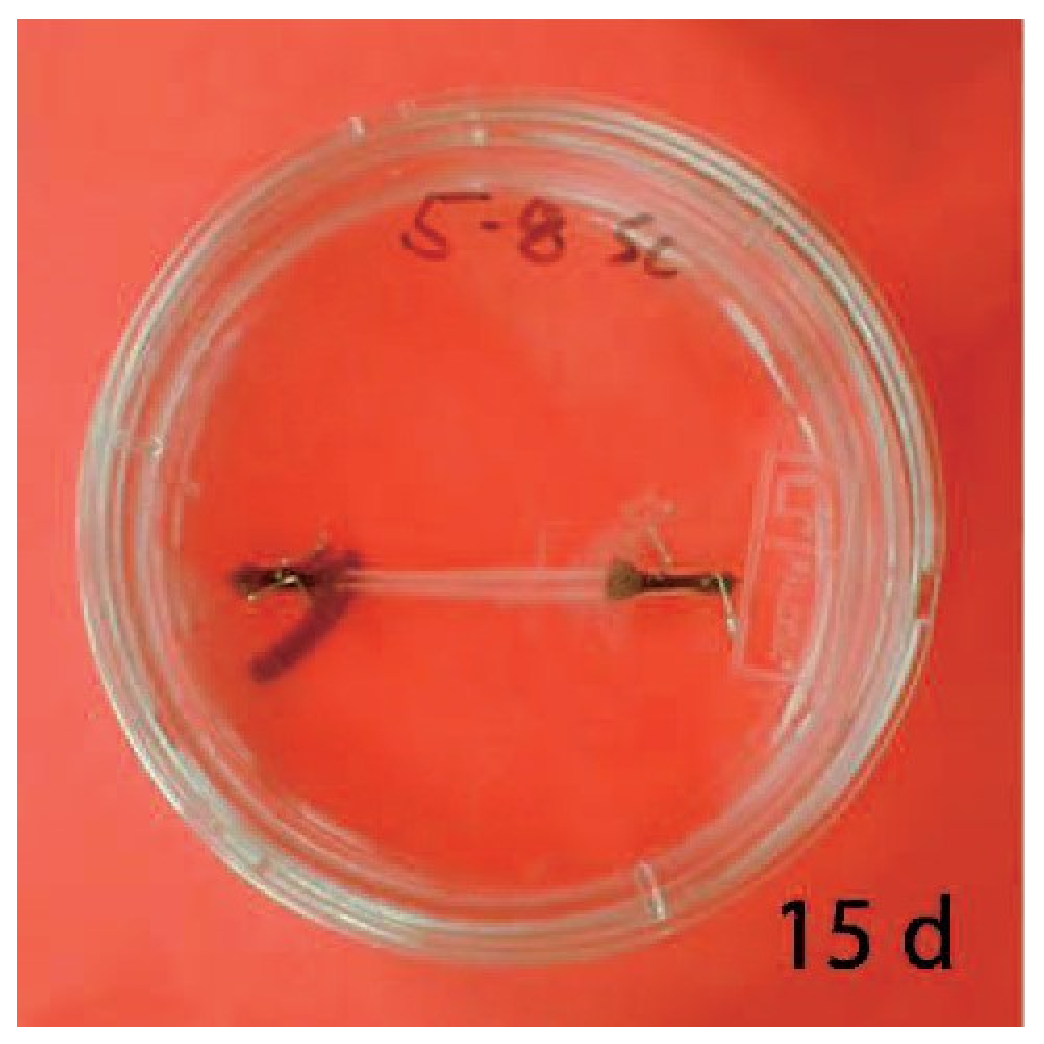
\includegraphics[width=0.6\textwidth]{images/experiments/one-construct}
\caption{Engineered tendon construct. See \citet{Calve:04} for
  details.} 
\label{engconst}
\end{figure}

\begin{figure}[!hpt]
  \centering
  \psfrag{D}{\small$1.1284$ mm}
  \psfrag{H}{\small$12.0$ mm}
  {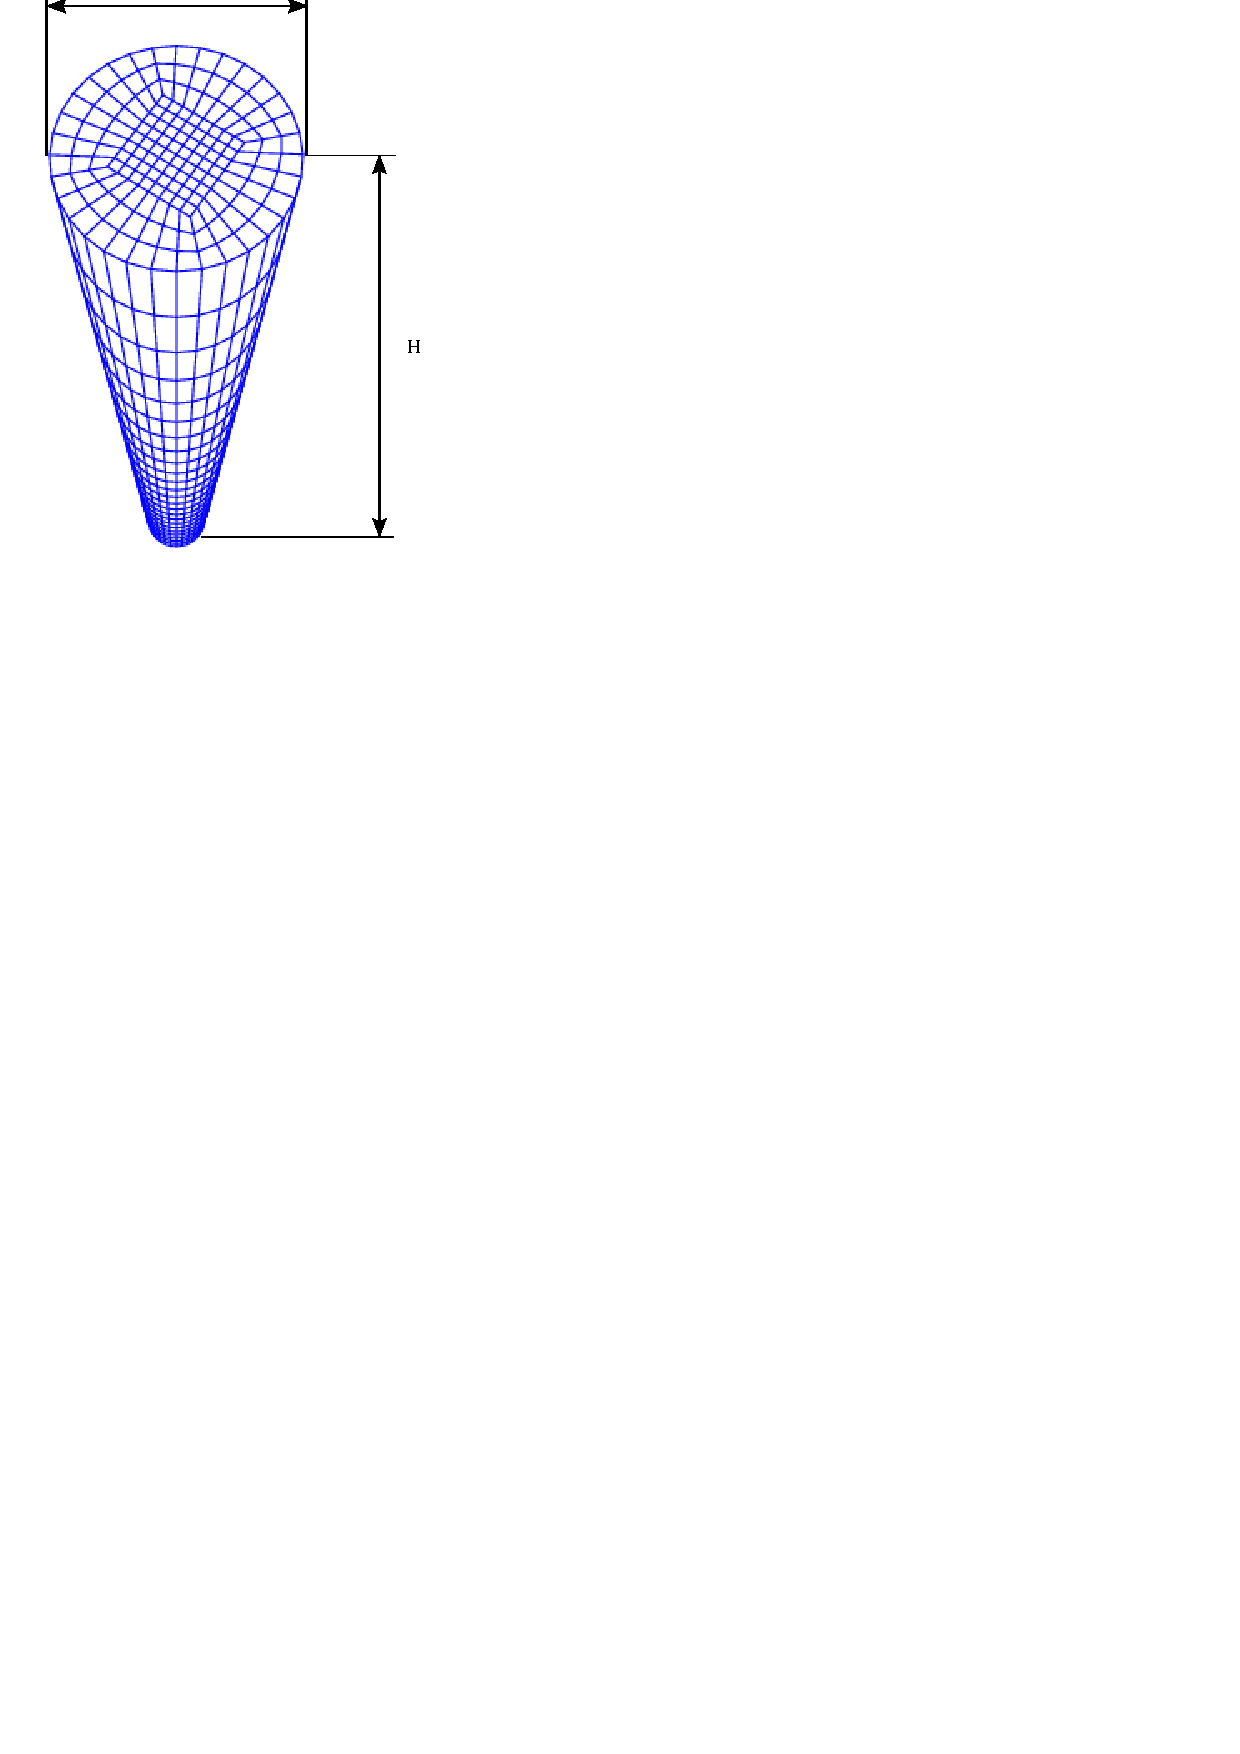
\includegraphics[width=0.4\textwidth]{images/examples/lagrangian/mesh}}
  \caption{The finite element mesh used in the computations.}
  \label{egmesh}
\end{figure}

The constitutive relation for the solid collagen follows
(\ref{wlcm-energy}). The constitutive relation for the fluid stress
follows (\ref{Pf}) with,

\begin{equation}
h(\rho^\mathrm{f}) =
\frac{1}{2}\kappa^\mathrm{f}\left(
\frac{\rho_{0_\mathrm{ini}}^\mathrm{f}}{\rho^\mathrm{f}}
- 1\right)^2,
\end{equation}

\noindent where $\kappa^\mathrm{f}$ is the fluid bulk modulus.

The
tissue is modelled as being fluid saturated in $\Omega_t$ at $t = 0$,
i.e. (\ref{saturation}$_1$) holds with
$\rho^\mathrm{f}_{0_\mathrm{sat}} =
\rho^\mathrm{f}_{0_\mathrm{ini}}$. However, the tissue is allowed to 
become unsaturated in $\Omega_t$ for $t > 0$ due to void formation. Then,
the conditions set out in (\ref{cavitation})
apply. The chemical potential is then given by
(\ref{fickeanmobility}). The numerical examples that follow discuss further
specialization of the constitutive relations to other cases discussed
in the preceding sections. The numerical values of parameters\footnote{The
  mobility tensor reported in Table~\ref{parameters} is an
  order-of-magnitude estimate 
  recalculated from \citet{Hanetal:2000} to correspond to the 
  mobility used in this paper. These authors reported a mean value of
  $0.927\times 10^{-14}$ s, with a range of $1.14\times
  10^{-14}--0.58\times 10^{-14}$ s in terms of the mobility used
  here. Theirs is the mobility parallel to the fiber direction in
  Rabbit Achilles tendon. Our usage of it is as an isotropic
  mobility. Using anisotropic mobilities, or different values from the
  reported range changes the result
  quantitatively, but not qualitatively.}  that
have been used appear in Table~\ref{parameters}.




The initial and boundary
conditions have been chosen in order to model a few common mechanical and
chemical interventions on engineered tissue. However, we will not
attempt detailed descriptions of experiments, choosing to focus
instead on results that can be directly related to the models. A more
detailed comparison with experiments is forthcoming in a separate
communication.



\section{Examples exploring the biphasic nature of porous soft tissue}
\label{biphasic-examples-1}

In these calculations, only two phases---fluid and collagen---are
included for the mass transport and mechanics. The parameters used in the analysis
are presented in Table~\ref{parameters}. 

%The mixing entropy of fluid in the mixture with collagen is
%written as $\eta_{\mathrm{mix}}^{f} = -\frac{k}{\sM^\mathrm{f}}
%\mathrm{log} (\frac{\rho^\mathrm{f}} {\rho})$, where
%$\sM^\mathrm{f}$ is the molecular weight of the fluid.

%\subsection{Using the appropriate configuration}
%\label{appropriate-configuration}



%% {\bf Unbounded pinching problem}

%% \subsection{Fluxes from different driving forces}
%% \label{flux-driving-forces}

%% The following contour plots represent the stress, and various
%% contributions to the total flux in the early stages of loading of
%% the model problem. Symmetry has been employed to model a single
%% quadrant of the cylinder.

%% The longitudinal stress, $\sigma_{33}$ in Figure \ref{stressfig}
%% arises from the stretch and the evolution in concentration.
%% \begin{figure}[!hpt]
%% \begin{minipage}[t]{7.5cm}
%% {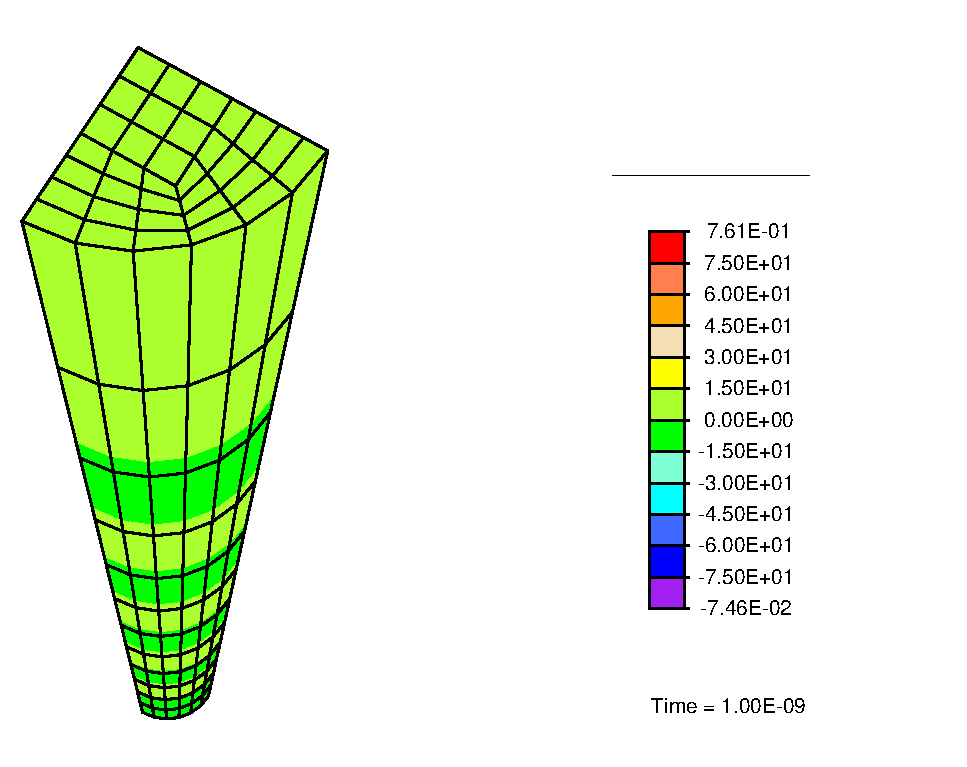
\includegraphics[width=7.5cm]{images/examples/lagrangian/preliminary/S33-1}} \hskip 3cm (a) 
%% \end{minipage}
%% \begin{minipage}[t]{7.5cm}
%% {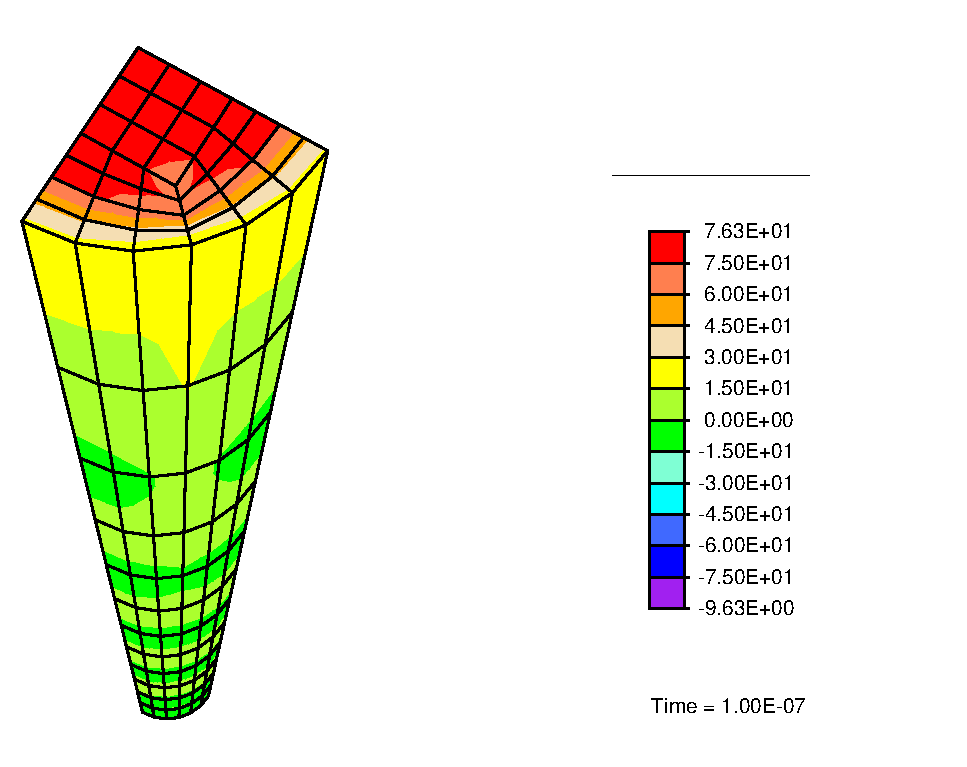
\includegraphics[width=7.5cm]{images/examples/lagrangian/preliminary/S33-100}} \hskip 3cm (b)
%% \end{minipage}
%% \caption{Longitudinal Cauchy stress, $\sigma_{33}$ (Pa) at $1
%% \,\mathrm{nanosec.}$ and $100\,\mathrm{nanosec.}$ after the
%% beginning of loading.} \label{stressfig}
%% \end{figure}

%% \begin{figure}[!hpt]
%% \begin{minipage}[t]{7.5cm}
%% {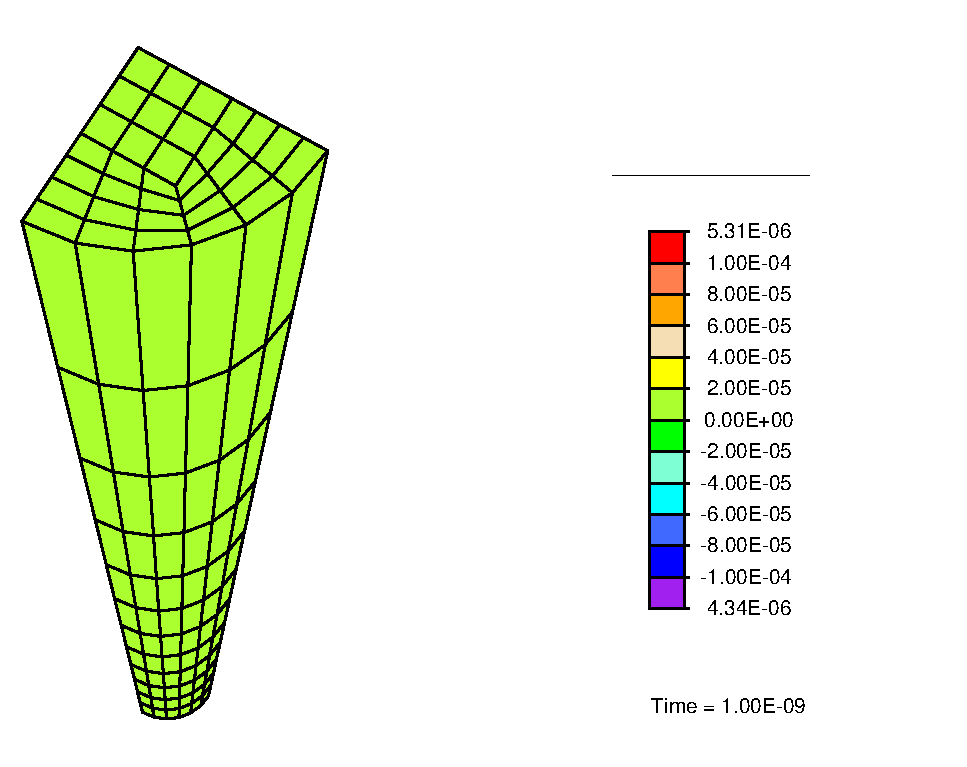
\includegraphics[width=7.5cm]{images/examples/lagrangian/preliminary/M1-1}} \hskip 3cm (a)
%% \end{minipage}
%% \begin{minipage}[t]{7.5cm}
%% {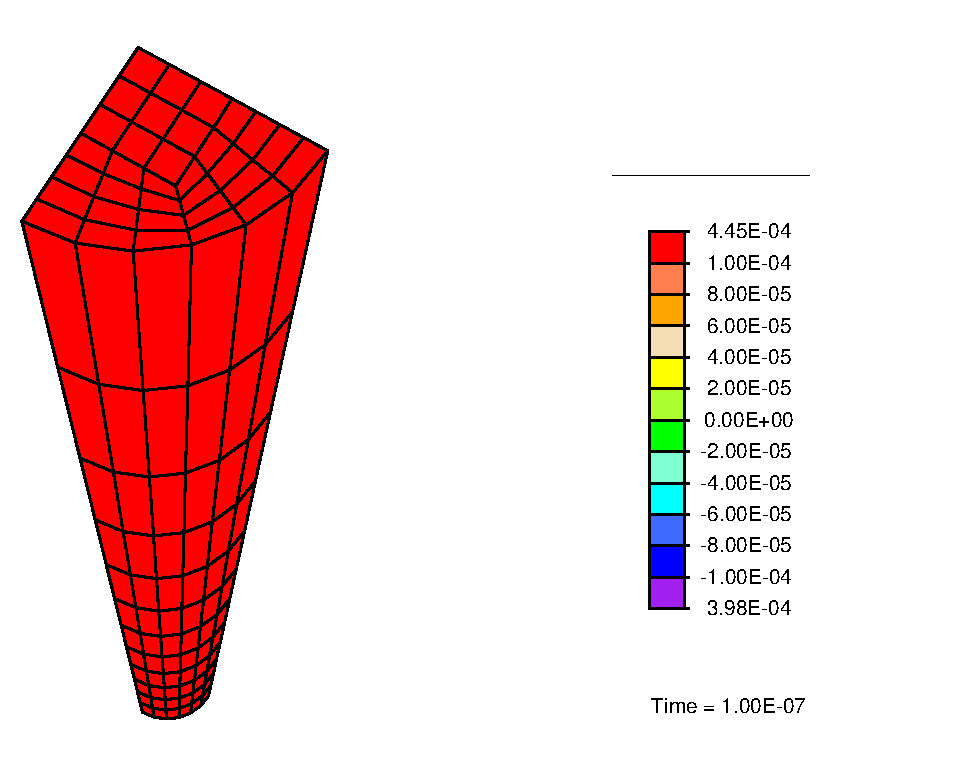
\includegraphics[width=7.5cm]{images/examples/lagrangian/preliminary/M1-100}} \hskip 3cm (b)
%% \end{minipage}
%% \caption[Stress gradient-driven flux]{Stress gradient-driven flux
%% ($\mathrm{kg.m}^{-2}\mathrm{sec}$) in the $\be_3$ direction at $1
%% \,\mathrm{nanosec.}$ and $100\,\mathrm{nanosec.}$ after the
%% beginning of loading. The positive values indicate an upward flux
%% corresponding to a tensile $\sigma_{33}$ wave travelling
%% downwards.} \label{M1fig}
%% \end{figure}

%% \begin{figure}[!hpt]
%% \begin{minipage}[t]{7.5cm}
%% {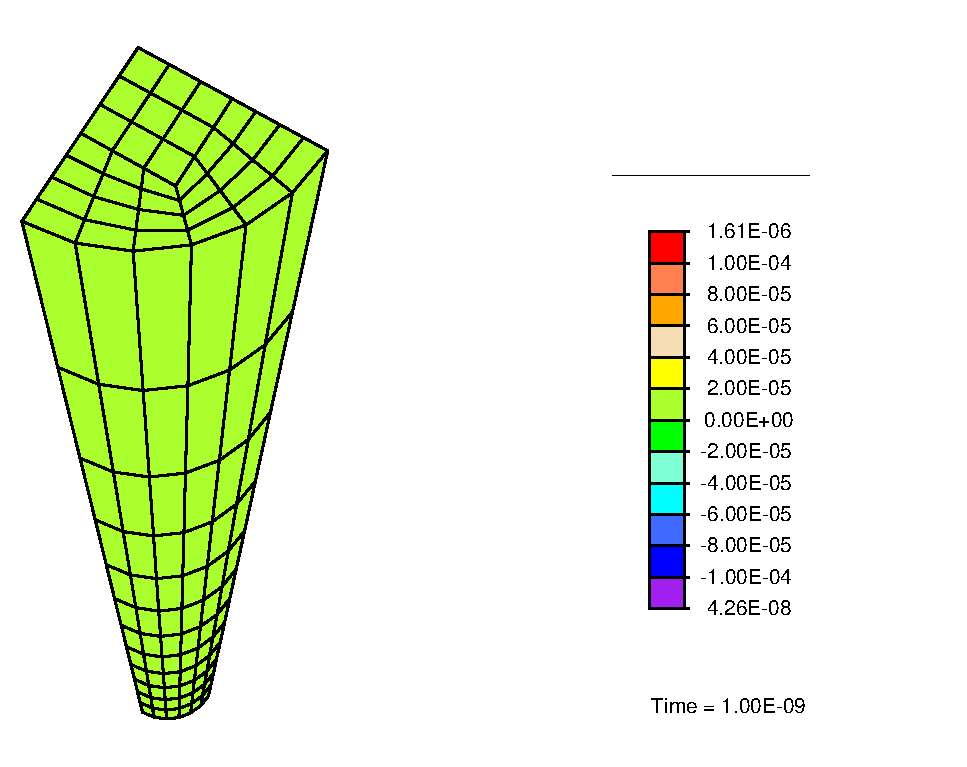
\includegraphics[width=7.5cm]{images/examples/lagrangian/preliminary/M2-1}} \hskip 3cm (a)
%% \end{minipage}
%% \begin{minipage}[t]{7.5cm}
%% {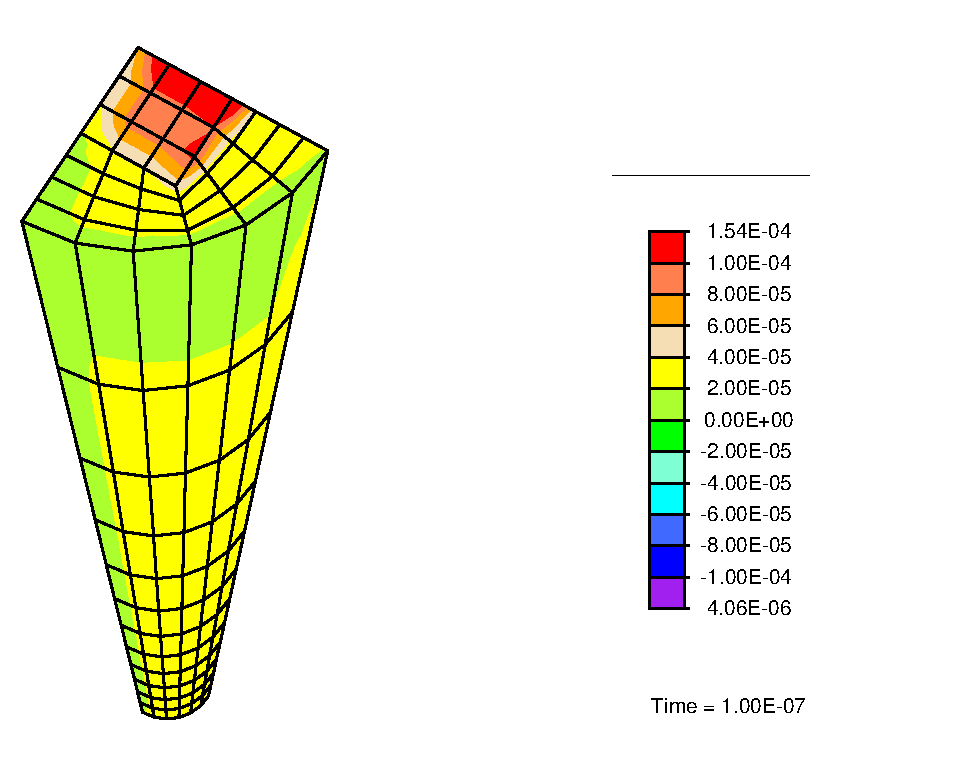
\includegraphics[width=7.5cm]{images/examples/lagrangian/preliminary/M2-100}} \hskip 3cm (b)
%% \end{minipage}
%% \caption{Internal energy gradient-driven flux,
%% ($\mathrm{kg.m}^{-2}\mathrm{sec}$) in the $\be_3$ direction at $1
%% \,\mathrm{nanosec.}$ and $100\,\mathrm{nanosec.}$ after the
%% beginning of loading. The positive values indicate an upward flux.
%% This corresponds to a lower energy near the top of the cylinder as
%% the tensile stress ($\sigma_{33}$) wave travels downward and
%% relaxes some of the strain energy of contraction.} \label{M2fig}
%% \end{figure}

%% \begin{figure}[!hpt]
%% \begin{minipage}[t]{7.5cm}
%% {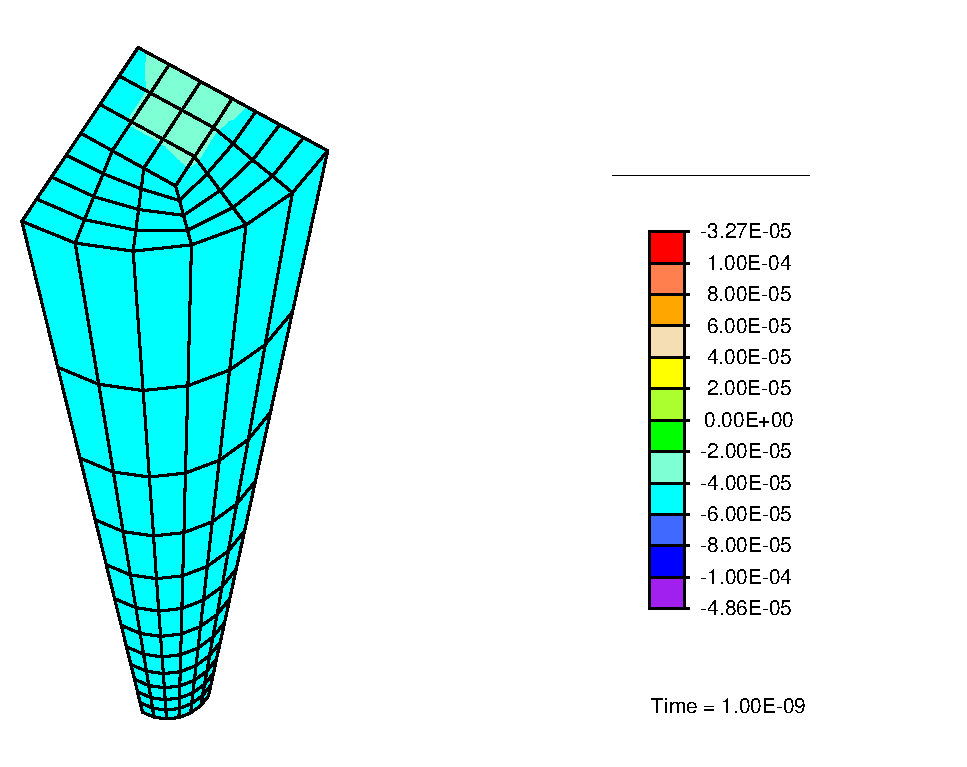
\includegraphics[width=7.5cm]{images/examples/lagrangian/preliminary/M3-1}} \hskip 3cm (a)
%% \end{minipage}
%% \begin{minipage}[t]{7.5cm}
%% {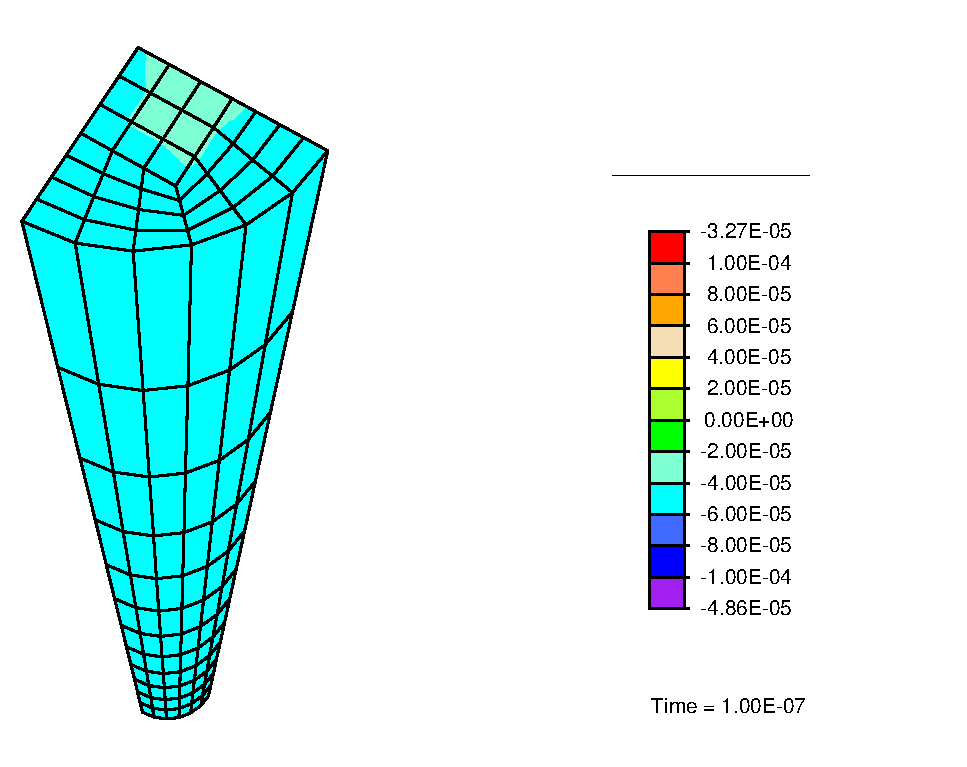
\includegraphics[width=7.5cm]{images/examples/lagrangian/preliminary/M3-100}} \hskip 3cm (b)
%% \end{minipage}
%% \caption{Gravity-driven flux ($\mathrm{kg.m}^{-2}\mathrm{sec}$) in
%% the $\be_3$ direction at $1 \,\mathrm{nanosec.}$ and
%% $100\,\mathrm{nanosec.}$ after the beginning of loading. The
%% negative values indicate a downward flux, due to the action of
%% gravity.} \label{M3fig}
%% \end{figure}

%% \begin{figure}[!hpt]
%% \begin{minipage}[t]{7.5cm}
%% {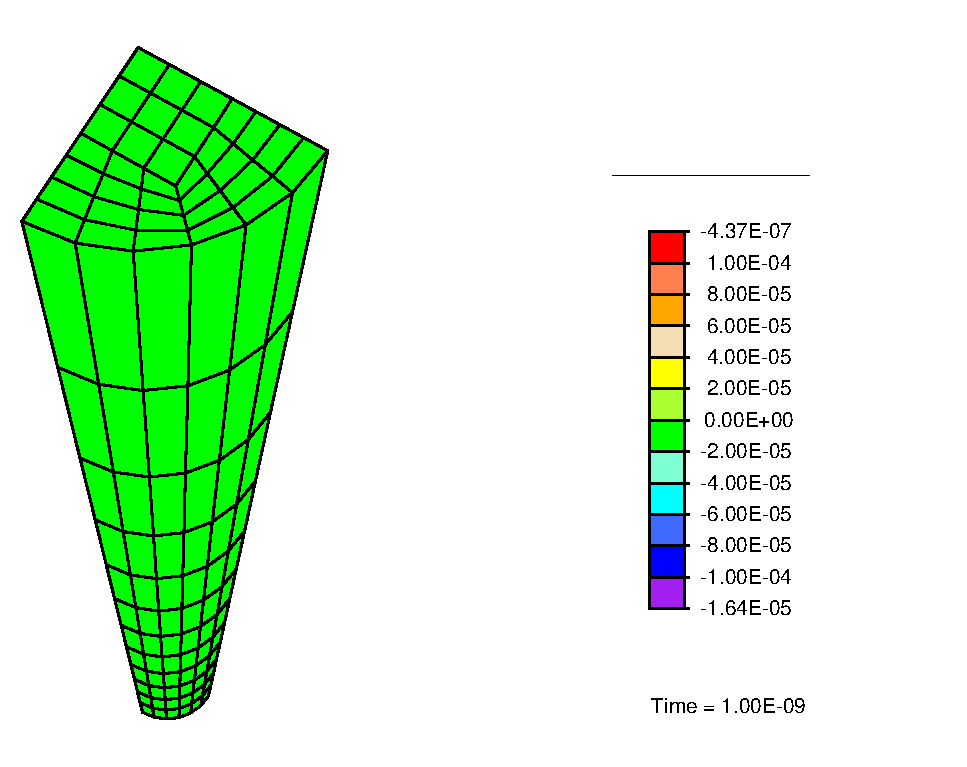
\includegraphics[width=7.5cm]{images/examples/lagrangian/preliminary/M4-1}} \hskip 3cm (a)
%% \end{minipage}
%% \begin{minipage}[t]{7.5cm}
%% {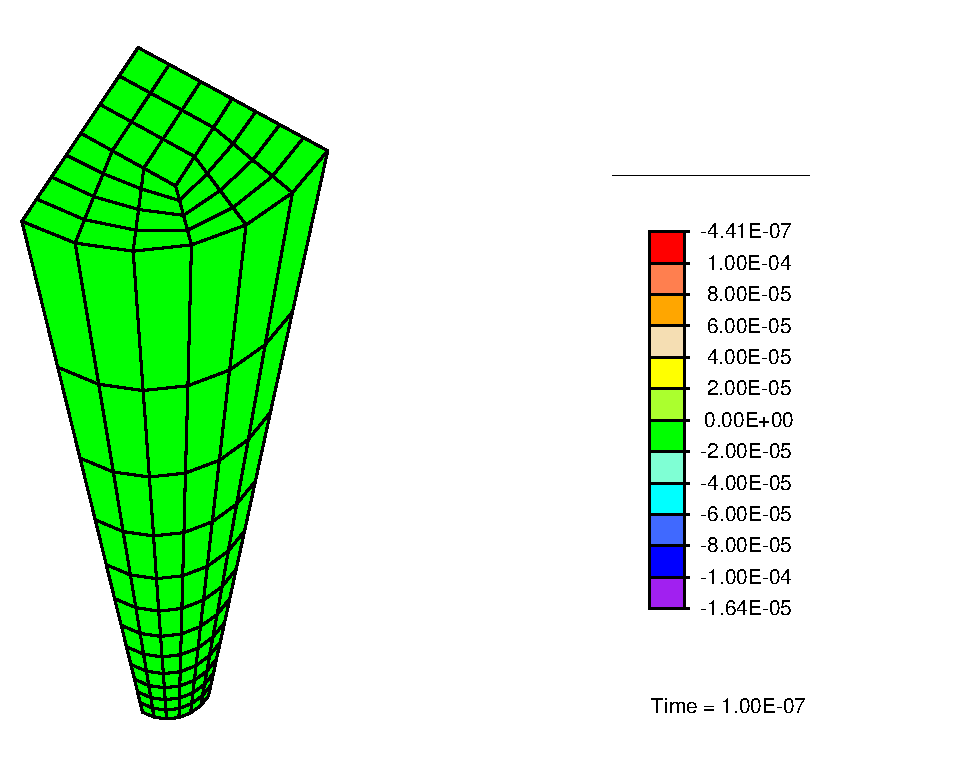
\includegraphics[width=7.5cm]{images/examples/lagrangian/preliminary/M4-100}} \hskip 3cm (b)
%% \end{minipage}
%% \caption{Inertia-driven flux ($\mathrm{kg.m}^{-2}\mathrm{sec}$) in
%% the $\be_3$ direction at $1 \,\mathrm{nanosec.}$ and
%% $100\,\mathrm{nanosec.}$ after the beginning of loading. The
%% negative values indicate a downward flux as the tissue accelerates
%% upward.} \label{M4fig}
%% \end{figure}

%% \begin{figure}[!hpt]
%% \begin{minipage}[t]{7.5cm}
%% {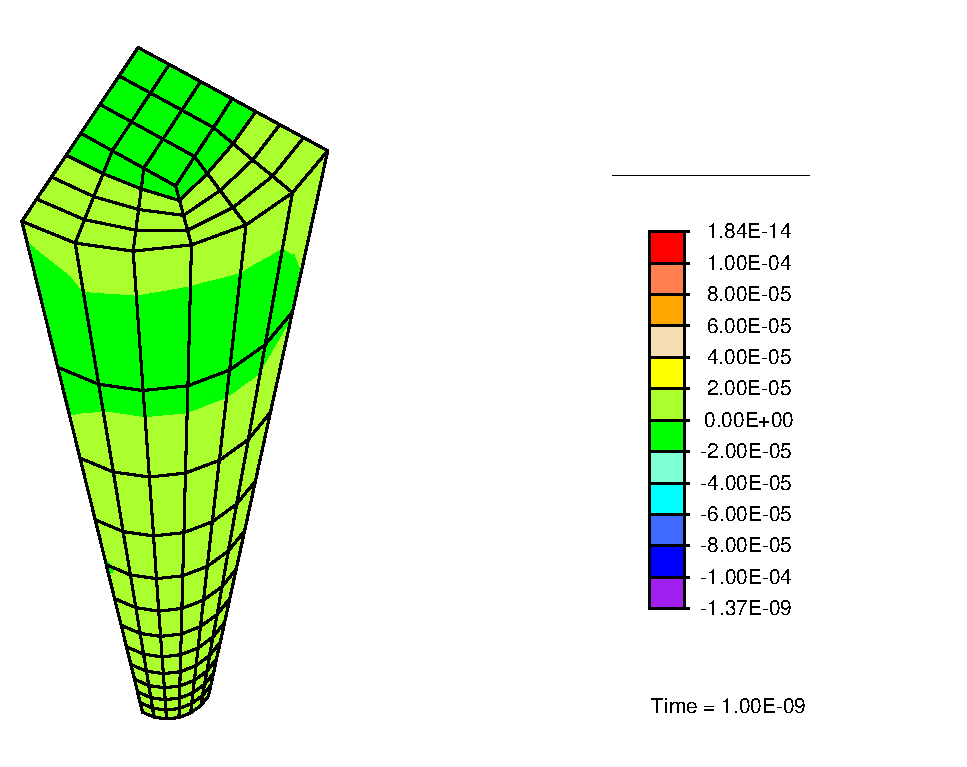
\includegraphics[width=7.5cm]{images/examples/lagrangian/preliminary/M5-1}} \hskip 3cm (a)
%% \end{minipage}
%% \begin{minipage}[t]{7.5cm}
%% {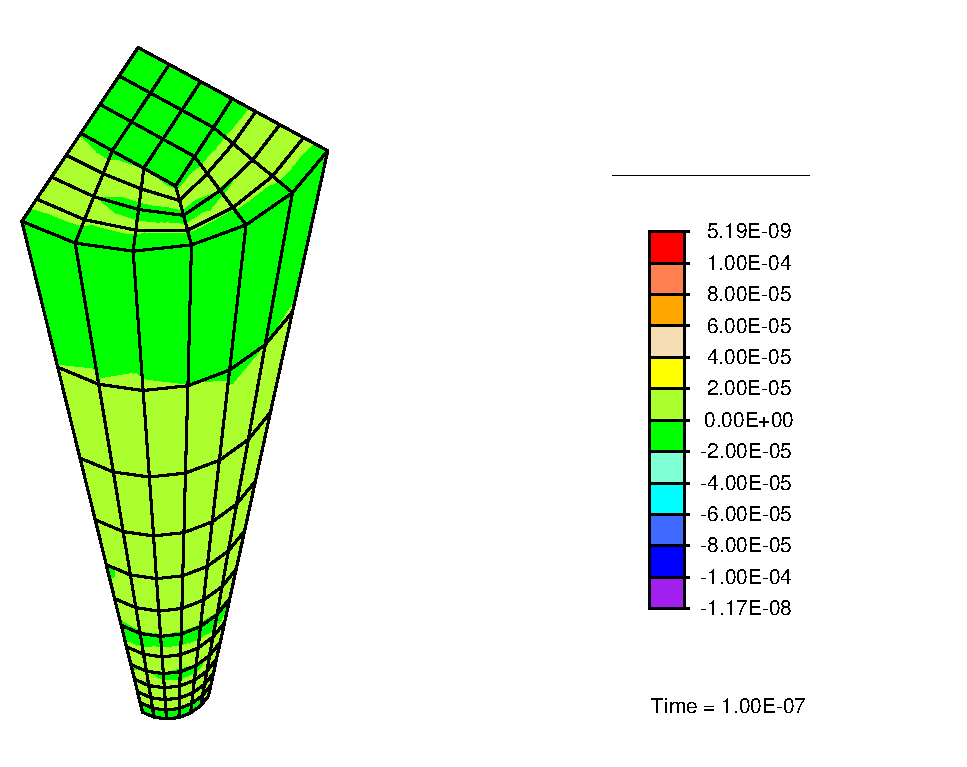
\includegraphics[width=7.5cm]{images/examples/lagrangian/preliminary/M5-100}} \hskip 3cm (b)
%% \end{minipage}
%% \caption{Concentration gradient-driven flux
%% ($\mathrm{kg.m}^{-2}\mathrm{sec}$) in the $\be_3$ direction at $1
%% \,\mathrm{nanosec.}$ and $100\,\mathrm{nanosec.}$ after the
%% beginning of loading. Note that the maximum and minimum values are
%% many orders of magnitude lower than for the other flux
%% contributions reported above. This is a demonstration of mechanics
%% influences dominating diffusion over the classical concentration
%% gradient contribution.} \label{M5fig}
%% \end{figure}

%% \begin{figure}[!hpt]
%% \begin{minipage}[t]{7.5cm}
%% {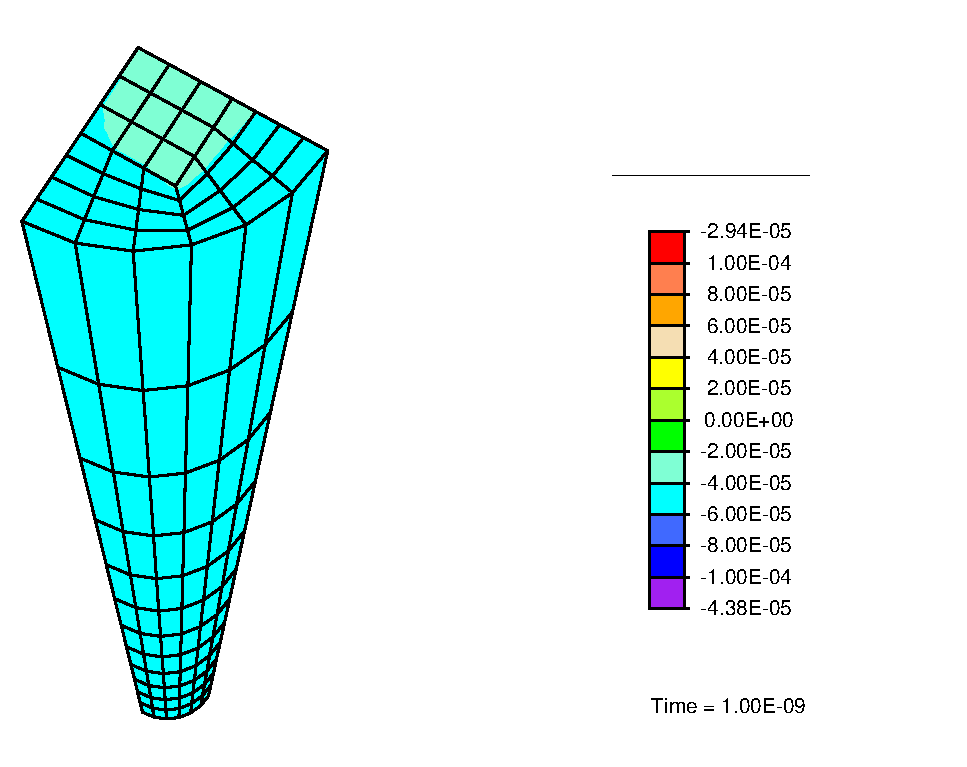
\includegraphics[width=7.5cm]{images/examples/lagrangian/preliminary/M-1}} \hskip 3cm (a)
%% \end{minipage}
%% \begin{minipage}[t]{7.5cm}
%% {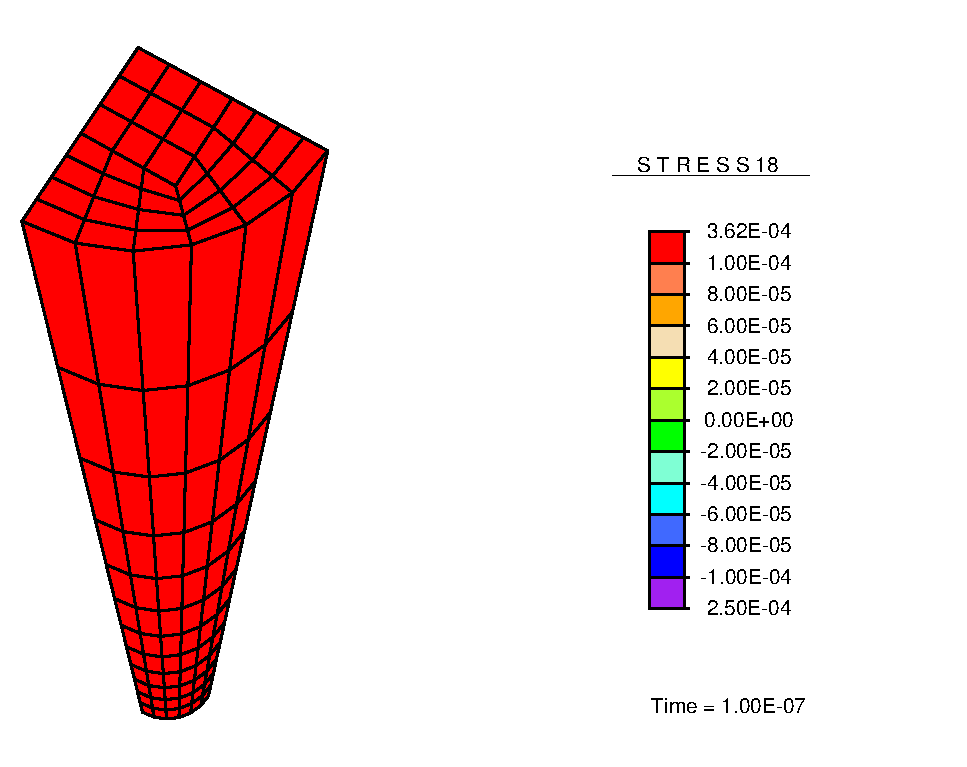
\includegraphics[width=7.5cm]{images/examples/lagrangian/preliminary/M-100}} \hskip 3cm (b)
%% \end{minipage}
%% \caption{Total flux ($\mathrm{kg.m}^{-2}\mathrm{sec}$) in the
%% $\be_3$ direction at $1 \,\mathrm{nanosec.}$ and
%% $100\,\mathrm{nanosec.}$ after the beginning of loading. The
%% positive values indicate an upward flux, dominated by the stress
%% gradient driven contribution.} \label{Mfig}
%% \end{figure}

%% The flux contributions in Figures \ref{M1fig}--\ref{Mfig} can be
%% summarized as follows: The fluid flux is dominated by the
%% contribution from the stress gradient in the $\be_3$ direction.
%% The latter arises as the stress ($\sigma_{33}$) wave of tension
%% travels down the cylinder in the first few microseconds after
%% application of the load (the time taken to travel the length of
%% the cylinder is $12 \,\mu\mathrm{sec}$). Additionally, as the
%% fluid concentration changes due to the flux, it causes a further
%% change in the stress (Section \ref{sect5}). Other flux terms are
%% qualitatively sensible; i.e., their directions are consistent with
%% the physics of the problem, as argued in each of the figure
%% captions\footnote{In order to compare the flux contributions, they
%% have all been plotted on the same scale: $-1\times
%% 10^{-4}--1\times 10^{-4} \,\mathrm{kg.m}^{-2}\mathrm{sec}$.
%% However the plots also show the maximum and minimum field values
%% at the top and bottom of the legend bars. These values represent a
%% better comparison of the relative flux magnitudes.}. There is some
%% loss of axial symmetry in a few of the plots due to the coarseness
%% of the finite element mesh for this example. It appears that
%% spatial oscillations in the solution lead to a further loss of
%% symmetry in Figures \ref{M2fig}b--\ref{M3fig}b and \ref{Mfig}a.
%% These oscillations arise due to large and dominant advective
%% terms, and need to be remedied by stabilized finite element
%% methods. Here, we only aim to demonstrate that various driving
%% forces for mass transport are in agreement with their theoretical
%% underpinnings in the paper. The resorption of the solid phase is
%% shown indirectly in Figure \ref{Pifig}. A positive fluid source,
%% $\Pi^\mathrm{f}$, means that $\Pi^\mathrm{s} < 0$. Since
%% $\Pi^\mathrm{s}$ is the only term balancing
%% $\partial\rho_0^\mathrm{s}/\partial t$ [see (\ref{massballocA})],
%% it follows that $\partial\rho_0^\mathrm{s}/\partial t < 0$.

%% \begin{figure}[!hpt]
%% \begin{minipage}[t]{7.5cm}
%% {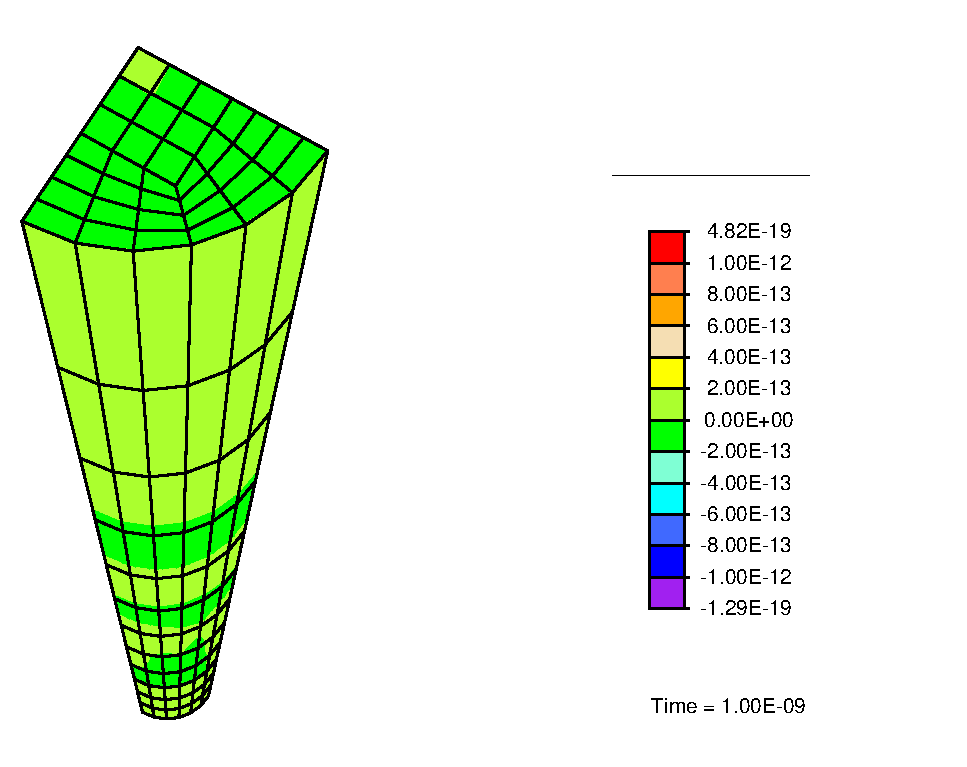
\includegraphics[width=7.5cm]{images/examples/lagrangian/preliminary/Pi-1}} \hskip 3cm (a)
%% \end{minipage}
%% \begin{minipage}[t]{7.5cm}
%% {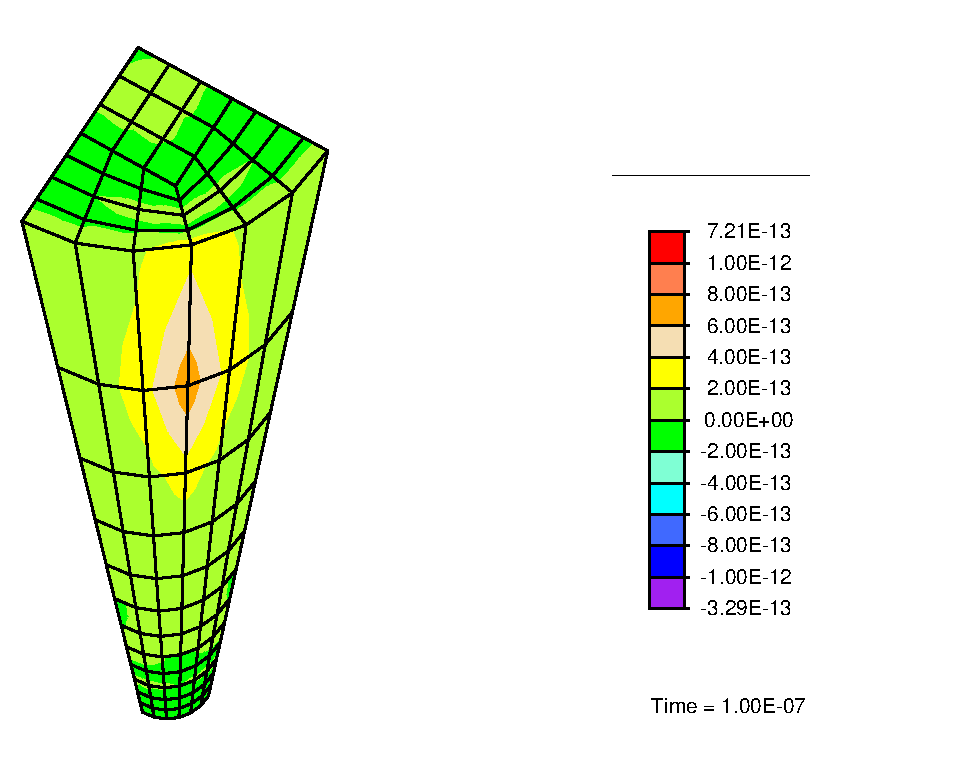
\includegraphics[width=7.5cm]{images/examples/lagrangian/preliminary/Pi-100}} \hskip 3cm (b)
%% \end{minipage}
%% \caption{Rate of fluid production, $\Pi^\mathrm{f}$
%% ($\mathrm{kg.m}^{-3}.\mathrm{sec}^{-1}$), at $1
%% \,\mathrm{nanosec.}$ and $100\,\mathrm{nanosec.}$ after the
%% beginning of loading. The positive values indicate that the local
%% fluid concentrations have fallen below their initial values.}
%% \label{Pifig}
%% \end{figure}

\subsection{The tendon under constriction}
\label{constriction-1}

In this example, the tendon immersed in a bath is subjected to the same
constrictive radial load as in Section~\ref{enzyme_kinetics_eg}. Since
that example demonstrated an insignificant amount of local collagen production
over this time scale, we have simplified the
problem by setting the source term $\Pi^\mathrm{c} = 0$. The total
duration of the simulation is 
10~s, and the radial strain is applied as a displacement boundary
condition, increasing linearly from no strain initially to the maximum
strain at time $t = 1~\mathrm{s}$. Again,
both the initial collagen 
concentration and the initial fluid concentration are 500~kg.m$^{-3}$
at every point in the tendon. This tendon is exposed to a bath where
the fluid concentration is 500~kg.m$^{-3}$.

\begin{figure}[ht]
  \centering
  \psfrag{A}{$\Omega_0$}
  \psfrag{B}{$\Omega_t$}
  \psfrag{C}{$\bF$}
  \psfrag{S}{\small Solid, `c'}
  \psfrag{F}{\small Fluid, `f'}
  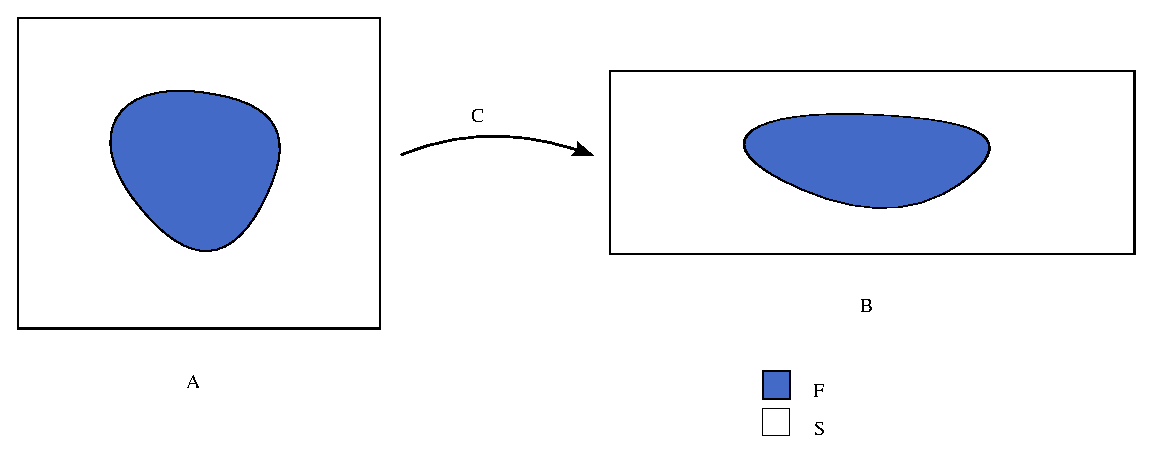
\includegraphics[width=0.8\textwidth]
                  {images/elucidation/homogeneous-deformation}
  \caption{Upper-bound model from strain homogenisation.}
  \label{upper-bound-model}
\end{figure}

\begin{figure}[ht]
  \centering
  \psfrag{A}{$\Omega_0$}
  \psfrag{B}{$\Omega_t$}
  \psfrag{C}{$\bF$}
  \psfrag{S}{\small Solid, `c'}
  \psfrag{F}{\small Fluid, `f'}
  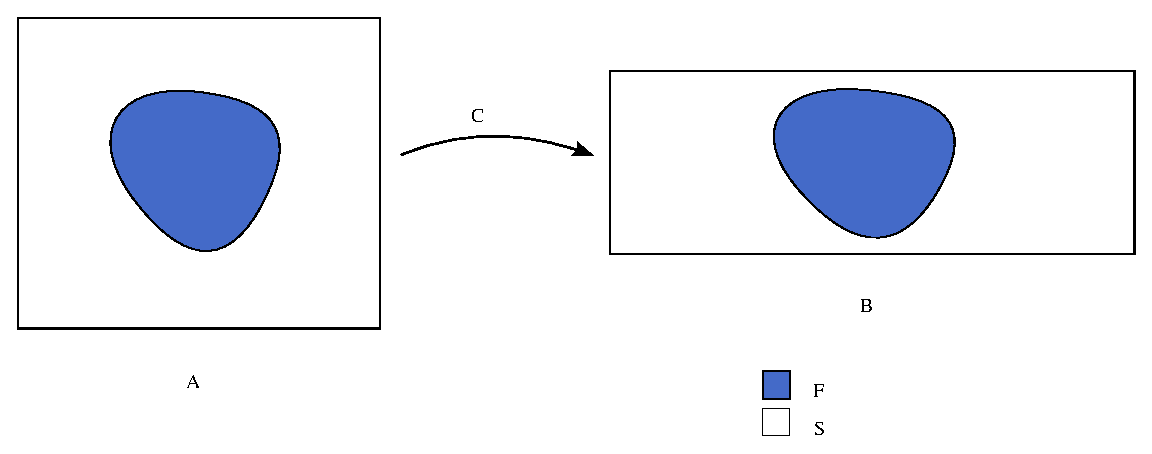
\includegraphics[width=0.8\textwidth]
                  {images/elucidation/homogeneous-stress}
  \caption{Lower-bound model from stress homogenisation.}
  \label{lower-bound-model}
\end{figure}

While solving the balance of momentum for the biphasic problem
of the solid collagen and a fluid phase, we currently treat the
tissue as a single entity and employ a summation of
Equation~(\ref{linearmombalance}) over both species. Additionally,
condition~(\ref{qrelation}) allows us to avoid constitutive
prescription of the momentum transfer terms between solid collagen and
fluid phases,
$\bq^\mathrm{c}$ and $\bq^\mathrm{f}$. This facilitates considerable
simplification of the 
problem, but such a treatment requires additional assumptions on the
detailed deformation of the constitutive phases of the tissue. An
explicit assumption we have drawn on thus far is the equality of
the deformation gradient of the solid collagen and pore spaces,
allowing us to use the deformation gradient
$\bF$, suitably decomposed to account for change in fluid
concentration, to model the fluid stress. This assumption and its 
consequences have been discussed in Sections \ref{bomass},
\ref{growthkinem}, \ref{satswel}, \ref{compfluid}, \ref{tensionfluid}
and \ref{incompfluid}. Since the imposition of a common deformation gradient
results in an upper bound for the 
effective stiffness of the tissue and magnitudes of the fluxes
established, we refer to it as the {\em upper bound model}. This
assumption plays a fundamental role in determining the fluid flux driven
by the fluid stress gradient.

\begin{figure}[!hpt]
  \centering
      {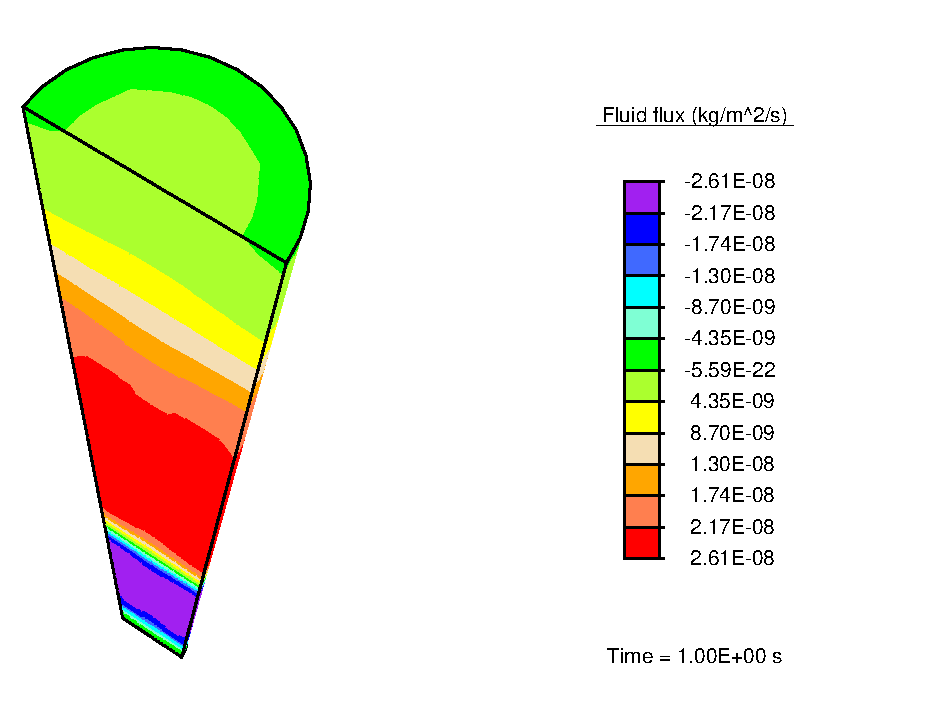
\includegraphics[width=0.8\textwidth]{images/examples/lagrangian/constriction/upper-bound-flux}}
      \caption{{\em Upper bound} fluid flux (kg.m$^{-2}$.s$^{-1}$) in
        the vertical direction at time $t=1$~s.}
      \label{eg2flux}
\end{figure}

\noindent For this upper bound model, Figure~\ref{eg2flux} shows the fluid flux in
the vertical direction at the final stage of the constriction phase of
the simulation, i.e. at time $t=1$~s. The flux values are positive
above the central plane, forcing fluid upward, and negative below,
forcing fluid fluid downward. This stress-gradient induced fluid flux
results in a reference concentration distribution of the fluid that is
higher near the top and bottom faces, as seen in Figure~\ref{eg2conc}.

\begin{figure}[!hpt]
  \centering
      {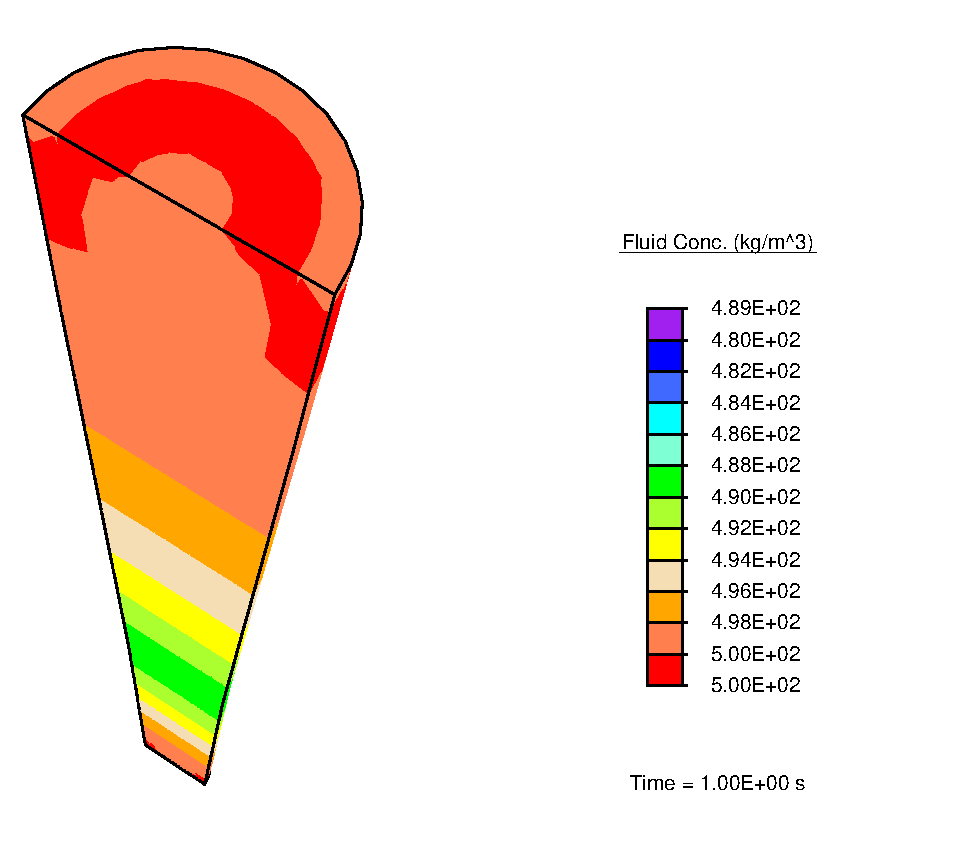
\includegraphics[width=0.8\textwidth]{images/examples/lagrangian/constriction/fluid-concentration}}
      \caption{Reference fluid concentration (kg.m$^{-3}$) at time
      $t=1$~s.}
      \label{eg2conc}
\end{figure}

As a result, these regions would have seen a higher production of
collagen, or preferential growth, in the presence of non-zero source
terms. As discussed in Section~\ref{curr-ref-mb}, the mass transport
equations are solved in the current configuration, where physical
boundary conditions can be set directly. The values reported in
Figure~\ref{eg2conc} are pulled back from the current
configuration. The current concentrations do not change for this
boundary value problem. 

Solving a problem of this nature in the
reference configuration using $\rho_0^\mathrm{f} = $ const. as the
boundary condition to represent immersion of the tendon in a fluid bath
yields non-physical results, such as an unbounded flow. This occurs
since the imposed strain gradient causes a stress gradient in the
fluid that does not decay. The imposed boundary condition on $\rho_0^\mathrm{f}$
prevents a redistribution of concentration that would have provided an
opposing, internal gradient of stress, which in turn would drive the
flux to vanish.

The tendon is held fixed in the radial direction after the
constriction phase. The applied stress sets up a pressure wave in the
fluid travelling toward the top and bottom faces. As the fluid leaves
these surfaces, we observe that the tendon relaxes. This is seen in
Figure~\ref{topdisp}, which plots the vertical displacement of the top
face with time, showing a decrease in height of the tendon after the
constriction phase. We keep the centre of the bottom face of the
tendon fixed.

\begin{figure}[!hpt]
  \centering
      {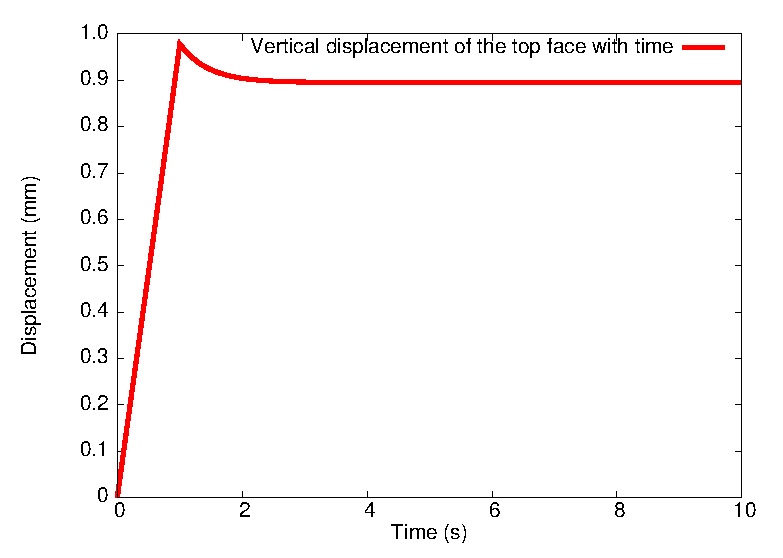
\includegraphics[width=0.8\textwidth]{images/examples/lagrangian/constriction/top-vertical-displacement}}
      \caption{Relaxation of the top face of the tendon after the
      constriction phase.}
      \label{topdisp}
\end{figure}

In order to define a range of the magnitude of fluid flux, we now
introduce the {\em lower bound model} (on effective stiffness of the
tissue and, consequently, the magnitude of the fluid flux). For this lower bound, we
replace the earlier strain homogenisation requirement with a stress
homogenisation requirement, {\em viz.} equating the hydrostatic stress
of the solid phase and the fluid pressure in the current
configuration:

\begin{equation}
p^{\mathrm{f}}=\frac{1}{3} \mathrm{\small{tr}}[\Bsigma^{c}],
\label{equalpr}
\end{equation}

\noindent where $p^{\mathrm{f}}$ is the fluid pressure in the current
configuration, $\mbox{\small{tr}[\textbullet]}$ is the trace operator, and
$\Bsigma^{c}=\frac{1}{\mathrm{J^{c}}} \bP^{\mathrm{c}}
\bF^{\mathrm{c}^{\mathrm{T}}}$ is the Cauchy stress of the solid. The
Cauchy stress of an ideal fluid can be defined from its current
pressure as \mbox{$\Bsigma^{f}= p^{\mathrm{f}} \bone$.}
Figure~{\ref{lowerbound}} reports the value of the vertical flux under
the lower bound modelling assumption, using boundary conditions identical to the
previous calculation at time $t=1$~s, the final stage of the
constriction phase of the simulation. 


\begin{figure}[!hpt]
  \centering
      {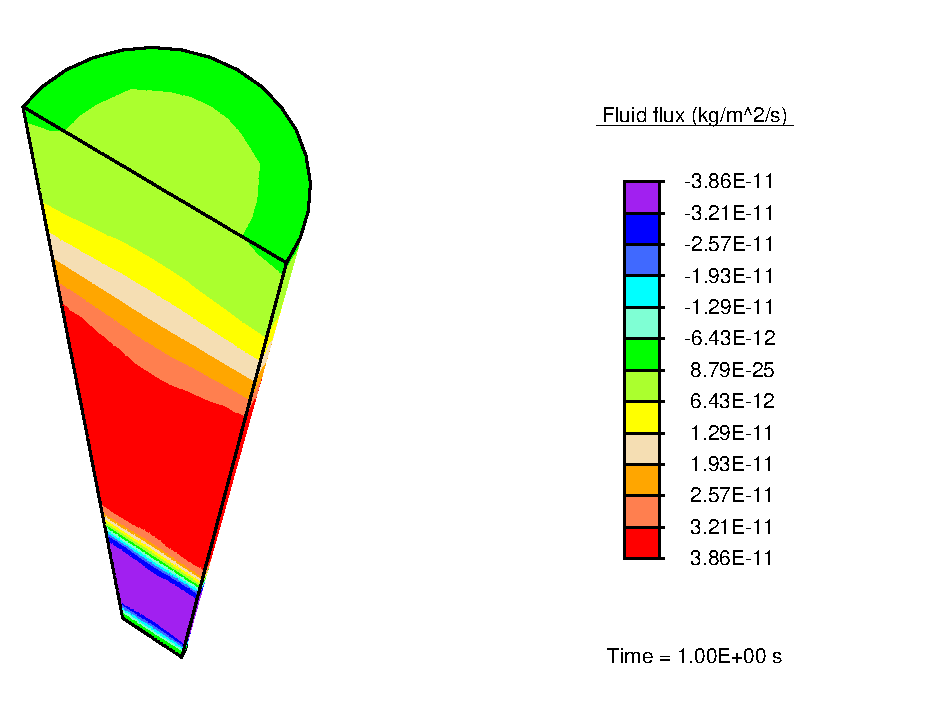
\includegraphics[width=0.8\textwidth]{images/examples/lagrangian/constriction/lower-bound-flux}}
      \caption{{\em Lower bound} fluid flux (kg.m$^{-2}$.s$^{-1}$) in
        the vertical direction at time $t=1$~s.}
      \label{lowerbound}
\end{figure}

The fluid flux values reported in Figures~\ref{eg2flux} and
\ref{lowerbound} (corresponding to the upper and lower bound modelling
assumptions, respectively) are qualitatively similar, but differ by
about three orders of magnitude. This wide range points to the
importance of imposing the appropriate mechanical coupling model
between interacting phases. Note, however, that we have computed
bounds for the 
range of possible fluid flux values under the specified mechanical
loading. Recall, furthermore, that the example in Section
\ref{enzyme_kinetics_eg} used the upper bound model, and yet resulted
in no discernible advective solute transport. This suggests strongly
that, given the parameters in Table \ref{parameters}, convective
transport of nutrients in tendons is dominated by diffusive
transport. In future work, we will detail models that result in precise
field values for the fluxes, which will replace the upper and lower
bounds discussed here.  


This numerical example also points to the fact that a convenient
measure of the strength of 
coupling between the mechanics and mass transport equations is the
ratio of the variation in hydrostatic stress of the fluid to that of
the solid. In the lower bound case, where the fluid response is
defined by Equation~(\ref{equalpr}), it is instructive to note that
this ratio is unity. As a result, it is seen that the lower bound case
exhibits significantly weaker coupling than the upper bound case. In
the latter, variation in the common deformation gradient, $\delta
\bF$, causes instantaneous variation in \mbox{$\delta p^{\mathrm{f}} \approx
  O(\kappa^{\mathrm{f}} \delta \bF:\bF^{-\mathrm{T}})$} and in
\mbox{$\frac{1}{3} \delta\mathrm{\small{tr}}[\Bsigma^{c}] \approx
  O(\kappa^{\mathrm{c}} \delta \bF:\bF^{-\mathrm{T}})$}, where
$\kappa^{\mathrm{c}}$ is the bulk modulus of the solid. The ratio
$\frac{\delta p^{\mathrm{f}}}{\frac{1}{3} \delta
  \mathrm{\small{tr}}[\Bsigma^{c}]}$ is therefore \mbox{$\approx
O(\kappa^{\mathrm{f}}/\kappa^{\mathrm{c}}) \gg 1$}.

The strength of coupling between the equations plays a principal role
in the rate of convergence of the solution, as observed in
Table~\ref{resnorms}, where the residual norms of the equilibrium
equation (and
corresponding CPU times in seconds for an Intel\textregistered Xeon
3.4 GHz machine) are reported for the first 8 iterations of each of
the two cases. Recall that the staggered scheme involves solution of
the mechanics equation 
keeping the concentrations fixed, and the mass transport equation
keeping the displacements fixed, in turn, until the solution
converges. The table does not report the value of the residual norms
arising from the solution of the mass transport equation for the
fluid, which occurs after each reported solve of the of the mechanics
equation. Although the initial mechanics residual norms in successive
passes are decreasing linearly in both cases, the rapid decrease in
this quantity in
the weakly-coupled case ensures convergence in far fewer iterations
than the strongly coupled case. Thus, the corresponding CPU times
reported are also lower for the weakly coupled case. This is
advantageous. In addition to being more physical, as argued at
the beginning of Section \ref{swelling} immediately below, the lower
bound, weakly-coupled case makes it feasible to drive 
problems to longer, physiologically-relevant time-scales through the use
of larger time steps.

\begin{table}
\centering
\begin{tabular}{|r|c|c|c|c|}
  \hline
  Pass & \multicolumn{2}{c|}{Strongly coupled} &
         \multicolumn{2}{c|}{Weakly coupled}\\
  \cline{2-5} & Residual & CPU (s) & Residual & CPU (s)\\
  \hline\hline 
1     & $ 2.138\times 10^{-02}$ &   29.16   & $6.761 \times 10^{-04}$  &    28.5 \\
      & $ 3.093\times 10^{-04}$ &   55.85   & $1.075 \times 10^{-04}$  &    55.1 \\
      & $ 2.443\times 10^{-06}$ &   82.37   & $4.984 \times 10^{-06}$  &    81.8 \\
      & $ 2.456\times 10^{-08}$ &  109.61   & $1.698 \times 10^{-08}$  &   107.9 \\
      & $ 4.697\times 10^{-14}$ &  135.83   & $3.401 \times 10^{-13}$  &   134.1 \\
      & $ 1.750\times 10^{-16}$ &  163.18   & $1.1523\times 10^{-17}$  &   161.1 \\
\hline                                    
2     & $ 5.308\times 10^{-06}$ &  166.79   & $5.971 \times 10^{-08}$  &  192.5  \\
      & $ 4.038\times 10^{-10}$ &  193.36   & $4.285 \times 10^{-11}$  &  218.6  \\
      & $ 1.440\times 10^{-14}$ &  220.45   & $2.673 \times 10^{-15}$  &  246.1  \\
      & $ 4.221\times 10^{-17}$ &  247.04   & $                    $   &  \\
\hline                                    
3     & $ 5.186\times 10^{-06}$ &  250.62   & $2.194 \times 10^{-09}$  &  277.3  \\
      & $ 3.852\times 10^{-10}$ &  277.44   & $2.196 \times 10^{-13}$  &  304.2   \\
      & $ 1.369\times 10^{-14}$ &  304.16   & $1.096 \times 10^{-17}$  &  331.6   \\
      & $ 4.120\times 10^{-17}$ &  331.47   & $                    $   &  \\
\hline                                    
4     & $ 5.065\times 10^{-06}$ &  335.16   & $8.160 \times 10^{-11}$  &  363.2 \\ 
      & $ 3.674\times 10^{-10}$ &  362.24   & $7.923 \times 10^{-15}$  &  390.2 \\
      & $ 1.300\times 10^{-14}$ &  388.79   & $                    $   &  \\
      & $ 4.021\times 10^{-17}$ &  416.08   & $                    $   &  \\
\hline                                    
5     & $ 4.948\times 10^{-06}$ &  419.59   & $3.078 \times 10^{-12}$  &  421.4 \\
      & $ 3.503\times 10^{-10}$ &  446.24   & $3.042 \times 10^{-16}$  &  448.6 \\
      & $ 1.236\times 10^{-14}$ &  473.20   & $                    $   &  \\
      & $ 3.924\times 10^{-17}$ &  500.85   & $                    $   &  \\
\hline                                    
6     & $ 4.832\times 10^{-06}$ &  504.65   & $1.179 \times 10^{-13}$  &  479.9 \\
      & $ 3.340\times 10^{-10}$ &  531.28   & $1.291 \times 10^{-17}$  &  507.0 \\
      & $ 1.174\times 10^{-14}$ &  558.17   & $                    $   &  \\
      & $ 3.829\times 10^{-17}$ &  585.27   & $                    $   &  \\
\hline                                    
7     & $ 4.720\times 10^{-06}$ &  589.01   & $4.592 \times 10^{-15}$  &  537.8 \\
      & $ 3.184\times 10^{-10}$ &  616.24   & $5.152 \times 10^{-18}$  &  564.6 \\
      & $ 1.116\times 10^{-14}$ &  643.29   & $                    $   &  \\
      & $ 3.737\times 10^{-17}$ &  670.83   & $                    $   &  \\
\hline                                    
8     & $ 4.609\times 10^{-06}$ &  674.46   & $1.816 \times 10^{-16}$  &  595.5  \\
      & $ 3.034\times 10^{-10}$ &  701.74   & $5.040 \times 10^{-18}$  &  622.3  \\
      & $ 1.060\times 10^{-14}$ &  727.74   & $                    $   &  \\
      & $ 3.646\times 10^{-17}$ &  755.58   & $                    $   &  \\
\hline
\end{tabular}
\caption{Mechanics equation residual norms and corresponding CPU times
  in seconds for the first 8 passes of each of the two cases for a
  typical time increment, $\Delta t=$ 0.1 s.}
\label{resnorms}
\end{table}

%% \subsubsection{Upper bound model}
%% \label{upper-bound}

%% \subsubsection{Lower bound model}
%% \label{lower-bound}

\subsection{A swelling problem}
\label{swelling-1}

\begin{figure}[!hpt]
  \centering
     {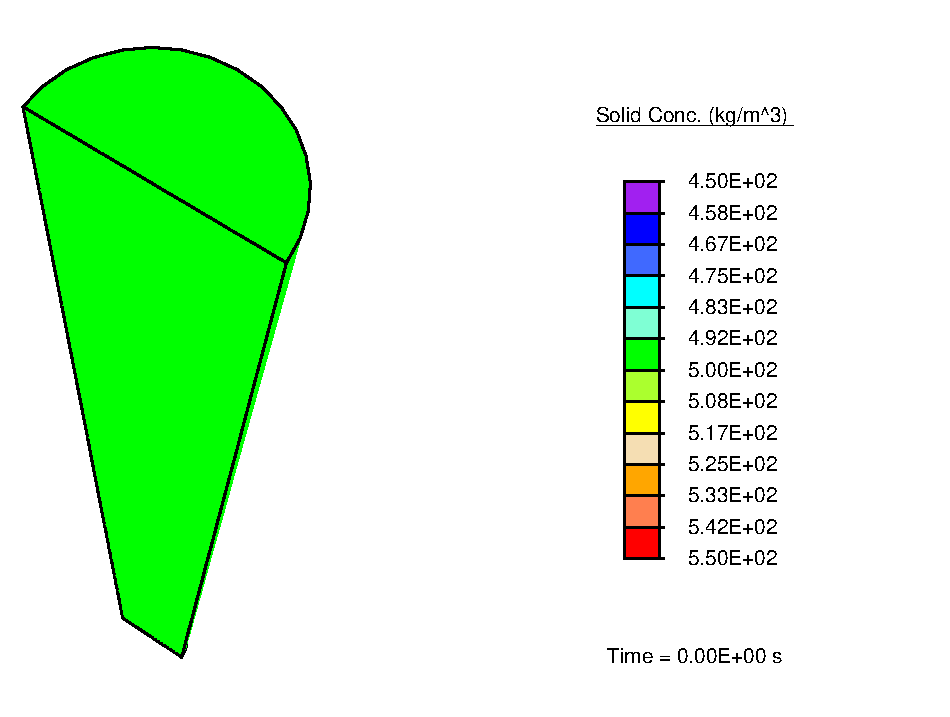
\includegraphics[width=0.8\textwidth]{images/examples/lagrangian/swelling/before-growth}}
     \caption{The collagen initial concentration (kg.m$^{-3}$).}
     \label{before_growth}
\end{figure}

\begin{figure}[!hpt]
  \centering
     {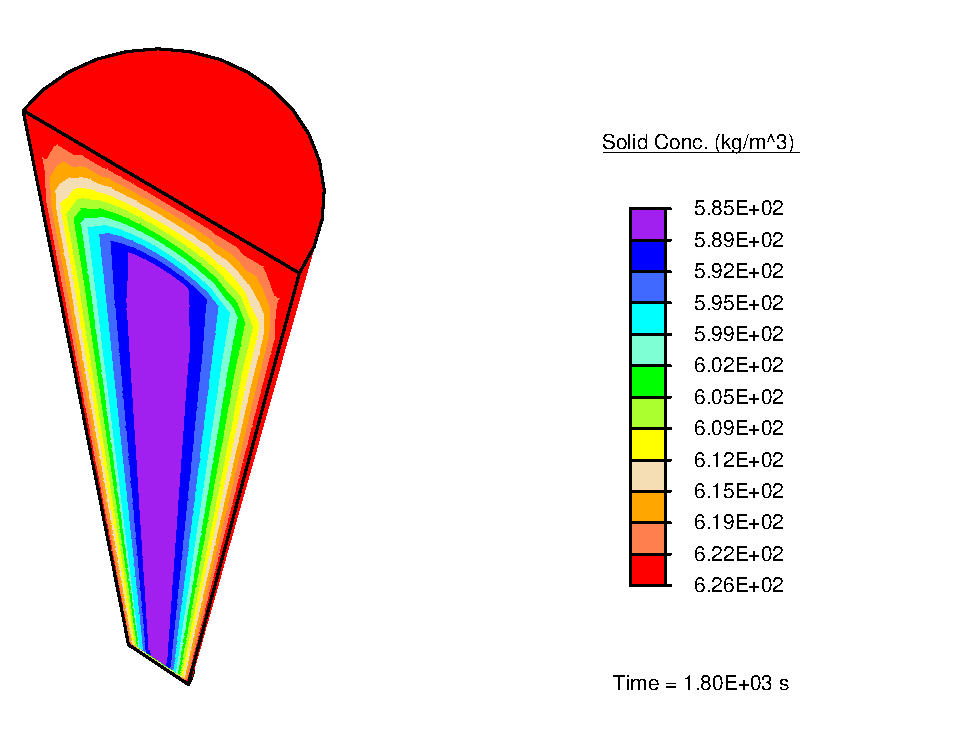
\includegraphics[width=0.8\textwidth]{images/examples/lagrangian/swelling/after-growth}}
     \caption{The collagen concentration (kg.m$^{-3}$) after 1800~s.}
     \label{after_growth}
\end{figure}

\begin{figure}[!hpt]
  \centering
     {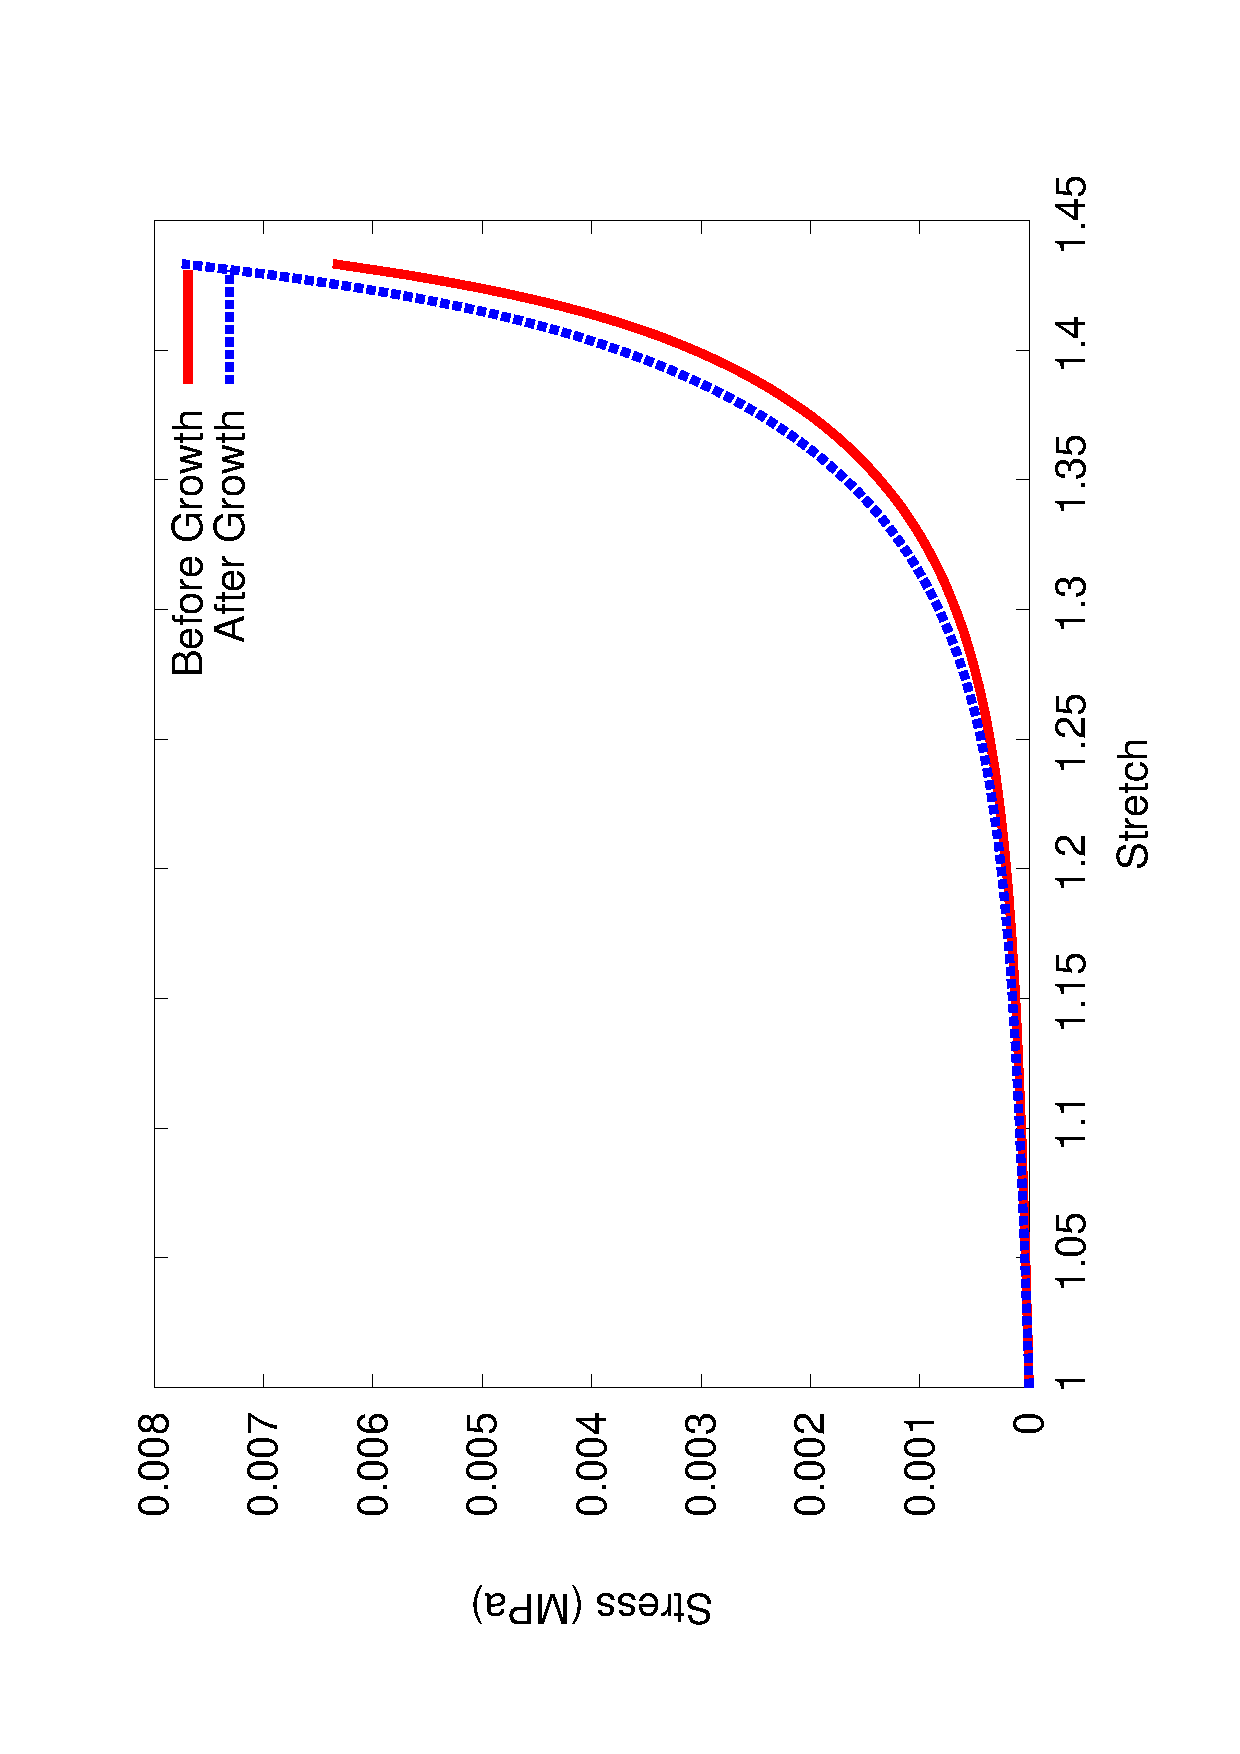
\includegraphics[angle=270,width=0.8\textwidth]{images/examples/lagrangian/swelling/stress-stretch}}
     \caption{The stress (Pa) vs stretch curves before and after
       growth.}
     \label{stress_strain}
\end{figure}

\begin{figure}[!hpt]
  \centering
     {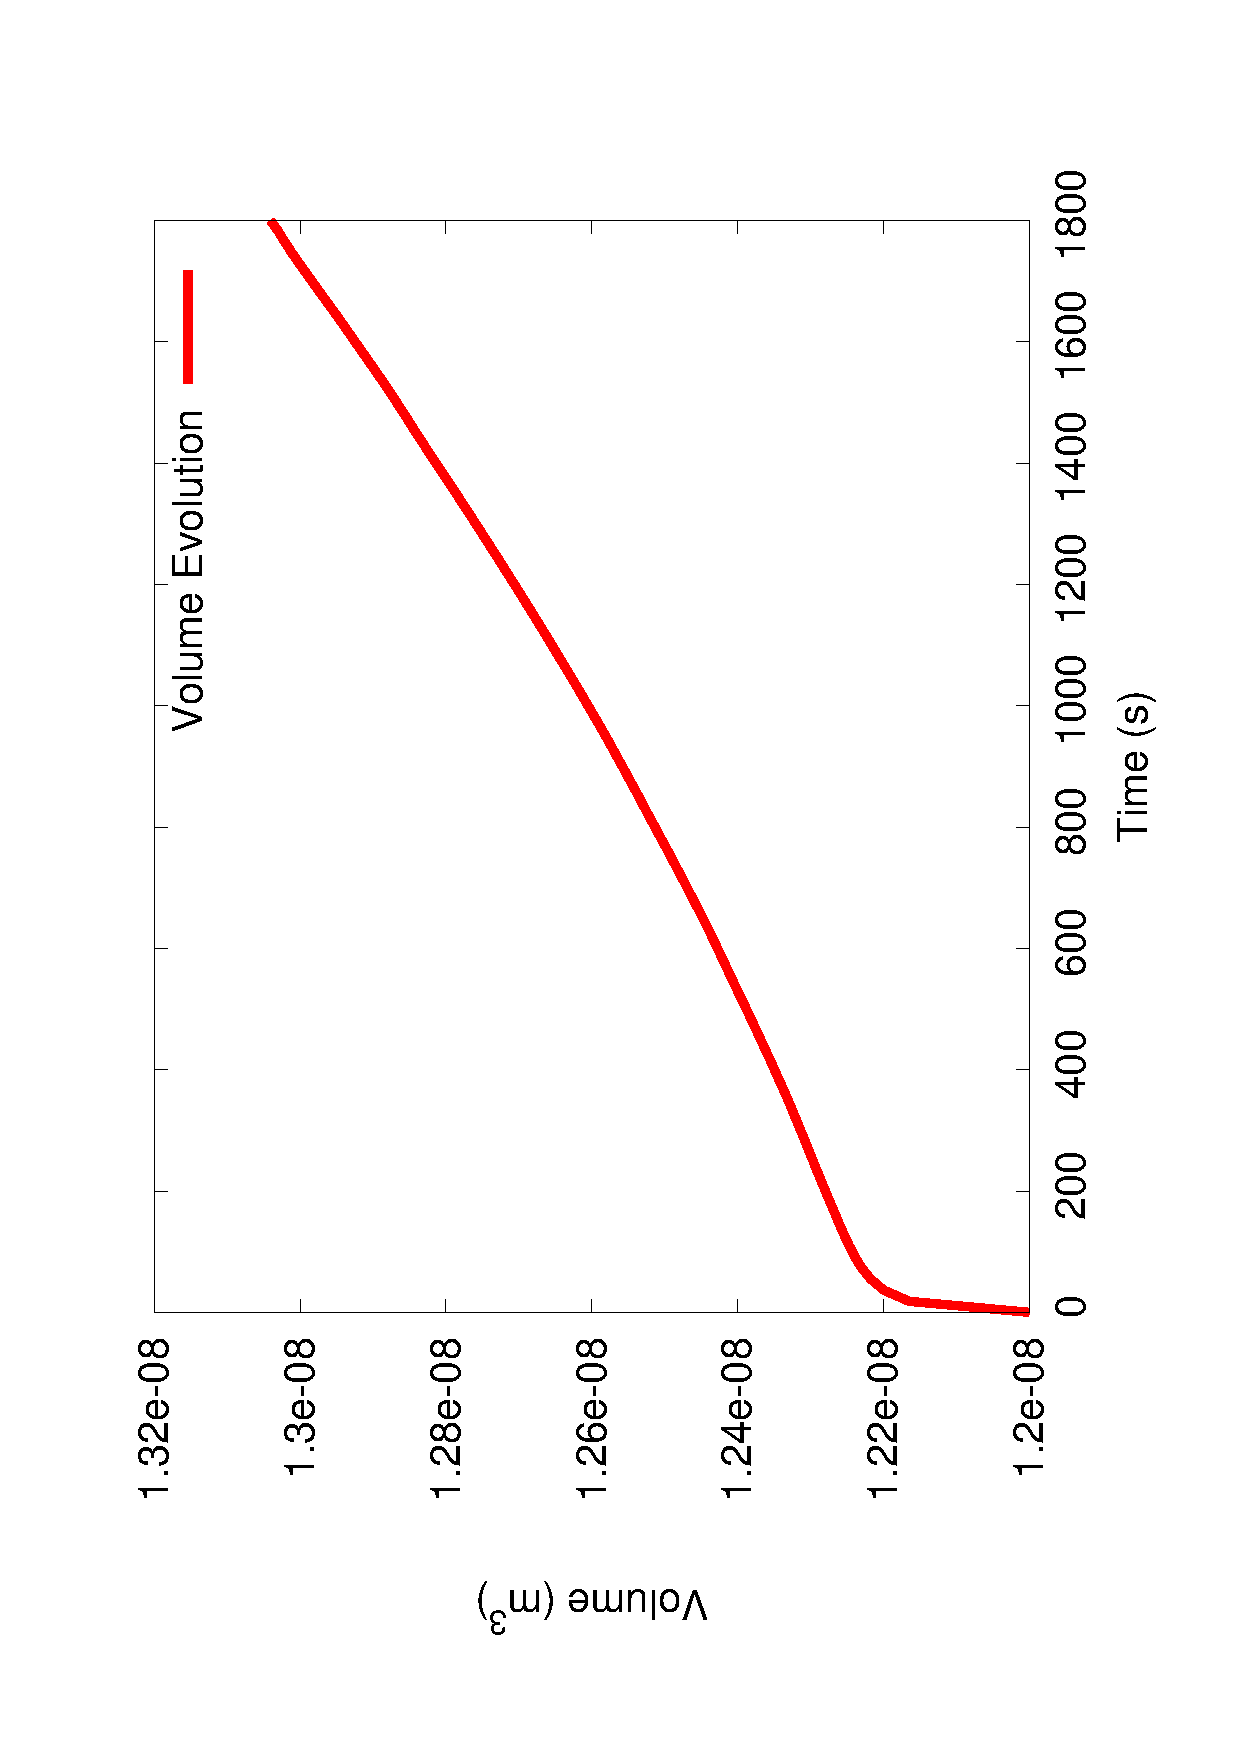
\includegraphics[angle=270,width=0.8\textwidth]{images/examples/lagrangian/swelling/volume-evolution-3}}
     \caption{The volume of the tendon (m$^3$) evolving with
     time. Note the fluid transported-dominated regime until 25 s,
     followed by the longer reaction-dominated growth stage.}
     \label{volume_evolution}
\end{figure}

Motivated mainly by the recognition that the lower bound model for
solid-fluid mechanical coupling ensures convergence to a self-consistent
solution in just a few passes of the staggered solution scheme, we
adopt this version of the coupling for our final problem. On this
  note we point out that solution of the individual balances of linear
  momentum equation for the solid collagenous and fluid phases with
  the momentum transfer terms [$\bq^\mathrm{c}, \bq^\mathrm{f}$ in
  (\ref{linearmombalance})] is a
  statement of momentum balance between them. There is reason to
  suppose, therefore, that equating the solid collagen and fluid
  stress, or some component of these tensors as done in the lower
  bound model, is a reasonable approximation to explicitly solving the
  balance of linear momentum for each phase, including the momentum
  transfers. In contrast, equating the 
  deformation gradient of the solid collagen with deformation of the
  pore spaces subjects the fluid to a stress state also determined by
  this deformation gradient in the upper bound model. This
  approximation does not correspond to an underlying physical
  principle comparable to the satisfaction of individual
  balances of linear momentum for solid collagen and fluid, with
  momentum transfers. It is therefore somewhat less motivated and more
  questionable. Clearly, a rigorous analysis or numerical
  comparisons of all three models:
  upper bound, lower bound and direct solution of individual
  solid-fluid momentum balances, must be carried out to conclusively
  demonstrate this. It is a possible topic for a future paper.

In this example we will demonstrate the mechanical
effects of growth due to collagen production. In the interest of
focusing on this issue we assume that fibroblasts are
available, and that the fluid
phase bears the necessary nutrients for
collagen production dissolved at a suitable, constant
concentration. Collagen production is assumed to be governed by a
first-order rate 
law. Newly-produced collagen has proteoglycan molecules bound to it,
and they in turn bind water. We model this effect by associating a
loss of nutrient-bearing 
free fluid with collagen production. A fluid sink $\Pi^\mathrm{f}$ is
introduced following first order kinetics,

\begin{equation}
\Pi^\mathrm{f} = -k^\mathrm{f}(\rho_0^\mathrm{f}
- \rho_{0_\mathrm{ini}}^\mathrm{f}),
\end{equation}

\noindent as in \citet{growthpaper}. Here $k^\mathrm{f}$ is the
reaction rate, taken to be 0.07 $\mathrm{s}^{-1}$, and
$\rho_{0_\mathrm{ini}}^\mathrm{f}$ is the initial 
concentration of fluid. The collagen
source is mathematically equivalent to the fluid sink: $\Pi^\mathrm{c} =
-\Pi^\mathrm{f}$. When $\rho_{0}^\mathrm{f} >
\rho_{0_\mathrm{ini}}^\mathrm{f}$, collagen is produced.

The boundary conditions in this example correspond to immersion of the
tendon in a nutrient-rich bath. The initial collagen concentration is
500~kg.m$^{-3}$ and the fluid concentration is 400~kg.m$^{-3}$ at
every point in the tendon. When this tendon is exposed to a bath
where the fluid concentration is 410~kg.m$^{-3}$,
i.e. $\rho^\mathrm{f}(\bx,t)=410~\mathrm{kg.m}^{-3} \forall \bx \in
\partial\Omega_t$, nutrient-rich fluid is transported into the tissue,
due to the pressure difference, induced by the concentration
difference, between the fluid in the tendon and in 
the bath (fluid stress gradient-driven flux). Thereby, the nutrient
concentration is elevated, leading to collagen production, fluid
consumption and, eventually, growth due to additional collagen. 

Figure~\ref{before_growth} shows the initial collagen concentration in
the tendon. After it has been immersed in the nutrient-rich bath for
1800~s, the tendon shows growth and the collagen concentration is
higher as seen in Figure~\ref{after_growth}. On performing a
uniaxial tension test on the tendon before and after growth, it is
observed (Figure~\ref{stress_strain}) that the grown tissue is stiffer
and stronger due to its higher collagen concentration. Also note that
there is a rapid, fluid transport-dominated swelling 
of the tendon  between 0 and 25 s 
following immersion in the fluid bath
(Figure~\ref{volume_evolution}). This causes a small volume change of 
$\approx 1.6$\%. In this transport-dominated regime the contribution
to tendon growth from collagen production is small. However, the
fluid-induced swelling saturates, and between
25 and 1800 s the reaction producing collagen dominates the growth
process, producing a further $\approx 6.8$\% volume change. Noting that the
range of collagen concentration in Figure~\ref{after_growth} is
$585-626\; \mbox{kg.m}^{-3}$, and that (\ref{isotropicgrowth}) gives $\bF^{\mathrm{g}^\mathrm{c}} = \left(
  \frac{\rho_0^\mathrm{c}}{\rho_{0_{\mathrm{ini}}}^\mathrm{c}}
  \right)^  {\frac{1}{3}} {\bf 1}$, this portion of the volume change
  is quite clearly due to collagen production. The total volume change
  of $8.4$\% corresponds to changes in each linear dimension of the
  tendon by only $\approx 2.7$\%, and is not discernible upon comparing
  Figures~\ref{before_growth} and \ref{after_growth}. It is, however,
  manifest in Figure~\ref{volume_evolution}.


\begin{figure}[!hpt]
\centering
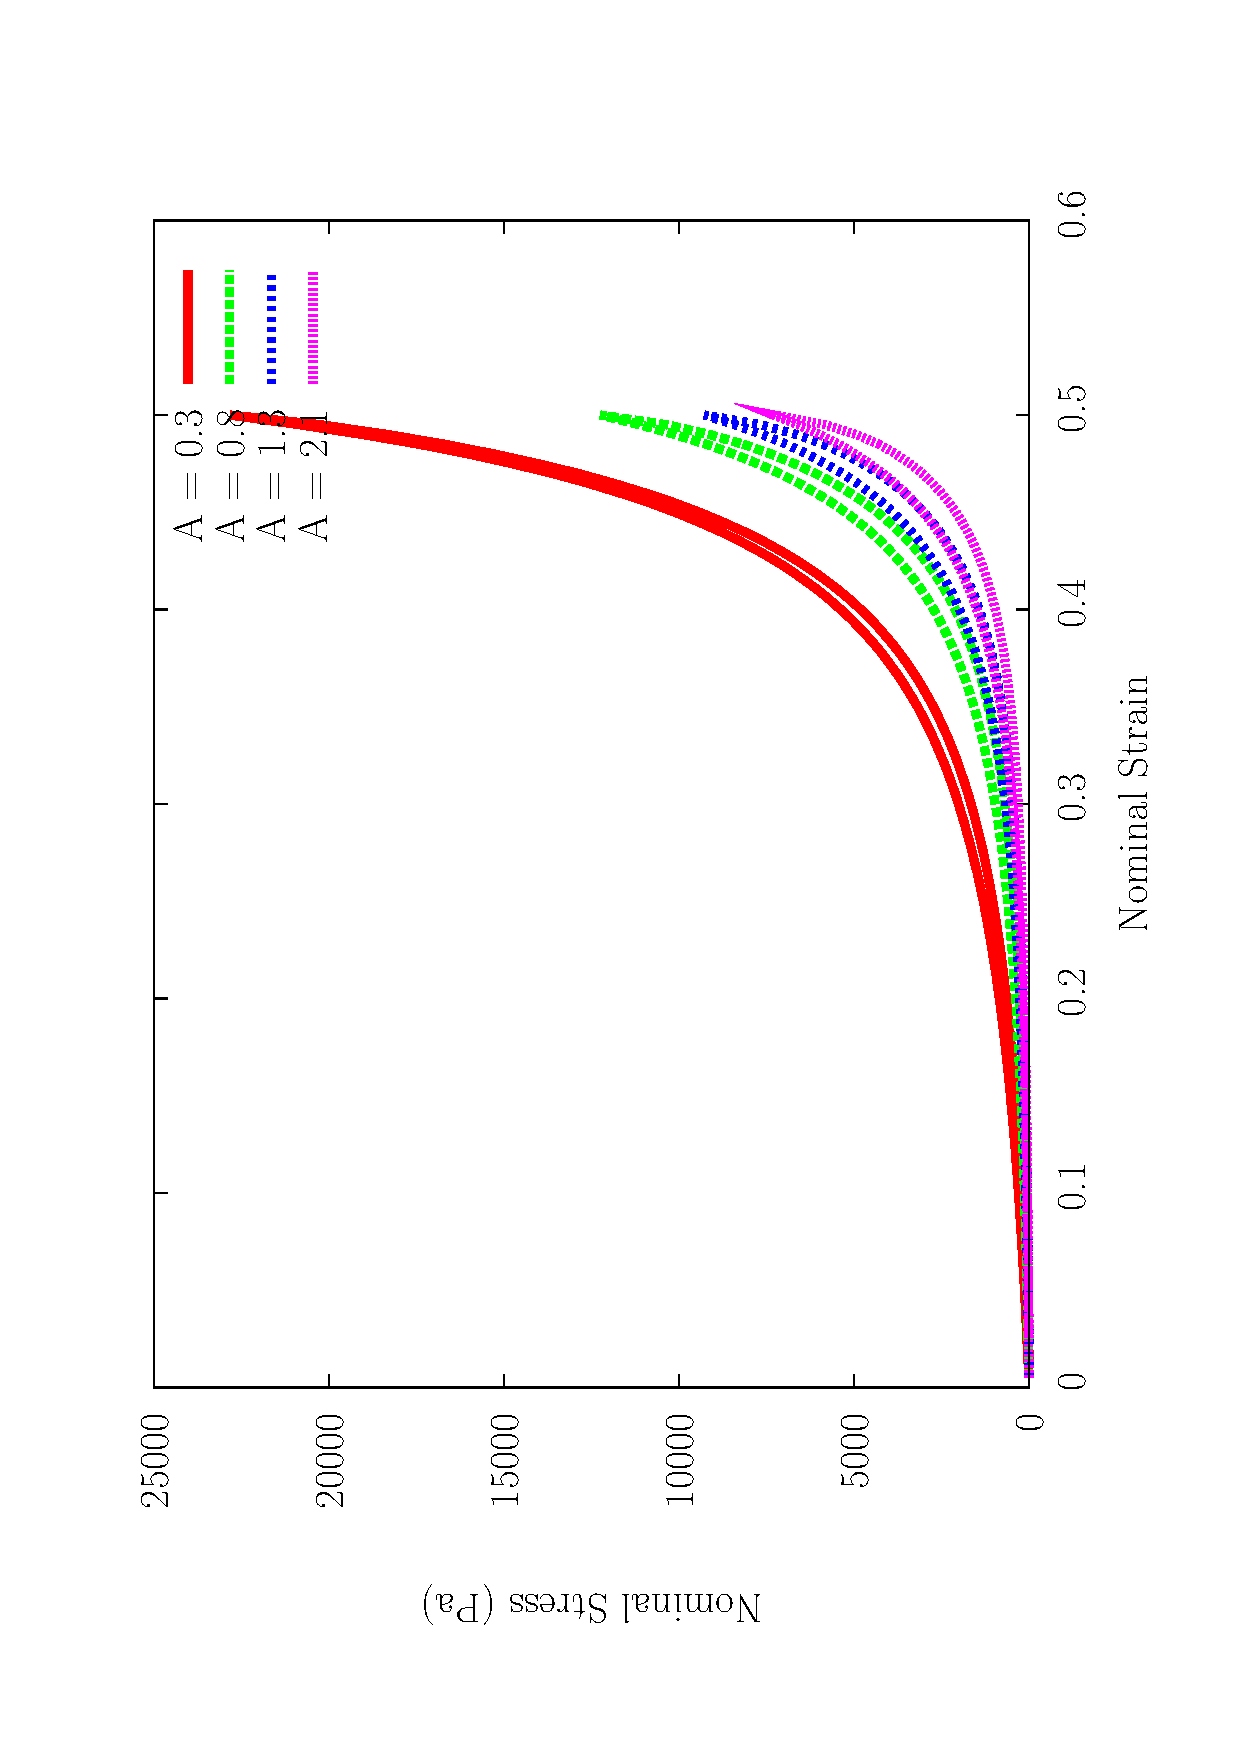
\includegraphics[angle=270,width=0.6\textwidth]{images/examples/lagrangian/cyclic/parametric-study}
\caption{Varying A}
\label{parametric-study}
\end{figure}

\begin{figure}[!hpt]
\centering
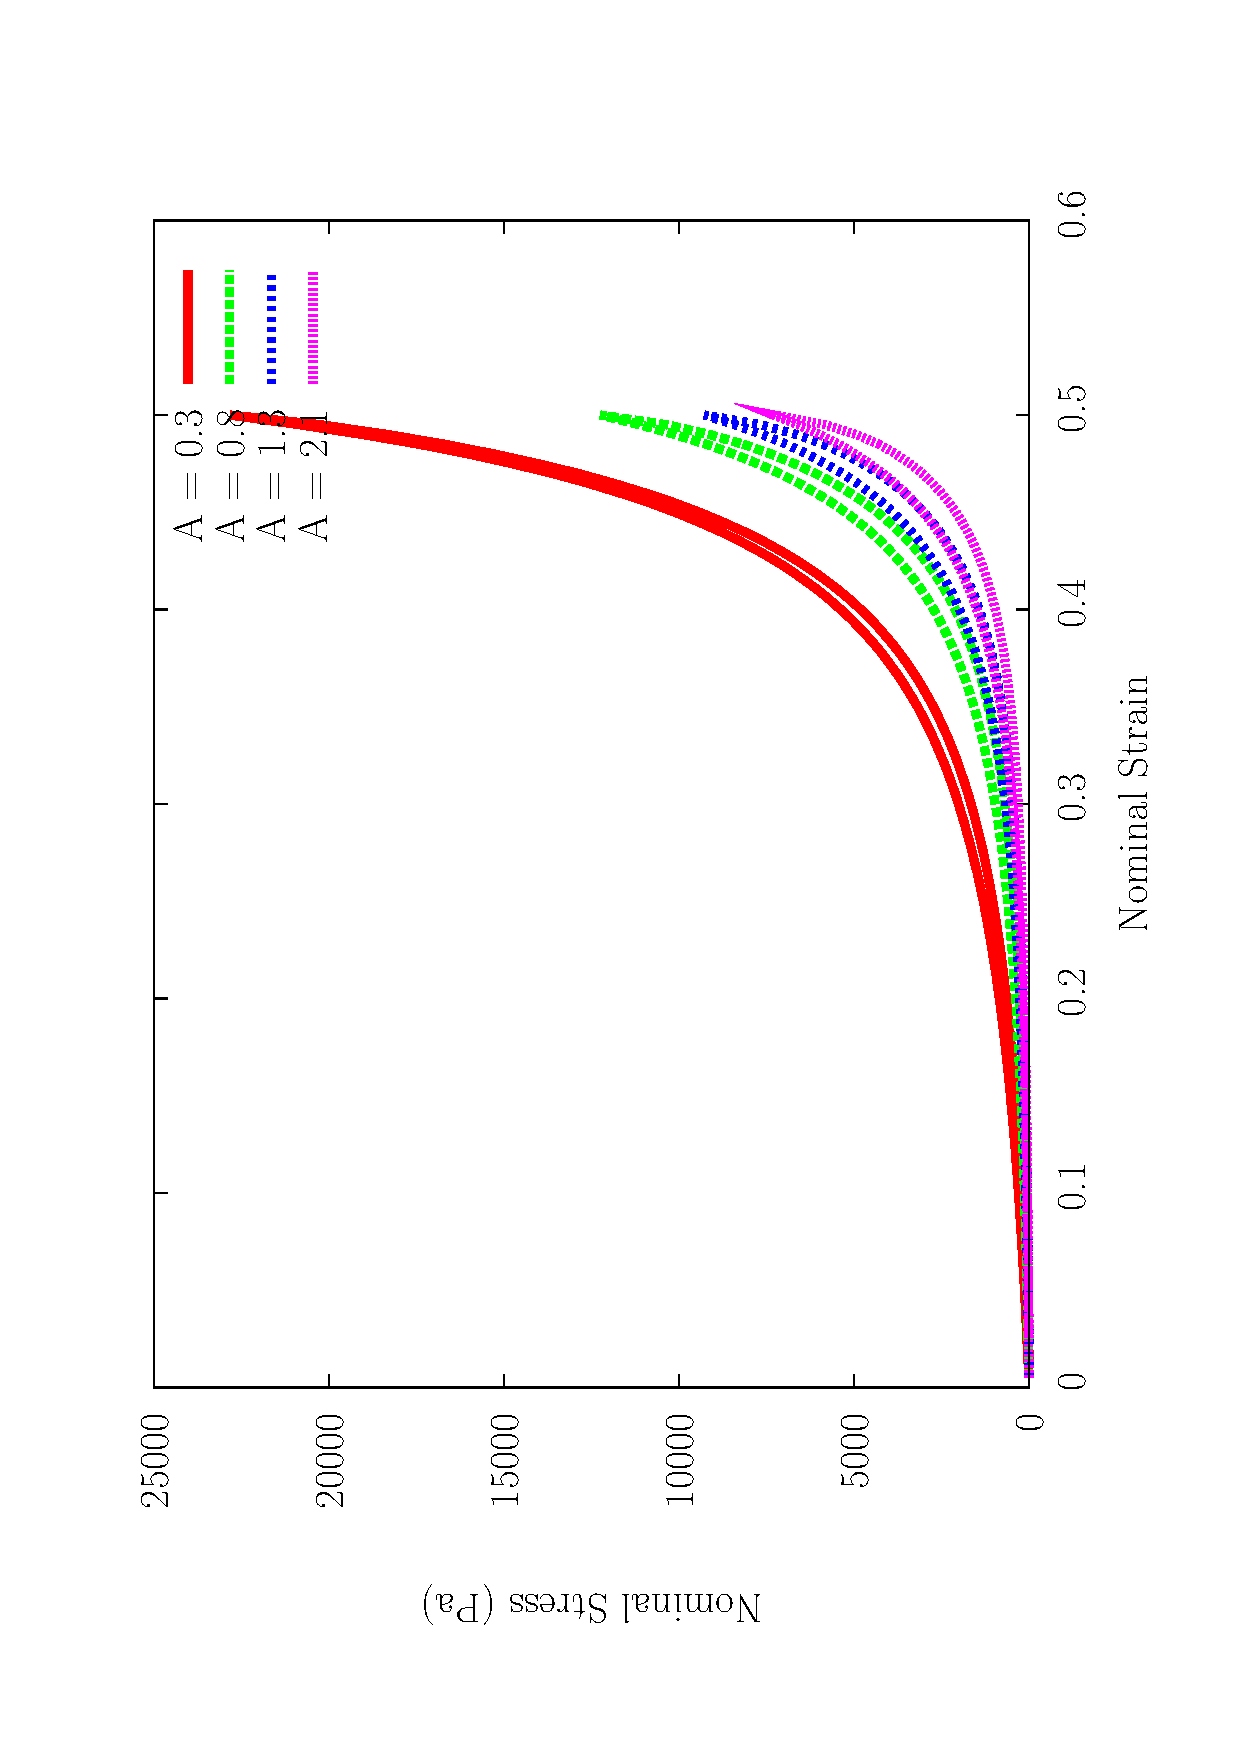
\includegraphics[angle=270,width=0.6\textwidth]{images/examples/lagrangian/cyclic/parametric-study}
\caption{Load-unload cycle}
\label{cyclic-load}
\end{figure}

\section{A multiphasic problem based on enzyme-kinetics}
\label{enzyme-kinetics-example}

\begin{table}
\centering
\begin{tabular}{lll}
\hline
\multicolumn{1}{c}{Parameter (Symbol)} & Value & Units\\
\hline
Chain density ($N$) & $7\times 10^{21}$ & $\mathrm{m}^{-3}$\\
Temperature ($\theta$)  & $310.6$ & K\\
Persistence length ($A$) & $2.10$ & --\\
Fully-stretched length ($L$) & $2.125$ & --\\
Unit cell axes ($a,\;b,\;c$) & $1.95,\;1.95,\;2.43$ & --\\
Bulk compressibility factors ($\gamma,\;\beta$) & $1000,\; 4.5$ & --\\
Fluid bulk modulus ($\kappa^f$) & $1$ & GPa\\
Fluid mobility tensor ($D^\mathrm{f}_{ij} = D^\mathrm{f}\delta_{ij}$) & $1\times 10^{-14}$
&s\\
%Fluid mol. wt. ($\sM^\mathrm{f}$)& $2.991\times 10^{-26}$ & $\mathrm{kg}$\\ 
Fibroblast concentration ($\rho_{\mathrm{cell}}$) & 0.2 &
kg.m$^{-3}$\\
Max. reaction rate ($k_{\mathrm{max}} = 5$) & 5 & s$^{-1}$\\
Max. solute concentration ($\rho^{\mathrm{s}}_m$) & 0.2 &
kg.m$^{-3}$\\
Solute diffusivity ($\bD^\mathrm{s}$) & $1\times 10^{-9}$ &  m$^{-2}$s\\
\hline
\end{tabular}
\caption{Material parameters used in the analysis.}
\label{parameters}
\end{table}

This first example can be viewed as a model for localised, bolus
delivery of regulatory chemicals to the tendon while accounting for
mechanical (stress) effects. A single solute species\footnote{Here, we
  envision the solute to be a protein playing 
  an essential role in growth by catalysing underlying biochemical
  reactions. An important example of this is a family of proteins,
  TGF$\beta$, which is a multi-functional peptide that controls numerous
  functions of many cell types \citep{Alberts:02}.} is considered,
denoted by s, and 
a uniform distribution of fibroblasts that are characterised by their
cell concentration, $\rho_{\mathrm{cell}}$. Both, Fickean diffusion of
the solute, and stress gradient driven fluid flow are incorporated in this
illustration. We use 
Michaelis-Menten enzyme kinetics [Equation~(\ref{enzymekineticseq})]
to determine the rates of solute consumption and collagen production
as a function of solute concentration. This non-linear relationship for
our choice of parameters is visualised in
Figure~\ref{eg3menten}. Here, the fluid phase does not  take part in
reactions, and hence $\Pi^\mathrm{f}=0$. 

\begin{figure}[!hpt]
\centering
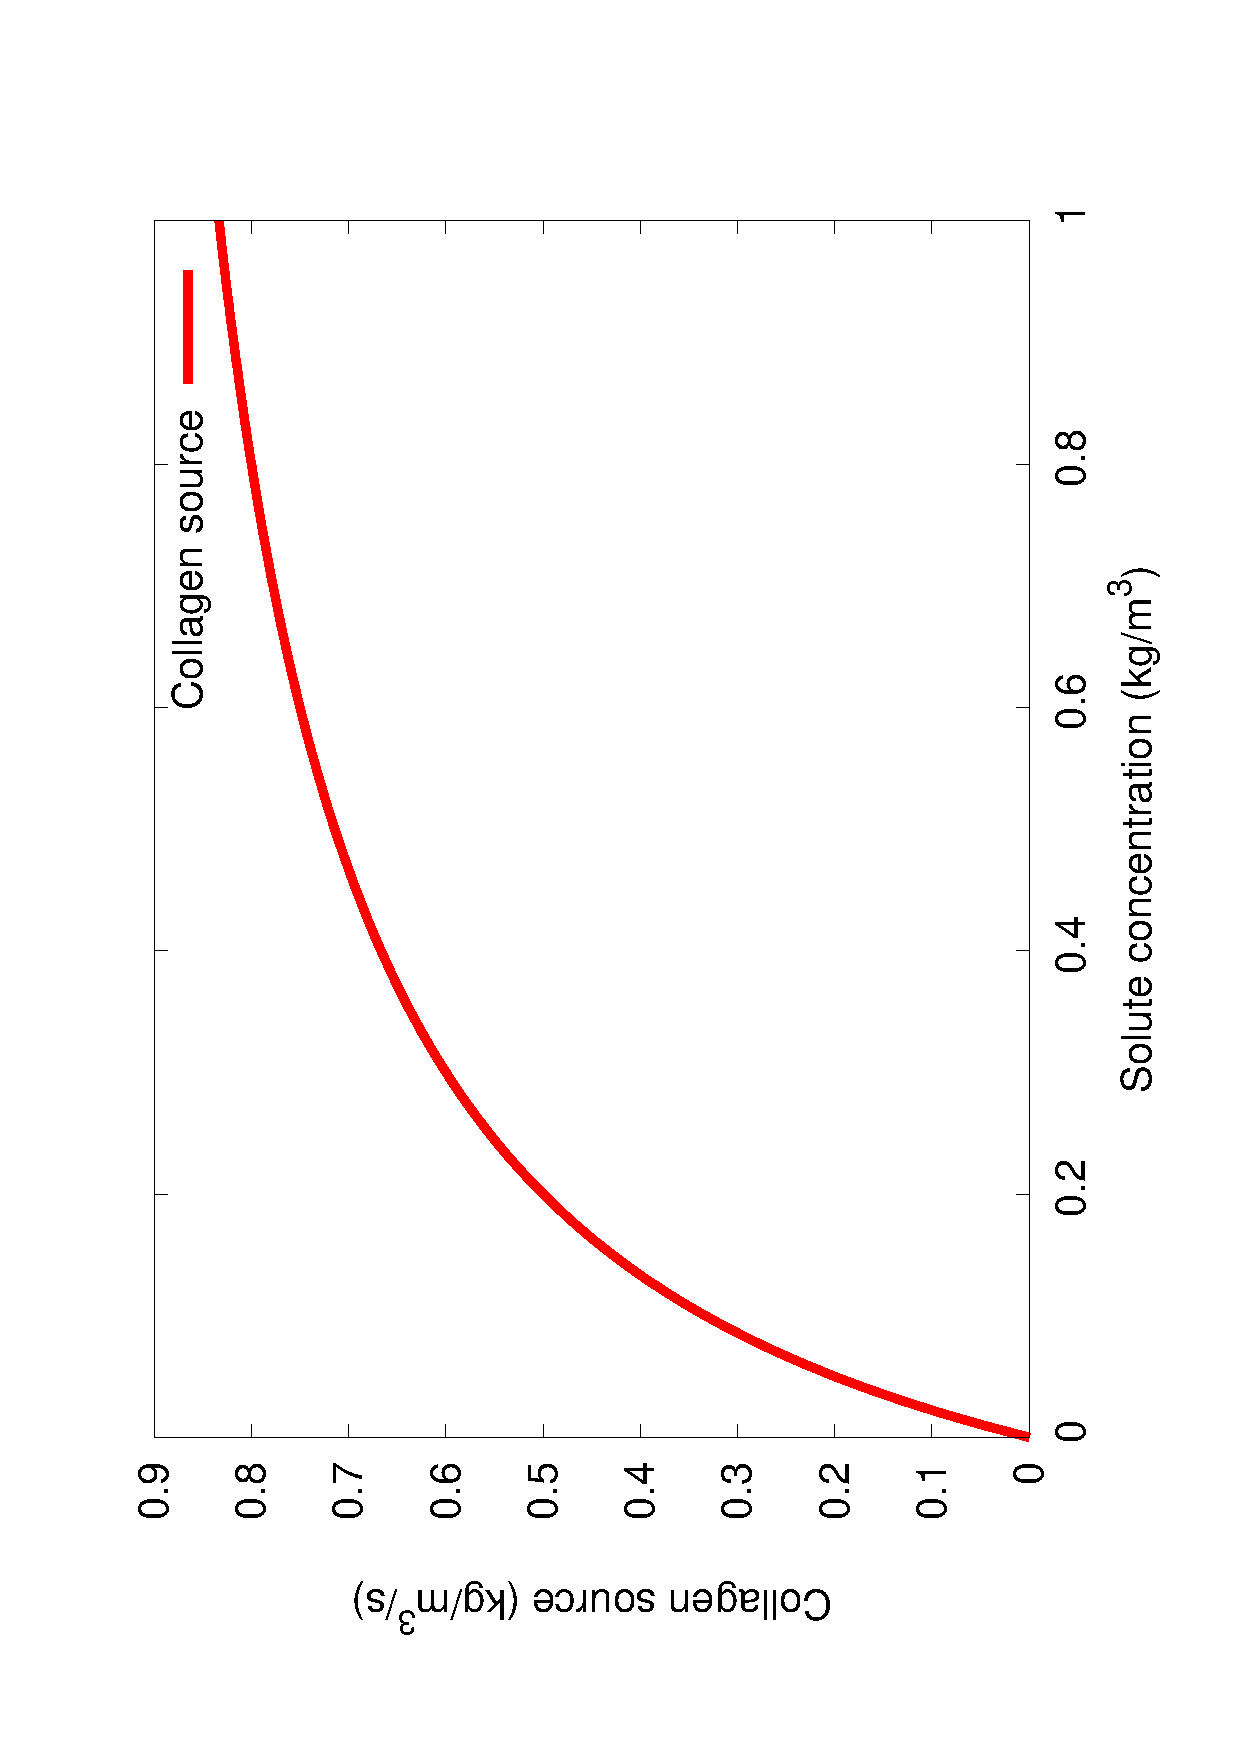
\includegraphics[angle=270,width=0.8\textwidth]{images/elucidation/enzyme-kinetics}
\caption{Variation of the collagen source term (kg.m$^{-3}$.s$^{-1}$)
  with solute concentration (kg.m$^{-3}$).}
\label{eg3menten}
\end{figure}

The tendon immersed in the bath is subjected to a constrictive
radial load, such
as would be imposed upon  manipulating it with a set of tweezers, as depicted in
Figure~\ref{constrictload}. The
maximum strain in the radial 
direction---experienced half-way through the height of the tendon---is
10\%. The applied strain in the radial direction decreases linearly
with distance from the central plane, and vanishes at the top and
bottom surfaces of the tendon. 


\begin{figure}[!hpt]
  \centering
  \psfrag{M}{\small $\bN\cdot\bM^f$}
  \psfrag{P}{\small ${\tiny\quad }~\bu$}
         {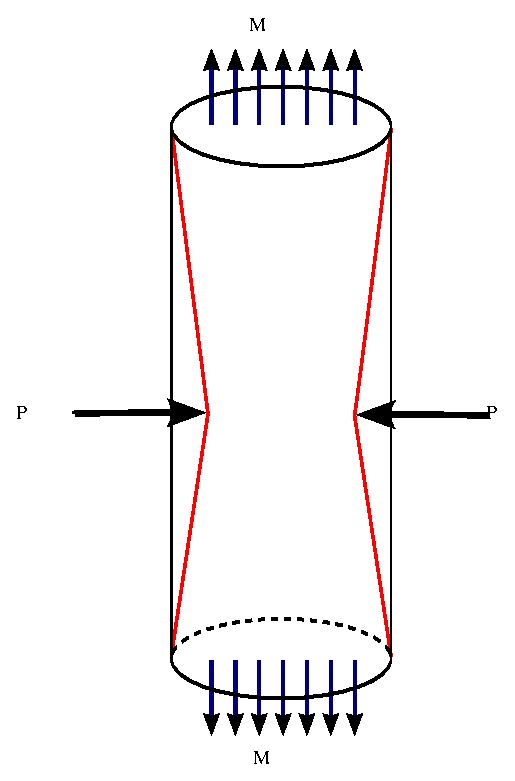
\includegraphics[width=5.0cm]{images/examples/lagrangian/constriction/cylinder-in-bath}}
	 \caption{Constrictive load applied to tendon immersed in a
	 bath.} 
	 \label{constrictload}
\end{figure}

The 
initial collagen concentration and the initial fluid concentration are
both 500~kg.m$^{-3}$ at every point in the tendon, and the fluid
concentration in the bath is 500~kg.m$^{-3}$. In
addition, a solute-rich bulb of radius 0.15~mm is introduced with
its centre on the axis of the tendon and situated 3~mm below the upper
circular face of the tendon. The initial solute concentration is
0.05~kg.m$^{-3}$ at all other points in the tendon, and increases
linearly with decreasing radius in this bulb to 1~kg.m$^{-3}$ at its
centre (see Figure~\ref{eg3ini}). The
parameters used are listed in Table~\ref{parameters}, and are relevant
to tendons.

\begin{figure}[!hpt]
\centering
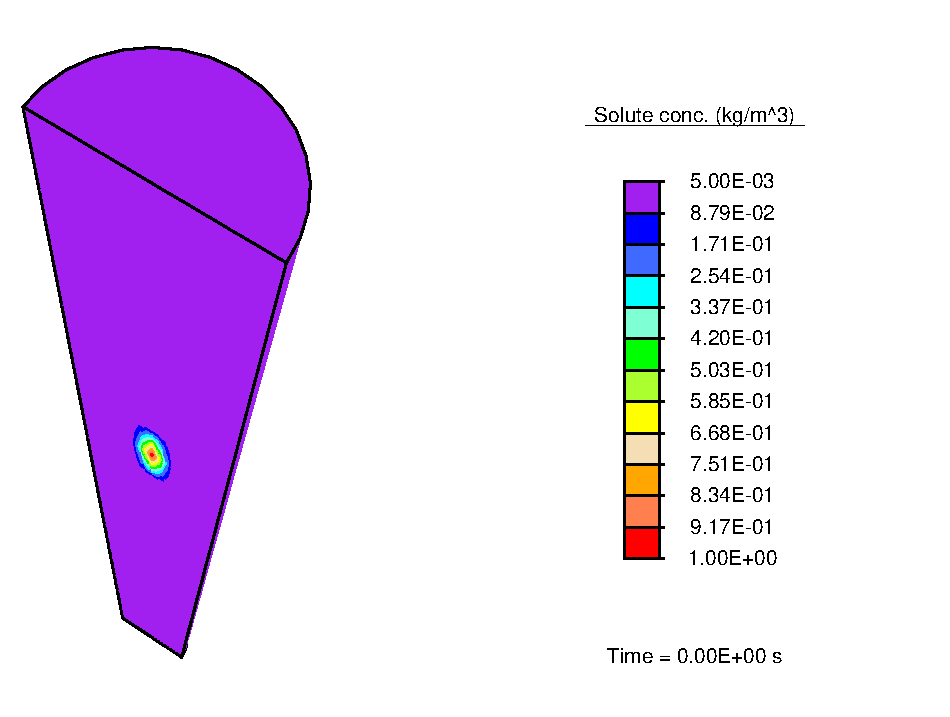
\includegraphics[width=0.8\textwidth]{images/examples/lagrangian/medication/initial-solute-concentration}
\caption{The solute concentration (kg.m$^{-3}$) initially.}
\label{eg3ini}
\end{figure}

The aim of this example is to compare the influences upon solute
transport from two mechanisms: Fluid stress gradient-driven transport,
arising from the applied constrictive load, and solute concentration
gradient-driven transport. These mechanisms have both been implicated
in nutrient supply to cells in soft tissue. The results of this
numerical example demonstrate that because the magnitude of the fluid mobility
for stress gradient driven transport is orders of magnitude
smaller than the diffusion coefficient for the solute through the
fluid, there is relatively only a small stress gradient driven flux,
and the transport of the solute is diffusion dominated. As a result,
the solute diffuses locally, but displays no
observable advection along the fluid. As the diffusion-driven solute
concentration in a region increases, the enzyme-kinetics model
results in a small source term for collagen production, and we observe nominal
growth. Figure~\ref{eg3conc} shows the collagen concentration at an
early time, $t=5\times10^{-2}$~s.

\begin{figure}[!hpt]
\centering
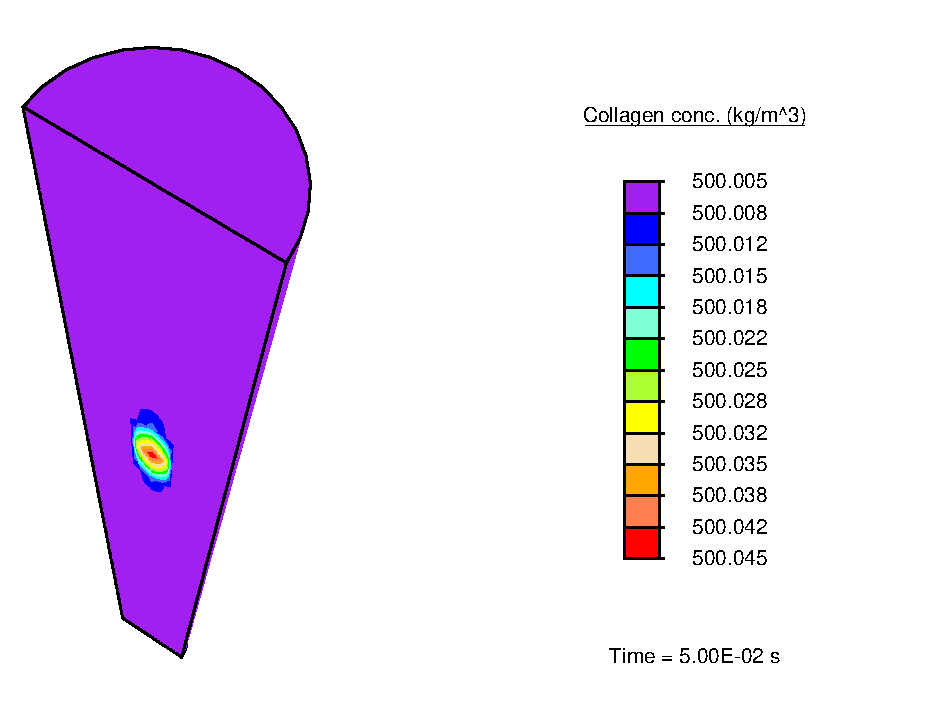
\includegraphics[width=0.8\textwidth]{images/examples/lagrangian/medication/final-collagen-concentration}
\caption{The collagen concentration (kg.m$^{-3}$) at time
  $t=5\times10^{-2}$~s.}
\label{eg3conc}
\end{figure}

This example incorporates all of the theory discussed in the
paper. However, it is a valuable exercise in
modelling to simplify the boundary value problem, and supress some of
the coupled phenomena in order to gain a better understanding of some
effcts. This is the approach followed in the next two numerical
examples. The detailed transport and mechanics induced by the
constrictive radial load are discussed first in Section~\ref{pinching}. 

\section{Extension to modelling wound healing}
\label{wound-healing-example}

%of scars are the result of the body overproducing collagen, which causes the scar to be raised above the surrounding skin. Hypertrophic scars take the form of a red raised lump on the skin, but do not grow beyond the boundaries of the original wound, and they often improve in appearance after a few years

%% chemo-mechanical
%% coupling is described in \cite{Provenzanoetal:2003}.

\begin{figure}[!hpt]
\centering
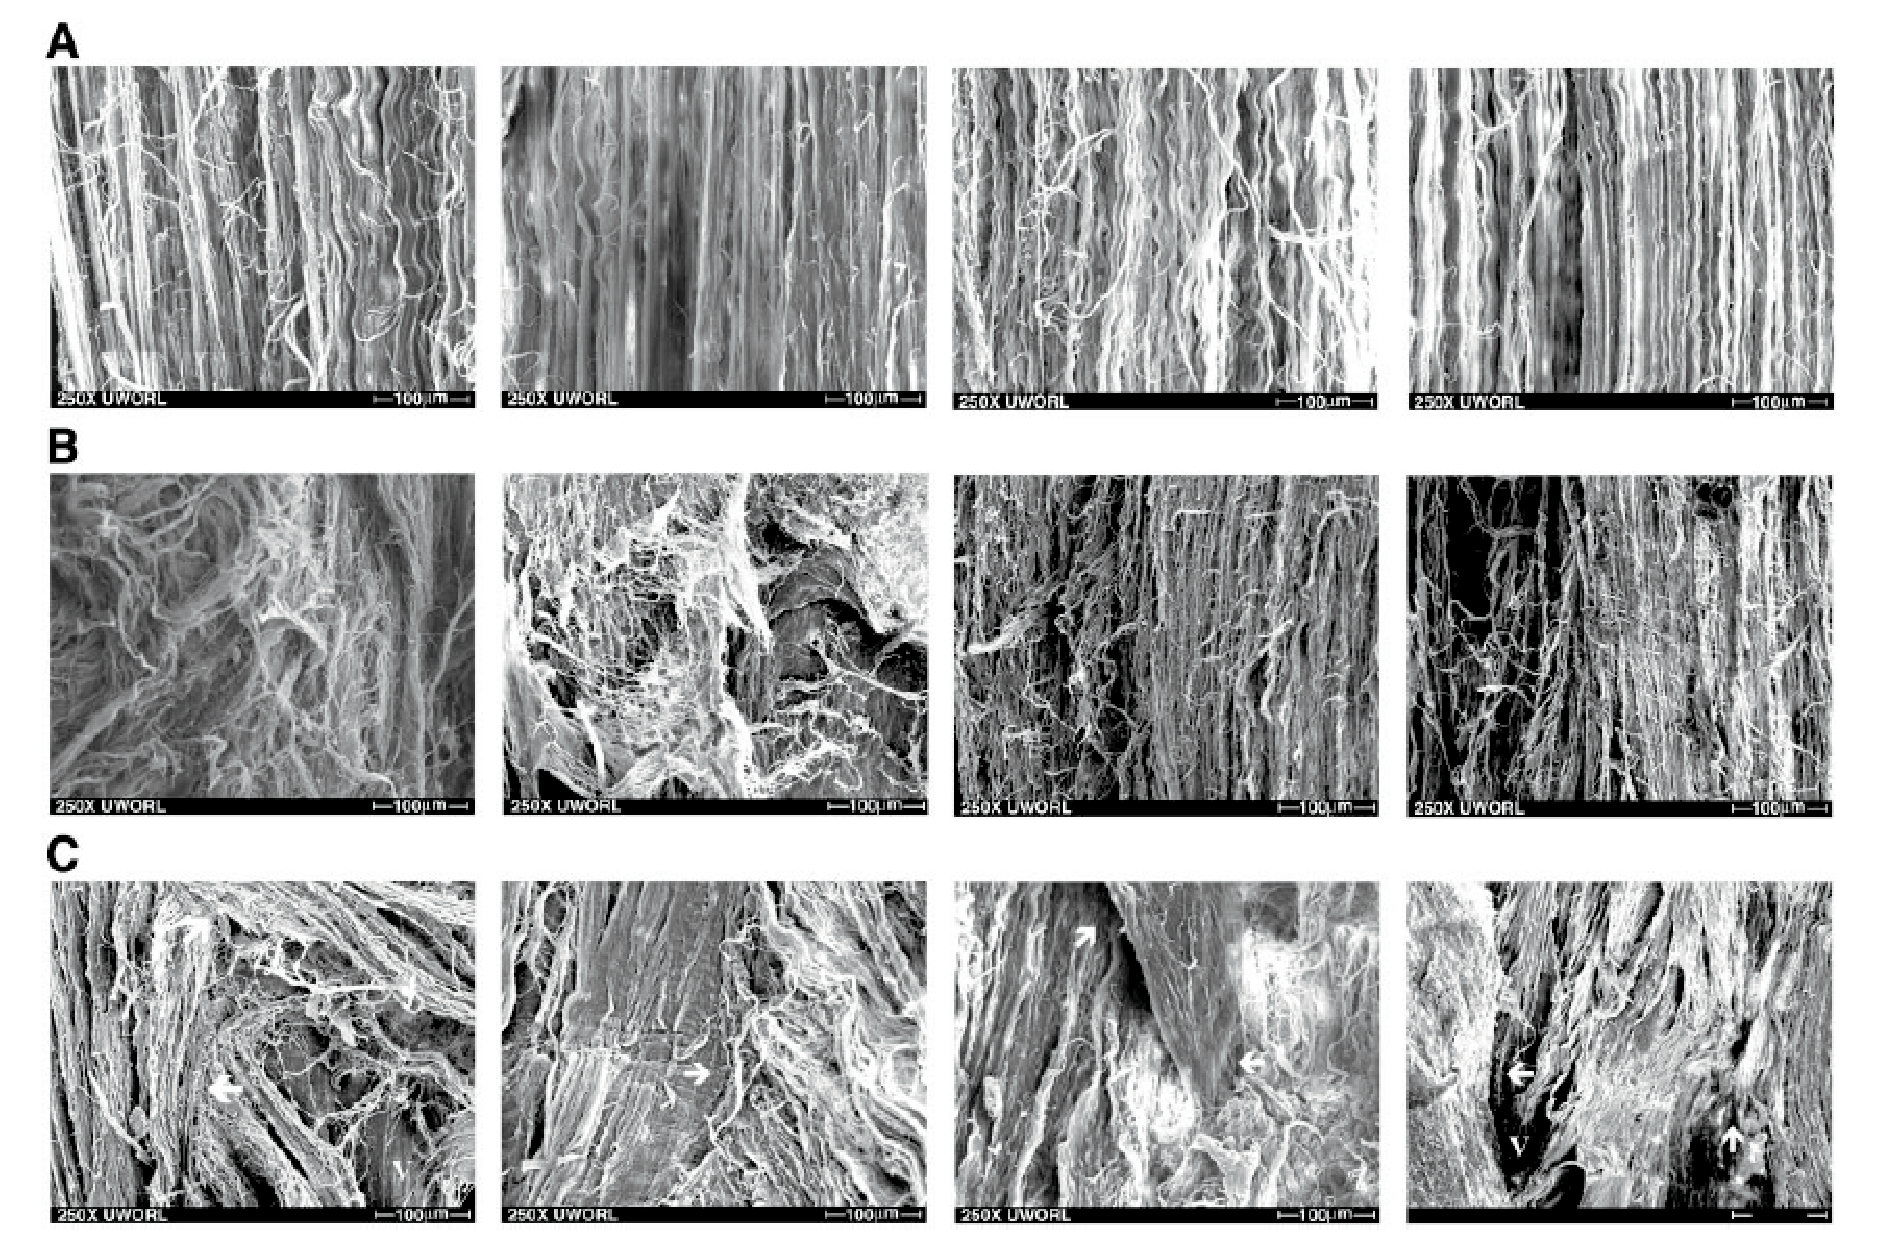
\includegraphics[width=0.8\textwidth]
                {images/experiments/healing-damaged-ligament} 
\caption{The recovery of a damaged ligament.}
\label{healing-damaged-ligament}
\end{figure}

\begin{figure}[!hpt]
\centering
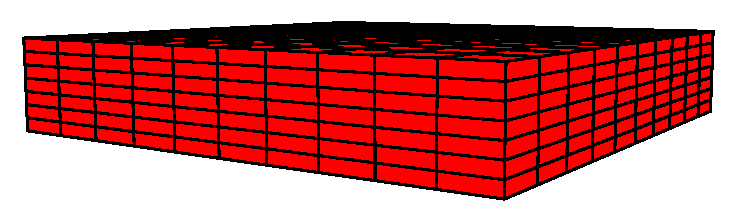
\includegraphics[width=0.8\textwidth]
                {images/examples/lagrangian/healing/full-skin-mesh} 
\caption{The computational mesh representing skin.}
\label{healing-skin-mesh}
\end{figure}

\begin{figure}[!hpt]
\centering
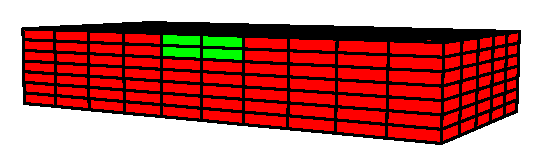
\includegraphics[width=0.8\textwidth]
                {images/examples/lagrangian/healing/damaged-region} 
\caption{The damaged region of the skin highlighted.}
\label{healing-damaged-region}
\end{figure}

\begin{figure}[!hpt]
\centering
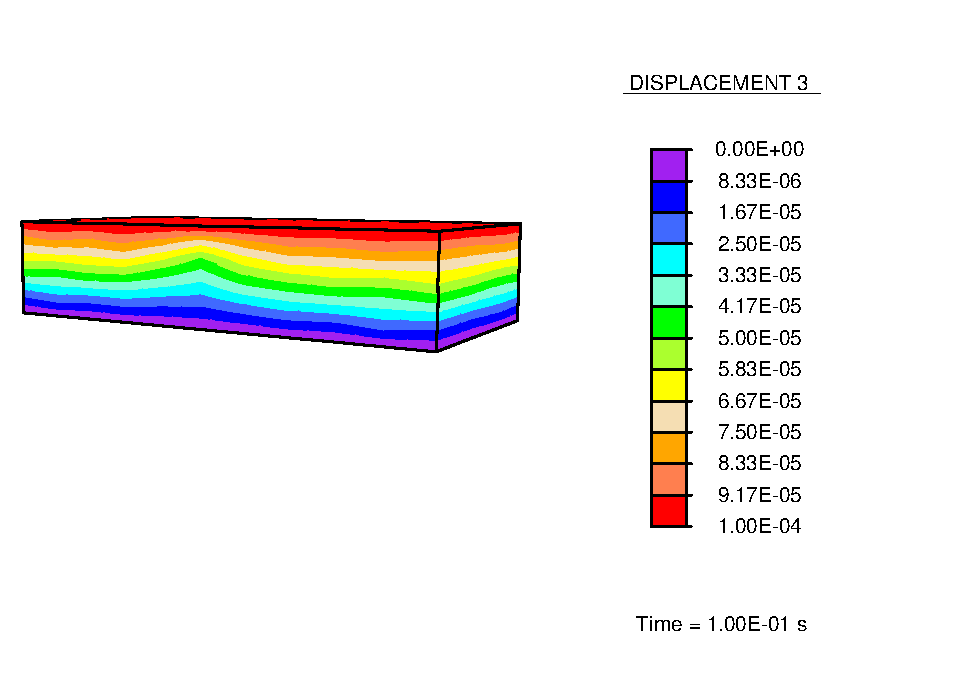
\includegraphics[width=0.8\textwidth]
                {images/examples/lagrangian/healing/healed-vertical-displacement} 
\caption{Vertical displacement upon loading after healing under no external load.}
\label{healing-vertical-displacement}
\end{figure}

\begin{figure}[!hpt]
\centering
\includegraphics[width=0.8\textwidth]
                {images/examples/lagrangian/healing/healed-vertical-stress} 
\caption{Vertical stress upon loading after healing under no external load.}
\label{healing-vertical-stress}
\end{figure}

%% \todo{\begin{itemize}
%%   \item Stronger after growth and mechanics can go here; the tendon
%%     picture can go to the introduction.
%%   \item Needs some literature on the wound healing example; refer
%%     talk10.pdf.
%%   \item Weave around computational details yet again. Point to
%%     established, well known methods of solving the equations and point
%%     to the previous chapter's this-thesis-specific enhancements.
%% \end{itemize}}

%

% Local Variables:
% TeX-master: "thesis"
% mode: latex
% mode: flyspell
% End:

\chapter{An Eulerian perspective}
\label{eulerian-perspective}
\chapter{An Eulerian perspective}
\label{eulerian-perspective}

As detailed at the outset of Chapter~\ref{lagrangian-perspective}, the
continuum treatment presented thus far has stemmed from classical
theories for solid continua, which are traditionally formulated in a
Lagrangian setting. Since our continuum idealisation of tissues
includes fluid components, and material coordinates are, in general,
not known in fluid mechanics, this chapter revisits the derivation of
the governing field equations of growing tissues following an Eulerian
approach.

In this {\em spatial description}, attention is turned to a region of
space coinciding with the {\em current configuration} of the tissue,
where the evolution of field variables of interest are
studied. Remarkably, this dissimilar approach results in a set of
balance equations which are completely equivalent to those deduced in
Section~\ref{balance-laws}, just {\em pushed-forward} to the current
configuration. But more significantly, the spatial approach presented
below naturally leads to the identification of a different set of
primitive variables more suitable to physically relevant boundary
value problems.

This chapter is divided into two main parts. The first part
(Section~\ref{eu-balance-laws}) briefly recapitulates the fundamental
quantities characterising the tissue, pointing out noteworthy
differences from Section~\ref{balance-laws}, and derives the balance
laws governing finite deformation growth in terms of spatial
quantities. The second (Section~\ref{eu-entropy-inequality}), closes
this set of balance laws by deducing a set of physiologically relevant
constitutive relationships which ensure that the entropy inequality is
satisfied a priori.

\section{Balance laws for an open mixture}
\label{eu-balance-laws}

We initiate this discussion with the introduction of $\Omega_{t}$, a
temporally-varying closure of an open set in $\mathbb{R}^{3}$ with a
piecewise smooth boundary, which we define to be our region of
interest. This region of interest is constructed to coincide with the
current position of the solid component of the tissue, and our primary
interest lies in the evolution of various field variables inside
$\Omega_{t}$, as observed from an inertial reference frame
(\citet{newton1726}, Corollary~V, p.~423).

\begin{figure}
  \centering
  \psfrag{A}{$\bX$}
  \psfrag{B}{$\Omega_0$}
  \psfrag{C}{$\Bvarphi_{t}$}
  \psfrag{D}{$\bx$}
  \psfrag{E}{$\Omega_t$}
  \psfrag{F}{$\bX^{\iota}$}
  \psfrag{G}{$\Omega_{0}^{\iota}$}
  \psfrag{H}{$\Bvarphi^{\iota}_{t}$}
  \includegraphics[width=0.8\textwidth]{images/elucidation/%
    continuum-potato-current-configuration}
  \caption{An Eulerian point of view.}
  \label{continuum-potato-current-configuration}
\end{figure}

It is assumed that the there exists a {$\mathit{C}^{2}$} (in space and
time), bijective and orientation preserving map $\Bvarphi_{t}(\bX):
\mathbb{R}^3\times\mathbb{R}^{+}\cup\{0\} \rightarrow\mathbb{R}^{3}$
such that $\Omega_{t} = \Bvarphi_{t} (\Omega_{0})$ for some
convenient, {\em fixed} subset of $\mathbb{R}^{3}$, $\Omega_{0}$. This
ensures that $\Omega_{t}$ evolves in a well-behaved manner,
disallowing non-physical deformations from being imposed on the
tissue, and furthermore, affords the application of Reynolds'
Transport Theorem (Appendix~\ref{reynolds-transport}). The map
$\Bvarphi_{t}$ is visualised in Figure~\ref{continuum-potato%
-current-configuration}.

Denoting a point in $\Omega_{t}$ by $\bx$, $\bv(\bx,t) =
\frac{\partial \Bvarphi_{t}}{\partial t}$ defines the {\em spatial
  velocity} of the system domain. In contrast to
Section~\ref{balance-laws}, it is recognised at the outset that each
species of the tissue is capable of undergoing its own motion
independent of the tissue's solid component; and so we introduce the
spatial velocity of an arbitrary species~$\iota$,
$\bv^{\iota}(\bx,t)$, which is assumed to be $\mathit{C}^{1}$ in space
and time.\footnote{It is important to note that these quantities are
  primitive variables in themselves. While these species velocities
  can be formally understood as \mbox{$\bv^{\iota}(\bx,t) =
    \frac{\partial \Bvarphi^{\iota}_{t}}{\partial t}$}, where
  $\Bvarphi^{\iota}_{t}$ is the deformation map of each
  species~$\iota$ from an arbitrary reference configuration to
  $\Omega_{t}$ (shown in the portion of Figure~\ref{continuum-potato%
    -current-configuration} constructed using dashed-lines), the
  quantities $\Bvarphi^{\iota}_{t}$ are neither explicitly defined nor
  tracked.}  Unlike the corresponding quantities defined in
Section~\ref{balance-of-linear-momentum}, these velocities are defined
to be the {\em total} velocities of each species, not velocities
relative to the solid component of the tissue.\footnote{And, with the
  redefinition of these quantities as total velocities, the velocity
  of the solid phase ceases to be special. This is manifest in the
  forms of the balance laws deduced in Sections~\ref{eu-balance-of%
    -mass}--\ref{eu-balance-of-energy}.}

The following discussion of balance laws is carried out entirely in
terms of an arbitrary species~$\iota$, and specialisation to the solid
collagenous, fluid and solute phases (i.e. \mbox{$\iota=\mathrm{c},
  \mathrm{f}, \mathrm{s}$}) is reintroduced only in Section~\ref{eu%
  -entropy-inequality} when discussing constitutive relationships
specific to these different components of the tissue.

\subsection{Balance of mass}
\label{eu-balance-of-mass}

We now turn our attention to the evolution of the first of our field
variables of interest, the current concentration of an arbitrary
species~$\iota$ constituting the system, $\rho^{\iota}(\bx,t):
\mathbb{R}^3\times\mathbb{R}^{+}\cup\{0\} \rightarrow
\mathbb{R}$. These are defined as the mass of species~$\iota$ per unit
       {\em system volume}, $\Omega_{t}$, and are assumed to be
       $\mathit{C}^{1}$ in time and $\mathit{C}^{2}$ in space. The
       total {\em spatial density} of the tissue can be obtained by
       their summation, $\sum\limits_{\iota}\rho^\iota = \rho$.

With these quantities defined, we have from the conservation of matter
for species $\iota$ over $\Omega_{t}$,

\begin{equation}
\underbrace{\frac{\mathrm{d}} {\mathrm{d}t}\left(\int_{\Omega_{t}}
  \rho^{\iota} \ \mathrm{d}v \right)}_{\text{Rate of change of mass}}
= \underbrace{\int_{\Omega_{t}} \pi^{\iota} \ \mathrm{d}v}_{\text{Mass
    being created}} - \underbrace{\int_{\partial \Omega_{t}}
  \rho^{\iota} \left(\bv^{\iota} - \bv\right) \cdot
  \bn\ \mathrm{d}a,}_{\text{Mass leaving the domain}}
\label{eu-globalbalanceofmass}
\end{equation}

\noindent where $\pi^{\iota}(\bx,t)$ is the volumetric source (or
sink) of species~$\iota$, which specifies the species' mass production
rate per unit system volume, and $\bn$ is the outward normal vector
over $\partial \Omega_{t}$, the boundary of $\Omega_{t}$. At this
point, the only restriction on the source terms, $\pi^{\iota}(\bx,t)$,
is that they be integrable.

On applying Reynolds' Transport Theorem
(Appendix~\ref{reynolds-transport}) to the left hand-side,

\begin{equation*}
\int_{\Omega_{t}} \frac{\partial \rho^{\iota}}{\partial t}
\ \mathrm{d}v + \cancel{\int_{\partial \Omega_{t}} \rho^{\iota} \bv
  \cdot \bn\ \mathrm{d}a} = \int_{\Omega_{t}} \pi^{\iota}
\ \mathrm{d}v - \int_{\partial \Omega_{t}} \rho^{\iota}
\left(\bv^{\iota} - \cancel{\bv}\right) \cdot \bn\ \mathrm{d}a,
\end{equation*}

\noindent Gauss' Divergence Theorem (Appendix~\ref{gauss-divergence})
to the area integral,

\begin{equation*}
\int_{\Omega_{t}} \frac{\partial \rho^{\iota}}{\partial t}
\ \mathrm{d}v = \int_{\Omega_{t}} \pi^{\iota} \ \mathrm{d}v -
\int_{\Omega_{t}} \mathrm{div} \left( \rho^{\iota} \bv^{\iota}\right)
\ \mathrm{d}v,
\end{equation*}

\noindent and localising, we arrive at the final form of the balance
of mass of species $\iota$,

\begin{equation}
\frac{\partial \rho^{\iota}}{\partial t} = \pi^{\iota} -\ \mathrm{div}
\left(\rho^{\iota} \bv^{\iota}\right) \quad \mathrm{in}\ \Omega_{t},
\label{eu-localbalanceofmass}
\end{equation}

\noindent where $\mathrm{div} (\bullet)$ denotes the spatial
divergence operator. This result is consistent with classical mixture
theory \citep{TruesdellToupin:60} and is the current configuration
analogue of Equation~(\ref{localbalanceofmass}).

As in Section~\ref{balance-of-mass}, recall that for an external
observer, the rate of change of mass of the entire system, affected
only by external agents, is independent of interconversion between
species. From the viewpoint of such an observer, the balance of mass
for the tissue as a whole reads,

\begin{equation}
\frac{\mathrm{\mathrm{d}}}{\mathrm{\mathrm{d}}t} \sum\limits_{\iota}
\left(\int_{\Omega_{t}} \rho^{\iota} \ \mathrm{d}v \right) =
-\sum\limits_{\iota} \int_{\partial \Omega_{t}} \rho^{\iota}
\left(\bv^{\iota} - \bv\right) \cdot \bn\ \mathrm{d}a.
\label{eu-systembalanceofmass}
\end{equation}

\noindent Comparing Equation~(\ref{eu-systembalanceofmass}) to a
summation of Equation~(\ref{eu-globalbalanceofmass}) over all species,
both being valid statements of the balance of mass of the tissue as a
whole, it is clear that the sources and sinks satisfy,

\begin{equation}
\sum\limits_{\iota}\pi^{\iota} = 0.
\label{eu-summationrelationmass}
\end{equation}

\noindent In words, the above relation states that the only kinds of
chemical interactions considered in the formulation are those in which
the masses of species get interconverted between each other, i.e.,
the system contains no internal sources of matter.

An identical relation is obtained by \citet{TruesdellToupin:60} and
others who follow their ideas (see, for e.g., \citet{bowen76} and
\citet{passmanetal}), but their deduction of
this result, and other similar results involving quantities internal
to the system (Equations~(\ref{eu-summationrelationmomentum}) and
(\ref{eu-summationrelationenergy})), stems from a formally stated
assumption that ``the mean response of a heterogeneous mixture obeys
the ordinary equations of a continuum.'' While we do not explicitly
employ this assumption, it is implicit in our assertion that external
observers can quantify field variables characterising species within a
system without being aware of phenomena internal to the system.

\subsection{The balance of linear momentum}
\label{eu-balance-of-linear-momentum}

We now look at how the momentum of a species evolves under the action
of external agents, accounting for mass sources and allowing for the
possibility that matter can leave the domain.

As observed from an inertial reference frame, the balance of momentum
of a species~$\iota$ over $\Omega_{t}$ requires,

\begin{equation}
\begin{split}
\underbrace{\frac{\mathrm{d}}{\mathrm{d}t}\left(\int_{\Omega_{t}}
  \rho^{\iota} \bv^{\iota}\ \mathrm{d}v \right)}_{\text{Rate of change
    of momentum}} = & \underbrace{\int_{\Omega_{t}} \rho^{\iota}
  \left(\bg^{\iota} +
  \bq^{\iota}\right)\ \mathrm{d}v}_{\text{Resultant body force}} +
\underbrace{\int_{\partial \Omega_{t}}
  \Bsigma^{\iota}\bn\ \mathrm{d}a}_{\text{Boundary traction}}\\ + &
\underbrace{\int_{\Omega_{t}}
  \pi^{\iota}\bv^{\iota}\ \mathrm{d}v}_{\text{Momentum being created}}
- \underbrace{\int_{\partial \Omega_{t}} \left(\rho^{\iota}
  \bv^{\iota} \right) \left(\bv^{\iota} - \bv\right) \cdot
  \bn\ \mathrm{d}a,}_{\text{Momentum leaving the domain}}
\end{split}
\label{eu-globalbalanceofmomentum}
\end{equation}

\noindent where, in addition to the quantities introduced previously,
$\bg^{\iota}(\bx,t)$ is the resultant body force of {\em external}
origin acting on species $\iota$, $\bq^{\iota}(\bx,t)$ is the
resultant body force on species $\iota$ from all other species {\em in
  the mixture}, and $\Bsigma^{\iota}(\bx,t)$ is the partial Cauchy
stress on species $\iota$. The partial Cauchy stress tensor
corresponding to species~$\iota$ is the portion of the total stress
borne by the species. All of these quantities are assumed to be
sufficiently smooth. In particular, $\bg^{\iota}$ and $\bq^{\iota}$
are assumed to be integrable, and $\Bsigma^{\iota}$ is assumed to be
$\mathit{C}^{1}$ in space and time.

Application of Reynolds' Transport Theorem (Appendix~\ref{reynolds%
  -transport}) to the left hand-side of Equation~(\ref{eu-%
  globalbalanceofmomentum}) yields,

\begin{equation*}
\begin{split}
\int_{\Omega_{t}} \frac{\partial
  \left(\rho^{\iota}\bv^{\iota}\right)}{\partial t} \ \mathrm{d}v
+\cancel{\int_{\partial \Omega_{t}}
  \left(\rho^{\iota}\bv^{\iota}\right) \bv \cdot \bn\ \mathrm{d}a} = &
\int_{\Omega_{t}} \rho^{\iota} \left(\bg^{\iota}+\bq^{\iota}\right)
\ \mathrm{d}v + \int_{\partial \Omega_{t}}
\Bsigma^{\iota}\bn\ \mathrm{d}a\\ + & \int_{\Omega_{t}}
\pi^{\iota}\bv^{\iota} \ \mathrm{d}v - \int_{\partial \Omega_{t}}
\left(\rho^{\iota} \bv^{\iota} \right)\left(\bv^{\iota} -
\cancel{\bv}\right) \cdot \bn\ \mathrm{d}a.
\end{split}
\end{equation*}

\noindent Using the product rule, Gauss' Divergence Theorem
(Appendix~\ref{gauss-divergence}), and the balance of
mass{\footnote{Recognising that the balance of mass need not be
    satisfied exactly, pointwise in a numerical implementation.}}
(Equation~\ref{eu-localbalanceofmass}), we have,

\begin{equation*}
\begin{split}
\cancel{\int_{\Omega_{t}} \frac{\partial \rho^{\iota}} {\partial t}
  \bv^{\iota} \ \mathrm{d}v} + \int_{\Omega_{t}} \rho^{\iota}
\frac{\partial \bv^{\iota}} {\partial t} \ \mathrm{d}v = &
\int_{\Omega_{t}} \rho^{\iota} \left(\bg^{\iota}+\bq^{\iota}\right)
\ \mathrm{d}v + \int_{\Omega_{t}}
\mathrm{div}\left(\Bsigma^{\iota}\right)\ \mathrm{d}v\\ + &
\cancel{\int_{\Omega_{t}} \pi^{\iota}\bv^{\iota} \ \mathrm{d}v} -
\int_{\Omega_{t}}\left(\cancel{\mathrm{div}
  \left(\rho^{\iota}\bv^{\iota}\right) \bv^{\iota}} +
\mathrm{grad}\left(\bv^{\iota}\right)
\rho^{\iota}\bv^{\iota}\right)\ \mathrm{d}v,
\end{split}
\end{equation*}

\noindent where $\mathrm{grad} (\bullet)$ denotes the spatial gradient
operator. Upon localisation, we obtain the final form of the balance
of momentum of species $\iota$,

\begin{equation}
\rho^{\iota} \frac{\partial \bv^{\iota}} {\partial t} = \rho^{\iota}
\left(\bg^{\iota}+\bq^{\iota}\right) +
\mathrm{div}\left(\Bsigma^{\iota}\right) -
\mathrm{grad}\left(\bv^{\iota}\right) \rho^{\iota}\bv^{\iota} \quad
\mathrm{in}\ \Omega_{t},
\label{eu-localbalanceofmomentum}
\end{equation}

\noindent which is a result consistent with classical mixture theory
\citep{TruesdellToupin:60} and is current configuration analogue of
Equation~(\ref{localbalanceofmomentum}).

Neglecting the interaction terms as an external observer, the balance
of momentum for the entire system can be written as follows,

\begin{equation}
\begin{split}
\sum\limits_{\iota}
\frac{\mathrm{d}}{\mathrm{d}t}\left(\int_{\Omega_{t}} \rho^{\iota}
\bv^{\iota} \ \mathrm{d}v \right) = & \sum\limits_{\iota}
\left(\int_{\Omega_{t}} \rho^{\iota} \bg^{\iota} \ \mathrm{d}v +
\int_{\partial \Omega_{t}} \Bsigma^{\iota}\bn\ \mathrm{d}a\right)\\ -
&\sum\limits_{\iota}\int_{\partial \Omega_{t}} \left(\rho^{\iota}
\bv^{\iota} \right) \left(\bv^{\iota} - \bv\right) \cdot
\bn\ \mathrm{d}a.
\end{split}
\label{eu-systembalanceofmomentum}
\end{equation}

\noindent Comparing Equation~\ref{eu-systembalanceofmomentum} to a
summation of Equation~(\ref{eu-globalbalanceofmomentum}) over all
species, it is clear that the sources and interaction forces satisfy
the relation,

\begin{equation}
\sum\limits_{\iota}\left( \rho^{\iota}\bq^{\iota} + \pi^{\iota}
\bv^{\iota} \right) = 0,
\label{eu-summationrelationmomentum}
\end{equation}

\noindent which states that the momentum being introduced at a point
due to the creation of matter has to be negated by momentum
interactions with other species; ensuring that there is no mechanism
for momentum production internal to the system.

\subsection{The balance of angular momentum}
\label{eu-balance-of-angular-momentum}

Consider the position vector $\bp(\bx)$ of a point on the tissue
relative to a fixed point\footnote{Which may or may not be the origin
  of the system's Euclidean space.} in space. The balance of angular
momentum about $\bp$, as observed from an inertial reference frame, of
a species~$\iota$ over $\Omega_{t}$ requires,

\begin{equation}
\begin{split}
\underbrace{\frac{\mathrm{d}}{\mathrm{d}t}\left(\int_{\Omega_{t}} \bp
  \times \rho^{\iota} \bv^{\iota}\ \mathrm{d}v\right)}_{\text{Rate of
    change of angular momentum}} = & \underbrace{\int_{\Omega_{t}} \bp
  \times \rho^{\iota} \left(\bg^{\iota} +
  \bq^{\iota}\right)\ \mathrm{d}v}_{\text{Moment from body forces}} +
\underbrace{\int_{\partial \Omega_{t}} \bp \times
  \left(\Bsigma^{\iota}\bn\right)\ \mathrm{d}a}_{\text{Moment from
    traction}}\\ + & \underbrace{\int_{\Omega_{t}} \bp \times
  \pi^{\iota}\bv^{\iota}\ \mathrm{d}v}_{\text{Angular momentum being
    created}} \\ - & \underbrace{\int_{\partial \Omega_{t}} \left(\bp
  \times \rho^{\iota} \bv^{\iota}\right) \left(\bv^{\iota} -
  \bv\right) \cdot \bn\ \mathrm{d}a,}_{\text{Angular momentum leaving
    the domain}}
\end{split}
\label{eu-globalbalanceofangularmomentum}
\end{equation}

\noindent since it is reasonable to assume that the material
comprising the tissue is not a {\em polar material}.\footnote{Some
  materials, such as liquid crystals, become polarised under the
  presence of electric fields and consequently have additional global
  torque contributions to their balance of momentum equations
  \citep{TruesdellNoll:65}.}

On applying Reynolds' Transport Theorem (Appendix~\ref{reynolds%
  -transport}), Equation~(\ref{eu-globalbalanceofangularmomentum})
reduces to,

\begin{equation*}
\begin{split}
\int_{\Omega_{t}} \frac{\partial}{\partial t}\left( \bp \times \rho^{\iota}
  \bv^{\iota}\right)\ \mathrm{d}v \quad =
& \int_{\Omega_{t}} \bp \times \rho^{\iota} \left(\bg^{\iota} +
  \bq^{\iota}\right)\ \mathrm{d}v
+ \int_{\partial \Omega_{t}}
  \bp \times \left(\Bsigma^{\iota}\bn\right)\ \mathrm{d}a\\
+ & \int_{\Omega_{t}} \bp \times 
  \pi^{\iota}\bv^{\iota}\ \mathrm{d}v - \int_{\partial \Omega_{t}} \left(\bp
  \times \rho^{\iota} 
  \bv^{\iota}\right) \bv^{\iota} \cdot \bn\ \mathrm{d}a.
\end{split}
\end{equation*}

Using Gauss' Divergence Theorem (Appendix~\ref{gauss-divergence}) and
the product rule, we have the following relations:

\begin{displaymath}
\int_{\partial \Omega_{t}} \bp \times
\left(\Bsigma^{\iota}\bn\right)\ \mathrm{d}a = \int_{\Omega_{t}}
\bp \times \mathrm{div}\left(\Bsigma^{\iota}\right)\ \mathrm{d}v
+\int_{\Omega_{t}} \Bepsilon\colon\Bsigma^{\iota^{\mathrm{T}}}
\ \mathrm{d}v,
\end{displaymath}

\noindent where $\Bepsilon$ is the permutation symbol (introduced in
Section~\ref{balance-of-angular-momentum}),

\begin{displaymath}
\int_{\Omega_{t}} \frac{\partial}{\partial t}\left( \bp \times
\rho^{\iota} \bv^{\iota}\right)\ \mathrm{d}v = \int_{\Omega_{t}}
\frac{\partial \rho^{\iota}} {\partial t} \bp \times
\bv^{\iota}\ \mathrm{d}v + \int_{\Omega_{t}} \rho^{\iota} \bp \times
\frac{\partial \bv^{\iota}} {\partial
  t}\ \mathrm{d}v,\quad\mathrm{and}
\end{displaymath}

\begin{displaymath}
\int_{\partial \Omega_{t}} \left(\bp \times \rho^{\iota}
\bv^{\iota}\right) \bv^{\iota} \cdot \bn\ \mathrm{d}a =
\int_{\Omega_{t}}\bp \times \bv^{\iota} \mathrm{div}
\left(\rho^{\iota}\bv^{\iota}\right)\ \mathrm{d}v +
\int_{\Omega_{t}}\bp \times
\left(\mathrm{grad}\left(\bv^{\iota}\right)
\rho^{\iota}\bv^{\iota}\right)\ \mathrm{d}v,
\end{displaymath}

\noindent since $\rho^{\iota} \bv^{\iota}\times\bv^{\iota} =
0$. Substituting these relations above and invoking the balance of
mass (\ref{eu-localbalanceofmass}) and the balance of linear momentum
(\ref{eu-localbalanceofmomentum}), we obtain on localisation that,

\begin{equation}
\Bepsilon\colon\Bsigma^{\iota^{\mathrm{T}}} = 0,
\label{eu-localbalanceofangularmomentum}
\end{equation}

\noindent or the partial Cauchy stress tensor, $\Bsigma^{\iota}$, is
symmetric. This classical result is the pushed-forward form of the
synonymous result derived earlier (Section~\ref{balance-of-angular%
  -momentum}) in terms of the partial first Piola-Kirchhoff stress
tensor.

When the balance of angular momentum of the entire system, deduced by
neglecting the interaction terms, is compared to the form of the
equation obtained by summation of the individual balance of angular
momenta (\ref{eu-globalbalanceofangularmomentum}) over all species
present, one obtains a relationship between the interaction forces and
interconversion terms that is identical to Equation~(\ref{eu%
  -summationrelationmomentum}).

\subsection{The balance of energy}
\label{eu-balance-of-energy}

Recall from Section~\ref{balance-of-energy} that the internal energy
per unit mass of species~$\iota$ is denoted $e^\iota$, the external
heat supply to species~$\iota$ per unit mass of that species is
$r^\iota$ and the interaction energy, $\tilde{e}^\iota$, accounts for
the energy transferred to $\iota$ by all other species, also per unit
mass of $\iota$. We now denote the partial heat flux vector of $\iota$
defined on $\Omega_{t}$ as $\bh^\iota$, and for notational simplicity,
introduce the total energy of each species~$\iota$ per unit mass:
$E^{\iota} = e^\iota + \frac{1}{2} \Vert\bv^\iota\Vert^2$.

With these quantities defined, the rate of change of internal and
kinetic energies of species~$\iota$ under the action of mechanical
loads, processes of mass production and transport, and heating and
energy transfer, in $\Omega_{t}$, is,

\begin{equation}
\begin{split}
\underbrace{\frac{\mathrm{d}}{\mathrm{d}t}\left(\int_{\Omega_{t}}
  \rho^{\iota} E^{\iota}\ \mathrm{d}v \right)}_{\text{Rate of change
    of energy}} = & \underbrace{\int_{\Omega_{t}} \rho^{\iota}
  \left(\bg^{\iota} +
  \bq^{\iota}\right)\cdot\bv^{\iota}\ \mathrm{d}v}_{\text{Work done by
    body forces}}\quad + \underbrace{\int_{\partial \Omega_{t}}
  \left(\Bsigma^{\iota}\bn\right)
  \cdot\bv^{\iota}\ \mathrm{d}a}_{\text{Work done by boundary
    traction}}\\ + & \underbrace{\int_{\Omega_{t}}
  \pi^{\iota}E^{\iota}\ \mathrm{d}v}_{\text{Energy being created}} -
\underbrace{\int_{\partial \Omega_{t}} \left(\rho^{\iota} E^{\iota}
  \right) \left(\bv^{\iota} - \bv\right) \cdot
  \bn\ \mathrm{d}a}_{\text{Energy lost due to mass flux}} \\ +
&\underbrace{\int_{\Omega_{t}} \rho^{\iota} \left(r^{\iota} +
  \tilde{e}^{\iota} \right)\ \mathrm{d}v}_{\text{Energy supplied}} -
\underbrace{\int_{\partial \Omega_{t}}
  \bh^{\iota}\cdot\bn\ \mathrm{d}a.}_{\text{Heat outflux}}
\end{split}
\label{eu-globalbalanceofenergy}
\end{equation}

On applying Reynolds' Transport Theorem (Appendix~\ref{reynolds%
  -transport}) to the left hand-side and Gauss' Divergence Theorem
(Appendix~\ref{gauss-divergence}) to the area integrals, we have,

\begin{equation*}
\begin{split}
\int_{\Omega_{t}} \frac{\partial \left(\rho^{\iota}
  E^{\iota}\right)}{\partial t} \ \mathrm{d}v = & \int_{\Omega_{t}}
\rho^{\iota} \left(\bg^{\iota} +
\bq^{\iota}\right)\cdot\bv^{\iota}\ \mathrm{d}v + \int_{\Omega_{t}}
\left(\mathrm{div}\left(\Bsigma^{\iota}\right)\cdot\bv^{\iota} +
\Bsigma^{\iota}\colon\mathrm{grad}\left(\bv^{\iota}\right)
\right)\ \mathrm{d}v\\ + & \int_{\Omega_{t}}
\pi^{\iota}E^{\iota}\ \mathrm{d}v - \int_{\Omega_{t}}
\mathrm{div}\left(E^{\iota} \rho^{\iota}
\bv^{\iota}\right)\ \mathrm{d}v \\ + &\int_{\Omega_{t}} \rho^{\iota}
\left(r^{\iota} + \tilde{e}^{\iota} \right)\ \mathrm{d}v -
\int_{\Omega_{t}} \mathrm{div}\left(\bh^{\iota}\right)\ \mathrm{d}v.
\end{split}
\end{equation*}

\noindent Upon further simplification with the product rule and the
balance of mass (\ref{eu-localbalanceofmass}), we are left with:

\begin{equation*}
\begin{split}
\int_{\Omega_{t}} \rho^{\iota} \frac{\partial E^{\iota}}{\partial
  t}\ \mathrm{d}v = & \int_{\Omega_{t}} \rho^{\iota} \left(\bg^{\iota}
+ \bq^{\iota}\right)\cdot\bv^{\iota}\ \mathrm{d}v + \int_{\Omega_{t}}
\left(\mathrm{div}\left(\Bsigma^{\iota}\right)\cdot\bv^{\iota} +
\Bsigma^{\iota}\colon\mathrm{grad}\left(\bv^{\iota}\right)
\right)\ \mathrm{d}v\\ - & \int_{\Omega_{t}} \rho^{\iota}\bv^{\iota}
\cdot \mathrm{grad}\left( E^{\iota} \right)\ \mathrm{d}v \\ +
&\int_{\Omega_{t}} \rho^{\iota} \left(r^{\iota} + \tilde{e}^{\iota}
\right)\ \mathrm{d}v - \int_{\Omega_{t}}
\mathrm{div}\left(\bh^{\iota}\right)\ \mathrm{d}v.
\end{split}
\end{equation*}

We now expand the total energy of each species~$\iota$, $E^{\iota} =
e^\iota + \frac{1}{2} \Vert\bv^\iota\Vert^2$, and take its spatial and
temporal derivatives to give,

\begin{equation*}
\begin{split}
\int_{\Omega_{t}} \rho^{\iota} \left(\frac{\partial
  e^{\iota}}{\partial t} + \bv^{\iota}\cdot\frac{\partial
  \bv^{\iota}}{\partial t}\right)\ \mathrm{d}v = & \int_{\Omega_{t}}
\rho^{\iota} \left(\bg^{\iota} +
\bq^{\iota}\right)\cdot\bv^{\iota}\ \mathrm{d}v\\ + &
\int_{\Omega_{t}}
\left(\mathrm{div}\left(\Bsigma^{\iota}\right)\cdot\bv^{\iota} +
\Bsigma^{\iota}\colon\mathrm{grad}\left(\bv^{\iota}\right)
\right)\ \mathrm{d}v\\ - & \int_{\Omega_{t}} \rho^{\iota}\bv^{\iota}
\cdot \left(\mathrm{grad}\left(e^{\iota}\right)
+\mathrm{grad}(\bv^{\iota})^{\mathrm{T}}
\bv^{\iota}\right)\ \mathrm{d}v \\ + &\int_{\Omega_{t}} \rho^{\iota}
\left(r^{\iota} + \tilde{e}^{\iota} \right)\ \mathrm{d}v -
\int_{\Omega_{t}} \mathrm{div}\left(\bh^{\iota}\right)\ \mathrm{d}v.
\end{split}
\end{equation*}

\noindent Finally, we apply the balance of linear momentum~%
(\ref{eu-localbalanceofmomentum}) to the equation above and, upon
localisation, arrive at:

\begin{equation}
\rho^{\iota} \frac{\partial e^{\iota}}{\partial t} =
\Bsigma^{\iota}\colon\mathrm{grad}\left(\bv^{\iota}\right) +
\rho^{\iota} \left(r^{\iota} + \tilde{e}^{\iota} \right) -
\mathrm{div}\left(\bh^{\iota}\right) - \rho^{\iota}\bv^{\iota} \cdot
\mathrm{grad} \left(e^{\iota}\right) \quad
\mathrm{in}\ \Omega_{t},
\label{eu-localbalanceofenergy}
\end{equation}

\noindent the form of the balance of energy of a species~$\iota$ in
$\Omega_{t}$ which is most convenient for combining with the entropy
inequality, leading to the Clausius-Duhem form of the dissipation
inequality~(\ref{eu-clausiusduhemform}) in the following section.
This result is consistent with classical mixture theory
\citep{TruesdellToupin:60} and is the current configuration analogue
of Equation~(\ref{localbalanceofenergy}).

In order to obtain a relationship between the momentum transfer, mass
interconversion and inter-species energy transfer terms within the
system, we first express the rate of change of energy of the system
interacting with its environment from the point of view of an external
observer unaware of these internal interactions, as:

\begin{equation}
\begin{split}
\sum\limits_{\iota}
\frac{\mathrm{d}}{\mathrm{d}t}\left(\int_{\Omega_{t}} \rho^{\iota}
E^{\iota}\ \mathrm{d}v \right) = & \sum\limits_{\iota}
\int_{\Omega_{t}} \rho^{\iota} \bg^i\cdot\bv^{\iota}\ \mathrm{d}v +
\sum\limits_{\iota} \int_{\partial \Omega_{t}}
\left(\Bsigma^{\iota}\bn\right)\cdot\bv^{\iota}\ \mathrm{d}a\\ -&
\sum\limits_{\iota} \int_{\partial \Omega_{t}} \left(\rho^{\iota}
E^{\iota} \right) \left(\bv^{\iota} - \bv\right) \cdot
\bn\ \mathrm{d}a \\ + & \sum\limits_{\iota} \int_{\Omega_{t}}
\rho^{\iota} r^{\iota}\ \mathrm{d}v - \sum\limits_{\iota}
\int_{\partial \Omega_{t}} \bh^{\iota}\cdot\bn\ \mathrm{d}a.
\end{split}
\label{eu-energyexternal}
\end{equation}
 
\noindent Since the equation above, and a summation of Equation~%
(\ref{eu-globalbalanceofenergy}) over all $\iota$ are equivalent
statements of the balance of energy for the entire system, it follows
upon inspection and localisation that,

\begin{equation}
 \sum\limits_{\iota} \left( \rho^{\iota}\bq^{\iota}\cdot\bv^{\iota} +
 \pi^{\iota} E^{\iota} + \rho^{\iota}\tilde{e}^{\iota} \right) = 0,
\label{eu-summationrelationenergy}
\end{equation}

\noindent which ensures that there is no net energy production
mechanism internal to the system.

\section{The entropy inequality and its restrictions on constitutive
  relationships}
\label{eu-entropy-inequality}

In order to close the system of balance equations deduced in
Sections~\ref{eu-balance-of-mass}--\ref{eu-balance-of-energy}, and
make thermodynamically-valid constitutive choices pertinent to
biological tissues, we turn to the principles of entropy growth and
material frame-indifference. The following treatment builds upon the
same fundamental assumptions underlying our system of interest as
those stated in Section~\ref{entropy-inequality}:

\begin{enumerate}
\item[(\romannumeral 1)] The entropy production inequality is assumed
  to hold at a continuum point for all species as a whole, but, in
  general, not for each individual species.\footnote{Enforcing the
    entropy inequality separately to each of the individual
    constituents of the mixture imposes unrealistic constraints on the
    mixture \citep{BedfordDrumheller:1983}.}
\item[(\romannumeral 2)] All species occupying a continuum point in
  the tissue have the same absolute temperature, $\theta$.
\end{enumerate} 

\noindent Additionally, in the derivation of the Clausius-Duhem form
of the Second Law of Thermodynamics in
Section~\ref{eu-clausius-duhem-form} immediately below, we assume the
viewpoint of an observer external to the system unaware of any
internal interactions.

\subsection{The Clausius-Duhem form}
\label{eu-clausius-duhem-form}

With the assumptions introduced above, and denoting by $\eta^\iota$
the entropy per unit mass of species~$\iota$, the entropy inequality,
when written out for the entire system in $\Omega_{t}$ reads,

\begin{equation}
\begin{split}
\sum\limits_{\iota}
\underbrace{\frac{\mathrm{d}}{\mathrm{d}t}\left(\int_{\Omega_{t}}
  \rho^{\iota} \eta^{\iota}\ \mathrm{d}v \right)}_{\text{Rate of
    change of entropy}} \geq & \sum\limits_{\iota}
\underbrace{\int_{\Omega_{t}} \frac{ \rho^{\iota}
    r^{\iota}}{\theta}\ \mathrm{d}v}_{\text{Entropy supplied}} -
\sum\limits_{\iota} \underbrace{\int_{\partial \Omega_{t}}
  \frac{\bh^{\iota}\cdot\bn}{\theta}\ \mathrm{d}a.}_{\text{Entropy
    outflux}} \\ - & \sum\limits_{\iota} \underbrace{\int_{\partial
    \Omega_{t}} \left(\rho^{\iota} \eta^{\iota} \right)
  \left(\bv^{\iota} - \bv\right) \cdot
  \bn\ \mathrm{d}a.}_{\text{Entropy lost due to mass flux}}
\end{split}
\label{eu-globalbalanceofentropy}
\end{equation}

On applying Reynolds' Transport Theorem (Appendix~\ref{reynolds%
  -transport}) to the left hand-side and Gauss' Divergence Theorem
(Appendix~\ref{gauss-divergence}) to the area integrals, we have,

\begin{equation*}
\begin{split}
\sum\limits_{\iota} \int_{\Omega_{t}} \frac{\partial
  \left(\rho^{\iota} \eta^{\iota}\right) }{\partial t} \ \mathrm{d}v
\geq & \sum\limits_{\iota} \int_{\Omega_{t}} \frac{ \rho^{\iota}
  r^{\iota}}{\theta}\ \mathrm{d}v - \sum\limits_{\iota}
\int_{\Omega_{t}} \left(
\frac{\mathrm{div}\left(\bh^{\iota}\right)}{\theta} -
\frac{\bh^{\iota}\cdot\mathrm{grad}\left(\theta\right)}{\theta^{2}}
\right)\ \mathrm{d}v \\ - & \sum\limits_{\iota} \int_{\Omega_{t}}
\left( \eta^{\iota}\ \mathrm{div} \left(\rho^{\iota}\bv^{\iota}
\right) +
\rho^{\iota}\bv^{\iota}\cdot\mathrm{grad}\left(\eta^{\iota}\right)
\right)\ \mathrm{d}v.
\end{split}
\end{equation*}

\noindent Applying the product rule and the balance of mass%
~(\ref{eu-localbalanceofmass}),

\begin{equation*}
\begin{split}
\sum\limits_{\iota} \int_{\Omega_{t}} ( \rho^{\iota} \frac{\partial
  \eta^{\iota}}{\partial t} +
\cancelto{\pi^{\iota}\eta^{\iota}}{\eta^{\iota} \frac{\partial
    \rho^{\iota}}{\partial t}}) \ \mathrm{d}v \geq &
\sum\limits_{\iota} \int_{\Omega_{t}} \frac{ \rho^{\iota}
  r^{\iota}}{\theta}\ \mathrm{d}v\\ -& \sum\limits_{\iota}
\int_{\Omega_{t}} \left(
\frac{\mathrm{div}\left(\bh^{\iota}\right)}{\theta} -
\frac{\bh^{\iota}\cdot\mathrm{grad}\left(\theta\right)}{\theta^{2}}
\right)\ \mathrm{d}v \\ - & \sum\limits_{\iota} \int_{\Omega_{t}}
\left( \cancel{\eta^{\iota}\ \mathrm{div}
  \left(\rho^{\iota}\bv^{\iota} \right)} +
\rho^{\iota}\bv^{\iota}\cdot\mathrm{grad}\left(\eta^{\iota}\right)
\right)\ \mathrm{d}v,
\end{split}
\end{equation*}

\noindent and rearranging terms and localising, we have the following
form of the entropy inequality for the entire system:

\begin{equation}
\begin{split}
\sum\limits_{\iota}\ \left( \rho^{\iota} \frac{\partial
  \eta^{\iota}}{\partial t} + \pi^{\iota}\eta^{\iota}\right) \geq &
\sum\limits_{\iota} \left( \frac{ \rho^{\iota} r^{\iota}}{\theta} -
\rho^{\iota}\bv^{\iota}\cdot\mathrm{grad}\left(\eta^{\iota}
\right)\right)\ \\ -& \sum\limits_{\iota} \left(
\frac{\mathrm{div}\left(\bh^{\iota}\right)}{\theta} -
\frac{\bh^{\iota}\cdot\mathrm{grad}\left(\theta\right)}{\theta^{2}}
\right).
\end{split}
\label{eu-localentropyinequality}
\end{equation}

Now, multiplying Equation~(\ref{eu-localentropyinequality}) by the
temperature field, $\theta$, and subtracting it from a summation of the
balance of energy~(\ref{eu-localbalanceofenergy}) over all
species~$\iota$, we obtain,

\begin{equation*}
\begin{split}
\sum\limits_{\iota}\ \left(\rho^{\iota} \dot{e^{\iota}} -
\rho^{\iota} \dot{\eta^{\iota}} \theta 
 - \pi^{\iota}\eta^{\iota}\theta \right) \leq &
\sum\limits_{\iota} \left(
\Bsigma^{\iota}\colon\mathrm{grad}\left(\bv^{\iota}\right)
- \frac{\bh^{\iota}\cdot\mathrm{grad}\left(\theta\right)}{\theta}
\right)\ \\ +& \sum\limits_{\iota}\bigg( \rho^{\iota} \tilde{e}^{\iota} -
\rho^{\iota}\bv^{\iota} \cdot\left(
\mathrm{grad} \left(e^{\iota}\right) - \mathrm{grad}\left(\eta^{\iota}
\right)\theta\right)\bigg),
\end{split}
\end{equation*}

\noindent where $\dot{\bullet}$ denotes the partial derivative with
respect to time. Using Equation~(\ref{eu-summationrelationenergy}) to
eliminate the species interaction energy, $\tilde{e}^{\iota}$, we
deduce that

\begin{equation*}
\begin{split}
\sum\limits_{\iota}\ \left(\rho^{\iota} \dot{e^{\iota}} - \rho^{\iota}
\dot{\eta^{\iota}} \theta - \pi^{\iota}\eta^{\iota}\theta \right) \leq
& \sum\limits_{\iota} \left(
\Bsigma^{\iota}\colon\mathrm{grad}\left(\bv^{\iota}\right) -
\frac{\bh^{\iota}\cdot\mathrm{grad}\left(\theta\right)}{\theta}
\right)\ \\ -& \sum\limits_{\iota} \rho^{\iota}\bv^{\iota} \cdot\left(
\mathrm{grad} \left(e^{\iota}\right) - \mathrm{grad}\left(\eta^{\iota}
\right)\theta\right) \\ -& \sum\limits_{\iota} \left(
\rho^{\iota}\bq^{\iota}\cdot\bv^{\iota} + \pi^{\iota} \left(e^\iota +
\frac{1}{2} \Vert\bv^\iota\Vert^2\right) \right).
\end{split}
\end{equation*}

Introducing the Helmholtz free energy per unit mass of
species~$\iota$, \mbox{$\psi^\iota = e^\iota - \theta\eta^\iota$}, and
regrouping terms, the relation above reduces to,

\begin{equation}
\begin{split}
\sum\limits_{\iota}\ \bigg(\rho^{\iota} \dot{e^{\iota}} - \rho^{\iota}
\dot{\eta^{\iota}} \theta
-\Bsigma^{\iota}\colon\mathrm{grad}\left(\bv^{\iota}\right) +
\frac{\bh^{\iota}\cdot\mathrm{grad}\left(\theta\right)}{\theta} \bigg)
& \\ + \sum\limits_{\iota} \left( \rho^{\iota}
(\bq^{\iota}+\mathrm{grad} \left(e^{\iota}\right) -
\mathrm{grad}\left(\eta^{\iota} \right)\theta) \cdot\bv^{\iota} +
\pi^{\iota} \left(\psi^{\iota}+\frac{1}{2}
\Vert\bv^\iota\Vert^2\right) \right) & \leq 0.
\end{split}
\label{eu-clausiusduhemform}
\end{equation}

\noindent the Clausius-Duhem (or reduced dissipation) inequality for
the growth process; a rule which any prescribed constitutive
relationship must satisfy \citep{TruesdellToupin:60}.

The form of the Clausius-Duhem inequality arrived at in (\ref{eu%
-clausiusduhemform}) is equivalent to the forms in recent work
on mixture theory-based models for biological growth \citep{loret05,
  ateshian07}. However, subsequently varying choices made in the
different works, including this one, for the constitutive independent
variables result in altered constitutive specification. I believe it
is significant, and must be emphasised at this point that not only do the
constitutive choices detailed in the following sections ensure that
the Clausius-Duhem inequality is satisfied {\em a priori}, but also
that they are general enough to handle a fairly large class of
physics, and most significantly, have been implemented in a coupled
formulation retaining much of their rich detail, as evidenced by the
computational examples in Chapter~\ref{numerical-simulations-2}.

\subsection{Duhamel's law of heat conduction}
\label{eu-duhamel-law}

A suitable constitutive relation motivated by experiment which relates
the Cauchy heat flux vector $\bh^{\iota}(\bx,t)$ to the spatial
temperature gradient $\mathrm{grad}\left(\theta\right)(\bx,t)$ is the
classical heat conduction law of Duhamel:

\begin{equation}
\bh^{\iota} =  -
\Bkappa^{\iota}\ \mathrm{grad}\left(\theta\right),\;\forall\,\iota,
\label{eu-heat-conduction}
\end{equation}

\noindent where $\Bkappa^{\iota}(\bx,t)$, the spatial thermal
conductivity tensor, is positive semi-definite. The relation above
states that heat flows down a temperature gradient, and using it
ensures that the following portion of the Clausius-Duhem inequality
(\ref{eu-clausiusduhemform}),

\begin{equation*}
\sum\limits_{\iota}
\left(\frac{\bh^{\iota} \cdot 
  \mathrm{grad}\left(\theta\right)}{\theta} \right) \leq 0,
\end{equation*}

\noindent is satisfied since the heat conduction law (\ref{eu-heat%
  -conduction}) is valid for all species in the mixture.

While Duhamel's law (\ref{eu-heat-conduction}) is indeed useful in a
general setting, our primary interest lies in specialising concepts
from classical thermodynamics to biological systems, where the
temperature field under most physiological scenarios is relatively
uniform and constant in time. In what follows, this simplifying
assumption will be incorporated. Additionally, the general nature of
the analysis thus far has resulted in it being presented in terms of
an arbitrary species~$\iota$. Recall, from Section~\ref{balance-laws},
that the various species constituting the tissue are grouped into a
solid species, consisting of solid \emph{collagen fibrils} and
\emph{cells}, denoted by $\mathrm{c}$, an extra-cellular \emph{fluid}
species, denoted by $\mathrm{f}$, consisting primarily of water, and
\emph{solute} species, consisting of precursors to reactions,
byproducts, nutrients, and other regulatory chemicals, denoted by
$\mathrm{s}$. We now return to this earlier classification, and
motivated by specific portions of (\ref{eu-clausiusduhemform}),
proceed to prescribe constitutive relations pertinent to the mechanics
and biochemistry of growing biological tissue for each of these
species groups.

\subsection{Energy-dependent mass source terms}
\label{eu-energy-dependent-source}

We first focus on the following term of the Clausius-Duhem form
(\ref{eu-clausiusduhemform}),

\begin{equation*}
\sum\limits_{\iota=\mathrm{c},\mathrm{f},\mathrm{s}} 
 \pi^{\iota} \left(\psi^{\iota}+\frac{1}{2}
\Vert\bv^\iota\Vert^2\right) \leq 0.
\end{equation*}

Recall that the extra-cellular fluid species, $\mathrm{f}$, consists
primarily of water and does not take part in reactions, i.e.,
$\pi^\mathrm{f} = 0$. Therefore, from the summation relation for mass
sources and sinks~(\ref{eu-summationrelationmass}), we have that
$\pi^\mathrm{s} = - \pi^\mathrm{c}$. Using this fact, the inequality
above reads,

\begin{equation*}
 \pi^{\mathrm{c}} \left(\psi^{\mathrm{c}}+\frac{1}{2}
 \Vert\bv^{\mathrm{c}}\Vert^2\right) + \left(-\pi^{\mathrm{c}}\right)
 \left(\psi^{\mathrm{s}}+\frac{1}{2}
 \Vert\bv^{\mathrm{s}}\Vert^2\right) \leq 0.
\end{equation*}

\begin{figure}
  \centering
  \includegraphics[width=0.6\textwidth,angle=270]{images/elucidation/%
    energy-based-source}
  \caption{A thermodynamically-motivated collagen source.}
  \label{energy-based-source}
\end{figure}

\noindent The above relation provides a broad guideline that allows
for the specification of a very general class of source terms for
collagen. An obvious form that it suggests is linear in terms of the
energy (Helmholtz free energy plus the kinetic energy) difference
between the collagen phase and the solute phase:

\begin{equation}
 \pi^{\mathrm{c}} = -\kappa^{\mathrm{c}}
 \left(\psi^{\mathrm{c}}+\frac{1}{2} \Vert\bv^{\mathrm{c}}\Vert^2 -
 \psi^{\mathrm{s}}-\frac{1}{2} \Vert\bv^{\mathrm{s}}\Vert^2\right),
\label{eu-energy-source-linear}
\end{equation}

\noindent where $\kappa^{\mathrm{c}}$ is a non-negative rate
constant.

Thus, the thermodynamics suggests that it is an energetic difference
between the reactants and products of a chemical reaction that drive
the reaction forward; a well-established concept in
chemistry. More interestingly, since all that the thermodynamics
requires is that the source term for collagen be positive (negative)
when the solute is more (less) energetic than collagen, this opens up
the selection to a variety of forms, such as the nonlinear (in terms
of the energy difference) example shown below,

\begin{equation}
\pi^{\mathrm{c}}=\epsilon\ \kappa^{\mathrm{c}}\left( \mathrm{exp}
\left[-\epsilon\ U \left(\psi^{\mathrm{c}}+\frac{1}{2}
  \Vert\bv^{\mathrm{c}}\Vert^2 - \psi^{\mathrm{s}}+\frac{1}{2}
  \Vert\bv^{\mathrm{s}}\Vert^2\right) \right] - 1\right)
\label{eu-energy-source-nonlinear}
\end{equation}

\noindent (where $\epsilon =
\mathrm{sign}\left(\psi^{\mathrm{c}}+\frac{1}{2}
\Vert\bv^{\mathrm{c}}\Vert^2 - \psi^{\mathrm{s}}-\frac{1}{2}
\Vert\bv^{\mathrm{s}}\Vert^2\right)$, $U>0$ and
$\kappa^{\mathrm{c}}\geq 0$), and can be tailored to represent
different sorts of biochemistry. The evolution of this nonlinear
collagen source term with the energy difference between the collagen
and solute phases is shown in Figure~\ref{energy-based-source}; which
clearly shows the source for collagen having a sign opposite to that
of the energy difference between collagen and the solute.

With the introduction of an energy-dependent mass source (such as
(\ref{eu-energy-source-linear}) or (\ref{eu-energy-source%
  -nonlinear})), and drawing upon the assumption that the temperature
field is uniform and constant\footnote{Which allows one to write
  $\dot{e^{\iota}} - \dot{\eta^{\iota}} \theta = \dot{\psi^{\iota}}$
  and $\mathrm{grad} \left(e^{\iota}\right) -
  \mathrm{grad}\left(\eta^{\iota} \right)\theta =
  \mathrm{grad}\left(\psi^{\iota} \right)$.} during the course of a
biological experiment, a portion of the Clausius-Duhem form (\ref{eu%
  -clausiusduhemform}) is satisfied a priori. The remainder now reads:

\begin{equation}
\sum\limits_{\iota=\mathrm{c},\mathrm{f},\mathrm{s}}\ \bigg(\rho^{\iota}
\dot{\psi^{\iota}}
-\Bsigma^{\iota}\colon\mathrm{grad}\left(\bv^{\iota}\right)+
\rho^{\iota} (\bq^{\iota}+\mathrm{grad}\left(\psi^{\iota}\right))
\cdot\bv^{\iota} \bigg) \leq 0.
\label{eu-reduced-dissipation-1}
\end{equation}

In the treatment that follows, recognising that the fluid, solid and
solute are fundamentally different substances, we turn to the
specification of different constitutive independent variables most
suited to each of them in deriving relevant constitutive
relationships. Since our primary interest lies in the mechanics
response of soft collagenous tissues, we will be paying particular
attention to the constitutive forms of the solid collagen and fluid
stress tensors, as well as the interaction forces between the collagen
and fluid phases.

It is well established that collagenous tissues demonstrate a
rate-dependent response to applied loads (see, for e.g.,
\citet{Provenzanoetal:2001}). This behaviour may be attributed to the
viscoelastic deformation of the collagen network (which is the focus
of Section~\ref{eu-viscoelastic-solid}), the viscosity of the
extra-cellular fluid (as seen in Section~\ref{eu-newtonian-fluid}),
frictional effects arising from stress-driven fluid flow through the
network (as discussed in Section~\ref{eu-interaction-forces}), or
combinations thereof. In order to be able to model each of these
cases, the following sections derive the relevant constitutive
relations entirely from thermodynamic considerations.

\subsection{A viscoelastic solid}
\label{eu-viscoelastic-solid}

For the terms arising from the solid collagen phase, the reduced
dissipation inequality (\ref{eu-reduced-dissipation-1}) requires that,

\begin{equation*}
\rho^{\mathrm{c}} \dot{\psi^{\mathrm{c}}}
-\Bsigma^{\mathrm{c}}\colon\mathrm{grad}\left(\bv^{\mathrm{c}}\right)+
\rho^{\mathrm{c}} \mathrm{grad}\left(\psi^{\mathrm{c}}\right)
\cdot\bv^{\mathrm{c}} +\rho^{\mathrm{c}}
\bq^{\mathrm{c}}\cdot\bv^{\mathrm{c}} \leq 0.
\end{equation*}

\noindent We will return to the last term, $\rho^{\mathrm{c}}
\bq^{\mathrm{c}}\cdot\bv^{\mathrm{c}}$ when discussing interaction
forces between the solid and fluid phases in Section~(\ref{eu%
  -interaction-forces}). Currently, we turn our attention to the
remaining terms in the inequality above:

\begin{equation}
\rho^{\mathrm{c}} \dot{\psi^{\mathrm{c}}}
-\Bsigma^{\mathrm{c}}\colon\mathrm{grad} \left(\bv^{\mathrm{c}}\right)
+\rho^{\mathrm{c}} \mathrm{grad}\left(\psi^{\mathrm{c}}\right)
\cdot\bv^{\mathrm{c}} \leq 0.
\label{eu-reduced-dissipation-solid}
\end{equation}

Noting that the numerical examples presented in
Chapter~\ref{numerical-simulations-2} solve the momentum balance
equation (\ref{localbalanceofmomentum}) for the solid phase in the
reference configuration,\footnote{It is instructive to note here that
  since $\Omega_{t}$ is constructed to coincide with the current
  position of the solid component of the tissue (see
  Section~\ref{eu-balance-laws}), we are aware of the deformation
  gradient $\bF^{\mathrm{c}}=\bF=\frac{\partial \Bvarphi_{t}}{\partial
    \bX}$ of this phase. This allows us to consistently pose the
  balance laws in either configuration.} we deduce the constitutive
response of the solid phase in terms of its partial first and second
Piola-Kirchhoff stress tensors, $\bP^{\mathrm{c}}$ and
$\bS^{\mathrm{c}}$, respectively.

From the balance of angular momentum for the solid (\ref{eu%
  -localbalanceofangularmomentum}), we know that its partial Cauchy
stress is symmetric and thus, $\Bsigma^{\mathrm{c}} \colon
\mathrm{grad} \left(\bv^{\mathrm{c}}\right) =\Bsigma^{\mathrm{c}}
\colon (\dot{\bF}\bF^{-1}) =\frac{1}{J} \bP^{\mathrm{c}} \colon
\dot{\bF}$. Substituting this in (\ref{eu-reduced-dissipation-solid})
above, recalling that \mbox{$\rho^{\mathrm{c}}\ J =
  \rho_0^{\mathrm{c}}$} and $\rho^{\mathrm{c}}
\dot{\psi^{\mathrm{c}}}+ \rho^{\mathrm{c}}
\mathrm{grad}\left(\psi^{\mathrm{c}}\right) \cdot\bv^{\mathrm{c}}$
provides the material time derivative of $\psi^{\mathrm{c}}$, we have,

\begin{equation*}
\rho_{0}^{\mathrm{c}} \dot{\psi^{\mathrm{c}}}
-\bP^{\mathrm{c}}\colon\dot{\bF}\leq 0,\ \mathrm{in}\ \Omega_{0}.
\end{equation*}

\noindent Introducing the elasto-growth kinematic split
$\bF=\bF^{\mathrm{e}}\bF^{\mathrm{g}}$ discussed in Section%
~\ref{kinematics-of-growth} and applying the properties of the
contraction operation, the above inequality reads,

\begin{equation*}
\rho_{0}^{\mathrm{c}} \dot{\psi^{\mathrm{c}}} - \bP^{\mathrm{c}}
\bF^{\mathrm{g}^{\mathrm{T}}} \colon \dot{\bF^{\mathrm{e}}} -
\bF^{\mathrm{e}^{\mathrm{T}}} \bP^{\mathrm{c}} \colon
\dot{\bF^{\mathrm{g}}} \leq 0.
\end{equation*}

\noindent The term $-\bF^{\mathrm{e}^{\mathrm{T}}} \bP^{\mathrm{c}}
\colon \dot{\bF^{\mathrm{g}}}$ is the focus of the following section
on stress-dependent growth deformation gradients
(\ref{eu-stress-dependent-growth}). Currently, we consider only the
following two terms,

\begin{equation}
\rho_{0}^{\mathrm{c}} \dot{\psi^{\mathrm{c}}} - \bP^{\mathrm{c}}
\bF^{\mathrm{g}^{\mathrm{T}}} \colon \dot{\bF^{\mathrm{e}}} \leq 0.
\label{eu-reduced-dissipation-solid-2}
\end{equation}

As in Section~\ref{constitutive-framework}, if we were to assume at
this point that the Helmholtz free energy of the solid had the form,
$\psi^{\mathrm{c}} = \frac{1}{\tilde{\rho_{0}^{\mathrm{c}}}}
\hat{\psi^{\mathrm{c}}} (\bF^{\mathrm{e}})$, where
$\tilde{\rho_{0}^{\mathrm{c}}}$ is the intrinsic density of the solid
collagen in the reference configuration, i.e., the free energy depends
only upon the elastic portion of the deformation gradient, then a
sufficient condition to satisfy the inequality above is to assume a
hyperelastic model of the form:

\begin{equation}
\bP^{\mathrm{c}} =
\frac{\rho_{0}^{\mathrm{c}}}{\tilde{\rho_{0}^{\mathrm{c}}}}
\frac{\partial \hat{\psi^{\mathrm{c}}}}{\partial \bF^{\mathrm{e}}}
\bF^{\mathrm{g}^{\mathrm{-T}}}.
\label{eu-solid-hyperelastic}
\end{equation}

\noindent We have already seen one specific form of this model used in
the computations in Section~\ref{constitutive-framework}.

However, we are currently interested in allowing for an inelastic
response in the solid, and for this, we turn to a body of established
work on continuum formulations for viscoelastic materials undergoing
finite strains (see, for e.g., \citet{simo86}, \citet{holzapfel96},
and \citet{SimoHughes:98}). The treatment below follows in the same
vein.

We begin by assuming a Helmholtz free energy for the solid collagen of
the form: $\psi^{\mathrm{c}} = \frac{1}{\tilde{\rho_{0}^{\mathrm{c}}}}
\hat{\psi^{\mathrm{c}}} (\bC^{\mathrm{e}}, \BGamma_{1}, \ldots,
\BGamma_{m})$, where $\bC^{\mathrm{e}}= \bF^{\mathrm{e}^{\mathrm{T}}}
\bF^{\mathrm{e}}$ is the elastic right Cauchy-Green tensor and
$\BGamma_{1}, \ldots, \BGamma_{m}$ are a set of second order tensorial
internal history variables. Substituting this form into
(\ref{eu-reduced-dissipation-solid-2}), and rewriting the partial
first Piola-Kirchhoff stress tensor in terms of the partial second
Piola-Kirchhoff stress tensor using the relation $\bP^{\mathrm{c}} =
\bF \bS^{\mathrm{c}}$, we have,\footnote{The computations presented in
  Chapter~\ref{numerical-simulations-2} use the second partial
  Piola-Kirchhoff stress tensor,~$\bS^{\mathrm{c}}$, since it is a
  symmetric quantity, and thus requires less memory for storage.}

\begin{equation}
\frac{\rho_{0}^{\mathrm{c}}}{\tilde{\rho_{0}^{\mathrm{c}}}}
\frac{\partial \hat{\psi^{\mathrm{c}}}}{\partial \bC^{\mathrm{e}}}
\colon (2 \bF^{\mathrm{e}^{\mathrm{T}}} \dot{\bF^{\mathrm{e}}}) +
\sum_{\alpha=1}^{m}
\frac{\rho_{0}^{\mathrm{c}}}{\tilde{\rho_{0}^{\mathrm{c}}}}
\frac{\partial \hat{\psi^{\mathrm{c}}}}{\partial \BGamma_{\alpha}}
\colon \dot{\BGamma}_{\alpha} - (\bF^{\mathrm{e}}\bF^{\mathrm{g}})
\bS^{\mathrm{c}} \bF^{\mathrm{g}^{\mathrm{T}}} \colon
\dot{\bF^{\mathrm{e}}} \leq 0.
\label{eu-reduced-dissipation-solid-3}
\end{equation}

\noindent A sufficient condition to satisfy (\ref{eu-reduced%
  -dissipation-solid-3}) is to specify that the partial second
Piola-Kirchhoff stress tensor has the form,

\begin{equation}
\bS^{\mathrm{c}} = \bF^{\mathrm{g}^{\mathrm{-1}}}
\frac{\rho_{0}^{\mathrm{c}}}{\tilde{\rho_{0}^{\mathrm{c}}}} 2
\frac{\partial \hat{\psi^{\mathrm{c}}}}{\partial \bC^{\mathrm{e}}}
\bF^{\mathrm{g}^{\mathrm{-T}}},
\label{eu-solid-viscoelastic}
\end{equation}

\noindent and provide a suitable evolution equation for the internal
variables, $\BGamma_{\alpha}$. Motivated by the fact that some
compressible materials exhibit dissimilar bulk and shear response, we
proceed to decompose the free energy function into volumetric and
isochoric parts:

\begin{equation}
\hat{\psi^{\mathrm{c}}} (\bC^{\mathrm{e}}, \BGamma_{1}, \ldots,
\BGamma_{m}) = \sW_{\mathrm{vol}}(J^{\mathrm{e}}) +
\sW_{\mathrm{iso}}(\bar{\bC^{\mathrm{e}}}) +
\sum_{\alpha=1}^{m}\Bgamma_{\alpha}
(\bar{\bC^{\mathrm{e}}},\BGamma_{\alpha}),
\label{eu-solid-energy-split}
\end{equation}

\noindent where $J^{\mathrm{e}}$ is the determinant of the elastic
portion of the deformation gradient tensor and
$\bar{\bC^{\mathrm{e}}}=J^{\mathrm{e}^{-2/3}}\bC^{\mathrm{e}}$. The
first two terms in the decomposition above characterise the volumetric
and isochoric equilibrium response of the solid phase, and the last
term is the dissipative potential which contributes to the
viscoelastic response. The equilibrium response (that of a
purely-elastic material) is recovered during infinitely slow
processes.

Using the decomposition (\ref{eu-solid-energy-split}) in the stress
constitutive relation (\ref{eu-solid-viscoelastic}), we see that the
solid stress takes the form,

\begin{equation}
\bS^{\mathrm{c}} = \bF^{\mathrm{g}^{\mathrm{-1}}}
\frac{\rho_{0}^{\mathrm{c}}}{\tilde{\rho_{0}^{\mathrm{c}}}}\left(
\bS^{\mathrm{c}}_{\mathrm{vol}}+\bS^{\mathrm{c}}_{\mathrm{iso}}+
\sum_{\alpha=1}^{m}\bQ_{\alpha} \right)
\bF^{\mathrm{g}^{\mathrm{-T}}},
\label{eu-solid-visco-stress}
\end{equation}

\noindent where, denoting by $\mathbb{I}$ the fourth order unit
tensor,

\begin{equation*}
\bS^{\mathrm{c}}_{\mathrm{vol}} = J^{\mathrm{e}} \frac{\partial
  \sW_{\mathrm{vol}}(J^{\mathrm{e}})}{\partial J^{\mathrm{e}}} \quad
\mathrm{and} \quad \bS^{\mathrm{c}}_{\mathrm{iso}} =
J^{\mathrm{e}^{-2/3}} \left(\mathbb{I} - \frac{1}{3}\ \bC^{-1} \otimes
\bC \right) \colon 2 
\frac{\partial\sW_{\mathrm{iso}}(\bar{\bC^{\mathrm{e}}})}{\partial
  \bar{\bC^{\mathrm{e}}}}.
\end{equation*}

\noindent Equation (\ref{eu-solid-visco-stress}), along with the
following evolution equations for the {\em non-equilibrium stresses},
$\bQ_{\alpha}$,\footnote{Which are work-conjugate variables to
  $\BGamma_{\alpha}$.} in agreement with the dissipation inequality
motivated by a generalised Maxwell model,

\begin{equation}
\dot{\bQ}_{\alpha}+\frac{\bQ_{\alpha}}{\tau_{\alpha}} =
\dot{\bS}^{\mathrm{c}}_{\mathrm{iso}_{\alpha}},\ \alpha=1,\ldots,m,
\label{eu-linearviscoelasticity}
\end{equation}

\noindent where each $\tau_{\alpha}$ is a characteristic relaxation
time and $\bS^{\mathrm{c}}_{\mathrm{iso}_{\alpha}} =
\beta_{\alpha}\ \bS^{\mathrm{c}}_{\mathrm{iso}}
(\bar{\bC^{\mathrm{e}}})$, where $\beta_{\alpha}$ is a non-negative
strain-energy factor associated with $\tau_{\alpha}$, completes the
specification of a linear viscoelastic solid. This can be extended in
a straightforward manner to a nonlinear model by introducing the
notion of a {\em modified time}, as seen in a computation in
Section~\ref{non-linear-viscoelasticity}.

\subsection{Effects of the stress state on tissue growth}
\label{eu-stress-dependent-growth}

One important influence that the local stress state has on tissue
growth directly relates to its regulation of species production (and
consumption) rates. An example of this fact lies in oft-cited work of
\citet{wolff1892} who found that bone is deposited and resorbed in
accordance with the stresses placed upon it. In this formulation, this
effect is modelled through the use of the strain-energy dependent
source terms~(\ref{strain-energy-based-source}) introduced in
Section~\ref{nature-of-sources}.

There is experimental evidence to suggest that there is another
important influence of the stress state on the development of tissues,
relating to the spatial alignment of deposited matter.  An example of
this is found in \citet{Provenzanoetal:2003}, where it is observed
that during wound healing, newly-de\-po\-sit\-ed collagen fibres are
found to aligned with the applied stress, whereas under unstressed
conditions, they are deposited isotropically. Momentarily, will see
that the thermodynamics naturally motivates a form for the rate of
change of the growth deformation gradient tensor that reflects this
observation.

During the derivation of the constitutive relationship for the solid
stress in the preceding section, the implication of the following
inequality,

\begin{equation*}
- \bF^{\mathrm{e}^{\mathrm{T}}}  \bP^{\mathrm{c}} \colon
\dot{\bF^{\mathrm{g}}}
\leq 0,
\end{equation*}

\noindent had not been explored. Turning our attention to it now, it
is clear that a sufficient condition to satisfy this inequality is,

\begin{equation}
\dot{\bF^{\mathrm{g}}} = \lambda\ \bF^{\mathrm{e}^{\mathrm{T}}}
\bP^{\mathrm{c}},
\label{eu-stressgrowthtensorrate}
\end{equation}

\noindent where $\lambda$ is a non-negative scalar. 

Equation~(\ref{eu-stressgrowthtensorrate}) specifies that incremental
changes in the growth deformation gradient in time has to be aligned
along the partial first Piola-Kirchhoff stress tensor, suitably
transformed by the elastic portion of the deformation gradient.

The treatment presented in Sections~\ref{eu-viscoelastic-solid} and
\ref{eu-stress-dependent-growth} involve the notion of deformation
gradients and are thus only applicable to the solid collagen phase for
reasons discussed. In contrast, the analyses for the fluid and solute
phases below are carried out in $\Omega_{t}$, and we work with their
respective velocities as primitive variables characterising their
mechanics.
 
\subsection{A Newtonian fluid}
\label{eu-newtonian-fluid}

As eluded to toward the end of Section~\ref{eu-energy-dependent%
  -source}, one of the mechanisms underlying the rate-dependent
behaviour of soft collagenous tissues is the inherent viscosity of the
extra-cellular fluid. In this section, we derive the constitutive
relationship for a Newtonian (viscous) fluid from thermodynamic
considerations.

For the terms arising from the fluid phase, the reduced dissipation
inequality (\ref{eu-reduced-dissipation-1}) requires that,

\begin{equation*}
\rho^{\mathrm{f}} \dot{\psi^{\mathrm{f}}}
-\Bsigma^{\mathrm{f}}\colon\mathrm{grad}\left(\bv^{\mathrm{f}}\right)+
\rho^{\mathrm{f}} \mathrm{grad}\left(\psi^{\mathrm{f}}\right)
\cdot\bv^{\mathrm{f}} +\rho^{\mathrm{f}}
\bq^{\mathrm{f}}\cdot\bv^{\mathrm{f}} \leq 0.
\end{equation*}

\noindent We will return to the last term, $\rho^{\mathrm{f}}
\bq^{\mathrm{f}} \cdot \bv^{\mathrm{f}}$, when considering interaction
forces between the solid and fluid phases in
Section~(\ref{eu-interaction-forces}). Now, we turn our attention to
the remaining portion of the dissipation inequality for the fluid:

\begin{equation}
\rho^{\mathrm{f}} \dot{\psi^{\mathrm{f}}} -\Bsigma^{\mathrm{f}} \colon
\mathrm{grad}\left(\bv^{\mathrm{f}}\right)+ \rho^{\mathrm{f}}
\mathrm{grad} \left(\psi^{\mathrm{f}}\right) \cdot\bv^{\mathrm{f}}
\leq 0.
\label{reduced-dissipation-fluid}
\end{equation}

Assuming that the Helmholtz free energy of the fluid depends only on
its current concentration, i.e, $\psi^{\mathrm{f}} = \frac{1}
{\tilde{\rho^{\mathrm{f}}}} \hat{\psi^{\mathrm{f}}}
(\rho^{\mathrm{f}})$, where $\tilde{\rho^{\mathrm{f}}}$ is the
intrinsic density of the fluid, and substituting this form into
(\ref{reduced-dissipation-fluid}), we have,

\begin{equation*}
\frac{\rho^{\mathrm{f}}}{\tilde{\rho^{\mathrm{f}}}}
\frac{\partial \hat{\psi^{\mathrm{f}}}}{\partial \rho^{\mathrm{f}}}
\dot{\rho^{\mathrm{f}}}
-\Bsigma^{\mathrm{f}}\colon\mathrm{grad}
\left(\bv^{\mathrm{f}}\right) +
\frac{\rho^{\mathrm{f}}}{\tilde{\rho^{\mathrm{f}}}}
\frac{\partial \hat{\psi^{\mathrm{f}}}}{\partial \rho^{\mathrm{f}}}
\mathrm{grad}\left(\rho^{\mathrm{f}}\right) 
\cdot\bv^{\mathrm{f}}
\leq 0.
\end{equation*}

\noindent Invoking the balance of mass (\ref{eu-localbalanceofmass})
for the fluid, with $\pi^\mathrm{f} = 0$, we obtain,

\begin{equation*}
\frac{\rho^{\mathrm{f}}}{\tilde{\rho^{\mathrm{f}}}}
\frac{\partial \hat{\psi^{\mathrm{f}}}}{\partial \rho^{\mathrm{f}}}
\left(- \rho^{\mathrm{f}} \mathrm{div}\left(\bv^{\mathrm{f}}
\right)\right) 
-\Bsigma^{\mathrm{f}}\colon\mathrm{grad}
\left(\bv^{\mathrm{f}}\right)
\leq 0.
\end{equation*}

\noindent Finally, recalling the definition of pressure in terms of
the Helmholtz free energy at fixed temperature from classical
thermodynamics, we have the following form of the reduced dissipation
inequality for the fluid,

\begin{equation*}
\bigg( - \cancelto{p^{\mathrm{f}}(\rho^{\mathrm{f}})}
{\frac{(\rho^{\mathrm{f}})^2}{\tilde{\rho^{\mathrm{f}}}}
\frac{\partial \hat{\psi^{\mathrm{f}}}}{\partial \rho^{\mathrm{f}}}}
\bone -\Bsigma^{\mathrm{f}} \bigg) \colon \mathrm{grad}\left(\bv^{\mathrm{f}}
\right)
\leq 0,
\end{equation*}

\noindent since \mbox{$\mathrm{div}(\bullet) = \bone \colon
  \mathrm{grad}(\bullet)$}, where $\bone$ is the second order
identity tensor.

A suitable form for the partial Cauchy stress tensor of the fluid
phase motivated by the above inequality is: $\Bsigma^{\mathrm{f}} = -
p^{\mathrm{f}} \bone + 2 \mu^{\mathrm{f}} \mathrm{grad}\left(
\bv^{\mathrm{f}} \right)$, where $\mu^{\mathrm{f}}$, the viscosity of
the fluid, is a non-negative scalar. Setting it to zero results in the
case of an ideal fluid. Furthermore, recognising from the balance of
angular momentum that $\Bsigma^{\mathrm{f}}$ is symmetric, we rewrite
the above constitutive relationship in terms of the fluid of rate of
deformation tensor,~$\bd^{\mathrm{f}}$:

\begin{equation}
\Bsigma^{\mathrm{f}} = -
p^{\mathrm{f}} \bone + 2 \mu^{\mathrm{f}}\bd^{\mathrm{f}},
\label{eu-stress-rel-fluid}
\end{equation}

\noindent which defines the behaviour of a classical Newtonian fluid.

\subsection{Frictional interaction forces}
\label{eu-interaction-forces}

We now focus our attention on the following two terms that were left
unaccounted for when exploring the implications of the terms arising
from the solid and fluid phases in the reduced dissipation inequality
(\ref{eu-reduced-dissipation-1}) in
Sections~\ref{eu-viscoelastic-solid} and \ref{eu-newtonian-fluid}:

\begin{equation}
\rho^{\mathrm{c}} \bq^{\mathrm{c}}\cdot\bv^{\mathrm{c}} +
\rho^{\mathrm{f}} \bq^{\mathrm{f}}\cdot\bv^{\mathrm{f}} \leq 0.
\label{eu-interactionremaining}
\end{equation}

In the time-scales of experiments studying the mechanical response of
tissues, growth is not usually significant, i.e. $\pi^\mathrm{c} =
\pi^\mathrm{f} = 0$. Applying this simplification to the summation
relationship between the interaction forces
(\ref{eu-summationrelationmomentum}), we see that,

\begin{equation}
\rho^\mathrm{c}
\bq^\mathrm{c} = - \rho^\mathrm{f} \bq^\mathrm{f}.
\label{eu-simplifiedsummationrelation}
\end{equation}

\noindent Substituting Equation~(\ref{eu-simplifiedsummationrelation})
in (\ref{eu-interactionremaining}), we obtain,

\begin{equation}
\rho^{\mathrm{c}} \bq^{\mathrm{c}}\cdot \left(\bv^{\mathrm{c}} -
\bv^{\mathrm{f}}\right) \leq 0.
\label{eu-frictionresult}
\end{equation}

Relationships (\ref{eu-simplifiedsummationrelation}) and
(\ref{eu-frictionresult}) indicate that a suitable form for the
interaction forces between the solid collagen and fluid phases are:

\begin{equation}
\rho^{\mathrm{c}} \bq^{\mathrm{c}} 
= - \rho^{\mathrm{f}} \bq^{\mathrm{f}}
= -\bD^{\mathrm{fc}}
\left(\bv^{\mathrm{c}} - \bv^{\mathrm{f}}\right),
\label{eu-interactionforces}
\end{equation}

\noindent where $\bD^{\mathrm{fc}}$ is a positive semi-definite
frictional coefficient tensor.\footnote{This is only the simplest form
  possible. See \citet{massoudi03} for a thorough review of various
  thermodynamically and phenomenologically motivated forms for this
  interaction force.} This frictional interaction between the phases
is the basis for the time-dependent mechanical response observed in
the biphasic computations presented in
Section~\ref{biphasic-examples-2}.

\subsection{Mass source-based solute velocities}
\label{eu-solute-velocity}

Since the solute species are present only in low concentrations in solution,
they are not capable of exerting significant forces upon other phases
and do not bear appreciable stress. Consequently, for the solute, the
reduced dissipation inequality (\ref{eu-reduced-dissipation-1})
requires only that,

\begin{equation*}
\rho^{\mathrm{s}} \dot{\psi^{\mathrm{s}}} +
\rho^{\mathrm{s}} \mathrm{grad}\left(\psi^{\mathrm{s}}\right)
\cdot\bv^{\mathrm{s}} \leq 0.
\end{equation*}

Assuming that the Helmholtz free energy of the solute depends only on
its current concentration, i.e, $\psi^{\mathrm{s}} =
\frac{1}{\tilde{\rho^{\mathrm{s}}}} \hat{\psi^{\mathrm{s}}}
(\rho^{\mathrm{s}})$, where $\tilde{\rho^{\mathrm{s}}}$ is the
intrinsic density of the solute, the above inequality becomes,

\begin{equation*}
\frac{\rho^{\mathrm{s}}}{\tilde{\rho^{\mathrm{s}}}}
\frac{\partial \hat{\psi^{\mathrm{s}}}}{\partial \rho^{\mathrm{s}}}
\dot{\rho^{\mathrm{s}}}+
\frac{\rho^{\mathrm{s}}}{\tilde{\rho^{\mathrm{s}}}}
\frac{\partial \hat{\psi^{\mathrm{s}}}}{\partial \rho^{\mathrm{s}}}
\mathrm{grad}\left(\rho^{\mathrm{s}}\right) 
\cdot\bv^{\mathrm{s}}
\leq 0,
\end{equation*}

\noindent which, on application of the solute balance of mass
(\ref{eu-localbalanceofmass}), reduces to:

\begin{equation*}
\frac{\rho^{\mathrm{s}}}{\tilde{\rho^{\mathrm{s}}}}
\frac{\partial \hat{\psi^{\mathrm{s}}}}{\partial \rho^{\mathrm{s}}}
\left(\pi^{\mathrm{s}}- \rho^{\mathrm{s}} \mathrm{div}\left(\bv^{\mathrm{s}}
\right)\right) 
\leq 0.
\end{equation*}

\noindent A sufficient condition to satisfy the above inequality is:
$\mathrm{div}\left(\bv^{\mathrm{s}} \right) = \pi^{\mathrm{s}}/
\rho^{\mathrm{s}}$, which states that an increase in solute mass
brought about by the source term at a point causes an outflow of
solute (corresponding to the positive sign on the divergence of its
velocity field) at that point. From this, the following simple form
for the solute velocity can be constructed:

\begin{equation}
\bv^{\mathrm{s}}(\bx,t) = \frac{1}{3}
\frac{\pi^{\mathrm{s}}(\bx,t)}{\rho^{\mathrm{s}}(\bx,t)} \bx.
\end{equation}

Thus, we have shown that with the specification of this final
constitutive relationship, along with all others deduced in
Sections~\ref{eu-duhamel-law}--\ref{eu-interaction-forces}, the
Clausius-Duhem form (\ref{eu-clausiusduhemform}) is satisfied a
priori.

%

% Local Variables:
% TeX-master: "thesis"
% mode: latex
% mode: flyspell
% End:

\chapter{Representative numerical simulations II}
\label{numerical-simulations-2}
\chapter{Representative numerical simulations -- I}
\label{numerical-simulations-1}

Stemming in no small part from the physical richness of the system
under consideration, the theoretical formulation presented in the
preceding chapter resulted in a set of coupled, nonlinear partial
differential equations governing the interrelated mechanical and
biochemical processes underlying biological tissue growth.

In this chapter, a finite element implementation employing a staggered
scheme is used to solve this system of equations for a varied class of
numerical examples which aim to demonstrate the applicability of the
theory, and study aspects of the coupled phenomena as the tissue
grows. In Section~\ref{computational-model}, the numerical methods
used for coupling reaction, transport and mechanics are outlined, and
the computational model used in the simulations is introduced. As an
initial application of the numerical implementation,
Section~\ref{biphasic-examples-1} considers a simplified system
comprising only of a solid phase and a fluid phase, and takes a close
look at the physics of porous soft tissues. The example presented in
Section~\ref{enzyme-kinetics-example} incorporates an additional
solute species, and acts as a model for localised, bolus delivery of
regulatory chemicals to tendons while accounting for mechanical
effects. The final example presented in this chapter provides a
straightforward extension of the theory to model the effects of the
mechanical environment on wound healing
(Section~\ref{wound-healing-example}), evidencing the generality of
the proposed formulation.

\section{Introducing the computational model}
\label{computational-model}

The mathematical formulation developed in Sections~\ref{balance-laws}%
--\ref{algorithmic-considerations} has been implemented in a finite
element setting using {\tt FEAP} \citep{FEAPmanual}, a general purpose
nonlinear finite element program. The implementation is in
three-dimensions and uses eight-noded hexahedral elements.

The mass balance equations (\ref{current-mass-balance}) are solved to
determine the current concentration fields\footnote{Recall from
  Section~\ref{role-of-current-mass-balance} that the physics of
  fluid-tissue interactions and the imposition of relevant boundary
  conditions are best understood and represented in the current
  configuration.} of the solid and fluid phases, denoted by
$\rho^{\mathrm{c}}$ and $\rho^{\mathrm{f}}$, respectively. The current
concentration of the solute, $\rho^{\mathrm{s}}$, is determined from
the stabilised form of the mass balance equation provided in weak form
in Equation (\ref{stabilizedmassbal}). Backward Euler is used as the
time-stepping scheme for these equations.

In the implementation presented in this chapter, the tissue is viewed
as a single entity when imposing the balance of momentum, and a
summation of Equation~(\ref{localbalanceofmomentum}) over
$\iota=\mathrm{c,f}$ is solved using the relation
(\ref{momentumsummationresult}) for the common displacement
\mbox{field, $\bu$,} of the tissue and the fluid-filled
pores.\footnote{The ramifications of this simplifying assumption are
  explored in Section~\ref{constriction-1}.} Non-linear projection
methods \citep{simotaylorpister:85} based on hexahedral elements are
used to treat the near-incompressibility imposed by the fluid, and
mixed methods, as described in \cite{Garikipatiox2:01}, are used for
stress (and strain) gradient driven fluxes. Since the time scale for
mass transport is much larger than that for mechanics, and since we
are not focusing on inertial effects for the growth problems presented
in this chapter, the momentum equation is solved as a quasi-static
problem.\footnote{The numerical experiments presented in
  Section~\ref{biphasic-examples-2} contrast the results obtained from
  quasi-static and dynamic calculations.}

The coupling between mass transport and mechanics is achieved by an
iterative operator-splitting
algorithm \citep{Armero-poroplasticity:99,
  Garikipatietal:01}.  As an
example, in the biphasic problem involving solid and fluid phases
only, the basic solution scheme involves keeping the displacement
field fixed while solving for the concentration fields using the mass
transport equations. The resulting concentration fields are then fixed
to solve the mechanics problem. This procedure is repeated until the
resulting fields satisfy the differential equations within a
tolerance defined by machine precision.

The model geometry, based on our engineered tendon constructs (see
Figure~\ref{engconst} and \citet{Calve:04}), is a cylinder 12 mm in
length and 1 mm$^2$ in cross-sectional area. The corresponding finite
element mesh using hexahedral elements, is shown in
Figure~\ref{egmesh}.

\begin{figure}[!hpt]
\centering
  \includegraphics[width=0.6\textwidth]{images/experiments/one-construct}
\caption{Engineered tendon construct. See \citet{Calve:04} for
  details.} 
\label{engconst}
\end{figure}

\begin{figure}[!hpt]
  \centering
  \psfrag{D}{\small$1.1284$ mm}
  \psfrag{H}{\small$12.0$ mm}
  {\includegraphics[width=0.4\textwidth]{images/examples/lagrangian/mesh}}
  \caption{The finite element mesh used in the computations.}
  \label{egmesh}
\end{figure}

The constitutive relation for the solid collagen follows
(\ref{wlcm-energy}). The constitutive relation for the fluid stress
follows (\ref{Pf}) with,

\begin{equation}
h(\rho^\mathrm{f}) =
\frac{1}{2}\kappa^\mathrm{f}\left(
\frac{\rho_{0_\mathrm{ini}}^\mathrm{f}}{\rho^\mathrm{f}}
- 1\right)^2,
\end{equation}

\noindent where $\kappa^\mathrm{f}$ is the fluid bulk modulus.

The
tissue is modelled as being fluid saturated in $\Omega_t$ at $t = 0$,
i.e. (\ref{saturation}$_1$) holds with
$\rho^\mathrm{f}_{0_\mathrm{sat}} =
\rho^\mathrm{f}_{0_\mathrm{ini}}$. However, the tissue is allowed to 
become unsaturated in $\Omega_t$ for $t > 0$ due to void formation. Then,
the conditions set out in (\ref{cavitation})
apply. The chemical potential is then given by
(\ref{fickeanmobility}). The numerical examples that follow discuss further
specialization of the constitutive relations to other cases discussed
in the preceding sections. The numerical values of parameters\footnote{The
  mobility tensor reported in Table~\ref{parameters} is an
  order-of-magnitude estimate 
  recalculated from \citet{Hanetal:2000} to correspond to the 
  mobility used in this paper. These authors reported a mean value of
  $0.927\times 10^{-14}$ s, with a range of $1.14\times
  10^{-14}--0.58\times 10^{-14}$ s in terms of the mobility used
  here. Theirs is the mobility parallel to the fiber direction in
  Rabbit Achilles tendon. Our usage of it is as an isotropic
  mobility. Using anisotropic mobilities, or different values from the
  reported range changes the result
  quantitatively, but not qualitatively.}  that
have been used appear in Table~\ref{parameters}.




The initial and boundary
conditions have been chosen in order to model a few common mechanical and
chemical interventions on engineered tissue. However, we will not
attempt detailed descriptions of experiments, choosing to focus
instead on results that can be directly related to the models. A more
detailed comparison with experiments is forthcoming in a separate
communication.



\section{Examples exploring the biphasic nature of porous soft tissue}
\label{biphasic-examples-1}

In these calculations, only two phases---fluid and collagen---are
included for the mass transport and mechanics. The parameters used in the analysis
are presented in Table~\ref{parameters}. 

%The mixing entropy of fluid in the mixture with collagen is
%written as $\eta_{\mathrm{mix}}^{f} = -\frac{k}{\sM^\mathrm{f}}
%\mathrm{log} (\frac{\rho^\mathrm{f}} {\rho})$, where
%$\sM^\mathrm{f}$ is the molecular weight of the fluid.

%\subsection{Using the appropriate configuration}
%\label{appropriate-configuration}



%% {\bf Unbounded pinching problem}

%% \subsection{Fluxes from different driving forces}
%% \label{flux-driving-forces}

%% The following contour plots represent the stress, and various
%% contributions to the total flux in the early stages of loading of
%% the model problem. Symmetry has been employed to model a single
%% quadrant of the cylinder.

%% The longitudinal stress, $\sigma_{33}$ in Figure \ref{stressfig}
%% arises from the stretch and the evolution in concentration.
%% \begin{figure}[!hpt]
%% \begin{minipage}[t]{7.5cm}
%% {\includegraphics[width=7.5cm]{images/examples/lagrangian/preliminary/S33-1}} \hskip 3cm (a) 
%% \end{minipage}
%% \begin{minipage}[t]{7.5cm}
%% {\includegraphics[width=7.5cm]{images/examples/lagrangian/preliminary/S33-100}} \hskip 3cm (b)
%% \end{minipage}
%% \caption{Longitudinal Cauchy stress, $\sigma_{33}$ (Pa) at $1
%% \,\mathrm{nanosec.}$ and $100\,\mathrm{nanosec.}$ after the
%% beginning of loading.} \label{stressfig}
%% \end{figure}

%% \begin{figure}[!hpt]
%% \begin{minipage}[t]{7.5cm}
%% {\includegraphics[width=7.5cm]{images/examples/lagrangian/preliminary/M1-1}} \hskip 3cm (a)
%% \end{minipage}
%% \begin{minipage}[t]{7.5cm}
%% {\includegraphics[width=7.5cm]{images/examples/lagrangian/preliminary/M1-100}} \hskip 3cm (b)
%% \end{minipage}
%% \caption[Stress gradient-driven flux]{Stress gradient-driven flux
%% ($\mathrm{kg.m}^{-2}\mathrm{sec}$) in the $\be_3$ direction at $1
%% \,\mathrm{nanosec.}$ and $100\,\mathrm{nanosec.}$ after the
%% beginning of loading. The positive values indicate an upward flux
%% corresponding to a tensile $\sigma_{33}$ wave travelling
%% downwards.} \label{M1fig}
%% \end{figure}

%% \begin{figure}[!hpt]
%% \begin{minipage}[t]{7.5cm}
%% {\includegraphics[width=7.5cm]{images/examples/lagrangian/preliminary/M2-1}} \hskip 3cm (a)
%% \end{minipage}
%% \begin{minipage}[t]{7.5cm}
%% {\includegraphics[width=7.5cm]{images/examples/lagrangian/preliminary/M2-100}} \hskip 3cm (b)
%% \end{minipage}
%% \caption{Internal energy gradient-driven flux,
%% ($\mathrm{kg.m}^{-2}\mathrm{sec}$) in the $\be_3$ direction at $1
%% \,\mathrm{nanosec.}$ and $100\,\mathrm{nanosec.}$ after the
%% beginning of loading. The positive values indicate an upward flux.
%% This corresponds to a lower energy near the top of the cylinder as
%% the tensile stress ($\sigma_{33}$) wave travels downward and
%% relaxes some of the strain energy of contraction.} \label{M2fig}
%% \end{figure}

%% \begin{figure}[!hpt]
%% \begin{minipage}[t]{7.5cm}
%% {\includegraphics[width=7.5cm]{images/examples/lagrangian/preliminary/M3-1}} \hskip 3cm (a)
%% \end{minipage}
%% \begin{minipage}[t]{7.5cm}
%% {\includegraphics[width=7.5cm]{images/examples/lagrangian/preliminary/M3-100}} \hskip 3cm (b)
%% \end{minipage}
%% \caption{Gravity-driven flux ($\mathrm{kg.m}^{-2}\mathrm{sec}$) in
%% the $\be_3$ direction at $1 \,\mathrm{nanosec.}$ and
%% $100\,\mathrm{nanosec.}$ after the beginning of loading. The
%% negative values indicate a downward flux, due to the action of
%% gravity.} \label{M3fig}
%% \end{figure}

%% \begin{figure}[!hpt]
%% \begin{minipage}[t]{7.5cm}
%% {\includegraphics[width=7.5cm]{images/examples/lagrangian/preliminary/M4-1}} \hskip 3cm (a)
%% \end{minipage}
%% \begin{minipage}[t]{7.5cm}
%% {\includegraphics[width=7.5cm]{images/examples/lagrangian/preliminary/M4-100}} \hskip 3cm (b)
%% \end{minipage}
%% \caption{Inertia-driven flux ($\mathrm{kg.m}^{-2}\mathrm{sec}$) in
%% the $\be_3$ direction at $1 \,\mathrm{nanosec.}$ and
%% $100\,\mathrm{nanosec.}$ after the beginning of loading. The
%% negative values indicate a downward flux as the tissue accelerates
%% upward.} \label{M4fig}
%% \end{figure}

%% \begin{figure}[!hpt]
%% \begin{minipage}[t]{7.5cm}
%% {\includegraphics[width=7.5cm]{images/examples/lagrangian/preliminary/M5-1}} \hskip 3cm (a)
%% \end{minipage}
%% \begin{minipage}[t]{7.5cm}
%% {\includegraphics[width=7.5cm]{images/examples/lagrangian/preliminary/M5-100}} \hskip 3cm (b)
%% \end{minipage}
%% \caption{Concentration gradient-driven flux
%% ($\mathrm{kg.m}^{-2}\mathrm{sec}$) in the $\be_3$ direction at $1
%% \,\mathrm{nanosec.}$ and $100\,\mathrm{nanosec.}$ after the
%% beginning of loading. Note that the maximum and minimum values are
%% many orders of magnitude lower than for the other flux
%% contributions reported above. This is a demonstration of mechanics
%% influences dominating diffusion over the classical concentration
%% gradient contribution.} \label{M5fig}
%% \end{figure}

%% \begin{figure}[!hpt]
%% \begin{minipage}[t]{7.5cm}
%% {\includegraphics[width=7.5cm]{images/examples/lagrangian/preliminary/M-1}} \hskip 3cm (a)
%% \end{minipage}
%% \begin{minipage}[t]{7.5cm}
%% {\includegraphics[width=7.5cm]{images/examples/lagrangian/preliminary/M-100}} \hskip 3cm (b)
%% \end{minipage}
%% \caption{Total flux ($\mathrm{kg.m}^{-2}\mathrm{sec}$) in the
%% $\be_3$ direction at $1 \,\mathrm{nanosec.}$ and
%% $100\,\mathrm{nanosec.}$ after the beginning of loading. The
%% positive values indicate an upward flux, dominated by the stress
%% gradient driven contribution.} \label{Mfig}
%% \end{figure}

%% The flux contributions in Figures \ref{M1fig}--\ref{Mfig} can be
%% summarized as follows: The fluid flux is dominated by the
%% contribution from the stress gradient in the $\be_3$ direction.
%% The latter arises as the stress ($\sigma_{33}$) wave of tension
%% travels down the cylinder in the first few microseconds after
%% application of the load (the time taken to travel the length of
%% the cylinder is $12 \,\mu\mathrm{sec}$). Additionally, as the
%% fluid concentration changes due to the flux, it causes a further
%% change in the stress (Section \ref{sect5}). Other flux terms are
%% qualitatively sensible; i.e., their directions are consistent with
%% the physics of the problem, as argued in each of the figure
%% captions\footnote{In order to compare the flux contributions, they
%% have all been plotted on the same scale: $-1\times
%% 10^{-4}--1\times 10^{-4} \,\mathrm{kg.m}^{-2}\mathrm{sec}$.
%% However the plots also show the maximum and minimum field values
%% at the top and bottom of the legend bars. These values represent a
%% better comparison of the relative flux magnitudes.}. There is some
%% loss of axial symmetry in a few of the plots due to the coarseness
%% of the finite element mesh for this example. It appears that
%% spatial oscillations in the solution lead to a further loss of
%% symmetry in Figures \ref{M2fig}b--\ref{M3fig}b and \ref{Mfig}a.
%% These oscillations arise due to large and dominant advective
%% terms, and need to be remedied by stabilized finite element
%% methods. Here, we only aim to demonstrate that various driving
%% forces for mass transport are in agreement with their theoretical
%% underpinnings in the paper. The resorption of the solid phase is
%% shown indirectly in Figure \ref{Pifig}. A positive fluid source,
%% $\Pi^\mathrm{f}$, means that $\Pi^\mathrm{s} < 0$. Since
%% $\Pi^\mathrm{s}$ is the only term balancing
%% $\partial\rho_0^\mathrm{s}/\partial t$ [see (\ref{massballocA})],
%% it follows that $\partial\rho_0^\mathrm{s}/\partial t < 0$.

%% \begin{figure}[!hpt]
%% \begin{minipage}[t]{7.5cm}
%% {\includegraphics[width=7.5cm]{images/examples/lagrangian/preliminary/Pi-1}} \hskip 3cm (a)
%% \end{minipage}
%% \begin{minipage}[t]{7.5cm}
%% {\includegraphics[width=7.5cm]{images/examples/lagrangian/preliminary/Pi-100}} \hskip 3cm (b)
%% \end{minipage}
%% \caption{Rate of fluid production, $\Pi^\mathrm{f}$
%% ($\mathrm{kg.m}^{-3}.\mathrm{sec}^{-1}$), at $1
%% \,\mathrm{nanosec.}$ and $100\,\mathrm{nanosec.}$ after the
%% beginning of loading. The positive values indicate that the local
%% fluid concentrations have fallen below their initial values.}
%% \label{Pifig}
%% \end{figure}

\subsection{The tendon under constriction}
\label{constriction-1}

In this example, the tendon immersed in a bath is subjected to the same
constrictive radial load as in Section~\ref{enzyme_kinetics_eg}. Since
that example demonstrated an insignificant amount of local collagen production
over this time scale, we have simplified the
problem by setting the source term $\Pi^\mathrm{c} = 0$. The total
duration of the simulation is 
10~s, and the radial strain is applied as a displacement boundary
condition, increasing linearly from no strain initially to the maximum
strain at time $t = 1~\mathrm{s}$. Again,
both the initial collagen 
concentration and the initial fluid concentration are 500~kg.m$^{-3}$
at every point in the tendon. This tendon is exposed to a bath where
the fluid concentration is 500~kg.m$^{-3}$.

\begin{figure}[ht]
  \centering
  \psfrag{A}{$\Omega_0$}
  \psfrag{B}{$\Omega_t$}
  \psfrag{C}{$\bF$}
  \psfrag{S}{\small Solid, `c'}
  \psfrag{F}{\small Fluid, `f'}
  \includegraphics[width=0.8\textwidth]
                  {images/elucidation/homogeneous-deformation}
  \caption{Upper-bound model from strain homogenisation.}
  \label{upper-bound-model}
\end{figure}

\begin{figure}[ht]
  \centering
  \psfrag{A}{$\Omega_0$}
  \psfrag{B}{$\Omega_t$}
  \psfrag{C}{$\bF$}
  \psfrag{S}{\small Solid, `c'}
  \psfrag{F}{\small Fluid, `f'}
  \includegraphics[width=0.8\textwidth]
                  {images/elucidation/homogeneous-stress}
  \caption{Lower-bound model from stress homogenisation.}
  \label{lower-bound-model}
\end{figure}

While solving the balance of momentum for the biphasic problem
of the solid collagen and a fluid phase, we currently treat the
tissue as a single entity and employ a summation of
Equation~(\ref{linearmombalance}) over both species. Additionally,
condition~(\ref{qrelation}) allows us to avoid constitutive
prescription of the momentum transfer terms between solid collagen and
fluid phases,
$\bq^\mathrm{c}$ and $\bq^\mathrm{f}$. This facilitates considerable
simplification of the 
problem, but such a treatment requires additional assumptions on the
detailed deformation of the constitutive phases of the tissue. An
explicit assumption we have drawn on thus far is the equality of
the deformation gradient of the solid collagen and pore spaces,
allowing us to use the deformation gradient
$\bF$, suitably decomposed to account for change in fluid
concentration, to model the fluid stress. This assumption and its 
consequences have been discussed in Sections \ref{bomass},
\ref{growthkinem}, \ref{satswel}, \ref{compfluid}, \ref{tensionfluid}
and \ref{incompfluid}. Since the imposition of a common deformation gradient
results in an upper bound for the 
effective stiffness of the tissue and magnitudes of the fluxes
established, we refer to it as the {\em upper bound model}. This
assumption plays a fundamental role in determining the fluid flux driven
by the fluid stress gradient.

\begin{figure}[!hpt]
  \centering
      {\includegraphics[width=0.8\textwidth]{images/examples/lagrangian/constriction/upper-bound-flux}}
      \caption{{\em Upper bound} fluid flux (kg.m$^{-2}$.s$^{-1}$) in
        the vertical direction at time $t=1$~s.}
      \label{eg2flux}
\end{figure}

\noindent For this upper bound model, Figure~\ref{eg2flux} shows the fluid flux in
the vertical direction at the final stage of the constriction phase of
the simulation, i.e. at time $t=1$~s. The flux values are positive
above the central plane, forcing fluid upward, and negative below,
forcing fluid fluid downward. This stress-gradient induced fluid flux
results in a reference concentration distribution of the fluid that is
higher near the top and bottom faces, as seen in Figure~\ref{eg2conc}.

\begin{figure}[!hpt]
  \centering
      {\includegraphics[width=0.8\textwidth]{images/examples/lagrangian/constriction/fluid-concentration}}
      \caption{Reference fluid concentration (kg.m$^{-3}$) at time
      $t=1$~s.}
      \label{eg2conc}
\end{figure}

As a result, these regions would have seen a higher production of
collagen, or preferential growth, in the presence of non-zero source
terms. As discussed in Section~\ref{curr-ref-mb}, the mass transport
equations are solved in the current configuration, where physical
boundary conditions can be set directly. The values reported in
Figure~\ref{eg2conc} are pulled back from the current
configuration. The current concentrations do not change for this
boundary value problem. 

Solving a problem of this nature in the
reference configuration using $\rho_0^\mathrm{f} = $ const. as the
boundary condition to represent immersion of the tendon in a fluid bath
yields non-physical results, such as an unbounded flow. This occurs
since the imposed strain gradient causes a stress gradient in the
fluid that does not decay. The imposed boundary condition on $\rho_0^\mathrm{f}$
prevents a redistribution of concentration that would have provided an
opposing, internal gradient of stress, which in turn would drive the
flux to vanish.

The tendon is held fixed in the radial direction after the
constriction phase. The applied stress sets up a pressure wave in the
fluid travelling toward the top and bottom faces. As the fluid leaves
these surfaces, we observe that the tendon relaxes. This is seen in
Figure~\ref{topdisp}, which plots the vertical displacement of the top
face with time, showing a decrease in height of the tendon after the
constriction phase. We keep the centre of the bottom face of the
tendon fixed.

\begin{figure}[!hpt]
  \centering
      {\includegraphics[width=0.8\textwidth]{images/examples/lagrangian/constriction/top-vertical-displacement}}
      \caption{Relaxation of the top face of the tendon after the
      constriction phase.}
      \label{topdisp}
\end{figure}

In order to define a range of the magnitude of fluid flux, we now
introduce the {\em lower bound model} (on effective stiffness of the
tissue and, consequently, the magnitude of the fluid flux). For this lower bound, we
replace the earlier strain homogenisation requirement with a stress
homogenisation requirement, {\em viz.} equating the hydrostatic stress
of the solid phase and the fluid pressure in the current
configuration:

\begin{equation}
p^{\mathrm{f}}=\frac{1}{3} \mathrm{\small{tr}}[\Bsigma^{c}],
\label{equalpr}
\end{equation}

\noindent where $p^{\mathrm{f}}$ is the fluid pressure in the current
configuration, $\mbox{\small{tr}[\textbullet]}$ is the trace operator, and
$\Bsigma^{c}=\frac{1}{\mathrm{J^{c}}} \bP^{\mathrm{c}}
\bF^{\mathrm{c}^{\mathrm{T}}}$ is the Cauchy stress of the solid. The
Cauchy stress of an ideal fluid can be defined from its current
pressure as \mbox{$\Bsigma^{f}= p^{\mathrm{f}} \bone$.}
Figure~{\ref{lowerbound}} reports the value of the vertical flux under
the lower bound modelling assumption, using boundary conditions identical to the
previous calculation at time $t=1$~s, the final stage of the
constriction phase of the simulation. 


\begin{figure}[!hpt]
  \centering
      {\includegraphics[width=0.8\textwidth]{images/examples/lagrangian/constriction/lower-bound-flux}}
      \caption{{\em Lower bound} fluid flux (kg.m$^{-2}$.s$^{-1}$) in
        the vertical direction at time $t=1$~s.}
      \label{lowerbound}
\end{figure}

The fluid flux values reported in Figures~\ref{eg2flux} and
\ref{lowerbound} (corresponding to the upper and lower bound modelling
assumptions, respectively) are qualitatively similar, but differ by
about three orders of magnitude. This wide range points to the
importance of imposing the appropriate mechanical coupling model
between interacting phases. Note, however, that we have computed
bounds for the 
range of possible fluid flux values under the specified mechanical
loading. Recall, furthermore, that the example in Section
\ref{enzyme_kinetics_eg} used the upper bound model, and yet resulted
in no discernible advective solute transport. This suggests strongly
that, given the parameters in Table \ref{parameters}, convective
transport of nutrients in tendons is dominated by diffusive
transport. In future work, we will detail models that result in precise
field values for the fluxes, which will replace the upper and lower
bounds discussed here.  


This numerical example also points to the fact that a convenient
measure of the strength of 
coupling between the mechanics and mass transport equations is the
ratio of the variation in hydrostatic stress of the fluid to that of
the solid. In the lower bound case, where the fluid response is
defined by Equation~(\ref{equalpr}), it is instructive to note that
this ratio is unity. As a result, it is seen that the lower bound case
exhibits significantly weaker coupling than the upper bound case. In
the latter, variation in the common deformation gradient, $\delta
\bF$, causes instantaneous variation in \mbox{$\delta p^{\mathrm{f}} \approx
  O(\kappa^{\mathrm{f}} \delta \bF:\bF^{-\mathrm{T}})$} and in
\mbox{$\frac{1}{3} \delta\mathrm{\small{tr}}[\Bsigma^{c}] \approx
  O(\kappa^{\mathrm{c}} \delta \bF:\bF^{-\mathrm{T}})$}, where
$\kappa^{\mathrm{c}}$ is the bulk modulus of the solid. The ratio
$\frac{\delta p^{\mathrm{f}}}{\frac{1}{3} \delta
  \mathrm{\small{tr}}[\Bsigma^{c}]}$ is therefore \mbox{$\approx
O(\kappa^{\mathrm{f}}/\kappa^{\mathrm{c}}) \gg 1$}.

The strength of coupling between the equations plays a principal role
in the rate of convergence of the solution, as observed in
Table~\ref{resnorms}, where the residual norms of the equilibrium
equation (and
corresponding CPU times in seconds for an Intel\textregistered Xeon
3.4 GHz machine) are reported for the first 8 iterations of each of
the two cases. Recall that the staggered scheme involves solution of
the mechanics equation 
keeping the concentrations fixed, and the mass transport equation
keeping the displacements fixed, in turn, until the solution
converges. The table does not report the value of the residual norms
arising from the solution of the mass transport equation for the
fluid, which occurs after each reported solve of the of the mechanics
equation. Although the initial mechanics residual norms in successive
passes are decreasing linearly in both cases, the rapid decrease in
this quantity in
the weakly-coupled case ensures convergence in far fewer iterations
than the strongly coupled case. Thus, the corresponding CPU times
reported are also lower for the weakly coupled case. This is
advantageous. In addition to being more physical, as argued at
the beginning of Section \ref{swelling} immediately below, the lower
bound, weakly-coupled case makes it feasible to drive 
problems to longer, physiologically-relevant time-scales through the use
of larger time steps.

\begin{table}
\centering
\begin{tabular}{|r|c|c|c|c|}
  \hline
  Pass & \multicolumn{2}{c|}{Strongly coupled} &
         \multicolumn{2}{c|}{Weakly coupled}\\
  \cline{2-5} & Residual & CPU (s) & Residual & CPU (s)\\
  \hline\hline 
1     & $ 2.138\times 10^{-02}$ &   29.16   & $6.761 \times 10^{-04}$  &    28.5 \\
      & $ 3.093\times 10^{-04}$ &   55.85   & $1.075 \times 10^{-04}$  &    55.1 \\
      & $ 2.443\times 10^{-06}$ &   82.37   & $4.984 \times 10^{-06}$  &    81.8 \\
      & $ 2.456\times 10^{-08}$ &  109.61   & $1.698 \times 10^{-08}$  &   107.9 \\
      & $ 4.697\times 10^{-14}$ &  135.83   & $3.401 \times 10^{-13}$  &   134.1 \\
      & $ 1.750\times 10^{-16}$ &  163.18   & $1.1523\times 10^{-17}$  &   161.1 \\
\hline                                    
2     & $ 5.308\times 10^{-06}$ &  166.79   & $5.971 \times 10^{-08}$  &  192.5  \\
      & $ 4.038\times 10^{-10}$ &  193.36   & $4.285 \times 10^{-11}$  &  218.6  \\
      & $ 1.440\times 10^{-14}$ &  220.45   & $2.673 \times 10^{-15}$  &  246.1  \\
      & $ 4.221\times 10^{-17}$ &  247.04   & $                    $   &  \\
\hline                                    
3     & $ 5.186\times 10^{-06}$ &  250.62   & $2.194 \times 10^{-09}$  &  277.3  \\
      & $ 3.852\times 10^{-10}$ &  277.44   & $2.196 \times 10^{-13}$  &  304.2   \\
      & $ 1.369\times 10^{-14}$ &  304.16   & $1.096 \times 10^{-17}$  &  331.6   \\
      & $ 4.120\times 10^{-17}$ &  331.47   & $                    $   &  \\
\hline                                    
4     & $ 5.065\times 10^{-06}$ &  335.16   & $8.160 \times 10^{-11}$  &  363.2 \\ 
      & $ 3.674\times 10^{-10}$ &  362.24   & $7.923 \times 10^{-15}$  &  390.2 \\
      & $ 1.300\times 10^{-14}$ &  388.79   & $                    $   &  \\
      & $ 4.021\times 10^{-17}$ &  416.08   & $                    $   &  \\
\hline                                    
5     & $ 4.948\times 10^{-06}$ &  419.59   & $3.078 \times 10^{-12}$  &  421.4 \\
      & $ 3.503\times 10^{-10}$ &  446.24   & $3.042 \times 10^{-16}$  &  448.6 \\
      & $ 1.236\times 10^{-14}$ &  473.20   & $                    $   &  \\
      & $ 3.924\times 10^{-17}$ &  500.85   & $                    $   &  \\
\hline                                    
6     & $ 4.832\times 10^{-06}$ &  504.65   & $1.179 \times 10^{-13}$  &  479.9 \\
      & $ 3.340\times 10^{-10}$ &  531.28   & $1.291 \times 10^{-17}$  &  507.0 \\
      & $ 1.174\times 10^{-14}$ &  558.17   & $                    $   &  \\
      & $ 3.829\times 10^{-17}$ &  585.27   & $                    $   &  \\
\hline                                    
7     & $ 4.720\times 10^{-06}$ &  589.01   & $4.592 \times 10^{-15}$  &  537.8 \\
      & $ 3.184\times 10^{-10}$ &  616.24   & $5.152 \times 10^{-18}$  &  564.6 \\
      & $ 1.116\times 10^{-14}$ &  643.29   & $                    $   &  \\
      & $ 3.737\times 10^{-17}$ &  670.83   & $                    $   &  \\
\hline                                    
8     & $ 4.609\times 10^{-06}$ &  674.46   & $1.816 \times 10^{-16}$  &  595.5  \\
      & $ 3.034\times 10^{-10}$ &  701.74   & $5.040 \times 10^{-18}$  &  622.3  \\
      & $ 1.060\times 10^{-14}$ &  727.74   & $                    $   &  \\
      & $ 3.646\times 10^{-17}$ &  755.58   & $                    $   &  \\
\hline
\end{tabular}
\caption{Mechanics equation residual norms and corresponding CPU times
  in seconds for the first 8 passes of each of the two cases for a
  typical time increment, $\Delta t=$ 0.1 s.}
\label{resnorms}
\end{table}

%% \subsubsection{Upper bound model}
%% \label{upper-bound}

%% \subsubsection{Lower bound model}
%% \label{lower-bound}

\subsection{A swelling problem}
\label{swelling-1}

\begin{figure}[!hpt]
  \centering
     {\includegraphics[width=0.8\textwidth]{images/examples/lagrangian/swelling/before-growth}}
     \caption{The collagen initial concentration (kg.m$^{-3}$).}
     \label{before_growth}
\end{figure}

\begin{figure}[!hpt]
  \centering
     {\includegraphics[width=0.8\textwidth]{images/examples/lagrangian/swelling/after-growth}}
     \caption{The collagen concentration (kg.m$^{-3}$) after 1800~s.}
     \label{after_growth}
\end{figure}

\begin{figure}[!hpt]
  \centering
     {\includegraphics[angle=270,width=0.8\textwidth]{images/examples/lagrangian/swelling/stress-stretch}}
     \caption{The stress (Pa) vs stretch curves before and after
       growth.}
     \label{stress_strain}
\end{figure}

\begin{figure}[!hpt]
  \centering
     {\includegraphics[angle=270,width=0.8\textwidth]{images/examples/lagrangian/swelling/volume-evolution-3}}
     \caption{The volume of the tendon (m$^3$) evolving with
     time. Note the fluid transported-dominated regime until 25 s,
     followed by the longer reaction-dominated growth stage.}
     \label{volume_evolution}
\end{figure}

Motivated mainly by the recognition that the lower bound model for
solid-fluid mechanical coupling ensures convergence to a self-consistent
solution in just a few passes of the staggered solution scheme, we
adopt this version of the coupling for our final problem. On this
  note we point out that solution of the individual balances of linear
  momentum equation for the solid collagenous and fluid phases with
  the momentum transfer terms [$\bq^\mathrm{c}, \bq^\mathrm{f}$ in
  (\ref{linearmombalance})] is a
  statement of momentum balance between them. There is reason to
  suppose, therefore, that equating the solid collagen and fluid
  stress, or some component of these tensors as done in the lower
  bound model, is a reasonable approximation to explicitly solving the
  balance of linear momentum for each phase, including the momentum
  transfers. In contrast, equating the 
  deformation gradient of the solid collagen with deformation of the
  pore spaces subjects the fluid to a stress state also determined by
  this deformation gradient in the upper bound model. This
  approximation does not correspond to an underlying physical
  principle comparable to the satisfaction of individual
  balances of linear momentum for solid collagen and fluid, with
  momentum transfers. It is therefore somewhat less motivated and more
  questionable. Clearly, a rigorous analysis or numerical
  comparisons of all three models:
  upper bound, lower bound and direct solution of individual
  solid-fluid momentum balances, must be carried out to conclusively
  demonstrate this. It is a possible topic for a future paper.

In this example we will demonstrate the mechanical
effects of growth due to collagen production. In the interest of
focusing on this issue we assume that fibroblasts are
available, and that the fluid
phase bears the necessary nutrients for
collagen production dissolved at a suitable, constant
concentration. Collagen production is assumed to be governed by a
first-order rate 
law. Newly-produced collagen has proteoglycan molecules bound to it,
and they in turn bind water. We model this effect by associating a
loss of nutrient-bearing 
free fluid with collagen production. A fluid sink $\Pi^\mathrm{f}$ is
introduced following first order kinetics,

\begin{equation}
\Pi^\mathrm{f} = -k^\mathrm{f}(\rho_0^\mathrm{f}
- \rho_{0_\mathrm{ini}}^\mathrm{f}),
\end{equation}

\noindent as in \citet{growthpaper}. Here $k^\mathrm{f}$ is the
reaction rate, taken to be 0.07 $\mathrm{s}^{-1}$, and
$\rho_{0_\mathrm{ini}}^\mathrm{f}$ is the initial 
concentration of fluid. The collagen
source is mathematically equivalent to the fluid sink: $\Pi^\mathrm{c} =
-\Pi^\mathrm{f}$. When $\rho_{0}^\mathrm{f} >
\rho_{0_\mathrm{ini}}^\mathrm{f}$, collagen is produced.

The boundary conditions in this example correspond to immersion of the
tendon in a nutrient-rich bath. The initial collagen concentration is
500~kg.m$^{-3}$ and the fluid concentration is 400~kg.m$^{-3}$ at
every point in the tendon. When this tendon is exposed to a bath
where the fluid concentration is 410~kg.m$^{-3}$,
i.e. $\rho^\mathrm{f}(\bx,t)=410~\mathrm{kg.m}^{-3} \forall \bx \in
\partial\Omega_t$, nutrient-rich fluid is transported into the tissue,
due to the pressure difference, induced by the concentration
difference, between the fluid in the tendon and in 
the bath (fluid stress gradient-driven flux). Thereby, the nutrient
concentration is elevated, leading to collagen production, fluid
consumption and, eventually, growth due to additional collagen. 

Figure~\ref{before_growth} shows the initial collagen concentration in
the tendon. After it has been immersed in the nutrient-rich bath for
1800~s, the tendon shows growth and the collagen concentration is
higher as seen in Figure~\ref{after_growth}. On performing a
uniaxial tension test on the tendon before and after growth, it is
observed (Figure~\ref{stress_strain}) that the grown tissue is stiffer
and stronger due to its higher collagen concentration. Also note that
there is a rapid, fluid transport-dominated swelling 
of the tendon  between 0 and 25 s 
following immersion in the fluid bath
(Figure~\ref{volume_evolution}). This causes a small volume change of 
$\approx 1.6$\%. In this transport-dominated regime the contribution
to tendon growth from collagen production is small. However, the
fluid-induced swelling saturates, and between
25 and 1800 s the reaction producing collagen dominates the growth
process, producing a further $\approx 6.8$\% volume change. Noting that the
range of collagen concentration in Figure~\ref{after_growth} is
$585-626\; \mbox{kg.m}^{-3}$, and that (\ref{isotropicgrowth}) gives $\bF^{\mathrm{g}^\mathrm{c}} = \left(
  \frac{\rho_0^\mathrm{c}}{\rho_{0_{\mathrm{ini}}}^\mathrm{c}}
  \right)^  {\frac{1}{3}} {\bf 1}$, this portion of the volume change
  is quite clearly due to collagen production. The total volume change
  of $8.4$\% corresponds to changes in each linear dimension of the
  tendon by only $\approx 2.7$\%, and is not discernible upon comparing
  Figures~\ref{before_growth} and \ref{after_growth}. It is, however,
  manifest in Figure~\ref{volume_evolution}.


\begin{figure}[!hpt]
\centering
\includegraphics[angle=270,width=0.6\textwidth]{images/examples/lagrangian/cyclic/parametric-study}
\caption{Varying A}
\label{parametric-study}
\end{figure}

\begin{figure}[!hpt]
\centering
\includegraphics[angle=270,width=0.6\textwidth]{images/examples/lagrangian/cyclic/parametric-study}
\caption{Load-unload cycle}
\label{cyclic-load}
\end{figure}

\section{A multiphasic problem based on enzyme-kinetics}
\label{enzyme-kinetics-example}

\begin{table}
\centering
\begin{tabular}{lll}
\hline
\multicolumn{1}{c}{Parameter (Symbol)} & Value & Units\\
\hline
Chain density ($N$) & $7\times 10^{21}$ & $\mathrm{m}^{-3}$\\
Temperature ($\theta$)  & $310.6$ & K\\
Persistence length ($A$) & $2.10$ & --\\
Fully-stretched length ($L$) & $2.125$ & --\\
Unit cell axes ($a,\;b,\;c$) & $1.95,\;1.95,\;2.43$ & --\\
Bulk compressibility factors ($\gamma,\;\beta$) & $1000,\; 4.5$ & --\\
Fluid bulk modulus ($\kappa^f$) & $1$ & GPa\\
Fluid mobility tensor ($D^\mathrm{f}_{ij} = D^\mathrm{f}\delta_{ij}$) & $1\times 10^{-14}$
&s\\
%Fluid mol. wt. ($\sM^\mathrm{f}$)& $2.991\times 10^{-26}$ & $\mathrm{kg}$\\ 
Fibroblast concentration ($\rho_{\mathrm{cell}}$) & 0.2 &
kg.m$^{-3}$\\
Max. reaction rate ($k_{\mathrm{max}} = 5$) & 5 & s$^{-1}$\\
Max. solute concentration ($\rho^{\mathrm{s}}_m$) & 0.2 &
kg.m$^{-3}$\\
Solute diffusivity ($\bD^\mathrm{s}$) & $1\times 10^{-9}$ &  m$^{-2}$s\\
\hline
\end{tabular}
\caption{Material parameters used in the analysis.}
\label{parameters}
\end{table}

This first example can be viewed as a model for localised, bolus
delivery of regulatory chemicals to the tendon while accounting for
mechanical (stress) effects. A single solute species\footnote{Here, we
  envision the solute to be a protein playing 
  an essential role in growth by catalysing underlying biochemical
  reactions. An important example of this is a family of proteins,
  TGF$\beta$, which is a multi-functional peptide that controls numerous
  functions of many cell types \citep{Alberts:02}.} is considered,
denoted by s, and 
a uniform distribution of fibroblasts that are characterised by their
cell concentration, $\rho_{\mathrm{cell}}$. Both, Fickean diffusion of
the solute, and stress gradient driven fluid flow are incorporated in this
illustration. We use 
Michaelis-Menten enzyme kinetics [Equation~(\ref{enzymekineticseq})]
to determine the rates of solute consumption and collagen production
as a function of solute concentration. This non-linear relationship for
our choice of parameters is visualised in
Figure~\ref{eg3menten}. Here, the fluid phase does not  take part in
reactions, and hence $\Pi^\mathrm{f}=0$. 

\begin{figure}[!hpt]
\centering
\includegraphics[angle=270,width=0.8\textwidth]{images/elucidation/enzyme-kinetics}
\caption{Variation of the collagen source term (kg.m$^{-3}$.s$^{-1}$)
  with solute concentration (kg.m$^{-3}$).}
\label{eg3menten}
\end{figure}

The tendon immersed in the bath is subjected to a constrictive
radial load, such
as would be imposed upon  manipulating it with a set of tweezers, as depicted in
Figure~\ref{constrictload}. The
maximum strain in the radial 
direction---experienced half-way through the height of the tendon---is
10\%. The applied strain in the radial direction decreases linearly
with distance from the central plane, and vanishes at the top and
bottom surfaces of the tendon. 


\begin{figure}[!hpt]
  \centering
  \psfrag{M}{\small $\bN\cdot\bM^f$}
  \psfrag{P}{\small ${\tiny\quad }~\bu$}
         {\includegraphics[width=5.0cm]{images/examples/lagrangian/constriction/cylinder-in-bath}}
	 \caption{Constrictive load applied to tendon immersed in a
	 bath.} 
	 \label{constrictload}
\end{figure}

The 
initial collagen concentration and the initial fluid concentration are
both 500~kg.m$^{-3}$ at every point in the tendon, and the fluid
concentration in the bath is 500~kg.m$^{-3}$. In
addition, a solute-rich bulb of radius 0.15~mm is introduced with
its centre on the axis of the tendon and situated 3~mm below the upper
circular face of the tendon. The initial solute concentration is
0.05~kg.m$^{-3}$ at all other points in the tendon, and increases
linearly with decreasing radius in this bulb to 1~kg.m$^{-3}$ at its
centre (see Figure~\ref{eg3ini}). The
parameters used are listed in Table~\ref{parameters}, and are relevant
to tendons.

\begin{figure}[!hpt]
\centering
\includegraphics[width=0.8\textwidth]{images/examples/lagrangian/medication/initial-solute-concentration}
\caption{The solute concentration (kg.m$^{-3}$) initially.}
\label{eg3ini}
\end{figure}

The aim of this example is to compare the influences upon solute
transport from two mechanisms: Fluid stress gradient-driven transport,
arising from the applied constrictive load, and solute concentration
gradient-driven transport. These mechanisms have both been implicated
in nutrient supply to cells in soft tissue. The results of this
numerical example demonstrate that because the magnitude of the fluid mobility
for stress gradient driven transport is orders of magnitude
smaller than the diffusion coefficient for the solute through the
fluid, there is relatively only a small stress gradient driven flux,
and the transport of the solute is diffusion dominated. As a result,
the solute diffuses locally, but displays no
observable advection along the fluid. As the diffusion-driven solute
concentration in a region increases, the enzyme-kinetics model
results in a small source term for collagen production, and we observe nominal
growth. Figure~\ref{eg3conc} shows the collagen concentration at an
early time, $t=5\times10^{-2}$~s.

\begin{figure}[!hpt]
\centering
\includegraphics[width=0.8\textwidth]{images/examples/lagrangian/medication/final-collagen-concentration}
\caption{The collagen concentration (kg.m$^{-3}$) at time
  $t=5\times10^{-2}$~s.}
\label{eg3conc}
\end{figure}

This example incorporates all of the theory discussed in the
paper. However, it is a valuable exercise in
modelling to simplify the boundary value problem, and supress some of
the coupled phenomena in order to gain a better understanding of some
effcts. This is the approach followed in the next two numerical
examples. The detailed transport and mechanics induced by the
constrictive radial load are discussed first in Section~\ref{pinching}. 

\section{Extension to modelling wound healing}
\label{wound-healing-example}

%of scars are the result of the body overproducing collagen, which causes the scar to be raised above the surrounding skin. Hypertrophic scars take the form of a red raised lump on the skin, but do not grow beyond the boundaries of the original wound, and they often improve in appearance after a few years

%% chemo-mechanical
%% coupling is described in \cite{Provenzanoetal:2003}.

\begin{figure}[!hpt]
\centering
\includegraphics[width=0.8\textwidth]
                {images/experiments/healing-damaged-ligament} 
\caption{The recovery of a damaged ligament.}
\label{healing-damaged-ligament}
\end{figure}

\begin{figure}[!hpt]
\centering
\includegraphics[width=0.8\textwidth]
                {images/examples/lagrangian/healing/full-skin-mesh} 
\caption{The computational mesh representing skin.}
\label{healing-skin-mesh}
\end{figure}

\begin{figure}[!hpt]
\centering
\includegraphics[width=0.8\textwidth]
                {images/examples/lagrangian/healing/damaged-region} 
\caption{The damaged region of the skin highlighted.}
\label{healing-damaged-region}
\end{figure}

\begin{figure}[!hpt]
\centering
\includegraphics[width=0.8\textwidth]
                {images/examples/lagrangian/healing/healed-vertical-displacement} 
\caption{Vertical displacement upon loading after healing under no external load.}
\label{healing-vertical-displacement}
\end{figure}

\begin{figure}[!hpt]
\centering
\includegraphics[width=0.8\textwidth]
                {images/examples/lagrangian/healing/healed-vertical-stress} 
\caption{Vertical stress upon loading after healing under no external load.}
\label{healing-vertical-stress}
\end{figure}

%% \todo{\begin{itemize}
%%   \item Stronger after growth and mechanics can go here; the tendon
%%     picture can go to the introduction.
%%   \item Needs some literature on the wound healing example; refer
%%     talk10.pdf.
%%   \item Weave around computational details yet again. Point to
%%     established, well known methods of solving the equations and point
%%     to the previous chapter's this-thesis-specific enhancements.
%% \end{itemize}}

%

% Local Variables:
% TeX-master: "thesis"
% mode: latex
% mode: flyspell
% End:

\chapter{Conclusions and future work}
\label{conclusions}
\chapter{Concluding remarks}
\label{conclusions}

This dissertation presented a number of significant enhancements to
our original growth formulation presented in \citet{growthpaper}.
With the reformulation of the theory in an Eulerian setting in
Chapter~\ref{eulerian-perspective}, the governing equations for the
fluid phase are now recast in terms of the fluid velocity and
pressure; primitive variables that are natural to fluid
mechanics. This, along with the revised computational formulation that
solves the momentum balance equations for each species separately,
retaining all aspects of the coupling between the equations, has
rapidly led to the establishment of a practical environment to study
the biphasic mechanics response of soft tissues. While the
computational examples presented in this dissertation focused mostly
on the interaction between elastic phases, it has proven
straightforward to extend it to more involved cases, such as studying
the flow of a viscous fluid through a porous, hyperelastic
solid. Thus, it potentially provides a means to systematically explore
the various sources for rate-dependent behaviour of soft tissues: the
viscoelastic deformation of the collagen network, the viscosity of the
extra-cellular fluid, frictional effects arising from stress-driven
fluid flow through the network, as well as suitable combinations of
these effects.

Carefully revisiting the assumptions underlying the behaviour of
mixtures, and taking a close look anew at the Dissipation-Inequality
in an attempt at constitutive specification to satisfy it a priori
brought to light some new, key, constitutive relations. This is
another significant aspect of this work.

One key relationship was for the mass interconversion terms that
suggested that it is the energetic difference between the reactants
and products of a chemical reaction that drive the reaction forward; a
well-established concept in chemistry. This broad guideline allows for
the specification of a very general class of source terms representing
varying kinds of biochemistry, yet retaining consistency with the
thermodynamics.

Perhaps the most exciting result that arose from this analysis of the
implications of the Dissipation-Inequality was the dissipation-driven
growth tensor presented in
Section~\ref{eu-stress-dependent-growth}. Experimental work on wound
healing in ligaments \citep{Provenzanoetal:2003} and stress-based
inhibition of tumours \citep{jain1997} seems to suggest that the
processes of growth are dependent upon the local stress field in a
related manner. However, a direct correlation with experiment, if
found, will be a manifestation in Biology a phenomena that is common
in Materials Physics.

%

% Local Variables:
% TeX-master: "thesis"
% mode: latex
% mode: flyspell
% End:



\startappendices
\chapter{Additional Proofs}
\label{additional-proofs}
\chapter{Review of mathematical results}
\label{additional-proofs}

The following sections catalog some classical mathematical results
that have been frequently called-upon during the course of the
development of the theoretical formulation in
Chapters~\ref{lagrangian-perspective} and
\ref{eulerian-perspective}.\footnote{The material presented in
  Appendix~\ref{additional-proofs} is covered under the GNU Free
  Documentation License (See \href{http://www.gnu.org/copyleft/}
  {http://www.gnu.org/copyleft/}). This affords the reader the freedom
  to copy and redistribute the matter with or without modification,
  either commercially or noncommercially.}

\section{Gauss-Greens' divergence theorem}
\label{gauss-divergence}

Let $\Omega\subset \R^n$ be a bounded open set with $C^1$ boundary,
let $\Bnu_\Omega\colon \partial \Omega\to \R^n$ be the exterior unit
normal vector to $\Omega$ in the point $x$ and let $\bv\colon
\overline{\Omega}\to \R^n$ be a vector function in
$C^0(\overline\Omega,\R^n)\cap C^1(\Omega,\R^n)$. Then
\[
\int_\Omega \mathrm{div} \bv(x)\, dx =\int_{\partial \Omega} \langle
\bv(x),\Bnu_\Omega(x)\rangle \, d\sigma(x).
\]

Here, the operator $\mathrm{div} \bv$ is the
divergence of the vector field $\bv$, which is sometimes written as
$\nabla \cdot \bv$.  In the right-hand side we have a surface integral,
$d\sigma$ is the corresponding area measure on $\partial \Omega$.  The
scalar product in the second integral is sometimes written as $\bv_n(x)$
and represents the \emph{normal component} of $\bv$ with respect to
$\partial \Omega$; hence the whole integral represents the \emph{flux}
of the vector field $\bv$ through $\partial \Omega$.

The theorem as stated for the vector function $\bv$ can be extended to
the forms below:

\begin{equation*}
\int_\Omega \mathrm{grad} \bv(x)\, dx =\int_{\partial \Omega} 
\bv(x)\otimes \Bnu_\Omega(x) \, d\sigma(x),\ \phantom{\mathrm{and}}
\end{equation*}

\begin{equation*}
\int_\Omega \mathrm{curl} \bv(x)\, dx =\int_{\partial \Omega} 
\bv(x)\times \Bnu_\Omega(x) \, d\sigma(x),\ \mathrm{and}
\end{equation*}

\begin{equation*}
\int_\Omega \mathrm{div} \bT(x)\, dx =\int_{\partial \Omega} 
\bT(x)\ \Bnu_\Omega(x) \, d\sigma(x),
\end{equation*}

\noindent where  $\bT\colon\R^n \to \R^n$ is a tensor function.

\section{Reynolds' transport theorem}
\label{reynolds-transport}

\paragraph{Introduction}
{\em Reynolds' transport theorem} \citep{Reynolds:1903} is a
fundamental theorem used in formulating the basic laws of fluid
mechanics. For our purpose, let us consider a fluid flow,
characterised by its streamlines, in the Euclidean vector space
$(\mathbb{R}^3,\lVert\cdot\rVert)$ and embedded on it we consider, a
continuum body $\mathscr{B}$ occupying a volume $\mathscr{V}$ whose
particles are fixed by their material (Lagrangian) coordinates
$\mathbf{X}$, and a region $\Re$ where a control volume $\mathfrak{v}$
is defined whose points are fixed by it spatial (Eulerian) coordinates
$\mathbf{x}$ and bounded by the control surface
$\partial\mathfrak{v}$. An arbitrary tensor field of any rank is
defined over the fluid flow according to the following definition.

\begin{definition*} We call an {\em extensive tensor property} to the expression
\begin{align}
\Psi(\mathbf{x},t):=
\int_{\mathfrak{v}}\psi(\mathbf{x},t)\rho(\mathbf{x},t)dv,
\end{align}
where $\psi(\mathbf{x},t)$ is the respective {\em intensive tensor
  property}.
\end{definition*}
\paragraph{Theorem's hypothesis}
The kinematics of the continuum can be described by a diffeomorphism
$\chi$ which, at any given instant $t\in [0,\infty)\subset\mathbb{R}$,
  gives the spatial coordinates $\mathbf{x}$ of the material particle
  $\mathbf{X}$,
\begin{align*}
\mathscr{V}\times[0,\infty)\rightarrow \mathfrak{v}\times[0,\infty),
    \qquad t \mapsto t, \qquad
    \mathbf{X}\mapsto\mathbf{x}=\chi(\mathbf{X},t).
\end{align*}
Indeed the above sentence corresponds to a change of coordinates which
must verify
\begin{align*}
J=\bigg\vert\frac{\partial{x}_i}{\partial{X}_j}\bigg\vert\equiv
\big\vert{F_{ij}}\big\vert\neq{0}, \qquad
F_{ij}:=\frac{\partial{x}_i}{\partial{X}_j},
\end{align*}
$J$ being the Jacobian of transformation and $F_{ij}$ the Cartesian
components of the so-called {\em strain gradient tensor} $\mathbf{F}$.

{\bf Theorem$\quad$} The material rate of an extensive tensor property
associate to a continuum body $\mathscr{B}$ is equal to the local rate
of such property in a control volume $\mathfrak{v}$ plus the efflux of
the respective intensive property across its control surface
$\partial\mathfrak{v}$.

\begin{proof}
By taking on Eq.(1) the material time derivative,
\begin{align*}
\frac{D\Psi}{Dt}=\dot{\Psi}=\dot{\overline{\int_{\mathfrak{v}}\psi\rho\;dv}}=
\dot{\overline{\int_{\mathscr{V}}\psi\rho{J}dV}}=
\int_{\mathscr{V}}\dot{\overline{\psi\rho{J}}}dV=
\int_{\mathscr{V}}(\dot{\overline{\psi\rho}}J+\psi\rho\dot{J})dV=
\end{align*}
\begin{align*}
\int_{\mathscr{V}}\Big\{J\Big[\frac{\partial}{\partial{t}}(\psi\rho)+
  \mathbf{v}\!\cdot\!\nabla_x(\psi\rho)\Big]+
\psi\rho\;(J\nabla_x\!\cdot\!\mathbf{v})\Big\}dV=
\end{align*}
\begin{align*}
\int_{\mathscr{V}}\Big\{\Big[\frac{\partial}{\partial{t}}(\psi\rho)\Big]
+\big[\mathbf{v}\!\cdot\!\nabla_x(\psi\rho)+
  (\psi\rho)\nabla_x\!\cdot\!\mathbf{v}\big]\Big\}(JdV)
\end{align*}
\begin{align*}
=\int_{\mathfrak{v}}\frac{\partial}{\partial{t}}(\psi\rho)dv+
\int_{\mathfrak{v}}\nabla_x\!\cdot\!(\psi\rho\;\mathbf{v})dv=
\frac{\partial}{\partial{t}}\int_{\mathfrak{v}}\psi\rho\,dv+
\int_{\partial\mathfrak{v}}\psi\rho\,\mathbf{v}\!\cdot\!\mathbf{n}\,da,
\end{align*}
since $\partial_t(dv)=0$ ($\mathbf{x}$ fixed) on the first integral
and by applying the Gauss-Green's divergence theorem on the second
integral at the left-hand side. Finally, by substituting Eq.(1) on the
first integral at the right-hand side, we obtain
\begin{align}
\dot{\Psi}=\frac{\partial\Psi}{\partial{t}}+
\int_{\partial\mathfrak{v}}\psi\rho\,\mathbf{v}\!\cdot\!\mathbf{n}\,da,
\end{align}
endorsing the theorem statement.
\end{proof}

%% \todo{Prove the divergnce theorem.}

%% \todo{Make this notationally consistent with the rest of the
%%   document. Transport theorem is a generalisation of Liebniz rule.}


\bibliography{thesis}

%Abstract Page
\startabstractpage {A CONTINUUM THEORY OF MULTIPHASE MIXTURES FOR
  MODELLING BIOLOGICAL GROWTH} {Harish Narayanan} {Chair: Krishnakumar
  R. Garikipati}

Prompted by compelling clinical reports evidencing the pervasive role
of mechanical factors influencing growth, this dissertation presents
highlights of our modelling work aiming to gain a deeper
understanding---and the ability to better predict---the roles of these
biomechanical influences. The utility of the resulting framework
extends across disciplines by helping steer and interpret experimental
work, both under physiological and pathological cases of interest. Our
focus is currently directed toward a better understanding of the
mechanics of growing soft tissue, specifically tendon, and looking
closely at the processes that drive unbounded growth of cancerous
tissue.

{\em Growth} in biological tissue depends upon cascades of complex
biochemical reactions involving several species, as well as their
transport through the extra-cellular matrix and diffusion across cell
membranes. Our modelling effort proposes a general continuum field
formulation for growth capable of simulating this rich observed
behaviour, and proceeds to specialise it incorporating different
modelling assumptions (such as the use of an {\sl enzyme kinetics}
based growth law) to better represent cases of interest. Formulated
within the context of open system thermodynamics, the model
incorporates additional quantities pertinent to the physics of
multi-phase reacting systems, and deduces balance laws and a
constitutive framework obeying the dissipation inequality. Assumptions
central to existing mechanics theories, such as the nature of the
split of deformation maps across the different species involved, are
carefully revisited and analysed. The nonlinear partial differential
equations that arise from the theory are solved using a staggered
finite element scheme, and a reformulation of the reaction-transport
equation enabling a straightforward implementation of numerical
stabilisation at the advection-dominated limit is accentuated.

Several numerical examples are solved demonstrating the applicability
of the theory, and the computational framework presents a powerful
tool to answer specific questions---ranging from those pertinent to
viscoelastic aspects of the mechanical response of growing tendons
under different loading conditions, to quantitative investigations of
the efficacy of drugs based on how they are administered, to
understanding the cellular processes associated with tumour growth.

\thispagestyle{empty}

\end{document}



























